%%------------------------------------------------------
%% Conversion of Ford and Coulston to LaTEX
%%------------------------------------------------------


% Excellent reference to the memoir package: https://www.ctan.org/pkg/memoir
\documentclass[letterpaper, 10pt]{memoir}
\chapterstyle{ger}
\settrims{0pt}{0pt}
\semiisopage[9]		% [N] is spine margin is 1/Nth pf page 

% To keep the book.tex file clean, I pulled all the formating and package 
% includes into the preamble.tex file
%%------------------------------------------------------
%% Document formatting standards.
%% references labels			figure:<camelCase>
%%						\tableofcontents:<camelCase>
%%						section:<dash seperated>
%%						index:<camelCase>
%%						example:<camelCase> 
%%						equ:<camelCase>
%%------------------------------------------------------

\usepackage{graphicx}
\usepackage{imakeidx}			% Enables Index functionality
\usepackage{hyperref}			% Enable hyperlinks to email and URLs

%% Lots of packages needed for tables
\usepackage{xcolor,colortbl}	% Enable colors in tables
\usepackage{multirow}
\usepackage{hhline}				% allows partial hlines in multirow tables
\usepackage{longtable}			%Enables multipage tables
\usepackage{makecell}			% deal with parboxes inside tables

\usepackage{amsmath}

\usepackage{tikz}			% Enable drawing simples shapes over text
\usepackage{subcaption}	% Enables tables to not have a caption but to increment the table counter


% Enables bars in the margin to follow example/solutions
\usepackage[color]{changebar}
\cbcolor{black}				
\setlength{\changebarwidth}{0.2cm}

\newcommand{\ul}{\underline}
\definecolor{Gray}{gray}{0.85}

\newcolumntype {g} {>{\columncolor{Gray}}c}



% Draws a item list bullet
\newcommand{\tabitem}{~~\llap{\textbullet}~~}


% I want all quotes to be in italics
\newenvironment{itquote}
{\begin{quote}\itshape}
{\end{quote}}

\newcounter{example}
\renewcommand{\theexample}{\thechapter.\arabic{example}}

\newenvironment{example}[1]% environment name
{% begin code
  \par\vspace{\baselineskip}\noindent
  \refstepcounter{example}%
  \cbstart%
  \textbf{Example \theexample} #1  %
  \par\vspace{\baselineskip}%
  \noindent\ignorespaces
}%
{% end code
  \cbend%
  \par\vspace{\baselineskip}%
  \noindent\ignorespacesafterend
}


%%		CHAPTER FORMATTING
%%  \chapter{The Engineering Design Process}
%% \label{chapter:engineeringDesignProcess}
%% \graphicspath{ {./chapter01/Fig} }
%% \begin{itquote}
%% \end{itquote}


%%		LONG TABLE FORMATTING



%%------------------------------------------------------
%%				Lessons Learned
%% If you want to use multirow with rowcolor:
%%		Color rows as usual
%%		Use multirow on the last row with negative row values
%%		You will need to use hhline for non-multirows
%%
%% Use 			\hphantom  \\		to insert a space between things
%%------------------------------------------------------



\makeindex

\begin{document}

\frontmatter
\title{{\Huge Design for Electrical and Computer Engineers} \\
				Theory, Concepts, and Practice}
\author{Ralph M. Ford and Christopher S. Coulston}
\date{}
\maketitle


This document was prepared with \LaTeX.
\\
\\
\\

Copyright \copyright  2024 by Christopher Coulston
\\
\\

All rights reserved.  No part of this publication may be reproduced, 
stored in a retrieval system, or transmitted, in any form or by any
means, electronic, mechanical, photocopying, recording, or otherwise
without prior written permission of the author.

%%\section{About the Authors}\label{about-the-authors}


\includegraphics[width=1in,height=1.39583in]{./Fig/image1.jpeg}Ralph
Ford obtained his Ph.D. and M.S. degrees in Electrical Engineering from
the University of Arizona in 1994 and 1989 respectively. He obtained his
B.S. in Electrical Engineering from Clarkson University in 1987. He
worked for the IBM Microelectronics Division in East Fishkill, NY from
1989-1991, where he developed machine vision systems to inspect
electronic packaging modules for mainframe computers. Ralph also has
experience working for IBM Data Systems and the Brookhaven National
Laboratory. He joined the faculty at Penn State Erie, The Behrend
College in 1994. Ralph has experience teaching electronics and software
design, as well as teaching the capstone design course sequence in the
electrical, computer, and software engineering programs. His research
interests are in engineering design, image processing, machine vision,
and signal processing. Ralph is currently Director of the School of
Engineering at Penn State Behrend. He also serves as a program evaluator
for ABET. He was awarded a Fulbright Scholarship to study at the Brno
University of Technology in the Czech Republic in 2005.

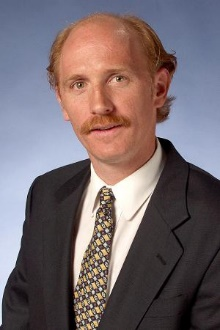
\includegraphics[width=1in,height=1.5in]{./Fig/image2.jpeg}Chris
Coulston obtained his Ph.D. in Computer Science and Engineering from the
Pennsylvania State University in 1999. He obtained his M.S. and B.S in
Computer Engineering from the Pennsylvania State University in 1994 and
1992 respectively. Chris has industry experience working for IBM in
Manassas, VA and Accu-Weather in State College, PA. He joined the
faculty at Penn State Erie, The Behrend College in 1999. He has
experience teaching design-oriented courses in digital systems, embedded
systems, computer architecture, and database management systems. Chris'
research interests are in Steiner tree routing algorithms and artificial
life. He is currently an Associate Professor of Electrical and Computer
at Penn State Behrend and also serves as Chairperson of the program.


\tableofcontents
%% \section{Preface}\label{preface}

This book is written for undergraduate students and teachers engaged in
electrical and computer engineering (ECE) design projects, primarily in
the senior year. The objective of the text is to provide a treatment of
the design process in ECE with a sound academic basis that is integrated
with practical application. This combination is necessary in design
projects because students are expected to apply their theoretical
knowledge to bring useful systems to reality. This topical integration
is reflected in the subtitle of the book: Theory, Concepts, and
Practice. Fundamental theories are developed whenever possible, such as
in the chapters on functional design decomposition, system behavior, and
design for reliability. Many aspects of the design process are based
upon time-tested concepts that represent the generalization of
successful practices and experience. These concepts are embodied in
processes presented in the book, for example, in the chapters on needs
identification and requirements development. Regardless of the topic,
the goal is to apply the material to practical problems and design
projects. Overall, we believe that this text is unique in providing a
comprehensive design treatment for ECE, something that is sorely missing
in the field. We hope that it will fill an important need as capstone
design projects continue to grow in importance in engineering education.

We have found that there are three important pieces to completing a
successful design project. The first is an understanding of the design
process, the second is an understanding of how to apply technical design
tools, and the third is successful application of professional skills.
Design teams that effectively synthesize all three tend to be far more
successful than those that don't. The book is organized into three parts
that support each of these areas.

The first part of the book, the \emph{Design Process}, embodies the
steps required to take an idea from concept to successful design. At
first, many students consider the design process to be obvious. Yet it
is clear that failure to understand and follow a structured design
process often leads to problems in development, if not outright failure.
The design process is a theme that is woven throughout the text;
however, its main emphasis is placed in the first four chapters. Chapter
1 is an introduction to design processes in different ECE application
domains. Chapter 2 provides guidance on how to select projects and
assess the needs of the customer or user. Depending upon how the design
experience is structured, both students and faculty may be faced with
the task of selecting the project concept. Further, one of the important
issues in the engineering design is to understand that systems are
developed for use by an end-user, and if not designed to properly meet
that need, they will likely fail. Chapter 3 explains how to develop the
Requirements Specification along with methods for developing and
documenting the requirements. Practical examples are provided to
illustrate these methods and techniques. Chapter 4 presents concept
generation and evaluation. A hallmark of design is that there are many
potential solutions to the problem. Designers need to creatively explore
the space of possible solutions and apply judgment to select the best
one from the competing alternatives.

The second part of the book, \emph{Design Tools}, presents important
technical tools that ECE designers often draw upon. Chapter 5 emphasizes
system engineering concepts including the well known functional
decomposition design technique and applications in a number of ECE
problem domains. Chapter 6 provides methods for describing system
behavior, such as flowcharts, state diagrams, data flow diagrams and a
brief overview of the Unified Modeling Language (UML). Chapter 7 covers
important issues in testing and provides different viewpoints on testing
throughout the development cycle. Chapter 8 addresses reliability theory
in design, and reliability at both the component and system level is
considered.

The third part of the book focuses on \emph{Professional Skills}.
Designing, building, and testing a system is a process that challenges
the best teams, and requires good communication and project management
skills. Chapter 9 provides guidance for effective teamwork. It provides
an overview of pertinent research on teaming and distills it into a set
of heuristics. Chapter 10 presents traditional elements of project
planning, such as the work breakdown structure, network diagrams, and
critical path estimation. It also addresses how to estimate manpower
needs for a design project. Chapter 11 addresses ethical considerations
in both system design and professional practice. Case studies for ECE
scenarios are examined and analyzed using the IEEE (Institute of
Electrical and Electronics Engineers) Code of Ethics as a basis. The
book concludes with Chapter 12, which contains guidance for students
preparing for oral presentations, often a part of capstone design
projects.

\textbf{Features of the Book}

This book aims to guide students and faculty through the steps necessary
for the successful execution of design projects. Some of the features
are listed below.

\begin{itemize}
\item
  Each chapter provides a brief motivation for the material in the
  chapter followed by specific learning objectives.
\item
  There are many examples throughout the book that demonstrate the
  application of the material.
\item
  Each end-of-chapter problem has a different intention. Review problems
  demonstrate comprehension of the material in the chapter. Application
  problems require the solution of problems based upon the material
  learned in the chapter. Design problems are directly applicable to
  design projects and are usually tied in with the Project Application
  section.
\item
  Nearly all chapters contain a Project Application section that
  describes how to apply the material to a design project.
\item
  Some chapters contain a Guidance section that represents the author's
  advice on application of the material to a design project.
\item
  Checklists are provided for helping students assess their work.
\item
  There are many terms used in design whose meaning needs to be
  understood. The text contains a glossary with definitions of design
  terminology. The terms defined in the glossary (Appendix A) are
  indicated by \emph{\textbf{italicized-bold}} highlighting in the text.
\item
  All chapters conclude with a Summary and Further Reading section. The
  aim of the Further Reading portion is to provide pointers for those
  who want to delve deeper into the material presented.
\item
  The book is structured to help programs demonstrate that they are
  meeting the ABET (accreditation board for engineering programs)
  accreditation criteria. It provides examples of how to address
  constraints and standards that must be considered in design projects.
  Furthermore, many of the professional skills topics, such as teamwork,
  ethics, and oral presentation ability, are directly related to the
  ABET Educational Outcomes. The requirements development methods
  presented in Chapter 3 are valuable tools for helping students perform
  on cross-functional teams where they must communicate with
  non-engineers.
\item
  An instructor's manual is available that 
  contains not only solutions, but guidance from the authors on teaching
  the material and managing student design teams. It is particularly
  important to provide advice to instructors since teaching design has
  unique challenges that are different than teaching engineering science
  oriented courses that most faculty are familiar with.
\item
  PowerPoint\textsuperscript{TM} presentations are available for
  instructors through McGraw-Hill
\item
  There are a number of complete case study student projects available
  in electronic form for download by both students and instructors and
  available at.
  These projects have been developed using the processes provided in
  this book.
\end{itemize}

\textbf{How to Use this Book}

There are several common models for teaching capstone design, and this
book has the flexibility to serve different needs. Particularly,
chapters from the Professional Skills section can be inserted as
appropriate throughout the course. Recommended usage of the book for
three different models of teaching a capstone design course is
presented.

\begin{itemize}
\item
  \textbf{Model I.} This is a two-semester course sequence. In the first
  semester, students learn about design principles and start their
  capstone projects. This is the model that we follow. In the first
  semester the material in the book is covered in its entirety. The
  order of coverage is typically Chapters 1--3, 9, 4--6, 10--11, and
  7--8. Chapter 9 (Teams and Teamwork) is covered immediately after the
  projects are identified and the teams are formed. Chapters 10 (Project
  Management) and 11 (Ethical and Legal Issues) are covered after the
  system design techniques in Chapters 5 and 6 are presented. Students
  are in a good position to create a project plan and address ethical
  issues in their designs after learning the more technical aspects of
  design. Chapter 12 (Oral Presentations) is assigned to students to
  read before their first oral presentation to the faculty. The course
  concludes with principles of testing and system reliability (Chapter 7
  and 8). We assign a good number of end-of-chapter problems and have
  quizzes throughout the semester. By the end of the first semester,
  design teams are expected to have completed development of the
  requirements, the high-level or architectural design, and developed a
  project plan. In the second semester, student teams implement and test
  their designs under the guidance of a faculty advisor.
\item
  \textbf{Model II}. This two-semester course sequence is similar to
  Model I with the difference being that the first semester is a lower
  credit course (often one credit) taught in a seminar format. In this
  model chapters can be selected to support the projects. Some of the
  core chapters for consideration are Chapters 1--5, which take the
  student from project selection to functional design, and Chapters
  9--11 on teamwork, project management, and ethical issues. Other
  chapters could be covered at the instructor's discretion. The use of
  end-of-chapter problems would be limited, but the project application
  sections and example problems in the text would be useful in guiding
  students through their projects.
\item
  \textbf{Model III}. This is a one-semester design sequence. Here, the
  book would be used to guide students through the design process.
  Chapters for consideration are 1--5 and 9--10, which provide the
  basics of design, teamwork, and project management. The project
  application sections and problems could be used as guidance for the
  project teams.
\end{itemize}

\textbf{Acknowledgements}

Undertaking this work has been a challenging experience and could not
have been done without the support of many others. First, we thank our
families for their support and patience. They have endured many hours
and late evenings that we spent researching and writing. Melanie Ford is
to be thanked for her diligent proofreading efforts. Bob Simoneau, the
former Director of the Penn State Behrend School of Engineering, has
been a great supporter of the book and has also lent his time in reading
and providing comments. Our school has a strong design culture, and this
book would not have happened without that emphasis; our faculty
colleagues need to be recognized for developing that culture. Jana
Goodrich and Rob Weissbach are two faculty members with whom we have
collaborated on other courses and projects. They have influenced our
thinking in this book, particularly in regard to project selection,
requirements development, cost estimation, and teamwork. We must also
recognize the great collaborative working environment that exists at
Penn State Behrend, which has allowed this work to flourish. Our
students have been patient in allowing us to experiment with different
material in the class and on the projects. Examples of their work are
included in the book and are greatly appreciated. John Wallberg
contributed the disk drive diagnostics case study in Chapter 11 that we
have found very useful for in-class discussions. John developed this
while he was a student at MIT. Thanks to Anne Maloney for her
copyediting of the manuscript. 

Finally, we would like to thank the external reviewers of the book for
their thorough reviews and valuable ideas. They are Frederick C. Berry
(Rose-Hulman Institute of Technology), Mike Bright (Grove City College),
Geoffrey Brooks (Florida State University Panama City Campus) Wils L.
Cooley (West Virginia University), D. J. Godfrey (US Coast Guard
Academy), and Michael Ruane (Boston University).

We hope that you find this book valuable, and that it motivates you to
create great designs. We welcome your comments and input. Please feel
free to email us.

Ralph M. Ford, \href{mailto:rmf7@psu.edu}{\nolinkurl{rmf7@psu.edu}}

Christopher S. Coulston,
 \href{mailto:coulston@mines.edu}{\nolinkurl{coulston@mines.edu}}


\mainmatter 					% Now Use Arabic numerals for page numbers

\addcontentsline{toc}{chapter}{Part I - The Engineering Design Process }
\chapter*{Part I - The Engineering Design Process }

%
\chapter{The Engineering Design Process}
\section{The Engineering Design Process}
\graphicspath{ {./chapter01/Fig} }

\begin{itquote}
\textbf{en-gi-neer (n)} 
\textit{1. One versed in the design, construction, and
use of machines. 2. One who employs the innovative and methodical
application of scientific knowledge and technology to produce a device,
system, or process, which is intended to satisfy human needs.} ---American College Dictionary
\end{itquote}

Take a moment to read and analyze the key elements of the two
definitions presented above. If you are an engineering student or
practicing engineer, do you think that this definition applies to you?
The first definition uses the terms \emph{design} and
\emph{construction}. People like to think of themselves as designers.
Why is that so? The answer may be in the combination of the term
\emph{construction,} and from the second definition, the idea of
\emph{innovation}. Applying innovation and creativity to produce
something new is a wonderfully rewarding process. The great thing about
being an engineer is that it allows you to be a creative designer. That
is generally not the way the profession is viewed. What is the
difference between engineering design and other types of design that are
associated with creativity such as interior design, fashion design, or
webpage design? The answer is supplied in the second definition which
states \emph{''\ldots methodical application of scientific knowledge and
technology\ldots{}}'' As an engineering student, you have studied a
great deal of math, science, and fundamental technology, but probably
have had limited exposure to creative and innovative design.

The definition also contains the somewhat contradictory terms
\emph{innovative} and \emph{methodical}. If there is an established and
methodical way of employing a scientific principle or process, it does
not seem to allow much room for creativity and innovation. The truth is
that the two concepts are in competition with each other, but a good
engineer realizes this and utilizes both effectively. The definition
also indicates that engineers design to satisfy human needs, an
important, yet often overlooked point. That means that when designing
systems, it is necessary to determine the user's needs and the ethical
application of the technology.

This book aims to help electrical and computer engineers become
effective designers, to better understand professional practices, and to
provide guidance for executing design projects. This chapter presents
the processes by which designs are realized, the characteristics of
successful engineers, and an overview of the book.

\section*{Learning Objectives}
\noindent\rule{\linewidth}{1pt}
By the end of this chapter, the reader should:
\begin{itemize}
\item Understand what is meant by engineering design.
\item  Understand the phases of the engineering design process.
\item  Be familiar with the attributes of successful engineers.
\item  Understand the objectives of this book.
\end{itemize}

\section{The Engineering Design Process}

ABET (formerly known as Accreditation Board of Engineering and
Technology) provides the following definition of engineering design
{[}ABE03{]}.
\index{ABET}

\begin{quote}
Engineering design is the process of devising a system, component, or
process to meet desired needs. It is a decision-making process (often
iterative), in which the basic sciences, mathematics, and engineering
sciences are applied to convert resources optimally to meet a stated
objective. Among the fundamental elements of the design process are the
establishment of objectives and criteria, synthesis, analysis,
construction, testing, and evaluation.
\end{quote}

The definition indicates that, in engineering design, different phases
of the process have to be re-visited and the deliverables for each phase
updated as necessary. Realistic problems are complex with many potential
solutions; the goal is not to find just any solution, but the best one
given the constraints and available resources. This requires the
application of sound judgment, decision-making skills, and patience in
constantly evaluating progress towards a solution. The definition
identifies some common elements of the design process, such as
establishment of criteria, synthesis, construction, and testing.

\emph{\textbf{Design processes}} embody the steps required to take an
idea from concept to realization of the final system, and are
problem-solving methodologies that aim to develop a system that best
meets the customer's need within given constraints. This is not all that
different from some everyday processes, such as preparing dinner. Say
you are hungry and need to eat dinner before you can go to see a movie
that starts in one hour. The constraints are time, money, food, your
tastes, and nutritional value if you are health-conscious. You
brainstorm and come up with the options of making dinner at home, going
to a restaurant, or buying something to eat at the theater. Based on
these options, you then select the solution based on your evaluation of
the best one. This is similar in philosophy to the stages of design
processes where you have a problem to solve, constraints, and a number
of potential solutions to select from.

A related term is known as the \emph{product realization process}. The
product realization process is broader in scope, including aspects such
as entrepreneurship, market research, financial planning, product
pricing, and market strategy. Many technologies have their own
particular design processes that have evolved over time and have been
found by practitioners in the field to be valuable. For example,
different methodologies are applied in the design of integrated circuits
(VLSI), embedded systems, and software systems, yet they all have some
degree of commonality, such as requirements analysis, technical design,
and system test. Design processes continue to evolve. One field in which
this is particularly true is in software design due to the constantly
changing nature of software and the special challenges that large
software projects pose.

Cross {[}Cro00{]} identified two types of design
processes---prescriptive and descriptive. As the name implies,
\emph{\textbf{prescriptive design processes}} set down an exact process,
or systematic recipe, for realizing a system. Prescriptive design
processes are often algorithmic in nature and expressed using flow
charts with decision logic. An example of a prescriptive process is
shown in Figure~\ref{figure:prescriptiveDesign}, 
which describes the front end of the design process
where the problem and requirements are determined. A decision block is
included where the requirements are examined to determine if they
satisfy the needs of the problem. \emph{\textbf{Descriptive processes}}
are less formal, describing typical activities involved in realizing
designs with less emphasis on exact sequencing. The distinction between
descriptive and prescriptive processes is not always clear, however, and
some processes may be considered more strongly associated with one
property than the other. Cross makes an important point in stating that
design processes are sometimes viewed as common sense and thus ignored,
resulting in failed products. Cross cites two good reasons to adhere to
design processes: 1) they formalize thought processes to ensure good
practices are followed, leading to better and more innovative solutions,
and 2) they keep all members of the team synchronized in terms of
understanding where they are in the design process.

\begin{figure}[h]
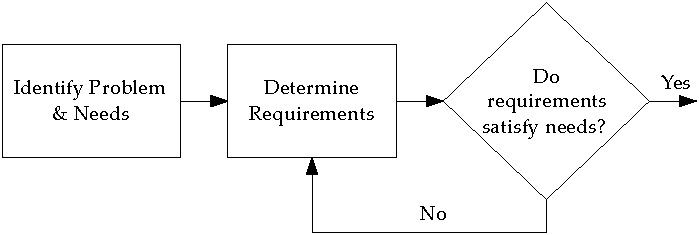
\includegraphics[width=3.8in,height=1.27in]{image1}
\caption{A prescriptive design process for problem
identification and requirements selection.}
\label{figure:prescriptiveDesign}
\end{figure}

A descriptive process that is widely applicable to design problems is
shown in Figure~\ref{figure:overviewDesignProcess}. 
In a perfect world, the process starts with the
identification of the problem, proceeds clockwise to research, followed
the requirements phase, and so on until the system or device is
delivered and goes into service (maintenance phase). This scenario is
unrealistic, ignoring the iterative nature of design where the design
team alternates between different phases as necessary. Consequently,
links are inserted that allow transitions between all the different
phases of the

\begin{figure}[h]
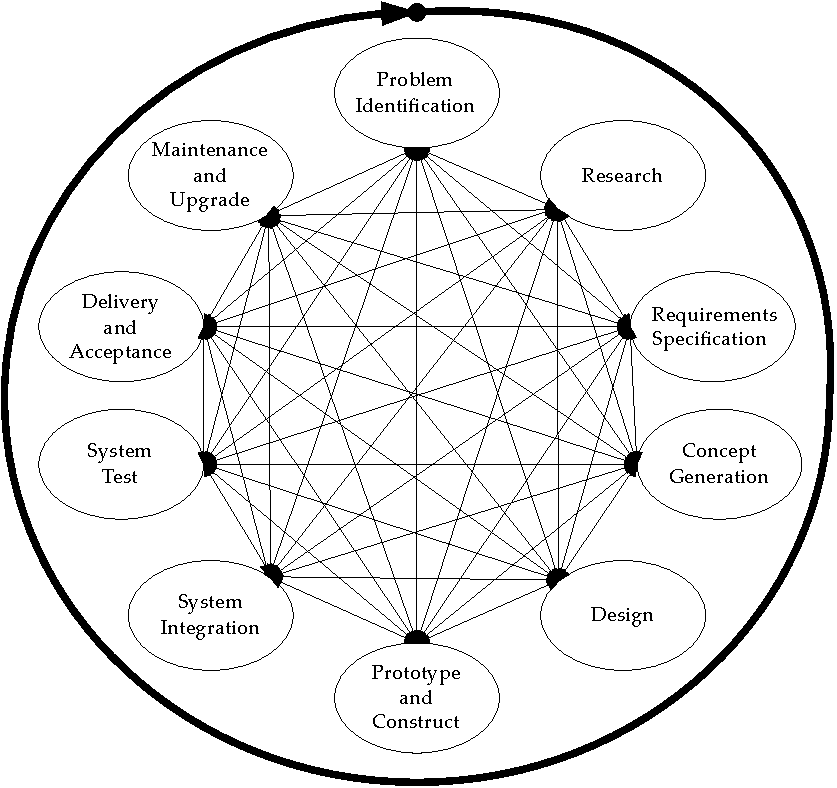
\includegraphics[width=5in,height=4.7in]{image2}
\caption{ A descriptive overview of the design process.}
\label{figure:overviewDesignProcess}
\end{figure}

design process. Of course, transitions between certain phases are
unreasonable or very costly. It is virtually impossible to move directly
from problem identification to system integration without developing a
design concept first. It is much more likely for engineers to alternate
between nearby phases in the process, such as problem identification,
research, requirements specification, and concept generation. This does
not mean that you can't move between phases that are not in close
proximity in the model. For instance, the customer's needs may change
while in the design phase, necessitating re-evaluation of the needs,
correction of the requirements specification, and system redesign---all
at a substantial cost in time and money. Studies have shown that the
cost required to correct errors or make changes increases exponentially
as the project lifetime increases, as presented in Figure~\ref{figure:costVsLife}.

\begin{figure}[h]
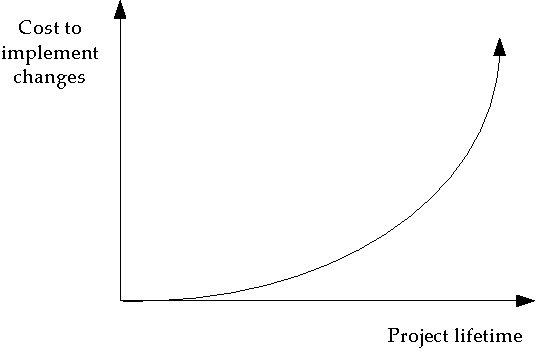
\includegraphics[width=3in,height=2in]{image3}
\caption{The cost to implement design changes increases exponentially with project lifetime.}
\label{figure:costVsLife}
\end{figure}

\subsection{Elements of the Design Process}

Nearly all the phases of the design process in Figure~\ref{figure:overviewDesignProcess} 
are covered in this book, with the exception of the maintenance phase. The objective of
the first phase, \emph{\textbf{problem identification}}, is to identify
the problem and customer needs. This occurs in a variety of ways, from
someone conceiving a new idea to a client coming to you with a problem
to solve. In either case, it is important to determine the true needs
for the product, device, or system (terms that are used interchangeably
throughout the book and often referred to as systems). Failure to
correctly identify the needs has negative ramifications for the entire
process, typically resulting in costly redesigns, or even worse,
abandonment of the project.

In the \emph{\textbf{research phase}} the design team conducts research
on the basic engineering and scientific principles, related
technologies, and existing solutions. The objective is to become experts
on the problem, save time and money by not re-inventing the wheel, and
be positioned to develop new and innovative solutions.

The \emph{\textbf{Requirements Specification}} articulates what the
system must do for it to be successful and to be accepted by the
customer. It is important to focus on what the system must do, as
opposed to how the solution will be implemented. This is challenging
since engineers tend to focus on solutions and propose implementations
early in the process. This is not surprising since engineering education
focuses on solving problems rather than specifying them. The
requirements are the mission statement that guides the entire project,
and if properly developed, provide flexibility for creativity and
innovation in developing solutions.

In \emph{\textbf{concept generation},} many possible solutions to the
problem are developed. The hallmark of design is that it is open-ended,
meaning that there are multiple solutions to the problem and the
objective is to develop the one that best meets the requirements and
satisfies the constraints. In this phase, wild creativity is encouraged,
but it is ultimately tempered with critical evaluation of the competing
alternatives.

In the \emph{\textbf{design phase},} the team iteratively develops a
technical solution, ultimately producing a detailed system design. Upon
its completion, all major systems and subsystems are identified and
described using an appropriate model that depends upon the particular
technology being employed.

In the \emph{\textbf{prototyping and construction phase},} different
elements of the system are constructed and tested. In rapid prototyping,
the objective is to model some aspect of the system, demonstrating
functionality to be employed in the final realization. Many prototypes
are discarded or modified as the system evolves---the idea is to
experiment, demonstrate proof-of-concept principles, and improve
understanding. Prototypes may be used anywhere in the process---you may
present the client with prototypes after the concept generation phase,
or they may be utilized in the design phase to test a design idea, or as
the final system is tested and developed.

During \emph{\textbf{system integration},} all of the subsystems are
brought together to produce a complete working system. This phase is
challenging and time-consuming since many different pieces of the design
must be interfaced, and the team must work closely to make it all work.
Care taken in the design phase to clearly communicate the functionality
and interfaces between subsystems aids in system integration. System
integration is closely tied to the \emph{\textbf{test phase}}, where the
overall system is tested to demonstrate that it meets the requirements.

Ultimately the system is \emph{delivered} to the customer where it is
likely that they will test it using a mutually agreed upon process.
Development does not necessarily end when the system goes into service,
as it will likely enter the \emph{\textbf{maintenance phase}} where it
is maintained, upgraded to add new functionality, or where design
problems are corrected. Following and understanding the design process
improves the probability of successful system development. The process
is flexible, and the designer needs to transition between different
phases in order to bring the system to realization. Design is an
iterative process---you may not fully understand everything necessary in
any given phase and have to revisit different steps as the system
evolves. That is not a license for not trying to develop the best design
you can on the first attempt---by all means do so---but realize that
flexibility and a willingness to change the design are necessary.

\subsection{Technology Specific Design Processes}

Different application domains have developed specialized processes for
technology-specific design. One such example is VLSI (Very Large Scale
Integration) design. A typical VLSI design process is shown in Figure~\ref{figure:VLSIdesign}
 {[}Wol02{]}. In this model the system specification is used to
develop the system architecture. The system architecture is composed of
the major functional units that constitute an integrated circuit. Each
functional unit is then designed at the gate logic level, which is
subsequently designed at the circuit (transistor) level, and finally the
circuit elements are laid out on the silicon chip. This is an excellent
demonstration of the divide-and-conquer approach to design, where a
complex system is broken down into lower levels of abstraction and each
of these is further broken down until the design objectives are met.

\begin{figure}[h]
 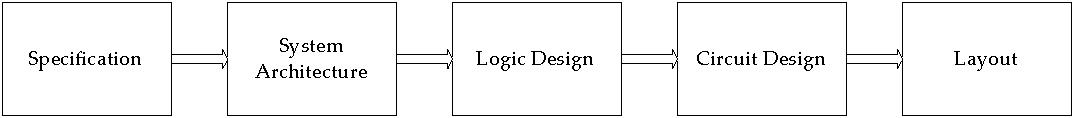
\includegraphics[width=5.5in,height=0.60417in]{image4}
\caption{A process for integrated circuit (VLSI) design {[}Wol02{]}.}
\label{figure:VLSIdesign}
\end{figure}

Next, consider the design process for embedded computer systems shown in
Figure~\ref{figure:embedded DesignProcess}. 
Embedded systems are combined hardware/software systems
embedded into a larger system to perform dedicated application specific
operations. Embedded systems are employed in automobiles, DVD players,
and digital cameras to name a few applications. Performance issues
dominate embedded applications, and the designer needs to partition
tasks between software and hardware to achieve optimum performance. This
design process is somewhat prescriptive with phases for requirements
gathering, specifications, and architectural design. The process
reflects the unique nature of embedded systems with separate software
and hardware design blocks, married together by the interface design.

\begin{figure}[h]
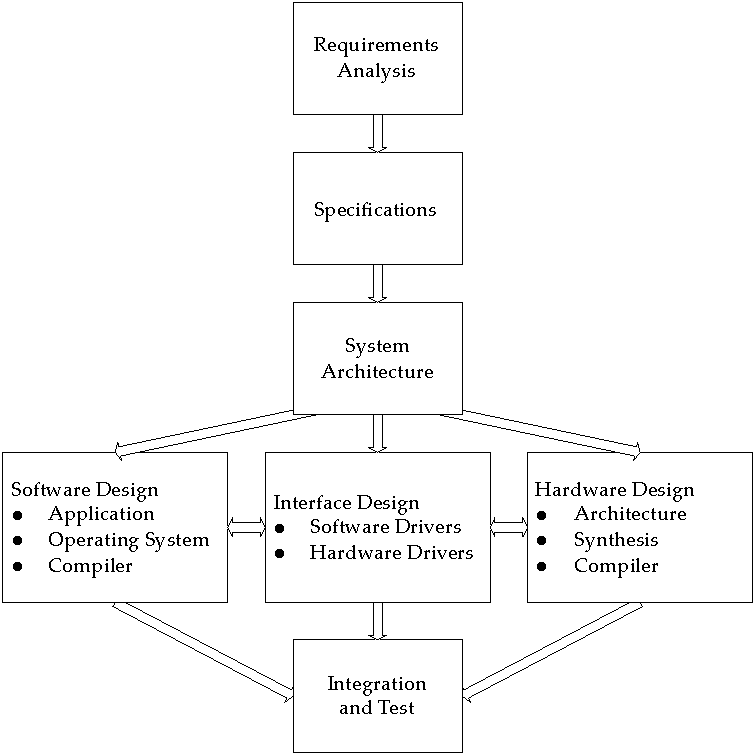
\includegraphics[width=3.8in,height=3.8in]{image5}
\caption{An embedded system design process {[}Ern97{]}.}
\label{figure:embedded DesignProcess}
\end{figure}

The field of software engineering is one in which the development of
different design process models is still under considerable flux today.
This is due to the complex nature of software and the failure of
computer scientists and engineers to effectively develop high-quality
software systems. There are many reasons why this is so. The sheer size
of software programs may easily exceed one million lines of code written
by many different software developers. One small mistake in those
millions of lines of code can cause the system to fail. Another
difficulty is in designing for upgrade and reuse of software. What if
the needs change after the millions of lines of code are developed and
one of the fundamental structures or objects needs to be upgraded?

The \emph{waterfall model} shown in Figure~\ref{figure:waterfallDesignProcess} 
is one of the first
proposed and most well-known software design processes. This is a
prescriptive model since the development proceeds linearly from the
first step where the user's needs are analyzed through the phases of
specification development, design, test, and maintenance. This works for
well-defined and moderately complex software applications, but fails as
complexity grows due to the inability to move between phases. A more
flexible and descriptive software design process is known as the
\emph{spiral model}, which is a cyclical process where phases are
revisited as necessary {[}Som01{]}. \emph{Extreme Programming} is a more
recent and controversial software development process, where relatively
small teams of software developers rapidly develop software following
some strict rules. Both the spiral model and Extreme Programming are
examined in more detail in the end of chapter problems.

\begin{figure}[h]
 
\includegraphics[width=4.6in,height=3.1in]{image6}
\caption{Waterfall software development process. In this
model, development proceeds linearly from requirements analysis, through
each subsequent phase, terminating with maintenance.}
\label{figure:waterfallDesignProcess}
\end{figure}

\section{The World-Class Engineer}\label{the-world-class-engineer}

The ability to effectively design is important for engineers, requiring
strong technical skills and an understanding of the design process. Yet,
this ability in itself is not enough to become an effective practicing
engineer. The Pennsylvania State University Leonhard Center for the
Advancement of Engineering Education, in consultation with a number of
industries, developed a description of what is referred to as a
``World-Class Engineer'' {[}Leo95{]}. Shown in Table~\ref{table:worldClassEngineer},
 the description identifies the characteristics of successful engineers, and
contains six major elements: 1) Aware of the World, 2) Solidly Grounded,
3) Technically Broad, 4) Effective in Group Operations, 5) Versatile,
and 6) Customer-Oriented. The description recognizes that engineers must
be effective in group operations, since the majority of projects are
carried out in teams. Not only that, many projects span multiple
technical disciplines and are executed in multifunctional organizations
that have diverse groups such as marketing, finance, human resources,
technical support, and service. It also recognizes that an engineer must
be versatile, innovative, understand ethical principles, and be
customer-oriented, important themes that are stressed throughout this
book.

\footnotesize
\begin{longtable}[c]{|m{14cm}|}
\caption{The World-Class Engineer (Copyright the Leonhard
Center for the Advancement of Engineering Education, The Pennsylvania
State University. Reprinted by permission.) 
\label{table:worldClassEngineer}}\\


\hline
\rowcolor{Gray}
\textbf{World Class Engineer} \\ \hline
\endfirsthead

\hline
\rowcolor{Gray}
{{\bfseries \tablename\ \thetable{} -- continued from previous page}} \\ \hline
\rowcolor{Gray}
\textbf{World Class Engineer} \\ \hline
\endhead
\endfoot

\hline

\begin{enumerate}
\itemsep0em 
\def\labelenumi{\Roman{enumi})}

\item Aware of the World 
\begin{itemize}
\itemsep0em 
\item  sensitive to cultural differences, environmental concerns, and ethical  principles
\item  alert to market opportunities (both high- and low-tech)
\item  cognizant of competitive talents, work ethic, and motivation
\end{itemize}

\item Solidly Grounded
\begin{itemize}
\itemsep0em 
\item  thoroughly trained in the fundamentals of a selected engineering
  discipline
\item  has a historical perspective and remains aware of advances in science
  that can impact engineering
\item  realizes that knowledge doubles at breakneck speed and is prepared to
  continue learning throughout a career
\end{itemize}

\item Technically Broad
\begin{itemize}
\itemsep0em 
\item  understands that real-life problems are multidisciplinary
\item  thinks broadly, seeing an issue in a rich context of various
  alternatives, probabilities, etc., rather than a narrow quest to find
  a single answer
\item  is conversant in several disciplines
\item  is trained in systems modeling and the identification of critical
  elements. Understands the need to design experiments to verify or
  extend analysis, as well as meet specification requirements
\item  is psychologically prepared to embrace any field necessary to solve
  the problem at hand
\end{itemize}

\item Effective in Group Operations
\begin{itemize}
\itemsep0em 
\item  cooperative in an organization of individuals working toward a common
  creative goal that is often multidisciplinary and multifunctional in
  nature
\item  effective in written and oral communication
\item   willing to seek and use expert advice
\item  cognizant of the value of time and the need to make efficient use of
  the time in all phases of an endeavor
\item   understanding and respectful of the many facets of business operation
  -\/- general management, marketing, finance, law, human resources,
  manufacturing, service, and especially quality
\end{itemize}

\item Versatile
\begin{itemize}
\itemsep0em 
\item  innovative in the development of products and services
\item  sees engineering as applicable to problem solving in general
\item  considers applying engineering beyond the typical employment focus of
  engineering graduates in the manufacturing industries, to the much
  broader economy (financial services, health care, transportation,
  etc.) where engineering skills could make a dramatic improvement in
  the productivity of those segments of the economy that employ 80
  percent of the U.S. population
\end{itemize}

\item Customer Oriented 
\begin{itemize}
\itemsep0em 
\item  realizes that finding and satisfying customers is the only guarantee
  of business success
\item  understands that products and services must excel in the test of
  cost-effectiveness in the global marketplace
\end{itemize}
\end{enumerate}
\\ \hline
\end{longtable}
\normalsize




\section{Book Overview}\label{book-overview}

Consider the digital camera, the cellular phone, and the space shuttle,
all complex systems that integrate a variety of technologies. A digital
camera is the synthesis of an embedded electronics system, optics, a
mechanical lens assembly, and the camera package itself. The embedded
electronics contain an imaging sensor, a digital display, digital
interface circuitry, flash memory storage, system control software, and
the user interface. The challenges of integrating the components of such
a system and having it record and transfer huge amounts of image data,
within an acceptable timeframe, are immense. Cellular phones are another
good example of a complex system that represents a technology that has
shrunk in size, but increased tremendously in functionality at the same
time. They encompass digital data communications, antenna design,
encryption for secure data transmission, a user interface display, and
Internet connectivity. At the other end of the spectrum are large-scale
space and military systems, such as the space shuttle. Despite the two
shuttle accidents, the safety and reliability requirements of the space
shuttle are incredibly high. Realizing such a system is accomplished by
a tremendous number of people from many disciplines working for
different organizations. All three of these technologies were developed
by large teams that encompass multiple disciplines. The processes and
practices employed in their development represent application of the
fundamentals that this book hopes to cover. While you won't be building
complete space shuttles by the end of this design course, you can expect
to apply design principles that allow you to design and integrate a
relatively complex system, maybe even a part of the space shuttle.


The intention is to teach the application of design principles to
computer and electrical engineers and to help prepare students for a
professional career. The majority of engineering education is devoted to
math, science, engineering science, and problem-solving. They are
important topics required to enter this highly technical field. However,
it is clear that there are other aspects beyond this that are equally
important for success, including an understanding of system design,
innovation, ethical principles, teamwork, and strong communication
skills.

The book is divided into three parts: I--Design Process, II--Design
Tools, and III--Professional Skills. This is shown in Figure~\ref{table:bookPhilosophy}
 as three separate, but related components that play a key role in achieving
Project Excellence---the ability to complete a project, in an ethical
manner that meets the customer's need, satisfies the constraints, and is
clearly communicated to all involved. The chapters are decoupled as much
as possible so that the reader can move between chapters as necessary.
In Part I, the emphasis is on understanding and gaining experience in
the different phases of the design process. The reader is guided through
the steps of project identification, research, specification
development, creative concept generation, and critical evaluation of
competing solutions. Part II addresses topics that are often employed in
design, including functional decomposition, description of system
behavior, reliability, and testing. Part III addresses professional
skills, including teamwork principles, project planning, ethics in
design and the profession, and oral communication skills.

\begin{figure}[h]
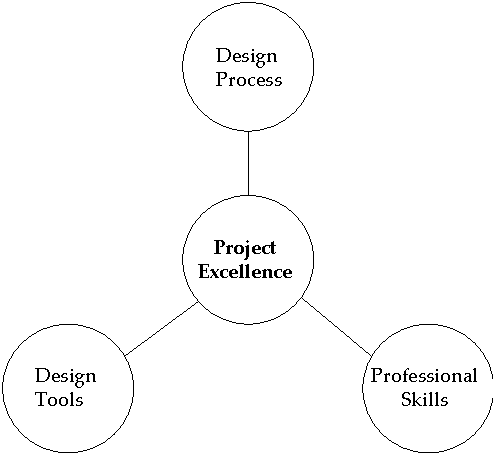
\includegraphics[width=2.875in,height=2.625in]{image7}
\caption{The guiding philosophy of this book. In order to
achieve success in executing engineering and design projects, it takes
an understanding of the design process, strong technical design tools,
and professional skills.}
\label{table:bookPhilosophy}
\end{figure}


Here are a few thoughts to conclude the chapter and get started on the
path to great designs. You are embarking on what will likely be a fun,
challenging, sometimes frustrating, and ultimately rewarding journey.
The systems that engineers work with continue to become increasingly
complex and multi-disciplinary in nature. The example problems presented
in this book come from the fields of analog electronics, digital
electronics, electrical systems theory, and software systems. These four
areas comprise a significant problem-domain common to the education of
most electrical and computer engineers. Finally, consider the quote
below by Robert Hayes on the importance of design.

Fifteen years ago, companies competed on price. Today it's quality.
Tomorrow it's design.---Robert H. Hayes, Harvard Business School, 1991.

What is this saying? Well, it is clear that the world continues to move
to a more knowledge-based society, where individuals and companies
compete on the strength of their intellectual capital and ability to
produce new and innovative products. That is what design is all about.
It is not saying that price and quality are unimportant, they certainly
are; in fact quality and reliability in design are part of this book. It
is that quality and price are a given, and successful products will be
distinguished by their design characteristics. The implication is that
design will play a larger role in the development and success of
products. The future Hayes predicted is now. Design is what
distinguishes between products that are seen as commodities and those
that are truly unique and profitable.

\section{Summary and Further
Reading}\label{summary-and-further-reading}

Engineering design is an iterative process in which the design team
employs creativity and technical knowledge to develop a solution that
best meets the end-users' needs within the constraints applied to the
problem. There is no single design process that can be applied to all
situations and technologies, but there are many common elements shared,
regardless of the technology under consideration. In order to
successfully bring designs to fruition, it takes a combination of design
tools, professional skills, and a clear understanding of the process
needed to complete designs. The objective of this book is to develop
your proficiency in these areas so that you may become an effective
engineer and achieve excellence in design projects.

\underline{Engineering Design Methods} by Nigel Cross {[}Cro00{]} presents the
differences between descriptive and prescriptive design processes, and
covers a wide array of processes in more detail. It also discusses the
cognitive characteristics of effective designers. There are many good
books on software engineering process development methods. \underline{Software
Engineering} by Ian Sommerville {[}Som01{]} discusses the different
software design process models, such as the waterfall and spiral models.
This is also true of many modern software engineering texts. The
original reference to the waterfall model is by Royce {[}Roy70{]}.
\underline{The Art of Innovation} by Michael Kelley {[}Kel01{]} describes the
activities of well-known design company IDEO and is a highly readable
description of their design practices. The ABC \emph{Nightline} news
program also produced an interesting segment on IDEO {[}ABC01{]} that
can be purchased at the ABC website. \underline{The Circle of Innovation} by
Tom Peters {[}Pet97{]} is another popular book that provides his
perspective on current trends in business and the importance of design.

%\section{Problems}
\label{problems}

\begin{enumerate}
\itemsep0em 
\def\labelenumi{\arabic{enumi}.}
\item
  In your own words, describe the difference between prescriptive and
  descriptive design processes. Cite examples of each.
\item
  Describe the relationship between the Problem Identification,
  Research, and Requirements Specification phases of the design process.
\item
  Describe the relationship between the Concept Generation and Design
  phases of the design process.
\item
  Construct a prescriptive design process for the Problem
  Identification, Research, Specification, Concept, and Design phases of
  the design process. The result should be a flow chart that contains
  decision blocks and iteration as necessary.
\item
  Describe the main differences between the VLSI and embedded system
  design processes.
\item
  Using the library or Internet, conduct research on the spiral software
  design process.

\begin{enumerate}
\itemsep0em 
\def\labelenumi{\alph{enumi})}
\item
  Outline the significant elements of the spiral software design
  process.
\item
  Describe the advantages and disadvantages of this relative to the
  waterfall model?
\end{enumerate}

\begin{quote}
Cite all reference used.
\end{quote}

\item
  Using the library or Internet, conduct research on the Extreme
  Programming design process.

\begin{enumerate}
\itemsep0em 
\def\labelenumi{\alph{enumi})}
\item
  Outline the significant elements of the Extreme Programming paradigm.
\item
  What are the pro and con arguments for this software development
  model?
\end{enumerate}

\begin{quote}
Be sure to cite references.
\end{quote}

\item
  \textbf{Project Application.} In preparation for project and team
  selection, develop a personal inventory that includes a list of five
  favorite technologies or engineering subjects that you are interested
  in pursuing. Also, list the strengths and weaknesses that you bring to
  a project team.
\end{enumerate}


%\chapter{Project Selection and Needs Identification}
\graphicspath{ {./chapter02/Fig} }

\begin{itquote}
For every problem there is a solution that is simple, neat, and
wrong.---H.L. Mencken
\end{itquote}

Traditionally, companies have organized resources based on functions
such as accounting, engineering, finance, manufacturing, and marketing.
It is often more effective to organize around projects that are of
significant value and align resources to meet the needs of the project.
This means that traditional departments and middle management are being
de-emphasized and the role of projects is growing. Capstone design
projects provide a great opportunity to gain experience in the
management and execution of a project. One of the first and most
important decisions encountered is selecting a project to pursue.

The objective of this chapter is to provide pragmatic guidance in the
project selection phase. A description of design and engineering
projects is presented, followed by advice on how projects can be
selected by engineering students who wish to put design principles into
practice. The chapter addresses how to identify the needs of the
end-user and provides guidance for conducting background research. All
of this information is brought together in a Problem Statement that
identifies the needs, the goals of the project, and research on the
technology.

\section*{Learning Objectives}
\noindent\rule{\linewidth}{1pt}
By the end of this chapter, the reader should:
\begin{itemize}
\item
  Have an understanding of the types of projects that electrical and
  computer engineers undertake.
\item
  Understand and be able to apply criteria for project selection.
\item
  Know how to determine, document, and rank end-user needs.
\item
  Be aware of resources available for conducting research surveys.
\item
  Have selected a project concept and developed a Problem Statement.
\end{itemize}

\section{Engineering Design Projects}
\label{section:engineering-design-projects}

This section provides a classification of design and describes some of
the types of projects undertaken by practicing engineers and those
tackled in student projects. In reality, most projects don't fit neatly
into the categories presented, but are some combination of them. The
objective of a design project is to create a new
\emph{\textbf{artifact}} (system, component, or process) to meet a given
need. Within the design domain there are different types of designs that
are classified broadly into three categories of Creative, Routine, and
Variant designs {[}Cro00{]}.

\emph{\textbf{Creative designs}} represent new and innovative products.
An example of a creative design is the Palm Pilot Personal Digital
Assistant (PDA). While the idea for the PDA had been around for awhile,
earlier attempts at developing the technology, notably the Apple Newton,
were unsuccessful. This was primarily due to unreliable handwriting
recognition that frustrated the user. However, Palm Computing had the
creative idea to develop a simplified handwriting language, Graffiti,
which eliminated the need for natural handwriting recognition. The Palm
Pilot is a great example of a creative design---it is simple (four basic
functions), fits in your pocket, and is easy to use. This innovation
spawned a huge hand-held computing industry.

\emph{\textbf{Variant designs}} are variations of existing designs,
where the intent is to improve performance or add features to an
existing system. Many engineering projects fall into this category. For
example, the objective may be to increase accuracy or system throughput.

\emph{\textbf{Routine designs}} represent the design of devices for
which theory and practice are well-developed. Examples are DC power
supplies, analog and digital filters, and basic digital components such
as adders and comparators. Routine designs are often components of more
complex creative and variant designs.

Within these three categories of design, there are many different types
of projects. \emph{Systems engineering and systems integration projects}
represent the synthesis of many subsystems into a larger system. They
may be creative or variant designs, but have unique challenges since
they are typically large and involve many people and technologies.
Adherence to good design processes is important for their success.
Engineers are often engaged in \emph{systems test}, where the objective
is to ensure that a system meets stated requirements and the needs of
the user. Examples include the testing of systems for use in space and
military environments.

The objective in \emph{experimental design} \emph{projects} is to design
experimental procedures and apparatus for determining the
characteristics of a system. For example, an engineering team may test a
system under a variety of operating conditions. Example 2.3 presented
later in the chapter is such a project, where the objective was to
design a series of experiments to test the feasibility of gigabit
Ethernet technology in a military environment. The test explored the
impact of environmental factors such as temperature and vibration, and
further used this data to estimate the operating lifetime of the
Ethernet board. Upon completion of this project, the team made
recommendations as to the allowable operating ranges of the technology.

The objective in \emph{analysis projects} is to analyze some aspect of
an existing system to improve or correct it. For example, a system or
process may be failing in the field and the source of the failure
unknown. Tools such as the Failure Mode Effects and Analysis technique
may be applied in this situation to identify the sources of failure. In
t\emph{echnology evaluation} \emph{projects}, technologies are assessed
to determine if they can be used in a given application. This may be to
determine if the technology can improve an existing system, or to
characterize its operating performance.

The objective of a \emph{research project} is to perform research or
experiments with the goal of discovering or creating a new technology.
The fundamental difference between this and other types of projects is
that the ultimate outcomes are unknown. Most engineering research falls
under the category of \emph{applied research}. This refers to the
creation of new technology or systems based on existing technology and
theory developed from fundamental research. \emph{Fundamental research}
emphasizes the discovery of new scientific principles without
necessarily having an intended application. Fundamental research is very
valuable, but not typically a part of design projects.

\section{Sources of Project Ideas}
\label{section:sources-of-project-ideas}

Depending upon your situation, you may have the opportunity to identify
and select your project. The list below provides some places to search
for project ideas:

\begin{itemize}
\item
  \emph{Industry sponsored projects.} Many companies will sponsor
  projects and are happy to do so, particularly if you have worked for
  them on an internship.
\item
  \emph{Engineers without Borders
  (\href{http://www.ewb-usa.org}{www.ewb-usa.org})}. This organization
  sponsors student projects to improve the quality of life in developing
  countries.
\item
  \href{http://www.FreeRandD.com}{\emph{www.FreeRandD.com}}. This is a
  clearinghouse for businesses and students teams to collaborate on
  projects. It allows businesses to post capstone project ideas for
  students to work on, while students can post resumes and project
  interests.
\item
  \emph{Your campus and local community.} In our school, a number of
  student teams have identified novel projects by asking other
  departments on campus for ideas. They have also been successful in
  approaching local community organizations for ideas, such as museums
  and research institutes.
\item
  \emph{Brainstorm.} Get together with a group of your peers and
  brainstorm on project ideas. You will be surprised at how many project
  ideas you can develop in a good brainstorming session (see Chapter 4).
  Do not only consider project ideas, but also brainstorm to identify
  problems that need solutions.
\end{itemize}

\section{Project Feasibility and Selection Criteria}
\label{section:project-feasibility-and-selection-criteria}

This section provides questions to consider when examining the
feasibility of a project. George H. Heilmeier (an electrical engineer
who has held positions as Chief Technology Officer of Texas Instruments,
Director of the Defense Advanced Research Projects Agency, and CEO of
Bellcore) developed a set of questions to answer when starting a new
project {[}Sha94{]}. Heilmeier argued that all projects must be tied to
the goals of the organization, and applied this by asking the following
questions:

\begin{itemize}
\item
  What are you trying to do? Articulate your goals using absolutely no
  jargon.
\item
  How is it done today, and what are the limitations of current
  practice?
\item
  What is new in your approach, and why do you think it will be
  successful?
\item
  Who cares? If you are successful, what difference will it make?
\item
  What are the risks and payoffs?
\item
  How much will it cost? How long will it take?
\item
  What are the midterm and final exams to check for success?
\end{itemize}

Heilmeier credits successful completion of projects that he managed to
answering these questions up-front and adhering to disciplined project
management processes.

A second perspective is offered from an organizational project
management viewpoint {[}Gra02{]} that provides the following criteria
for project selection:

\begin{itemize}
\item
  \emph{The project must be tied to the mission and vision of the
  organization.} Believe it or not, organizations often spend resources
  fruitlessly on projects that don't meet this criterion. To be fair,
  there is always risk associated with a project and it is sometimes
  hard to judge exactly how well a project meets this criterion. For
  engineers who are new to an organization, it is hard to judge a
  project's importance relative to the mission and goals, but if you
  find yourself in this situation, do not be afraid to ask some
  questions. Novices ask basic questions that are often overlooked by
  those who are highly experienced or intimately involved in a project.
\item
  \emph{Must have payback.} An economic analysis should be done to
  estimate if the project will make a profit. Much of this is outside
  the scope of this text, requiring marketing and financial analyses.
  Chapter 10 covers the basics of project cost estimation that will help
  in trying to answer this question.
\item
  \emph{Should have selection criteria.} Sound criteria for selecting
  among competing projects should be employed. The example at the end of
  this section demonstrates the application of criteria in project
  selection.
\end{itemize}

\begin{itemize}
\item
  \emph{Objectives of the Project should be SMART: Specific, Measurable,
  Assignable, Realistic, Time-Related}. Chapter 3 addresses how to
  determine project requirements that are Specific and Measurable.
  Assignable, Realistic, and Time-Related all refer to project
  management aspects that are covered in Chapter 10. The objective is to
  develop tasks that are assigned to groups or individuals and
  realistically can be completed in the given timeframe.
\end{itemize}

The following example demonstrates how to apply a project selection
model using a method known as the Analytical Hierarchy Process. AHP is a
decision making method that is described in Appendix B and is utilized
frequently throughout the text -- \textbf{the reader should read
Appendix B prior to proceeding with this example}.

\cbstart

\textbf{Example 2.1} A project selection model for capstone design.

Assume that you are part of a capstone design team that has the
opportunity to select their project from competing project ideas. The
steps in making a decision using AHP are to select the criteria that
drive the decision, determine relative weights of the criteria, rate the
alternatives (in this case project concepts) against the criteria, to
compute a weighted score for each of the alternatives, and then review
the decision.

\ul{Step 1: Determine the selection criteria}

To select the criteria, assume that the team brainstorms to determine
the following criteria that interest the team members:

\begin{quote}
A -- Match to team skills

B -- Technical complexity

C -- Creativity

D -- Market potential

E -- Industry sponsorship
\end{quote}

\ul{Step 2: Determine the criteria weightings}

Assume the team applies the method of pairwise comparison to determine
the weights as shown in Appendix B. In order to do so, the team
systematically compares each criterion to all others using the following
scale of relative importance:

1 = equal, 3 = moderate, 5 = strong, 7 = very strong, 9 = extreme.

Again, details of pairwise comparison are outlined in Appendix B and the
results are below. \\


\begin{tabular}{ |> {\columncolor{Gray}} c  |c|c|c|c|c|c|} 
\hline
\rowcolor{Gray}
Criteria & A & B & C & D & E & Weight \\ 
\hline
A & 1 & 5 & 5 & 3 & 3 & 0.52 \\
\hline
B & 1/5 & 1 & 3 & 1/3 & 1/3 & 0.12 \\
\hline
C & 1/5 & 1/3 & 1 & 1 & 3 & 0.09 \\
\hline
D & 1/3 & 3 & 1 & 1 & 5 & 0.18 \\
\hline
E & 1/3 & 3 & 1/3 & 1/5 & 1 & 0.09 \\
\hline
\end{tabular}
\\

This is an important step and one often overlooked -- the team has
identified what is important to it in project selection. It is clear
that match to the team skills (criterion A) is most important, by a
large margin, followed by market potential.

\ul{Step 3: Identify and rate alternatives relative to the criteria}

Assume that the team identifies three potential projects ideas: 1 --
IEEE sponsored robot competition, 2 -- Industry sponsored project to
design a new test protocol, and 3 -- Design of an item-finder device to
help people locate lost items. Furthermore, the team goes through the
process of rating each project relative to the criteria as outlined in
Appendix B. These ratings are reflected in the decision matrix in the
next step.

\ul{Step 4: Compute scores for the alternatives}

The decision matrix below is constructed and the scores for the
alternatives determined.


\begin{tabular}{|l|c|c|c|c|}
\hline
\rowcolor{Gray}
\multirow{ 2}{*}{Selection Criteria} & \multirow{ 2}{*}{Weights} & \multicolumn{3} {|c|} {Alternatives} \\ \hline

\rowcolor{Gray}
                                                           &                                              & Project 1 & Project 2 & Project 3 \\ \hline
A (Match to skills) & 0.52 & 0.40 & 0.20 & 0.40 \\  \hline
B (Technical Complexity) & 0.12 & 0.40 & 0.30 & 0.30 \\ \hline
C (Creativity) & 0.09 & 0.45 & 0.20 & 0.35 \\ \hline
D (Market potential) & 0.18 & 0.05 & 0.35 & 0.60 \\ \hline
E (Industry sponsorship) & 0.09 & 0.00 & 1.0 & 0.00 \\ \hline
Score & & 0.31 & 0.31 & 0.38 \\ \hline
\end{tabular}


\ul{Step 5: Review the decision}

Project 3 (item finder) is rated the highest among the three choices
based upon the weights determined by the team members. It is a good
match to the team skills, but also matches their desire to solve a
problem with good market potential. The remaining two projects are rated
about equal.
\cbend

\section{Needs Identification}
\label{section:needs-identification}

Often a customer, client, or supervisor comes to you with a problem to
solve and you must determine the needs or requirements for the solution
to the problem. In other words, determine the \emph{voice of the
customer}. This seems like a simple statement---ask the customer what
they want and you are done, right?

As an illustration, let's say a client comes to you with the following
request---\emph{The traffic at the front of campus is too congested. I
would like you to design a new traffic lane for northbound traffic
exiting at the intersection at the front of the college.} So you design
this new lane and have it added to the intersection. However, you find
out three months later that the traffic congestion has decreased a
little bit, but it is still a significant problem. So what went wrong?
Clearly you did what was asked of you, but the problem was not solved,
meaning that you were solving the wrong problem. The real problem was to
improve the flow of traffic at the entrance. In this case, the client
gave both the problem and the solution all in one statement. That is
fine if a careful feasibility study was done and it was known that the
additional traffic lane would alleviate the problem, but that was not
the case here. This hypothetical situation is not so far fetched and
happens in practice via neglect to do the up-front research or because
underlying assumptions change. The point is that the \ul{correct}
problem should be identified and solved.

It would be better if the client had simply asked to improve the traffic
flow, providing the opportunity to analyze the situation and develop
different design options. Some questions to be asked in this situation
are: \emph{How much additional traffic is there? At what times does this
happen? Where is the traffic coming from? What is an acceptable waiting
time at the intersection?} It may be that several new lanes are needed,
or perhaps the sequencing of the traffic signals is wrong, or maybe a
new entrance could be added for less cost and improved traffic flow.

The lesson is that customers often come with the problems and solution
all wrapped up together. When this is done, the \emph{\textbf{design
space}}, the space of all possible solutions to the problem, is
unnecessarily limited. Be ready to tactfully challenge the assumptions
and ask questions to get to the root of the problem. Ask clarifying
questions, analyze, pick apart the request, and focus on the problem,
not the solution.

Researchers and practitioners have examined the problem of eliciting
needs, and it is an important pre-requisite for developing good
engineering requirements specifications. Ulrich and Eppinger {[}Ulr03{]}
proposed a process for obtaining the \emph{voice of the customer} using
the following five steps: 1) Gather raw data from users; 2) Interpret
raw data in terms of needs; 3) Organize needs into a hierarchy; 4)
Determine the relative importance of the needs; and 5) Review the
outcomes and the process. Each of these steps is described in the
following sections.

\subsection*{ Step 1: Gather Raw Data from Users}

\textbf{DILBERT\textsuperscript{®} by Scott Adams}

\begin{figure}[h]

\includegraphics[width=5.5in,height=1.9in]{image1.png}
\caption{ The difficulties of communicating with the customer. (Dilbert © United Feature Syndicate. Reprinted by
permission.)}
\label{figure:dilbertCommunication}
\end{figure}


This is often accomplished via interviews with supervisors, key users,
or people from the client organization. In cases where new products are
being developed, focus groups are often employed. The advantage of
interviews and focus groups is that they provide the opportunity for
dialogue with the user where new ideas, concepts, and needs may emerge.
Another option is direct observation, where the team goes out and
examines the system in use and develops concepts for improving it. IDEO
Corporation is an innovative and successful company that designs new
products and systems. They rely heavily on direct observation as a
technique for successfully developing innovative products {[}Kel01{]}.
For example, IDEO was asked by a client to develop a new medical
instrument for balloon angioplasty used in hospital operating rooms. A
critical requirement from the user was that only one hand could be used
to operate the device because the technician's other hand had to be free
during the procedure. From direct observation, the IDEO design team
found that even though the current system was designed for one-hand use,
it was impractical, and the technicians actually used both hands. IDEO
designed and developed a two-handed pump that not only worked better
than the one handed pump, but was quieter, easier to read, and had
increased precision. This is another example of the customer specifying
the solution as part of the problem statement.

Ulrich and Eppinger provide the following questions to ask during an
interview:

\begin{itemize}
\item
  When and why do you use this type of product (system)?
\item
  Walk us through a typical session using the product.
\item
  What do you like about the existing products?
\item
  What do you dislike about the existing products?
\item
  What issues do you consider when purchasing the product?
\item
  What improvements would you make to the product?
\end{itemize}

\subsection*{Step 2: Interpret the Raw Data in Terms of Needs}


In this step the raw data is translated into customer needs. The needs
are expressed in terms of what the system must do (a requirement) as
opposed to how it is done. Statements of the customer's needs are known
as \textbf{\emph{marketing requirements}} or \emph{\textbf{marketing
specifications}}. For example, ``\emph{The system should have
high-quality audio}'' is a need or marketing requirement from the
customer regarding performance, but says nothing about how it will be
achieved. Marketing requirements are short sentences that describe the
need in the language of the customer. They typically do not have a
numerical target and are described as a state of being for the system.
Other examples of marketing requirements are, ``\emph{The system should
be easy-to-use,}'' and ``\emph{The system should be able survive a drop
from the runner's height.}''

\subsection*{Step 3: Organize Needs into a Hierarchy}

The marketing requirements are organized into a hierarchy of needs
arranged from the most general to the most specific in successive levels
of detail as required by the problem. It is organized by functional
similarity, not as hierarchy of importance (that is the next step). This
hierarchy is referred to as an \emph{\textbf{objective tree}}. An
example objective tree for a portable audio device intended for use by
runners is shown in Figure~\ref{figure:audioPortable}. The three high-level objectives
determined were high-quality audio, portable, and easy-to-use. Each of
these is further sub-divided into the characteristics that support the
higher level. For example, portability is divided into the needs of
lightweight, small, ergonomic, and the ability to operate in the
environment. The environmental need is further expanded into needs that
support it.

\begin{figure}[h]
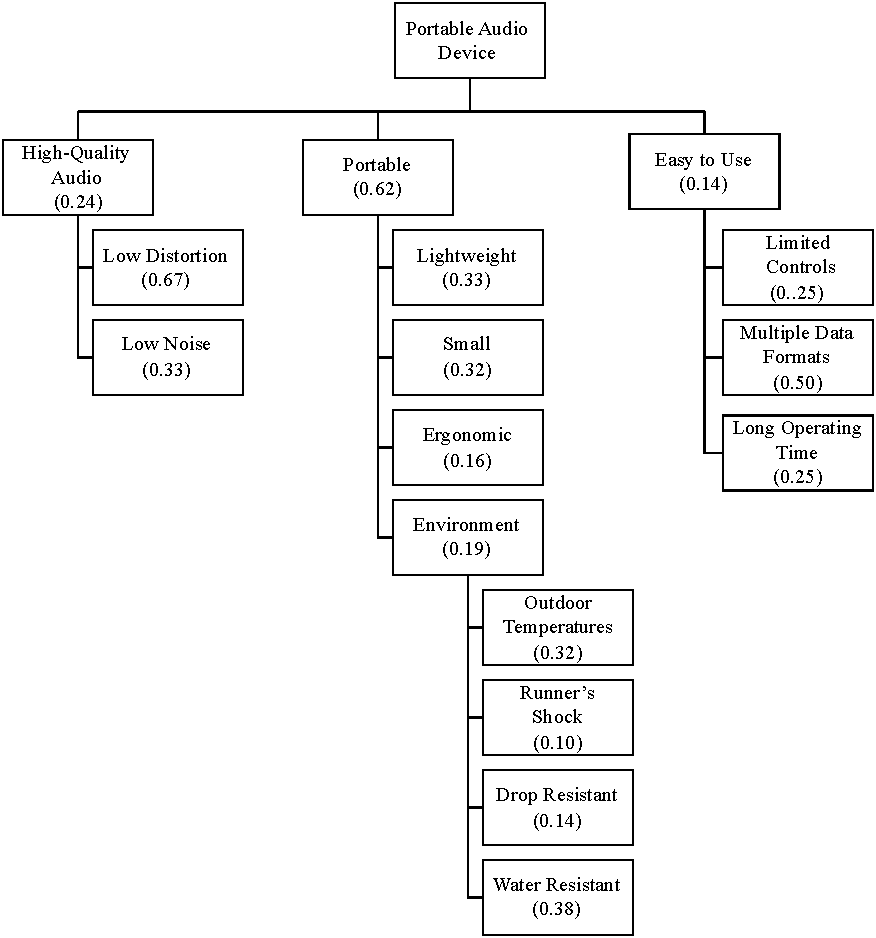
\includegraphics[width=5.2in,height=5.6in]{image2}
\caption{Objective tree for a portable audio device to be
used by runners. The weights reflect the relative importance of needs at
each level in the hierarchy as determined in Step 4 of the
process.}
\label{figure:audioPortable}
\end{figure}

\subsection*{Step 4: Determine the Relative Importance of the Needs}


The relative importance of the needs is determined based upon the user
needs. As we saw in Example 2.1 and as presented in Appendix B, the
pairwise comparison is a good technique for determining relative
importance and weighting of needs. In pairwise comparison, all needs are
systematically compared to all other needs at the same level in the
hierarchy. An example pairwise comparison table for this problem is
shown in Table~\ref{table:highQualityAudio} 
with the resulting weights for each need indicated.
This shows that portability is the most important need, followed by
audio quality and ease-of-use. The weights are also reflected in the
objective tree in Figure~\ref{figure:audioPortable}. In addition, the needs at each sublevel in
the hierarchy are compared, the results of which are reflected in 
Figure~\ref{figure:audioPortable}. The rankings are used in later chapters to compare design
alternatives.

\begin{table}[h]
\centering
\begin{tabular} {|> {\columncolor{Gray}} l|c|c|c||c|}
\hline
\rowcolor{Gray}
                             & High-Quality Audio & Portable & Easy-to-Use & Weight \\
\hline
High-Quality Audio & 1 & 1/3 & 2 & 0.24 \\
\hline
Portable & 3 & 1 & 4 & 0.62 \\
\hline
Easy-to-Use & 1/2 & 1/4 & 1 & 0.14 \\
\hline
\end{tabular}
\caption{Pairwise comparison matrix for ranking the
highest-level needs of the portable audio device. This comparison should
be carried out for all levels of the objective tree.}
\label{table:highQualityAudio}
\end{table}


\subsection*{Step 5: Review the Outcomes and the Process}

The design process and all of its sub-processes are methods for making
good decisions, and this technique for needs identification is no
different. There is a certain amount of subjectivity and judgment that
goes into it; the end result should be reviewed to determine if it makes
sense. The objective is to challenge assumptions, fully identify the
problem, and make informed decisions.

The three outcomes of this process are the marketing requirements that
identify the needs, an objective tree that provides a hierarchical
representation of the needs, and a ranking of the relative importance of
needs. This process may seem as though it does not apply to student
design projects, but in reality it does. The questions in this chapter
are certainly candidates to ask when working on company-sponsored
projects. If it is not a company sponsored project, the user needs
should still be considered. For example, questions can be asked of
friends and co-workers who are potential users of the system, focus
groups can be formed, surveys administered, and Internet bulletin boards
and discussion groups employed to gather this information.

\section{The Research Survey}
\label{section:the-research-survey}

It is important to conduct a thorough research survey while defining the
project concept. Failure to do so may translate into time and money
spent reinventing the wheel, while not taking full advantage of existing
components, knowledge, practices, and technology. During the research
phase, competing systems and technologies are identified, and based upon
them the project concept refined, or in some cases abandoned. The
character and strategy of the research survey is driven by the nature of
the project. In general, the objective is to develop an understanding of
the underlying scientific principles and demonstrate a familiarity with
the state-of-the-art in the particular field. Some questions to be
answered in the research survey are:

\begin{itemize}
\item
  What is the basic theory behind the concept?
\item
  How is it currently being done?
\item
  What are the limitations of current designs or technology?
\item
  What are the similarities and differences between your concept and
  existing technologies?
\item
  Are there existing or patented technologies that may be relevant to
  the design? If so, what are they and why are they relevant?
\end{itemize}

\textbf{Internet Searching}

The Internet is a powerful, fast, and readily accessible source for
conducting research. There are many excellent search engines for
locating web resources, but understand that it is important to go beyond
the well-known search engines and beyond the Internet in the survey.

One of the risks, and also one of the wonderful things, about the
Internet is that virtually anybody can post information. It is important
to analyze websites to ensure that they are reliable and credible. There
are resources available that provide pointers on how to evaluate this
credibility {[}Mci02, Sch98{]}, and a little common sense goes a long
way. One of the important things to look for is authorship---the author
should be clearly identified and any affiliations listed. Carefully
determine whether the information is subjective opinion or possibly a
commercial for a product. Credible sites should provide references to
original sources of material. Another step is to verify website content
in print media or other reliable sources.

There are thousands of search engines available, making the task of
selecting one challenging. Also, there are different types of search
engines: text (search for the text or keywords; subject heading or
full-page text search), indexed (information categorized into
directories), meta-search (engines that search other engines), and
natural language processing (allowing natural language queries). A
listing of search engines to try are
\href{http://www.altavista.com}{www.altavista.com},
\href{http://www.AskJeeves.com}{www.AskJeeves.com},
\href{http://www.google.com}{www.google.com},
\href{http://www.kartoo.com}{www.kartoo.com}, and
\href{http://www.yahoo.com}{www.yahoo.com}. The Librarian's Index to the
Internet, \href{http://www.lii.org}{www.lii.org} is a collection
selected and evaluated by librarians, and according to their website, it
is \emph{a} ``\emph{well-organized point of access for reliable,
trustworthy, librarian-selected Internet resources}.'' This information
may change rapidly and represents current information at the time of
publication.

\textbf{Electrical and Computer Engineering Resources}

Realize that the major search engines will not find all information
available on the Internet. There are many websites with specialized
search capabilities related to electrical and computer engineering
design.

\begin{itemize}
\item
  EE Product Center,
  \href{http://www.EEProductCenter.com}{www.EEProductCenter.com}. A
  website for locating electronic components and their manufacturers. It
  provides links to product datasheets and application notes. It has a
  keyword search engine and a tree structure search for finding
  components. For example, you can start with Op Amps and delve into
  sub-categories such as Precision and High-Speed.
\item
  Circuit Cellar,
  \href{http://www.CircuitCellar.com}{www.CircuitCellar.com}. This
  companion website for the magazine is a great reference for designers.
  It emphasizes embedded systems and electronics projects with many
  tutorial articles and project ideas.
\item
  Datasheet Catalog,
  \href{http://www.DatasheetCatalog.com}{www.DatasheetCatalog.com}. A
  datasheet source for electronic components and semiconductors.
\item
  Dr. Dobbs, \href{http://www.ddj.com}{www.ddj.com}. The magazine and
  companion website are a resource for software developers that includes
  tips and tutorials.
\item
  EE Times, \href{http://www.EETimes.com}{www.EETimes.com}. Industry
  newspaper for electrical engineering field with information on current
  technology developments.
\item
  Electronic Design Magazine,
  \href{http://www.EDNmag.com}{www.EDNmag.com}. This is free magazine
  for electrical design engineers that provides information on the
  latest products. The website has a number of categorized technical
  resources and a design ideas section.
\item
  ON Semiconductor, \href{http://www.OnSemi.com}{www.OnSemi.com}. ON
  Semiconductor is a supplier of semiconductors for a wide range of
  applications, with a particular emphasis on power management. The
  website has a searchable database of over 15,000 components, and
  provides guidelines for component selection based on different
  applications.
\item
  The Thomas Register,
  \href{http://www.ThomasRegister.com}{www.ThomasRegister.com}. This is
  a source for finding companies and products in North America. It
  allows searches for parts and equipment that may be used in a design
  project. It provides profiles of companies that meet the search
  criteria and describes the products they make.

  In addition, most manufacturers of electronic components have websites
  providing product datasheets and application notes for their products.
  Application notes demonstrate how to use components in real
  applications. Examples are Dallas Semiconductor, Fairchild
  Semiconductor, Motorola, and Texas Instruments.
\end{itemize}

\textbf{Government Resources}

\begin{itemize}
\item
  US Bureau of Labor Statistics, \url{http://stats.bls.gov}. This has
  valuable information on consumer spending information, allowing one to
  determine things such as how much people spend and what they spend it
  on. It also profiles specific industries and forecasts employment in
  different industry sectors.
\item
  US Government Official WebPortal,
  \href{http://www.FirstGov.gov}{www.FirstGov.gov}. This is an entrance
  to all US government web resources.
\item
  US Patent Office, \href{http://www.uspto.gov}{www.uspto.gov}. A
  searchable database of all patents back to 1790. Full text searches
  are available back to 1976 and full images back to 1790. It has
  information on the basics of patents, trademarks, and copyrights.
\end{itemize}

\textbf{Journal and Conference Papers}

The search should include journal and conference papers if technically
detailed information on the latest theory or applications is needed.

\begin{itemize}
\item
  ACM (Association for Computing Machinery) Digital Library,
  \href{http://www.acm.org}{www.acm.org}. Provides abstracts (full text
  for subscribers) for ACM journals and conference proceedings.
\item
  Compendex,
  \href{http://www.engineeringvillage2.org}{www.engineeringvillage2.org}.
  This provides indices to journal and conference papers in a broad
  scope of engineering fields, referencing material back to 1970.
\item
  IEEE (Institute of Electrical and Electronics Engineers) Xplore
  Electronic Library, \href{http://www.ieee.org}{www.ieee.org}. Provides
  abstracts (full text for subscribers) to all IEEE journals,
  transactions, magazines, and conference subscriptions published since
  1988. Abstracts for all IEEE standards are publicly available.
\end{itemize}

\section{Needs and Objectives Statements}
\label{section:needs-and-objectives-statements}

Two parts of the Problem Statement are the needs and objectives
statements. The \emph{needs statement} identifies and motivates the need
for the project and should:

\begin{itemize}
\item
  Briefly and clearly state the need being addressed.
\item
  Not provide a solution to the problem.
\item
  Provide supporting information collected as outlined in Section 2.4.
\item
  Provide any supporting statistics and anecdotes that support the need.
\item
  Describe current limitations.
\item
  Describe supporting processes that are needed to understand the need.
  This is particularly important in industry-sponsored projects having
  specific needs that may not be clear to the average person.
\end{itemize}

The \emph{objectives statement} typically ranges from one or two
sentences to one or two paragraphs in and should:

\begin{itemize}
\item
  Summarize what is being proposed to meet the need.
\item
  Provide some preliminary design objectives (detailed requirements are
  developed later).
\item
  Provide a preliminary description of the technical solution, avoiding
  a detailed description of the implementation. Often the input and
  output behavior of the system are described. The complete solution is
  not usually posed until after the engineering requirements are fully
  determined.
\end{itemize}

Example needs and objectives statements are provided in Examples
2.2--2.4.

\cbstart
\textbf{Example 2.2} iPod Hands-Free Device Needs and Objectives.
\emph{Abstracted from the iPod Hands-Free Device Design Report by
Al-Busaidi, Bellavia, and Roseborough {[}Alb06{]}.}

\ul{Need:} According to AppleInsider, approximately 10.3 million people
owned iPods at the end of 2004 and many of the owners used them while
operating their automobiles. The National Highway Traffic Safety
Administration estimates that driver distraction is a contributing cause
of 20 to 30 percent of all motor vehicle crashes -- or 1.2 million
accidents per year. One research study has estimated that driver
inattention may cause as many as 10,000 deaths each year and
approximately \$40 billion in damages. iPods can present a distraction
to drivers that is similar to cell phones in that the driver's attention
is divided between controlling the steering wheel, watching the road,
and navigating controls on the iPod. A system is needed to allow users
to navigate among the music selections of their iPod without distracting
their attention from the road.

\ul{Objective:} The objective of this project is to design and prototype
a device that will make the iPod safer to use while driving an
automobile, by allowing hands-free control of the iPod. The device will
interact with the user using spoken English commands. The user will be
able to issue simple voice commands to the device to control the
operation of the iPod. In turn, the device will communicate information
verbally, such as song titles that are displayed on the iPod screen, to
the user.
\cbend

\hphantom  \\

\cbstart

\textbf{Example 2.3} Experimental Design Problem Needs and Objectives.
\emph{Abstracted from the Intel Pro 1000XF Server Testing Design Report
by Esek, Hunt, and Lewis. {[}Ese03{]}.}

\ul{Need:} Our industry sponsor is investigating the performance of
commercial grade gigabit Ethernet fiber optic equipment for computer
data communications in a military environment. The proposed system will
utilize an Intel Pro1000 XF server card. This is a harsh operating
environment and its effects on the performance and lifetime of the
equipment are unknown. The client wishes to understand how the military
environment affects the optical power margin of the Intel Pro 1000 XF
card and associated connectors and cabling.

\ul{Objective:} The goal of this project is to design the experimental
equipment and test procedures to determine the effects of temperature
variations and vibration on the optical power margin and the operating
lifespan of the system.
\cbend

\hphantom  \\

\cbstart

\textbf{Example 2.4} Portable Aerial Surveillance Needs and Objectives.
\emph{Abstracted from the PASS Design Report by Andre, Kolb, and Thaler
{[}And06{]}.}

\ul{Need:} Emergencies happen all across the world, all of the time.
There are nearly 2,000,000 reported fires in the United States every
year, and over 90 tactical activations of Pennsylvania's Special
Emergency Response Team which handles barricaded suspects and hostage
situations. There have been over 100 documented riots in the United
States in the past century, with the Los Angeles Riot alone causing \$1
billion in damage. Having an aerial view of these situations would be a
great benefit to the emergency workers on the ground. For example,
police may have to monitor a large crowd or a hostage situation where
aerial surveillance would allow them to observe the situation from a
safe distance and use the footage as evidence in court. Firefighters
could use aerial surveillance to examine fire damaged buildings and
search for victims through the windows of high-rise buildings. In large
cities, emergency organizations often employ helicopters for aerial
surveillance. However, in smaller rural towns, helicopters either take
too long to reach the scene from a nearby city or they are too expensive
to afford. The least expensive two-seat helicopters cost over \$400,000,
while new helicopters cost well over a million dollars with average
operating costs of \$400-\$1000 per hour. There is a need for a low cost
aerial device that can provide emergency workers with overhead
surveillance of emergency situations.

\ul{Objective:} The objective of this project is to design a device that
will provide emergency workers with a live aerial view of a situation at
a cost that small municipalities can afford. The device will deploy
rapidly and record and log video. The camera will also include pan and
zoom functionality to make identification of victims and suspects
easier.
\cbend

\section{Project Application: The Problem Statement}
\label{section:project-application-the-problem-statement}

A format for a Problem Statement that integrates the elements of this
chapter is as follows:

\begin{itemize}
\item
  \emph{Need.} A statement that identifies the needs of the project.
\item
  \emph{Objective.} Describes the concept proposed to meet the needs
  identified.
\item
  \emph{Background.} A summary of the research survey on the relevant
  technologies and systems. The objective is to provide an introduction
  answer the questions posed in Section~\ref{section:needs-identification}. 
  The length and content of
  this section varies depending upon the project.
\item
  \emph{Marketing Requirements.} Short statements describe the user
  needs.
\item
  \emph{Objective Tree}. A hierarchical representation of the needs
  based on functional similarity with the relative weights of the needs
  identified.
\end{itemize}

\section{Summary and Further Reading}
\label{section:summary-and-further-reading}

This chapter addressed the types of projects that are often undertaken
by engineers and provides guidance in terms of questions to ask when
selecting a project. The success of design projects depends upon
adequately determining the user's needs and desires for the system. A
process developed by Ulrich and Eppinger for needs elicitation was
presented. The three outcomes of this process are: 1) marketing
requirements identifying the customer needs, 2) an objective tree that
hierarchically represents the needs, and 3) a ranking of the relative
importance of the needs. It is important to conduct research on the
concept and related technologies, and pointers for conducting the
research survey were provided. Finally, a format for a Problem Statement
was presented that summarizes the needs, objectives, and research survey
for a design project.

The works by Griffin and Hauser {[}Gri93{]} and Ulrich and Eppinger
{[}Ulr03{]} are readable and more detailed discussions on how to obtain
the voice of the customer. There are also other design books available
that address how to identify needs and develop objective trees
{[}Cro00{]}. Cagan and Vogel {[}Cag02{]} have proposed a process for
product development known as iNPD (integrated new product development)
and provide methods for navigating what they refer to as ``the fuzzy
front end of project definition.''

%\section{Problems}
\label{section:problems}


\begin{enumerate}
\def\labelenumi{\arabic{enumi}.}
\item
  In your own words, describe the differences between creative, variant,
  and routine designs.
 \begin{onlysolution}
 \textbf{[R]}
 \itshape
 Creative designs are typically new and innovative design ideas -- those
that did not exist before. Variant designs are variations of existing
designs, with the intent of improving some aspect of the existing
system. Routine designs are concerned with fairly well-known artifacts
for which there is a well-developed design knowledge base.
  \end{onlysolution}
  
\item
  List three guidelines that should be employed when selecting a
  project.
\item
  Assume a customer comes to you with the following
  request---\emph{Design a mechanical arm to pick apples from a tree}.
  What are the assumptions in this statement? Rewrite the request to
  eliminate the assumptions. (This problem was originally posed by
  Edward DeBono {[}Deb70{]}).
\item
  Assume a customer comes to you with the following
  request---\emph{Design an RS-232 networked personal computer
  measurement system to transmit voltage measurements from a remote
  location to a central server.} What are the assumptions this
  statement? Develop a list of questions that you might ask the customer
  to further clarify the problem statement.
\item
  Describe what is meant by a marketing requirement.
\item
  What is the purpose of an objective tree and how is it developed?
\item
  The needs for a garage door opener have been determined to be: safety,
  speed, security, reliability, and noise. Create a pairwise comparison
  to determine the relative weights of the needs. Apply your judgment in
  making the relative comparisons.
\item
  Consider the design of an everyday consumer device such as computer
  printer, digital camera, electric screwdriver, or electric toothbrush.
  Determine the customer needs for the device selected. The deliverables
  should be: 1) marketing requirements, 2) an objective tree, and 3) a
  ranking of the customer needs using pairwise comparison.
\item
  \textbf{Project Application.} Select criteria to be applied for
  selecting a project concept as shown in Example~\ref{example:projectSelectionModel}
  then brainstorm and search to generate project concepts. Rank the top three to five
  concepts against the criteria as presented in Example~\ref{example:projectSelectionModel}.
\item
  \textbf{Project Application.} Determine the needs for the project
  selected. The result should be list of marketing requirements, an
  objective tree, and a ranking of the needs.
\item
  \textbf{Project Application.} Conduct a research survey for your
  project using the guidance presented in Section~\ref{section:needs-identification}. The result should
  be a report summarizing the results of the survey.
\item
  \textbf{Project Application.} Develop a Problem Statement for your
  project concept as outlined in Section~\ref{section:project-application-the-problem-statement}. 
  Apply the processes
  presented in the chapter as appropriate.
\end{enumerate}


%\chapter{The Requirements Specification}
\graphicspath{ {./chapter03/Fig} }

Specification • (n) A detailed and exact statement of particulars, a
statement fully describing something to be built.---American Heritage
Dictionary

The Requirements Specification identifies those requirements that the
design must satisfy in order for it to be successful. It is in effect
the mission statement that drives all subsequent stages of development,
and when completed should be a detailed and complete vision of the
design goals. An effective Requirements Specification should identify
all important requirements, yet provide enough flexibility for the
design team to develop innovative solutions. It also serves as a
communication tool for everyone involved in the design, such as
engineering, marketing, and the client. All parties should agree to the
requirements before further development proceeds. In some cases, the
Requirements Specification serves as a legally binding agreement between
the developers and the client.

A major challenge in developing the requirements is in many ways
analogous to the proverbial ``\emph{What came first, the chicken or the
egg?}'' question. The final solution is analogous to the chicken and the
requirements are analogous to the egg. In the beginning, the chicken is
hidden inside the egg, yet the egg must be capable of describing what
the chicken will become. The difficulty is that it is hard to develop
the \emph{what} for the requirement without already having solved the
problem or created the chicken.

This chapter guides the reader through the process of developing a
Requirements Specification and is organized as follows. First, the
properties of an engineering requirement are defined and numerous
examples for computer and electrical systems are provided. Then, the
properties of the complete Requirements Specification (the collection of
marketing and engineering requirements) are considered followed by a
number of case study examples. The chapter concludes with advanced
methods of analyzing and refining requirements, utilizing tools such as
the House of Quality.

\section*{Learning Objectives}
\noindent\rule{\linewidth}{1pt}
By the end of this chapter, the reader should:

\begin{itemize}
\item
  Understand the properties of an engineering requirement and know how
  to develop well-formed requirements that meet the properties.
\item
  Be familiar with engineering requirements that are commonly specified
  in electrical and computer systems.
\item
  Understand the properties of the complete Requirements Specification,
  as well as know the steps to developing one.
\item
  Be able to conduct advanced requirements analysis to identify design
  tradeoffs.
\end{itemize}

\section{Overview of the Requirements Setting Process}
\label{section':overview-of-the-requirements-setting-process}

The \emph{\textbf{Requirements Specification}}, which is the focus of
this chapter, is a collection of engineering and marketing requirements
that a system must satisfy in order for it to meet the needs of the
customer or end-user. Figure~\ref{figure: ieeeRequirements} 
illustrates a process for developing a
Requirements Specification that is from the \ul{IEEE Guide for
Developing System Requirements Specifications} {[}IEEE Std.
1233-1998{]}. This process is the focus of this chapter and there are
three stakeholder groups in it -- the customer, the environment, and the
technical community. The input from the customer includes the marketing
(raw) requirements that were addressed in Chapter 2. The environment
introduces requirements in the form of constraints and standards that
impact or limit the design. The input from the technical community is
based upon the knowledge of engineers who are primarily responsible for
design, implementation, testing, manufacturing, and maintenance of the
system.

\begin{figure}
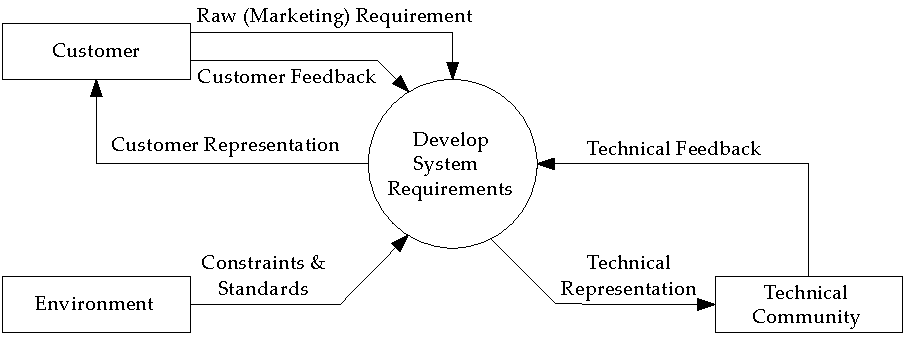
\includegraphics[width=4.6in,height=1.7in]{image1.pdf}
\caption{Requirements Specification development processes
from IEEE Std. 1233-1998. The three input sources to the process are the
customer, environment, and technical community.}
\label{figure: ieeeRequirements}
\end{figure}

\section{Engineering Requirements}
\label{section:engineering-requirements}

Before developing the complete Requirements Specification, designers
need to first determine individual engineering requirements.
\emph{\textbf{Engineering requirements}} are short statements that
address a technical need of the design. A simple example is ``\emph{The
system should be able to supply 50 watts of power.}'' This section
identifies the desirable properties of engineering requirements, methods
of identifying requirements, and provides numerous examples.

\subsection{Properties of an Engineering Requirement}
\label{section:properties-of-an-engineering-requirement}

Each engineering requirement should meet the four properties below
{[}IEEE Std. 1233-1998{]}:

\begin{enumerate}
\def\labelenumi{\arabic{enumi})}
\item
  \emph{Abstract.} This means that a given requirement should specify
  \emph{what} the system will do, not \emph{how} it will be implemented.
  This is the chicken and egg problem described earlier. It is
  frequently the most difficult property to satisfy since designers
  often have a preconceived concept for the solution. Unless absolutely
  necessary, the requirements should say nothing about the
  implementation. For example, a requirement stating that a certain
  microcontroller (i.e., technology) \ul{will} be used should be
  avoided. Admittedly, this is not always possible due to customer
  constraints or in cases where a system is being built upon
  pre-existing technology. A common analogy used for the ``\emph{what
  versus how}'' problem is that of designing a bridge. The requirement
  is to transport people from one side to other, without specifically
  stating the solution is a bridge, because another solution, like a
  ferry, may be a much more effective solution.
\item
  \emph{Verifiable.} Verifiability means that there should be a way to
  measure or demonstrate that the requirement is met in the final system
  realization. Doing so allows the system to be tested or verified
  against the requirements. The idea is that if there is no way to
  verify that the requirement is met, then it should not be a
  requirement. Verifiability is used to answer the question of
  ``\emph{Are we building the system correctly?}''
\item
  \emph{Unambiguous.} Each requirement should have a single unambiguous
  meaning and be stated with short complete sentences.
\item
  \emph{Traceable.} Requirements should be traceable marketing
  requirements. If the design doesn't satisfy the customer's needs, it
  won't be successful.
\end{enumerate}

Let's examine an example requirement for a robot whose objective is to
navigate autonomously within a specified environment. Consider the
following requirement

\begin{itquote}
The robot must have an average forward speed of 0.5 feet/sec, a top
speed of at least one foot/sec, and the ability to accelerate from
standstill to the average speed in under one second.
\end{itquote}

Are the four properties for an engineering requirement met? In terms of
the abstractness property, the answer is yes; it states what the system
must do, not how it will be implemented. In terms of the second
property, can the requirement be verified? Speed and acceleration are
directly testable in the final realization, and thus it is verifiable.
Is it unambiguous? It gives clear bounds for speed and acceleration.
Finally, traceability can't be shown without the marketing requirements
and is addressed later.

Now we analyze a second example requirement for the robot to see if it
meets the properties

\begin{itquote}
The robot must employ IR sensors to sense its external environment and
navigate autonomously with a battery life of one hour.
\end{itquote}

This requirement is not abstract since it identifies part of the
solution in terms of the sensor type and the fact that batteries must be
used. It is somewhat ambiguous in that it should specify what is meant
in terms of autonomous and the operating period. In terms of operating
period, should it work for exactly one hour and stop, or is greater than
an hour acceptable? Again, traceability can't be demonstrated without
the marketing requirements. This requirement would be hard to verify
without a good definition of what autonomous navigation in this context
means. A better requirement would be

\begin{itquote}
The robot must navigate autonomously, with the aid of only landmarks in
the specified environment, for a period of least one hour.
\end{itquote}

Realize that good requirements typically have two key elements in the
statement -- a description capability and condition. Capability
describes what the system must do and in the above requirement, that
capability is autonomous navigation. Conditions are measurable or
testable attributes of the capability and are critical for verification.


\subsection{A Fifth Property -- Realism}
\label{section:a-fifth-property-realism}

In addition to meeting the four properties, requirements should be
realistic or justified. This is not defined in the IEEE standard as a
property, but it is an important aspect that is often overlooked. To be
realistic, there should be a way of demonstrating that the target is
technically feasible. For example, a requirement could indicate that a
robot to should travel at a speed of 1,000,000 miles per hour, which
could be verifiable, unambiguous, and abstract -- yet, completely
unachievable. Realistic targets can be determined with a little
research, engineering know-how, creativity, or system modeling. One way
to do this is to assume a solution for the final system -- violating the
abstractness property. For example, consider the design of a robot where
some basic assumptions are made on the weight of the robot, the motors
used, the wheel size, and the battery selected. An engineering model
based upon these characteristics could be developed to predict
performance and estimate realistic requirements. Alternatively, target
requirements can be based upon an actual prototype, where a model or
experimental system is developed to show that a particular requirement
is feasible. This is how the technical community in 
Figure~\ref{figure: ieeeRequirements}
feeds into the requirements process.

The use of benchmarking to identify similar systems and their
performance provides a reference for realistic targets. It is generally
hard to surpass the performance of well-developed products and systems
on a first-generation design. An exception is with new and innovative
approaches that allow you to surpass the competition. Competitive
benchmarks may also be obtained from similar, but not necessarily
identical, products. Experience working with a particular technology or
previous generations of a system also provides guidance in selecting
realistic targets. That being said, organizations wishing to gain or
maintain a market edge often press the development team to achieve
performance on new generations that were once believed to be
unrealistic. Sometimes it just may not be feasible to determine the
technical feasibility of requirements. In such cases, the requirements
should have a certain amount of tolerance built into them and be updated
as development proceeds.

\subsection{Constraints}
\label{section:constraints}

One of the inputs to the requirements process in Figure~\ref{figure: ieeeRequirements}
is the environment, serving as the source of both constraints and standards. In
reality, all engineering requirements impose some sort of constraint on
a design, but in design a constraint is a special type of requirement. A
\emph{\textbf{constraint}} is a design decision imposed by the
environment or a stakeholder that impacts or limits the design.
Constraint requirements often violate the abstractness property. For
example, a constraint requirement is

\begin{itquote}
The system must use a PIC18F52 microcontroller to implement
processing functions.
\end{itquote}

This constraint requirement specifies how the system will be
implemented. This could be because the project sponsor has developed a
great deal of expertise using this particular microcontroller and does
not want to spend the development time learning a new platform. Note
that a number of other references define constraints to be synonymous
with non-functional requirements (usually indicated as items that are
not specifically functions). However, that terminology is avoided here
since it is not well defined nor universally accepted.

\subsection{Standards}
\label{section:standards}

\emph{\textbf{Standards}} are exactly what the name implies, a standard
or established way of doing things that ensure interoperability. Without
standards, the use of technology would be severely limited, if not
downright impossible. Standards ensure that products work together, from
home plumbing fixtures to the modules in a modern computer. Imagine if
every computer manufacturer had their own communication standard,
instead of following established protocols such as RS-232, TCP/IP, and
USB---computers would have a hard time printing, sending email, instant
messaging, or surfing the Internet! Furthermore, standards ensure the
health and safety of products that people use every day. Identifying and
following standards is an expected part of good engineering practice.

The focus in this chapter is on identifying standards that impact the
requirements and ultimately the design. The question becomes, what
standards are relevant to your project and how do you use them? There
are different levels of interaction with standards that we denote as:
user, implementation, and development levels. At the \emph{user level},
the standards are simply employed in the design, and detailed technical
knowledge of the standard is typically not necessary. For example, when
using a component that communicates to other devices, it is likely that
a standard communication protocol is used. Other than having to
configure software or hardware to communicate with the standard,
detailed knowledge of the standard isn't required. Another example would
be in developing software to display digital images in a standardized
format such as JPEG-2000 (Joint Photo Experts Group), in which case it
is likely that existing software components would be used to read and
display data in this format.

At the \emph{implementation level} details of the standard need to be
understood. Standards at the implementation level are most likely to
impact the design and the requirements. For example, when developing
low-level drivers for computer peripherals, you need to become an expert
on the underlying standard. Another example is reliability, where the
requirement may be that ``\emph{the system will have a reliability of
95\% in 10 years.}'' In this case a reliability standard, such as
\ul{Military Handbook for Reliability Prediction of Equipment}
{[}MIL-HDBK 217F{]} may be employed, and its usage requires an
understanding of both the reliability theory and the standard itself.

New standards are constantly being developed and existing ones modified,
leading to the final level of interaction at the \emph{development
level}. Depending upon the standard, engineers from different
organizations, professional societies, and corporations take part in the
standards setting process. Many participants in this process are trying
to gain a competitive advantage for their products and services.

It can be difficult to navigate the world of standards; they tend to be
highly detailed and limited parts of a standard may apply to a project.
In addition, many standards are costly to obtain, while some are freely
distributed. The following is advice for identifying and employing
standards. First, conduct research on applicable standards. Virtually
all standards organizations maintain websites that provide basic
information on their particular standards. The IEEE Xplore database is a
good place to start since it has a wide variety of standards and
provides free searchable abstracts. Many companies and universities have
subscriptions databases of complete standards. Second, determine the
expected level of interaction. Based upon your analysis of the problem,
do you foresee applying standards? Or will you need to develop an
in-depth knowledge at the implementation level? In the latter case, you
need to obtain detailed information on the applicable standards.
Finally, you should consider asking your client. They may have their own
internal standards and procedures to follow, and they may have experts
on the applicable standards.

The list below identifies some of the types of standards that may be
employed in a project and included in the requirements.

\begin{itemize}
\item
  \emph{Safety}. Safety standards address how to design for safety and
  how to test products to ensure that they are safe.
\item
  \emph{Testing}. Testing standards are often related to safety, but are
  broader in scope. For example, standardized benchmark tests are used
  for comparing computational performance, one well-known standard being
  the SPEC (Standard Performance Evaluation Corporation) benchmarks.
\item
  \emph{Reliability}. Reliability standards address general reliability
  principles and design methods for different classes of systems.
  Another practical aspect is in the estimation of reliability of
  electronic systems, such as the IEEE and military reliability
  standards.
\item
  \emph{Communications.} They address how electronic systems communicate
  and transfer information, such as in computing, telephony, and
  satellite communications.
\item
  \emph{Data Formats}. Standard data formats ensure that systems and
  software can properly share information. Examples include image,
  video, and database standards.
\item
  \emph{Documentation}. There are standards for technical report
  documentation. In addition, there are standards for documenting
  processes and business practices, a well-known case being the ISO
  (International Standards Organization) 9000 and subsequent standards.
\item
  \emph{Design Methods.} Certain design techniques are standardized as
  well. Examples include software design methodologies, and the use of
  design languages such as the Hardware Description Language (HDL) and
  the Unified Modeling Language (UML).
\item
  \emph{Programming Languages.} Programming language syntax is
  standardized so that software maintains a level of portability between
  systems and compilers.
\item
  \emph{Connector Standards.} Standards for cable connections are common
  and should be followed to ensure that systems are easily interfaced
  and manufactured.
\item
  \emph{Meta-Standards.} Some standards are a combination of multiple
  standards known as meta-standards. For example, the RS-232 standard is
  really a combination of a mechanical standard describing the connector
  physical dimensions connector, an electrical standard describing the
  voltages, a functional standard describing the pins and their
  function, and a procedural standard describing how entities
  communicate.
\end{itemize}

\subsection{Identifying Engineering Requirements}
\label{section:identifying-engineering-requirements}

There are many techniques for identifying requirements listed below
{[}IEEE Std. 1233-1998{]}:

\begin{itemize}
\item
  Structured workshops and brainstorming sessions.
\item
  Interviews, surveys, and questionnaires.
\item
  Observation of processes or devices in use.
\item
  Competitive benchmarking and market analysis.
\item
  Prototyping and simulations.
\item
  Research and technical documentation review.
\end{itemize}

Many requirements may be specified for a design, but knowing which to
include is the challenge. The remainder of this section is a guide to
describe the types of engineering requirements that may be specified for
electrical and computer systems. Requirements in categories of
performance and functionality are presented first as they are often
critical, followed by an alphabetical grouping of a potpourri of other
types requirements. \textbf{This taxonomy of requirements is by no means
definitive or inclusive of all possibilities, and the design team needs
to carefully determine those that are applicable to the particular
situation. Careful attention must be given to the verifiability of
requirements for the particular application.}

\subsection*{Performance}
\label{subsection:performance}

These requirements reflect a critical aspect of the performance of the
system or device. They often are characterized by time, accuracy,
throughput, or percentage error. The following is an example requirement
that might be used in a security application with camera surveillance.

\begin{itquote}
The system should detect 90\% of all human faces in an image.
\end{itquote}

In order to verify this, a test might be constructed where the system is
presented with a large database of face images that the system was not
developed or trained with. The number of faces correctly detected would
then be determined. Here is another example performance requirement for
a system that measure part location

\begin{itquote}
The system should be able to measure part location to within ± 1mm.
\end{itquote}

One way to verify this would be to take independent measurements of the
system's ability to measure part location and compare them to the result
of the system. The following is an example that could apply to software
response time.

\begin{itquote}
The system should retrieve the user data no less than three seconds for
90\% of requests and in a maximum of six seconds for all requests.
\end{itquote}

This could be verified by constructing a test where a large number of
queries for user data are presented to the software under a variety of
operating conditions and the response time measured. Yet another example
is:
\begin{itquote}
The system should be able to process video data at a rate of 30 frames
per second.
\end{itquote}

This could be verified by providing an input video stream at the frame
rate and testing to ensure that proper processing occurs. The test
procedure would need to specify length and number of videos to test,
issues that are addressed in Chapter 7. A final example of performance
is one that could apply to electrical audio amplification

\begin{itquote}
The amplifier will have total harmonic distortion of less than 1\%.
\end{itquote}

Total harmonic distortion is a measure that quantifies how closely an
amplifier is able to replicate the original signal. This would likely be
verified using laboratory instrumentation to measure the harmonic
distortion in the output signal.


\subsection*{Functionality}
\label{subsection:functionality}

These requirements describe the type of functions that a system should
perform. Often, they provide inputs, outputs, and the transformation
that the system will perform on the inputs. This is examined further in
Chapter 5, which presents functional design techniques. The following is
an example, where the input is ambient air temperature is converted to a
digital readout. It also has a performance aspect in that the accuracy
is specified.

\begin{itquote}
The system will convert ambient temperature to a digital readout of
temperature with an accuracy of 1\% over the measurement range.
\end{itquote}

The following is an example from a real capstone project to develop a
wireless mouse that is worn by the user and integrated into a glove.

\begin{itquote}
The system will implement the left and right button functions of a
standard mouse.
\end{itquote}

The following are several functional examples for software systems.

\begin{itquote}
The user shall be able to search all five company internal databases. \\ \\
The system will protect the user's identity with 128-bit encryption.
\end{itquote}

Note that in these last two cases, verification would be by inspection.


\subsection*{Economic}
\label{subsection:economic}

Economic requirements include the costs associated with the development
(design, production, maintenance) and sale of a system. They may also
include the economic impact of the final system, such as how it will to
contribute to profits or save the user money. Two example economic
requirements are below.

\begin{itquote}
The costs for developing the system (labor and parts) should not exceed
\$50,000. \\ \\
The total parts and manufacturing costs cannot exceed \$500 per unit.
\end{itquote}

\subsection*{Energy}
\label{subsection:energy}

Virtually all systems consume and/or produce energy and thus have energy
requirements. Energy consumption is the amount of power that a system
consumes, and may be specified in terms of maximum, minimum, or average
values. Example requirements are

\begin{itquote}
The system will have an average power consumption of 500mW. \\ \\
The system will have a peak current draw of 1A.
\end{itquote}

These requirements could be verified by measuring current and voltage
draws under the different operating conditions, or by estimating the
power drawn by all components in the system.


Operating lifetime addresses how long the system will operate from a
given power source. For battery-powered devices, operating time is
critical, and the lifetime for a given source may be an important
requirement. An example of such a requirement is

\begin{itquote}
The system will operate for a minimum of three hours without needing to
be recharged.
\end{itquote}

Source characteristics refer to the characteristics of the input and/or
output sources, such as voltage, current, impedance, frequency, number
of phases, and power requirements. An example requirement is

\begin{itquote}
The system will operate from a 12V source that supplies a maximum
current of 300mA.
\end{itquote}

\subsection*{Environmental}
\label{subsection:environmental}

These requirements address the impact of the design on the external
environment and usage of the earth's resources. For example, energy
usage is an important factor and example requirement is as follows

\begin{itquote}
The system will use 20\% less energy than the industry average for
similar products and qualify for US Energy Star certification.
\end{itquote}

Recyclability is the ability to dismantle a product into its constituent
materials for reuse in other products. European countries have
regulations on the recyclability of consumer products. In many cases,
the producer of a product is responsible for its safe disposal once its
service life is over. An example requirement is as follows

\begin{itquote}
50\% of the modular components will be able to be repaired and re-used
in similar products.
\end{itquote}

\subsection*{Health and Safety}
\label{subsection:health-and-safety}

The health and safety of anyone affected by the final product is an
especially important consideration. For example, IEEE and ANSI standards
provide guidance on safe levels for exposure to radio frequency electric
fields.

\begin{itquote}
The system will not expose humans to unhealthy levels of
electromagnetic radiation and will meet conditions for safe operation
identified in ANSI Std. C95.1.
\end{itquote}

There is a tendency to think that physical harm is not an issue in
electrical and computer systems, but many electronic systems control
mechanically moving parts. Consider the design of an automatic garage
door system. An example constraint could be that

\begin{itquote}
The door should stop moving if a person or object is detected in the
door path.
\end{itquote}

This could also translate into further engineering requirements on the
amount of force on the door required to trigger it to stop. There are
many safety standards, and two that are widely applied for consumer
products are the UL (Underwriters Laboratory) and CE (Common European)
standards. Examples are

\begin{itquote}
The system will use only UL approved components.\\ \\
The final system will be meet UL and CE standards and be tested at an
independent laboratory for approval.
\end{itquote}

\subsection*{Legal}
\label{subsection:legal}

Designs should not infringe upon existing patents, copyrights, and
trademarks, particularly if the intention is to sell the product. Patent
searches should be conducted, and search capabilities are available at
the United States Patent Office website
(\href{http://www.uspto.gov}{www.uspto.gov}). An example is

\begin{itquote}
An intellectual property search will be conducted to ensure that there
is no infringement on prior patents.\\ \\
This could be verified by having an external firm will conduct the
patent search and evaluate the design against existing intellectual
property.
\end{itquote}

Security and privacy constraints apply to systems that handle sensitive
data or personal communications. The ability of computing systems to
withstand malicious attacks by hackers is another consideration, and the
use of firewalls or other protective measures may be warranted. Examples
are

\begin{itquote}
The system will protect the user's identity with 128-bit encryption as
required by law.
\end{itquote}

\subsection*{Maintainability}
\label{section:maintainability}

The maintenance of the system being developed and compatibility with
other systems are often considerations. Will the system be designed so
that it can be reused in future applications? This is common in software
development where the objective is to design modules that are reliable
and flexible enough to be used in other applications. It is also a
consideration in terms of the reusability of electronic or digital
components in future system upgrades. An example reuse constraint is

\begin{itquote}
The software should maintain downward capability and be able to use
version 2 object libraries.
\end{itquote}

After a product goes into service, it enters the maintenance phase,
where it is maintained and upgraded. In software designs this is an
important consideration, as software is regularly upgraded and
maintained. On the hardware side, maintenance can be facilitated by the
use of plug-in modules that are easily removed and replaced. Examples
are

\begin{itquote}
The system will initially be available to 100 users at five field
locations, and within one year must be expanded to address usage by
5,000 users company-wide.\\ \\
The system should have a modular design such that failed components can
be replaced by a technician in under 15 minutes.
\end{itquote}

There may be internal restrictions on system development imposed by the
company based on their internal expertise and ability to maintain the
system, such as the following constraint requirement.

\begin{itquote}
The system will use only PIC microcontrollers.
\end{itquote}

\subsubsection*{Manufacturability}
\label{subsection:manufacturability}

A prevalent product development paradigm that used to be employed in
many engineering organizations was to ``\emph{throw the design over the
wall}.'' What this meant is that the design and development team would
create a new product and hand it off to the manufacturing team to
produce (throw it over the wall and run), often without having
considered the manufacturability of the product. The manufacturing team
would then address how to produce the design, and in many cases could
not do so without major redesign. Fortunately, this has given way to
much better concurrent engineering practices where all aspects of
product development are considered throughout the process. All of the
examples presented here are constraints, in that that they are external
decisions that limit the design.

Size is a consideration in terms of the amount of space the final design
will occupy, particularly if it has to be physically integrated with
other components. An example constraint requirement is

\begin{itquote}
The system must be manufactured on a circuit board with dimensions of no
greater than 1''x2''.
\end{itquote}

The realization and portability of the system is a consideration. For
example, with electronics, will it be built on a printed circuit board?
Following design rules and file format guidelines is important for
manufacturing printed circuit boards and integrated circuits. A chip
foundry may require that integrated circuit layouts utilize certain file
formats. Examples are below, which again are clear constraints on the
design.

\begin{itquote}
The system will be manufactured using three layer printed circuit board
technology.\\ \\
The product should be run on the Linux operating system.
\end{itquote}

The use of readily available parts, instead of low volume or hard to
find components, improves manufacturability, and an example is

\begin{itquote}
The design shall only incorporate components that can be purchased
through two of our main suppliers.
\end{itquote}

\subsubsection*{Operational}
\label{subsection:operational}

Operational requirements address the physical environment in which the
system will operate. Characteristics could be temperature, humidity,
electromagnetic radiation, shock, and vibration. Note, that these can
often be quite difficult to verify and may require specialized equipment
to do so. An example temperature operational requirement is

\begin{itquote}
The system should be able to operate in the temperature range of 0°C to
75°C.
\end{itquote}

This could be tested via test in an environmental chamber which the
operation of the system is tested over the complete temperature range.
Alternatively, indirect verification is a possibility. For example, in
the design, only components that are known to meet this operational
requirement, as specified in their product datasheet, could be used.


Depending upon the customer needs, the system may be tested in an
environmental chamber to verify that the requirement is met. Humidity is
similar in concept to the temperature requirement, addressing the
required ambient humidity range. A system may also need to be
water-resistant (withstand rain and snow) or waterproof (be submersible
in water). An example requirement is

\begin{itquote}
The system must be waterproof and operate while submersed in water.
\end{itquote}

Be careful with the differences between waterproof (submersible in
water) and water-resistant, which indicates the ability to withstand
outdoor elements such as rain and snow. For example, outdoor decorative
lights are water-resistant, but not waterproof.


Depending upon the environment, the system may need to withstand
vibrations. Bounds are typically specified in terms of frequency,
magnitude, and duration of the vibration. An example requirement is

\begin{itquote}
The system must be able to withstand vibrations of up to 60Hz with a
peak magnitude of 1mm for a period of 1 minute.
\end{itquote}

Electromagnetic Interference \emph{(EMI)} results from any
electromagnetic energy that interferes or disturbs the operation of an
electronic system. Electronic systems may produce electromagnetic
radiation and limits may need to be placed upon the amount of radiation
emitted. EMI is typically measured with specialized testing apparatus.
Conversely, a system may need to be able to operate properly given a
certain level of EMI.

The system may need to withstand a specified amount of shock and still
operate. This may be measured in G-force or via heuristics. An example
requirement is

\begin{itquote}
The system should withstand a drop from a height of six feet and still
operate.
\end{itquote}

\subsubsection*{Political}
\label{subsection:political}

Political constraints address relationships to political, governmental,
or union organizations. Examples include obtaining governmental
approvals, resolving trade barriers, and determining the acceptance of
systems for use in unionized environments. Examples are below.

\begin{itquote}
The system will need to obtain FDA approval before it can be sold to
medical users.\\ \\
The software will comply with the Digital Millennium Copyright Act.
\end{itquote}

\subsubsection*{Reliability and Availability}
\label{subsection:reliability-and-availability}

This refers to the expected period of time that a system will operate
properly. Measures of r\emph{eliability} include failure rates and mean
time to failure. Estimation of system reliability is given detailed
coverage in Chapter 8. The following is an example of a reliability
requirement.

\begin{itquote}
The system will have a reliability of 95\% in five years.
\end{itquote}

This requirement means that 95\% of the systems should be properly
operating (have not failed) in five years. Direct measurement of
reliability would not be possible, unless you are willing to wait five
years to see how many systems fail, thus the use of estimation. This
would require indirect verification using mathematical techniques to
estimate the system reliability.

\emph{Availability} is related to reliability, but addresses the amount
of time that a system is available for operation. Example availability
requirements are

\begin{itquote}
The system will be operational 99\% of the time.\\ \\
The system will be operational from 4AM to 10PM, 365 days a year.
\end{itquote}

These might be hard to verify this since it is only determined for sure
once the system is deployed. Verification would have to address under
which conditions the system would be tested to ensure this occurs.


\subsubsection*{Social and Cultural}
\label{subsection:social-and-cultural}

This addresses aspects such as benefits, risks, and acceptance of
products by the intended user or by society at large. For example,
robots have tremendous benefits for improving product quality, while
freeing people from dangerous and repetitive tasks. Yet when used in
automation, they present the risk of displacing workers and causing job
losses.

Many great products have fallen by the wayside because users were
unwilling to accept it. An example is the early Apple Newton Personal
Digital Assistant, the first product of its kind. The fatal flaw was
handwriting recognition that required a training process for accurate
recognition. This was not accepted by consumers and
Palm\textsuperscript{®} Computing solved the problem by employing a
simplified alphabet known as Graffiti. Graffiti was also seen as risky
when it was being developed, but due to its simplicity it was accepted
by consumers and the product became a huge success. In the mid 1980s,
Phillips electronics released the Laser Disk player, which failed
magnificently, but was far superior to VHS technology. Their failure was
attributed to the cost of the players and disks when compared to VHS.
Fifteen years later DVDs, with the help of computers, reached a price
point which now makes them preferable to VHS.

Will the system be used by engineers, technicians, laborers, doctors,
lawyers, or the general public? Each group has its own culture,
educational background, and willingness to accept innovations. Example
requirements are

\begin{itquote}
The product shall provide help menus to the user in either English or
Spanish. \\ \\
The software will be designed to easily be used by operators on the
manufacturing floor. The software will be tested by a group of 25
operators and the average time to learn the basic functionality of the
software will not exceed 8 hours.
\end{itquote}

\subsubsection*{Usability }
\label{subsection:usability}

\emph{Usability requirements} address the ease of use of a system.
Although they are quite common, they are often difficult to verify.
Usability can address how long it takes to learn the product and
satisfaction by the end-user or a group of users. To aid in verification
conditions can be placed on the number of menus in the system, an
estimated learning time, and number and types of errors the user is
allowed to make. An example requirement is that

\begin{itquote}
Users of the system should be able to learn 80\% of its functionality
within two hours.
\end{itquote}

The method of verification would need to be clearly specified, such as,
a group of 25 test users who have never used the product will be
provided two hours to learn the product. Another example of a usability
requirement is

\begin{itquote}
The system will have a maximum of 20 functions and a maximum of two
menus of depth.
\end{itquote}

\section{Developing the Requirements Specification}
\label{section:developing-the-requirements-specification}

The Requirements Specification is the complete set of all system
requirements. The steps in developing the Requirements Specification are
to:

\begin{itemize}
\item
  Identify requirements from the customer, environment, and the
  technical community (focus of the previous section).
\item
  Ensure the engineering requirements are well-formed (meet the
  properties).
\item
  Organize the requirements. Similar requirements should be presented
  together and relationships between engineering and marketing
  requirements identified. The collection of requirements should meet
  the properties identified in this section.
\item
  Validate the Requirements Specification -- which means all
  requirements are examined to ensure they meet the needs of the
  stakeholders.
\end{itemize}

\subsection{Properties of the Requirements Specification}
\label{subsection:properties-of-the-requirements-specification}

The desirable properties of the Requirements Specification are as
follows {[}IEEE Std.1233-1998{]}:

\begin{enumerate}
\def\labelenumi{\arabic{enumi})}
\item
  \emph{Normalized (orthogonal) set}. There should be no overlap or
  redundancy between engineering requirements. A mathematical analogy is
  that of orthogonal vectors. For example, the x and y axes of the
  two-dimensional Cartesian space are orthogonal vectors, meaning that
  the projection (dot product) of one vector onto the other is zero.
  Ideally, all requirements should be orthogonal with no redundancy.
\item
  \emph{Complete set.} A complete Requirements Specification addresses
  all of the needs of the end-user and also those needs required for
  system implementation. Failure to define a complete set results in
  \emph{\textbf{under-specificity}} where not all needs are met.
\item
  \emph{Consistent}. The engineering requirements should not be
  self-contradictory.
\item
  \emph{Bounded.} The scope of the Requirements Specification should be
  identified. Determine the minimum acceptable bound for target values;
  going beyond what is necessary limits the design space of potential
  solutions. Applying unnecessary bounds results in
  \emph{\textbf{over-specificity}}.
\item
  \emph{Modifiable.} Requirements are typically considered to be
  evolutionary. This is because there are many unknowns at the start of
  a project, hence estimates for the requirements are made. The original
  requirements are known as \emph{\textbf{baseline requirements}}. The
  estimates can change as development proceeds, as long as the changes
  are communicated to and agreed upon by all affected parties. Versions
  of the requirements should be tracked and identified as modifications
  take place.
\end{enumerate}

\subsection{Requirements Validation}
\label{subsection:requirements-validation}

An important property of an engineering requirement that we saw earlier
was verifiability. Verifiability seeks to answer the question of whether
or not the system is being developed correctly, or \emph{``Are we
building the product correctly?''} A related concept is that of
validation, which seeks to answer the question ``\emph{Are we building
the correct product?}'' More formally, \emph{\textbf{validation}} is the
process of determining whether the system meets the needs of the
user---is it valid? This is more general in scope than verification and
more difficult to show. Requirements validation is usually carried out
by reviews of the requirements by a team of people. Validation is
demonstrated by being able to answer the following questions in the
affirmative {[}Som01{]}:

\begin{itemize}
\item
  For each individual engineering requirement, are the traceability and
  verifiability properties met? Is each requirement realistic and
  technically feasible?
\item
  For the Requirements Specification, are the properties of
  orthogonality, completeness, and consistency met?
\end{itemize}

  A complete Requirements Specification includes all the requirements,
  both marketing and engineering, along with the relationships between
  them. The relationships between the engineering and marketing
  requirements need to be described to ensure that all the marketing
  requirements are being addressed by design. The relationship between
  the marketing and engineering requirements is called a mapping
  because, like a mathematical mapping, it defines which elements of the
  domain (marketing requirements) are associated with which elements of
  the range (engineering requirements).


\section{Requirements Case Studies}
\label{section:requirements-case-studies}

This section presents case study examples of Requirements Specification,
most of which are from real capstone design projects. They are presented
in a table format that presents each engineering requirement, the mapped
marketing requirements (supporting the traceability property), and the
justification for each requirement. The marketing requirements are
summarized at the end of the table.

\subsection{Case Study: Car Audio Amplifier}
\label{subsection:case-study-car-audio-amplifier}

Table~\ref{table:audioRequireSpec} presents the Requirements Specification for a car audio
amplifier. This simple example was selected because of the relative ease
of understanding, broad familiarity with this type of device, and it
will be expanded upon later.

\begin{table}
\centering
\caption{Requirements Specification for an audio amplifier for
use in an automobile.}
\label{table:audioRequireSpec}
\begin{tabular}{ |p{2cm}|p{5cm}|p{5cm}|} 
\hline
\rowcolor{Gray}
\textbf{Marketing Requirements} & \textbf{Engineering Requirements} & \textbf{Justification} \\ \hline
                           
1, 2, 4 &
1.  The \emph{total harmonic distortion} should be \textless0.1\%. &
Based upon competitive benchmarking and existing
amplifier technology. Class A, B, and AB amplifiers are able to obtain
this level of THD. \\ \hline

1--4 & 
2.   Should be able to sustain an \emph{output power} that averages $\ge 35$
  watts with a peak value of $\ge 70$ watts. & 
This power range provides more than adequate sound
throughout the automobile compartment. It is a sustainable output power
for projected amplifier complexity. \\ \hline

2, 4 & 
3. Should have an efficiency $\eta > 40\%$. &
Achievable with several different classes of power amplifiers. \\ \hline

3 & 
4.   \emph{Average installation time} for the power and audio connections
  should not exceed 5 minutes. &
Past trials using standard audio and power jacks
demonstrate that this is a reasonable installation time. \\ \hline

1--4 & 
5.  The \emph{dimensions} should not exceed 6'' x 8''x 3''. &
Fits under a typical car seat. Prior models and
estimates show that all components should fit within this package
size. \\ \hline

1--4 & 
6.  \emph{Production cost} should not exceed \$100. &
This is based upon competitive market analysis and previous system designs. \\ \hline

\multicolumn{3}{|p{12cm}|}{
\textbf{Marketing Requirements}\newline
1.  The system should have excellent sound quality.\newline
2.  The system should have high output power.\newline
3.  The system should be easy to install.\newline
4.   The system should have low cost.
} \\ \hline
\end{tabular}
\end{table}

Audio power amplifiers are widely available devices, so the requirements
were determined through competitive benchmarks and knowledge of
amplifier circuit designs. The first engineering requirement directly
impacts sound quality and is known as total harmonic distortion (THD).
THD measures how closely the amplifier output signal follows the input
signal. It is desirable for an amplifier to have a linear relation
between input and output, where the output signal is identical to the
input signal, except for an amplification factor. In reality, all
amplifiers have some degree of nonlinearity or distortion. It is
measured by applying a pure sinusoid as the input to the amplifier,
which in the case of a perfectly linear amplifier produces a pure output
sinusoid of the same frequency. Any nonlinearity introduces unwanted
harmonic frequencies. THD represents the power of unwanted harmonics
relative to the power of the fundamental sinusoid. THD is typically less
than 1\% for a good amplifier.

The second requirement, output power, is quantified in terms of both
average and maximum values to minimize ambiguity. The third engineering
requirement addresses the efficiency of the power transfer, or how much
of the power consumed by the device is actually converted to audio
power. The fourth engineering requirement, ease of installation, is
perhaps easy to understand intuitively, and the expected installation
time provides the condition for verification. The fifth requirement
addresses the physical size of the device, and is important as it will
need to be installed somewhere in the vehicle.

\subsection{Case Study: iPod\textsuperscript{TM} Hands-Free Device}
\label{subsection:case-study-ipodtm-hands-free-device}

Table~\ref{table:ipod} presents the Requirements Specification for a hands-free
device whose intent is to allow a driver to communicate with an
iPod\textsuperscript{TM} audio player while driving. The Problem
Statement was presented in Chapter 2 (Section 2.6).

\begin{table}
\centering
\caption{Requirements Specification for the
iPod\textsuperscript{TM} Hands-Free Device.}
\label{table:ipod}

\begin{tabular}{ |p{2cm}|p{5cm}|p{5cm}|} 
\hline
\rowcolor{Gray}
\textbf{Marketing Requirements} & \textbf{Engineering Requirements} & \textbf{Justification} \\ \hline

4, 6 & 
1.  System will i\emph{mplement nine voice command} functions ( menu,
  play/pause, previous, next, up, down, left, right and select) and
  respond appropriately according to each command. &
  hese are the basic nine commands that are used to
control an iPod and will provide all functionality needed. \\ \hline

1, 3, 4, 7 & 
2.   The \emph{time to respond} to voice commands and provide audio
  feedback should not exceed 3 seconds. &
The system needs to provide convenient use by
responding to the user inputs within a short time period. Based on
research it was determined that the response time for the iPod is less
than 1 second and an average voice recognition system requires 2 seconds
to recognize commands. \\ \hline

4, 6 & 
3.   The \emph{accuracy} of the system in accepting voice commands will be
  between 95\% and 98\%. &
Research demonstrates that this is a typical accuracy
of voice recognition chips. Speaker independent systems can achieve 95\%
and speaker-dependent up to 98\%. \\ \hline

5, 6 & 
4.   The system should be able to \emph{operate} from a 12 V source and
  will draw a maximum of 150 mA. &
The automobile provides 12V DC. A current draw budget
estimate was developed with potential components and 150mA was an upper
limit of current estimated. \\ \hline

5, 6, 7 & 
5.  The \emph{dimensions} of the prototype should not exceed 6'' x 4'' x  1.5''. &
This system must be able to fit in a car compartment,
somewhere between the seats. Estimate is based upon a size budget
calculation using typical parts. \\ \hline

\multicolumn{3}{|p{12cm}|}{
\textbf{Marketing Requirements}\newline
1. Should not minimize or slow down the functional quality of the iPod.\newline
2.  User should be able to search for songs and artists and receive feedback on selection.\newline
3.  System should provide clear understandable speech.\newline
4.  System should be able to understand voice commands from user.\newline
5.  Should be able to fit and operate in an automobile.\newline
6.  Should be easy to use.\newline
7.  Should be portable.
} \\ \hline
\end{tabular}
\end{table}

To develop the marketing requirements, this team conducted an informal
survey of students on campus, asking the target group what their desires
for such a system would be. The first three engineering requirements are
related to the important issues of the system functionality and
performance. In order to develop justifications for some of the
requirements a prototype solution had to considered, although the
solution has not been formally posed. For example, in order to estimate
a time for responding to a user's command, some assumptions were made on
the types of components that might be used in the design. The last two
requirements are operational requirements, ensuring that the device will
work in its intended environment.

\subsection{Case Study: Gigabit Ethernet Card Testing}
\label{subsection:case-study-gigabit-ethernet-card-testing}

Table~\ref{table:gigabit} presents an example Requirements Specification developed for
the design of an experimental test setup {[}Ese03{]}. The Problem
Statement for this example was presented in Chapter 2, where the
objective was to design a system to test a gigabit Ethernet card for use
in a harsh operating environment. In particular, the effects of
temperature and vibration variations on the optical power margin, both
of which impact the bit-error rate and the system performance, were
determined.

\begin{table}
\centering
\caption{System Requirements for a Gigabit Ethernet card
testing project.}
\label{table:gigabit}

\begin{tabular}{ |p{2cm}|p{5cm}|p{5cm}|} 
\hline
\rowcolor{Gray}
\textbf{Marketing Requirements} & \textbf{Engineering Requirements} & \textbf{Justification} \\ \hline

1 & Must be able to measure the \emph{optical power output} with an
\emph{accuracy} of ± 0.5dB. & This is based upon commercially available
optical power measurement instruments. \\ \hline
2 & Must be able to measure the \emph{optical power output} from 10°C to
55°C. & This range simulates the operating environment, and 55°C is the
maximum operating temperature of the card. \\ \hline
2 & The system must maintain \emph{temperature accuracy} to within ± 1°C
during all tests. & Based upon accuracy of commercially available test
chambers. \\ \hline
3 & Must be able to measure optical power over a \emph{frequency range}
from 4Hz to 33Hz in increments of 1Hz. & The frequencies encountered in
actual operation will not exceed this range. \\ \hline
3 & The \emph{peak vibration amplitude} should be 0.01 inches. & The
amplitude in the operating environment will not exceed this value. \\ \hline
3 & The card should be tested at a given frequency for a \emph{duration}
of 1 minute. & This exceeds the expected duration of vibration at given
frequency that the system will encounter. \\ \hline
3 & The vibration effects should be tested in x, y, and z
\emph{directions}. & The system will encounter vibrations in multiple
directions. This will provide data on differences in directional
variation due to vibration. \\ \hline
3 & The experiment should determine \emph{resonant frequency} to an
accuracy of ± 0.5Hz. & This will provide data on worst case vibration at
the resonant frequency. \\ \hline

\multicolumn{3}{|p{12cm}|}{
\textbf{Marketing Requirements} \newline
1.  The measurement of the optical power should be accurate.\newline
2.  It should measure the effects of temperature variations on optical power.\newline
3.  It should measure effects of vibration on the fiber optic connector
  and optical power output.}  \\ \hline
\end{tabular}
\end{table}

The marketing requirements were quite brief and direct, and not
surprising due to the fact the customer in this case was group of
engineers who had a good idea of what they wanted. The engineering
requirements were selected based upon characteristics of the operating
environment, through discussion with the engineers, and via some
educated guesswork. Let's consider some of the requirements, starting
with the effects of temperature variation on the optical power output.
The testing requirement on the temperature range was selected based on
the operating environment, while the accuracy is driven by the test
equipment. The requirements also address the vibration testing
requirements, including the vibration frequency range, amplitude, and
resonant frequency.

\subsection{Case Study: Portable Aerial Surveillance System}
\label{subsection:case-study-portable-aerial-surveillance-system}

The Requirements Specification for the Portable Aerial Surveillance
System (Problem Statement presented in Chapter 2) is shown in Table~\ref{table:portableAerial}.
This system is intended to provide police and emergency responders with
a low-cost easy to deploy aerial surveillance system.

\begin{table}
\centering
\caption{System Requirements for the Portable Aerial
Surveillance System.}
\label{table:portableAerial}

\begin{tabular}{ |p{2cm}|p{5cm}|p{5cm}|} 
\hline
\rowcolor{Gray}
\textbf{Marketing Requirements} & \textbf{Engineering Requirements} & \textbf{Justification} \\ \hline

6 & 
 System will provide visual recognition of license plate text from a
  minimum distance of 150 feet during daytime and nighttime use. &
   Recorded images and video will be used as trial
evidence. The device's maximum height is 150 feet, so
the device should allow text recognition at an absolute minimum of that
distance. The device must be also usable during nighttime.\\ \hline

4, 9 & 
   The device must be operable by a single person. &
 A police officer dispatched alone in his or her cruiser
should be able to launch and operate the device with no assistance. \\ \hline

2 & 
 This device must remain airborne for a minimum of two hours. &
Based upon interviews with law enforcement users. This
is a time period that covers most emergency situations. \\ \hline

7, 8 & 
 The device will be able to be used in at least 14 mph winds.&
 Device will be used outdoors and in non-ideal
conditions in Erie, PA, where there is a 95\% chance that winds will be
at or below 14 mph. \\ \hline

7 & 
  The device must not exceed a height of 150 feet above ground level
  when in use. &
  This device must comply with FAA regulation 101.15 \\ \hline
  
3 & 

  Must fit into the trunk of a police cruiser. The Chevrolet Impala has
  a trunk measuring 54 inches wide by 38 inches deep by 16 inches high. &
 Will be transported in a police cruiser and must fit
into the trunk of the vehicle. \\ \hline

1 & 
  The device will cost less than \$3000 per year to operate. &
 The budget allotted to Erie county police departments
was \$16.7 million. 0.85\% of Erie\textquotesingle s annual budget would
allow for \$140,280 to be used for a helicopter. A device having less
than 2\% of the annual operating costs of a helicopter, and having many
of the same surveillance capabilities would be considered a reasonable
expense. \\ \hline

\multicolumn{3}{|p{12cm}|}{
\textbf{Marketing Requirements}\newline
1.  The device should be able to be held stationary in the air, meaning
  providing enough stability to provide functionality.\newline
2.  Should be capable of being deployed for a long period of time.\newline
3.   Should be able to be deployed by one person in 3-5 minutes.\newline
4.  Should record video with enough quality to be used as evidence.\newline
5.  Should be useful at night.\newline
6.  Should fit in the trunk of a car and withstand the stresses of
  transportation.\newline
7.  Should be repairable and reusable.\newline
8.  Should require minimal training to be operated by one person.\newline
9.  Should be relatively inexpensive compared to that of a helicopter.\newline
10.  Should be able to operate at an altitude above most buildings.\newline
11.  Should meet any applicable governmental regulations (such as FAA).\newline
12.  Should be able to operate in typical winter conditions.}  \\ \hline
\end{tabular}
\end{table}

This project was developed in conjunction with Penn State Behrend and
the Mercyhurst College's Institute for Intelligence Studies to meet a
need that the institute identified. The student team met with a number
of law enforcement officials to determine the needs. The first
engineering requirement addresses the critical functionality that the
system is to provide, while engineering requirements 2--5 address the
performance and ability to work in the outdoor environment. Note the
inclusion of a federal standard that drives the requirement on the
maximum deployment height of the device. Requirement 7 addresses the
cost, which can often be difficult to justify in student projects, but
in this case the team has developed a clear justification.

\section{Advanced Requirements Analysis}
\label{section:advanced-requirements-analysis}

This section examines more advanced methods that are used to analyze and
refine requirements. There are tradeoffs between the different
requirements and understanding them is valuable for refining the
requirements themselves and developing solution concepts. This section
addresses tradeoffs between engineering and marketing requirements,
tradeoffs between engineering requirements themselves, and benchmarking.
At the conclusion, all of this is integrated in to the well-known House
of Quality.

\subsection{The Engineering-Marketing Tradeoff Matrix}
\label{subsection:the-engineering-marketing-tradeoff-matrix}

This matrix identifies how engineering and marketing requirements impact
each other. To demonstrate its construction, we continue to examine the
automobile audio amplifier example from Table~\ref{table:audioRequireSpec}. 
The tradeoff matrix
is shown in Table~\ref{table:engMarketingMatrix}, where the marketing 
requirements constitute the
row headings and the engineering requirements the column headings.

\begin{table}
\centering
\caption{Engineering-marketing tradeoff matrix for the audio
amplifier. ↑=positive correlation, ↑↑=strong positive correlation,
↓=negative correlation, ↓↓=strong negative correlation.}
\label{table:engMarketingMatrix}

\begin{tabular}{|l|l|l|l|l|l|l|l|} 
\hline
\rowcolor{Gray}
  &   & \rotatebox[origin=c]{90}{THD} & 
  			\rotatebox[origin=c]{90}{Output Power} & 
  			\rotatebox[origin=c]{90}{$\eta$, Efficiency} & 
  			\rotatebox[origin=c]{90}{Install Time} & 
  			\rotatebox[origin=c]{90}{Dimensions} & 
  			\rotatebox[origin=c]{90}{Cost} \\ \hline
  
  \rowcolor{Gray}
  &   &  -      &  +                     & +               & -                   & -                    &  - \\ \hline

1) Sound Quality & + & ↑↑ & ↓ & & & ↓↓ & ↓↓ \\ \hline
2) High Power & + & ↓ & ↑↑ & ↑ & & ↓↓ & ↓ \\ \hline
3) Install Ease & + & & ↓ & & ↑↑ & ↑ & ↓ \\ \hline
4) Cost & - & ↓↓ & ↓ & ↓ & & ↓ & ↑↑ \\ \hline
\end{tabular}
\end{table}

One of the first things to note is that each requirement has an
associated polarity. A requirement with a positive/negative polarity,
denoted with a +/- symbol, means that increasing/decreasing that
requirement increases the desirability of the product, respectively. A
goal is considered a requirement with its polarity. For example, cost
almost universally has a negative polarity because decreasing cost
almost always makes a product more desirable.

The entries in the body of the matrix can be thought of as a correlation
that measures the ability to achieve the marketing and engineering goals
simultaneously. A positive correlation (↑) means that both goals can be
simultaneously improved, while a negative correlation (↓) means that
improving one will compromise the other. Not all correlations are of
equal importance, the strength of the correlation being denoted by the
number of arrows. Blanks entries in the matrix mean that there is no
correlation between the requirements.

To better understand the matrix, consider the entries in the top row
associated with sound quality. The relationship between THD and sound
quality is denoted by the double positive arrow. This relationship is
interpreted as

\begin{itquote}
The goal is to increase sound quality and decrease THD. There is a
strong positive correlation between them since decreasing THD increases
sound quality.
\end{itquote}

What wasn't so clear in the 1-to-1 mapping is that there is a link
between the goal of maximizing output power and the goal of maximizing
sound quality (second entry in the top row). This entry is interpreted
as

\begin{itquote}
The goal is to increase sound quality, to increase output power, and
there is negative correlation between them since increasing output power
will decrease sound quality.
\end{itquote}

That is because electronics can be designed to achieve larger output
power at the expense of sound quality. However, it gets a little more
complicated, since output power can be increased without loss in sound
quality, if more amplifier stages are employed. That increases the
dimensions and cost, thus the relationships between sound quality, cost,
and dimensions are identified in the first row. When creating the
entries in the matrix, it should be assumed that only the associated
requirements can vary and that all others are held constant. When
finished, the matrix allows a quick and easy reading of the tradeoffs
between engineering and marketing requirements. This example
demonstrates the complex nature of a seemingly simple device, and
provides a much clearer picture of the design tradeoffs involved.

\subsection{The Engineering Tradeoff Matrix}
\label{subsection:the-engineering-tradeoff-matrix}

The example of output power in the previous section illustrates the need
to examine the tradeoffs between the engineering requirements, which are
shown in Table~\ref{table:engTradeOff}. In this table the engineering requirements
constitute the headings for both the row and column entries. Only the
entries above the upper diagonal elements are filled in due to the
redundancy of the lower diagonal elements. Again, positive and negative
correlations are indicated along with the strength of correlation.

Let's examine the tradeoffs involved with output power. High output
power can be achieved at the expense of THD as shown in the first row of
the table. The second row indicates that there is a positive correlation
between efficiency and output power, since the more efficient an
amplifier is, the more power it can deliver. There is a negative
correlation between the dimensions and power, since larger parts and
greater surface area aid in dissipating more power. Finally, there is a
negative correlation between the output power and cost because of the
greater size and number of parts needed to achieve higher power.

\begin{table}
\centering
\caption{The engineering tradeoff matrix for the audio
amplifier. ↑=positive correlation, ↓=negative correlation.}
\label{table:engTradeOff}

\begin{tabular}{ |l|l|l|l|l|l|l|l|} 
\hline
\rowcolor{Gray}
      &   & \rotatebox[origin=c]{90}{THD} & 
  			\rotatebox[origin=c]{90}{Output Power} & 
  			\rotatebox[origin=c]{90}{$\eta$, Efficiency} & 
  			\rotatebox[origin=c]{90}{Install Time} & 
  			\rotatebox[origin=c]{90}{Dimensions} & 
  			\rotatebox[origin=c]{90}{Cost} \\ \hline
  
 \rowcolor{Gray}
  &   &  -      &  +                     & +               & -                   & -                    &  - \\ \hline
THD 			& - 		& \cellcolor{blue!25}& ↓ & & & ↓ & ↓ \\ \hline
Output Power 	& + 	& \cellcolor{blue!25}& \cellcolor{blue!25}& ↑ & & ↓ & ↓ \\ \hline
$\eta$, Efficiency 		& + 	& \cellcolor{blue!25}& \cellcolor{blue!25}& \cellcolor{blue!25}& & ↑ & ↓ \\ \hline
Install Time		& - 		& \cellcolor{blue!25}& \cellcolor{blue!25}& \cellcolor{blue!25}& \cellcolor{blue!25}& ↓ & \\ \hline
Dimensions 		& - 		& \cellcolor{blue!25}& \cellcolor{blue!25}&\cellcolor{blue!25} & \cellcolor{blue!25}& \cellcolor{blue!25}& ↓ \\ \hline
Cost 			& - 		& \cellcolor{blue!25}& \cellcolor{blue!25}& \cellcolor{blue!25}& \cellcolor{blue!25}& \cellcolor{blue!25}& \cellcolor{blue!25} \\ \hline
\end{tabular}
\end{table}

\subsection{Competitive Benchmarks}
\label{subsection:competitive-benchmarks}

Competitive benchmarking helps to select targets for the engineering
requirements. By analyzing competing systems, a better understanding is
gained of what is realistic and where the design may potentially
outperform the competition. The benchmark table lists the requirements
in the row headings and the competitors in the column headings as shown
in Table~\ref{table:benchmarkAudio}.

\begin{table}
\centering
\caption{Competitive benchmarks for the audio amplifier.}
\label{table:benchmarkAudio}
\begin{tabular}{ |> {\columncolor{Gray}} c  |l|l|l|} 
\hline
\rowcolor{Gray}
  & \textbf{Apex Audio} & \textbf{Monster Amps} & \textbf{Our Design}\\ \hline
\textbf{THD} & 0.05\% & 0.15\% & 0.1\% \\ \hline
\textbf{Power} & 30W & 50W & 35W \\ \hline
\textbf{Efficiency} & 70\% & 30\% & 40\% \\ \hline
\textbf{Cost} & \$250 & \$120 & \$100 \\ \hline
\end{tabular}
\end{table}

\subsection{The House of Quality}
\label{subsection:the-house-of-quality}

A well-known tool for developing requirements is the House of Quality
(HOQ). The HOQ is part of a product development process known as Quality
Functional Deployment (QFD) that is widely used in industry. QFD is a
series of processes for product development that incorporate the needs
of the customer throughout the system lifecycle. It encompasses design,
manufacturing, sales, and marketing. QFD is characterized by a series of
matrices that have a visual appearance similar to that of a house. The
matrices relate different aspects of the development process and are
effective for communicating between different units in an organization.
There are houses for different phases of product development, but here
the focus is on using the HOQ for the Requirements Specification. A HOQ
for the audio amplifier example is shown in Figure~\ref{figure:houseOfQuality}. 
It contains all
of the elements that we have addressed so far---marketing requirements,
engineering requirements, engineering-marketing tradeoffs, engineering
tradeoffs, and the target values for the engineering requirements. The
HOQ is presented for completeness, but is redundant since it contains
all of the information already presented in Tables \ref{table:engMarketingMatrix}--\ref{table:benchmarkAudio}. The HOQ
also becomes visually overwhelming and hard to read as problem
complexity grows.


\begin{figure}
\centering
\caption{The complete House of Quality for the audio
amplifier example. This integrates the information in Tables 
\ref{table:engMarketingMatrix}, \ref{table:engTradeOff}, and \ref{table:benchmarkAudio}.}
\label{figure:houseOfQuality}

\begin{tabular}{ |p{5cm}|l|l|l|l|l|l|l|} 
\hline
\rowcolor{Gray}
      &   & \rotatebox[origin=c]{90}{THD} & 
  			\rotatebox[origin=c]{90}{Output Power} & 
  			\rotatebox[origin=c]{90}{$\eta$, Efficiency} & 
  			\rotatebox[origin=c]{90}{Install Time} & 
  			\rotatebox[origin=c]{90}{Dimensions} & 
  			\rotatebox[origin=c]{90}{Cost} \\ \hline
 \rowcolor{Gray}
  &   &  -      &  +                     & +               & -                   & -                    &  - \\ \hline
1) Sound Quality & + & ↑↑ & ↓ & & & ↓↓ & ↓↓ \\ \hline
2) High Power & + & ↓ & ↑ & ↑↑ & & ↓↓ & ↓ \\ \hline
3) Install Ease & + & & ↓ & & ↑↑ & ↑ & ↓ \\ \hline
4) Cost & - & ↓↓ & ↓ & ↓ & & ↓ & ↑↑ \\ \hline
\multicolumn{2}{|c|}{\textbf{Targets for Engineering Requirements}} &
		\rotatebox[origin=c]{90}{\textless0.1\%} &
		\rotatebox[origin=c]{90}{35 Watts} &
		\rotatebox[origin=c]{90}{\textgreater{} 40\%} &
		\rotatebox[origin=c]{90}{$\leq 5$ minutes} &
		\rotatebox[origin=c]{90}{6 x 8 x 3 inches} &
		\rotatebox[origin=c]{90}{$\leq \$100$} \\  \hline
\end{tabular}
\end{figure}

\section{Project Application: The Requirement Specification}
\label{section:project-application-the-requirements-specification}

The following is a recommended format for a Requirements document that
integrates the Problem Statement from Chapter 2.

\begin{itemize}
\item
  \emph{Needs, Objectives, and Background.} Include the elements from
  the Problem Statement in Chapter 2.
\item
  \emph{Requirements}. Identify the marketing requirements, engineering
  requirements, and justification in a table format (see Tables~\ref{table:audioRequireSpec} --
  \ref{table:portableAerial}). Supplement this with tradeoff matrices and competitive
  benchmarks as necessary.
\end{itemize}

Table~\ref{table:benchmarkAudio} presents a self-assessment checklist for the Requirements
 Specification.
  
\begin{table}
\centering
\caption{Self-assessment checklist for the Requirements
Specification. 1 = Strongly Disagree, 2 = Disagree, 3 = Neutral, 4 =
Agree, 5 = Strongly Agree.}

\label{table:requirementsCheckList}
\begin{tabular}{ |p{10cm}|l|} 
\hline
\rowcolor{Gray}
\textbf{Engineering Requirements} & \textbf{Score}\\ \hline
Each engineering requirement is abstract. & \\ \hline
Each engineering requirement is verifiable. & \\ \hline
Each engineering requirement is unambiguous and written as a concise
statement. & \\ \hline
Each engineering requirement can be traced to a user need. & \\ \hline
Each engineering requirement is realistic and has a justification
provided. & \\ \hline
Standards and constraints applicable to the project have been identified
and included. & \\ \hline

\rowcolor{Gray}
\textbf{The Requirements Specification} & \\ \hline
The requirements are normalized, with minimal redundancy and overlap.
& \\ \hline
The engineering requirements are organized by similarity. & \\ \hline
The requirements are complete, addressing all needs. & \\ \hline
The requirements are bounded (not over-specified). & \\ \hline
The requirements have been validated and agreed upon by all
stakeholders. & \\ \hline
\end{tabular}
\end{table}

\section{Summary and Further Reading }
\label{section:summary-and-further-reading}

This chapter presented a process for developing the Requirements
Specification, which consists of identifying the requirements from the
user, environment, and input of the technical community. The desirable
properties of engineering requirements and the complete Requirements
Specification were presented. The verification of a requirement is
particularly important, as it seeks to help in answering if the system
is being built correctly. Requirements validation addresses whether the
requirements meet the needs of the user, or if the correct product is
being designed. Tools for benchmarking and analyzing the tradeoffs
between requirements were given. Proper determination of the
requirements significantly influences all subsequent phases of the
design, thus the final requirements document should be agreed upon by
all stakeholders.

The processes presented here were developed from research in the field
and the authors' teaching experiences. Pugh {[}Pug90{]} presents a good
perspective on identifying requirements and constraints, although with
more emphasis on mechanical systems. The article by Robert Abler
{[}Abl91{]} is a short primer that provides good advice on how to
develop specifications that overlaps with the properties presented in
the IEEE Standard 1233 {[}IEEE Std. 1233-1998{]}.

The HOQ technique was originally developed by Hauser and Clausing
{[}Hau88{]} and has gained wide acceptance. Their original article
provides a case study of the technique applied to the design of
automobile door seals as implemented by Toyota Motor Corporation.
Ullrich and Eppinger {[}Ull03{]} present a good perspective on
developing specifications employing the QFD techniques and the HOQ with
an emphasis on the voice of the customer.

%\section{Problems}
\label{section:reqSpecProblems}
\graphicspath{ {./chapter03/FigSolutions} }

\begin{enumerate}
\def\labelenumi{\arabic{enumi}.}
\item
  Briefly describe the four properties of an engineering requirement.
  
  
\item
  Identify the three levels of standards usage and what is meant by each one.
  
 \begin{onlysolution}
 \textbf{[R]}
 \itshape
  The three levels of standards usage are user, implementation, and
development. The \textbf{user level} simply incorporates the standard
within the design without the need for technical knowledge concerning
the standard. However, the \textbf{implementation level} requires an
in-depth knowledge of the standard -- developing hardware drivers and
ensuring reliability requirements. As with the implementation level, the
\textbf{development level} also requires knowledge of the standard in
order to further develop and modify its predecessor.
\end{onlysolution}
  
  
\item
  For each of the engineering requirements below, determine if it meets
  the properties of abstractness, unambiguous, verifiable, and
  realistic. If a requirement does not satisfy the properties, restate
  it so that it does:


\begin{enumerate}
\def\labelenumi{\alph{enumi})}
\item
  The TV remote control will be easy to use.
  
\begin{onlysolution}
\textbf{[A]}
 \itshape
 Abstractness: \textbf{Yes} -- doesn't give details on implementation\\
Unambiguous: \textbf{Maybe} -- there is not a clear definition of
easy-to-use. It could be possible to develop some metrics for easy to
use, such as size of buttons, number of buttons, etc.\\
Verifiable: \textbf{Maybe -} this relates back to the ambiguity of
easy-to-use. If the easy-to-use property is defined, then it could be
verifiable.
\end{onlysolution}
  
  
\item
  The robot will identify objects in its path using ultrasonic sensors.
  
\begin{onlysolution}
\textbf{[A]}
 \itshape
Abstractness: \textbf{No} -- provides a solution to the problem (ultrasonic sensors)\\
Unambiguous: \textbf{No} -- it will identify objects in its path, is
somewhat clear. However, could be better defined if its path were
defined, as well as the distance of detection\\
Verifiable: \textbf{No} (Because it is not unambiguous.)\\
\textbf{Restatement:} ``The robot will identify objects in its forward
path within 3 feet of the robot.''
\end{onlysolution}

\item
  The car audio amplifier will be encased in aluminum and will operate
  in the automobile environment.
  
  \begin{onlysolution}
  \textbf{[A]}
   \itshape
Abstractness: \textbf{No} -- provides a solution to the problem (aluminum case)\\
Unambiguous: \textbf{No} -- it will operate in an automobile is not
quite clear. Where in the automobile and what size should it be?\\
Verifiable: \textbf{No --} because it is not unambiguous.\\
\textbf{Restatement:} ``The car audio amplifier will operate in the
automobile passgenger compartment and not have a size that exceeds
12''x4''6'' ''
\end{onlysolution}

\item
  The audio amplifier will have a total harmonic distortion that is less
  than 2\%.
  
  \begin{onlysolution}
  \textbf{[A]}
   \itshape
Abstractness: \textbf{Yes} -- doesn't give details on implementation \\
Unambiguous: \textbf{Yes} -- THD \textless{} 2\%  \\
Verifiable: \textbf{Yes}
\end{onlysolution}

\item
  The robot will be able to move at speed of 1 foot/sec in any
  direction.
  
  \begin{onlysolution}
  \textbf{[A]}
   \itshape
Abstractness: \textbf{Yes} -- doesn't give details on implementation \\
Unambiguous: \textbf{No} -- provides two requirements in one statement \\
Verifiable: \textbf{Yes} \\
\textbf{Restatement:} ``The robot will be able to move at a speed of 1 foot/sec.'' or
``The robot will be able to move in any direction.''
\end{onlysolution}

\item
  The system will employ smart power monitoring technology to achieve
  ultra-low power consumption.
  
  \begin{onlysolution}
  \textbf{[A]}
   \itshape
Abstractness: \textbf{No} -- provides a solution to the problem (smart power)\\
Unambiguous: \textbf{Yes} -- it will achieve ultra-low power consumption \\
Verifiable: \textbf{No} -- there is no exact target value on the power \\
\textbf{Restatement:} ``The system will achieve power consumption below XX watts.''
\end{onlysolution}

\item
  The system shall be easy to use by a 12 year old.
  
  \begin{onlysolution}
  \textbf{[A]}
   \itshape
Abstractness: \textbf{Yes} -- doesn't give details on implementation\\
Unambiguous: \textbf{Maybe} -- a 12 year old can use this device is
clear, but as we saw in an earlier problem it is hard to determine ease
of use without some sort of definition.\\
Verifiable: \textbf{Yes}\\
\end{onlysolution}

\item
  The robot must remain operational for 50 years.
  
  \begin{onlysolution}
  \textbf{[A]}
   \itshape
Abstractness: \textbf{Yes} -- doesn't give details on implementation\\
Unambiguous: \textbf{No} -- Failure is a probability-based concept.  A single 
robot always a non-zero chance of failure over an extended periodn of time.\\
Verifiable: \textbf{No} - As a practical matter, your design team would not be
able to perform this test.\\
\end{onlysolution}

\end{enumerate}

  \item
    Provide three example engineering requirements that are technically
    verifiable, but not realistic.
    
  \item
    Describe the difference between \emph{verification} and  \emph{validation}.
    
\begin{onlysolution}
 \textbf{[R]}
 \itshape
Validation is the process of determining if the requirements meet the
needs of the end-user. This answer the question -- are we building the
right product? Verification is the process of measuring or demonstrating
that the requirements are met in the final realization. Verification
answers the question -- are we building the product right (does it meet
the requirements).

Validation is typically harder to determine.
\end{onlysolution}    
    
    
    
    
  \item
    Explain how \emph{validation} is performed for a Requirements Specification.
    
\begin{onlysolution}
  \textbf{[R]}
   \itshape
Validation can be performed by being able to answer the following
questions affirmatively:

\begin{itemize}
\item \textbf{Is each requirement verifiable?} That is can it be measured or
shown in the final system implementation.
\item \textbf{Is each requirement traceable to a user requirement?}
\item \textbf{Is each requirement realistic and technically feasible?} This
may be hard to determine. It can be determined based upon benchmarks or
system prototypes.
\item \textbf{Is the property of orthogonality met for the Requirements
Specification?} Are the requirements established with no redundancy?
\item \textbf{Is the property of completeness met?} Are all the needs of the
end-user addressed in the Requirements Specification?
\item \textbf{Is the property of consistency met?} The Requirements
Specification should not be self-contradictory.
\end{itemize}
\end{onlysolution}    
    
  \item
    Provide an example of a project (real or fictitious) where
    verification is successful, but validation is unsuccessful.
    
%Question 3.8 Use PDF 3.6    
  \item
  \label{list:identifyMarkEngr}
    Consider the design of a common device such as an audio CD player,
    an electric toothbrush, or a laptop computer (or another device that
    you select). Identify potential marketing and engineering
    requirements. Consider those categories presented in 
    Section~\ref{section:engineering-requirements}, as
    well as any others that are applicable to the problem. You do not
    need to select the target values, but should identify the measures
    and units. Present the requirements in a table format as in 
    Table~\ref{table:audioRequireSpec}.
    
 \begin{onlysolution}
   \textbf{[A]}
   \itshape
 \textbf{Marketing Requirements}
\begin{itemize}
\item Should be lightweight
\item Clean teeth well.
\item Have a long battery life.
\item Not shock the user (electric).
\item Be easy to hold
\item Be quiet.
\item Easy to clean.
\item Be lightweight.
\item Allow multiple users.
\end{itemize} 

\begin{tabular}{m{6cm}|m{6cm}}
Engineering Requirements & Notes \\ \hline

%\multicolumn{2}{l}{Performance} \\ \hline

E1.Have \_\_\_ ft-lbs of torque (or translational force, depending upon design). &
This addresses how much force it can apply in cleaning the teeth. This
requirement does require assuming part of the solution.	\\ \hline

E2.Should have a rotational/translational brush speed of \_\_\_
cycles/minute (Note some of the solution assumed here). &
This addresses how quickly it the toothbrush operated.				\\ \hline

E3.Must have a reliability of 95\% at 5 years of service. &
Reliability -- may be a good idea to place an estimate on this. This is
a real guess, and one would have to do more work to determine this one.	\\ \hline

E4. Should emit \textless{} \_\_\_ dB of noise. &
User wanted it to be quiet						 \\ \hline

%\multicolumn{2}{l}{Environmental} \\ \hline

E5. Must work in 100\% humidity (could be submersed). &
Works in a wet environment. Could be submersed.		 \\ \hline

E6.Must be able to withstand \_\_\_ drop from 6 feet and still operate
motor (not brush head). &
User could drop it. 6 feet is typical person height.		\\ \hline

E7.Temperature range of \_\_\_ to \_\_\_\_ degrees Celsius.		\\ \hline

%\multicolumn{2}{l}{Energy} \\ \hline

E8.Should have an operating lifetime of \textgreater{} \_\_\_ hours on a
single battery (or charge). &
How long it will run for.			\\ \hline

%\multicolumn{2}{l}{Packaging/Physical Characteristics} \\ \hline
E9.Toothbrush should weigh less than \_\_ grams. &
Do not want it to be too heavy.			\\ \hline

E10. Should be \_\_\_ cm tall. &
Height should be specified. Should not be too long nor too short.			\\ \hline

%\multicolumn{2}{l}{Cost} \\ \hline

E11. Should cost no more than \$\_\_\_ to produce. &
Cost is virtually always an issue.			\\ \hline
\end{tabular}

 \end{onlysolution}    
    
    
    
    
%Question 3.9 Use PDF 3.7    
  \item
    Develop a marketing-engineering tradeoff matrix for the device
    selected in Problem~\ref{list:identifyMarkEngr}.
    

    
 \begin{onlysolution}
   \textbf{[A]}
   \itshape

\begin{tabular}{l|l|l|l|l|l|l|l|l|l|l|l|l|} 
\multicolumn{2}{l|}{} & 
		 		\rotatebox[origin=c]{90}{E1. Torque} &
  				\rotatebox[origin=c]{90}{E2. Brush Speed}  &
  				\rotatebox[origin=c]{90}{E3. Reliability}  &
  				\rotatebox[origin=c]{90}{E4. Noise}  &
  				\rotatebox[origin=c]{90}{E5. Humidity}  &
  				\rotatebox[origin=c]{90}{E6. Shock Res.}  &
  				\rotatebox[origin=c]{90}{E7. Temp. }  &
  				\rotatebox[origin=c]{90}{E8. Battery Life }  &
  				\rotatebox[origin=c]{90}{E9. Weight }  &
  				\rotatebox[origin=c]{90}{E10. Size }  &
  				\rotatebox[origin=c]{90}{E11. Cost }  \\ \hline
  				
\multicolumn{2}{l|}{}              &  +   & + & +   &  -   & + & +  & + & + & - & -  & -     \\ \hline
M1. Lightweight 		& - &     $\downarrow$ & 	&     $\downarrow$ &    $\downarrow$  & &     $\uparrow$ & & $\downarrow$ &$\uparrow$   & $\uparrow$  &      $\downarrow$ \\ \hline
M2. Cleans Well		& + &     &   $\uparrow$ &     &     & &   & & & $\downarrow$  & $\downarrow$ &    \\ \hline
M3. Long Life		& +&     & 	$\downarrow$ & $\downarrow$     &     & &  $\uparrow$  &$\uparrow$  & $\uparrow$ & $\downarrow$  & &    \\ \hline
M4. Electric shock		& + &     & 	&     &     &  $\uparrow$ &   & & &  & &    \\ \hline
M5. Easy to hold		& + &  $\downarrow$   & 	&     &     & & $\downarrow$  & & $\downarrow$ & $\uparrow$ &$\uparrow$ &  $\downarrow$  \\ \hline
M6. Quiet			& +&  $\downarrow$     &  $\downarrow$ 	&     & $\uparrow$     & &   & & &  &  $\downarrow$  &  $\downarrow$    \\ \hline
M7. Durable		& + &     & 	& $\uparrow$     &     &$\uparrow$  & $\uparrow$   &$\uparrow$  & &  & &  $\downarrow$   \\ \hline
\end{tabular}

 \end{onlysolution}
    
 %Question 3.10 Use PDF 3.8
  \item
    Develop an engineering tradeoff matrix for the device selected in
    Problem~\ref{list:identifyMarkEngr}.
    
 \begin{onlysolution}
    \textbf{[A]}
   \itshape

\begin{tabular}{l|l|l|l|l|l|l|l|l|l|l|l|l|} 
\multicolumn{2}{l|}{} & 
				\rotatebox[origin=c]{90}{E1. Torque} &
  				\rotatebox[origin=c]{90}{E2. Brush Speed}  &
  				\rotatebox[origin=c]{90}{E3. Reliability}  &
  				\rotatebox[origin=c]{90}{E4. Noise Level}  &
  				\rotatebox[origin=c]{90}{E5. Humidity}  &
  				\rotatebox[origin=c]{90}{E6. Phys. Shock }  &
  				\rotatebox[origin=c]{90}{E7. Temp. }  &
  				\rotatebox[origin=c]{90}{E8. Battery Life }  &
  				\rotatebox[origin=c]{90}{E9. Weight }  &
  				\rotatebox[origin=c]{90}{E10. Size }  &
  				\rotatebox[origin=c]{90}{E11. Cost }  \\ \hline
\multicolumn{2}{l|}{}       &  +   & + & +   &  -   & + & +  & + & + & - & -  & -     \\ \hline  				
E1. Torque 		& + &  \cellcolor{lightgray}&  $\downarrow$  & & & & & &  $\downarrow$ & $\downarrow$  & $\downarrow$  &  $\downarrow$  \\ \hline
E2. Brush Speed	& + &\cellcolor{lightgray} & \cellcolor{lightgray}& &$\downarrow$  & & & & $\downarrow$ &  && $\downarrow$\\ \hline
E3.  Reliability	& +&   \cellcolor{lightgray}& \cellcolor{lightgray}& \cellcolor{lightgray}& & $\uparrow$& $\uparrow$& $\uparrow$& & $\downarrow$ &$\downarrow$ &$\downarrow$\\ \hline
E4. Noise Level	& - &  \cellcolor{lightgray}  & \cellcolor{lightgray}& \cellcolor{lightgray}& \cellcolor{lightgray}& & & & & $\downarrow$ & $\downarrow$&$\downarrow$ \\ \hline
E5. Humidity	& + &  \cellcolor{lightgray}& \cellcolor{lightgray}&\cellcolor{lightgray} & \cellcolor{lightgray}& \cellcolor{lightgray}& & & & $\downarrow$ &   & \\ \hline
E6. Phys. Shock	& +&  \cellcolor{lightgray}& \cellcolor{lightgray}&\cellcolor{lightgray} &\cellcolor{lightgray} &\cellcolor{lightgray} & \cellcolor{lightgray}& & & $\downarrow$ & $\downarrow$  & \\ \hline
E7. Temerature	& + & \cellcolor{lightgray}  & \cellcolor{lightgray}&\cellcolor{lightgray} & \cellcolor{lightgray}& \cellcolor{lightgray}& \cellcolor{lightgray}& \cellcolor{lightgray}& \cellcolor{lightgray}& &   & $\downarrow$\\ \hline
E8. Battery Life	& + &  \cellcolor{lightgray} & \cellcolor{lightgray}&\cellcolor{lightgray} &\cellcolor{lightgray} & \cellcolor{lightgray}& \cellcolor{lightgray}&\cellcolor{lightgray} & \cellcolor{lightgray}& $\downarrow$&  $\downarrow$ & $\downarrow$\\ \hline
E9. Weight		& - &   \cellcolor{lightgray} &\cellcolor{lightgray}&\cellcolor{lightgray}& \cellcolor{lightgray}& \cellcolor{lightgray}& \cellcolor{lightgray}& \cellcolor{lightgray}& \cellcolor{lightgray}&  \cellcolor{lightgray}& $\downarrow$  & $\downarrow$\\ \hline
\end{tabular}
 \end{onlysolution}

 %Question 3.11 Use PDF 3.11
  \item
    Develop a list of potential standards that would apply to one of the
    devices proposed in Problem~\ref{list:identifyMarkEngr}, and for each indicate how it would
    apply to the design.
    
\begin{onlysolution}
    \textbf{[A]}
   \itshape
\textbf{Standards for the Electric Toothbrush}
Likely standards for this system include:\\
UL (Underwriters Laboratory) and CE (Common European) safety standards.
This is very common for consumer devices.\\
ADA -- American Dental Association. This would likely be a series of
``standard'' tests before branding ADA approval; therefore, showing that
this system provides sufficient dental treatment.
\end{onlysolution}    

    
  \item
    \textbf{Project Application.} Develop a complete requirements
    document for your project as outlined in 
    Section~\ref{section:project-application-the-requirements-specification}. Make sure that
    the engineering requirements meet the five properties identified in
    the chapter. The team should complete the self-assessment checklist
    in Table~\ref{table:requirementsCheckList}.
    
    
\begin{onlysolution}
    \textbf{[P]}
   \itshape    
   
\textbf{Note:} The \textul{Requirements Specification} is an
important document in the design. Remember that requirement specifications are ``living'' and evolving
documents. Thus it is a good idea to provide design teams with the opportunity to resubmit and
revise the document. We use a two-step submission process. The first submission is
worth 30\% of the specification grade. This is reviewed and resubmitted to the team,
who resubmits, and the second submission constitutes the remaining 70\%. Of course,
if the team gets it right on the first submission, there is no need to resubmit.

\textbf{Constraints}. We have student teams identify at least
five of eight constraints in their specification. They should be
realistic. We don't require that they test each one in the final

realization, but ensure that they are considered (this depends upon the
complexity of the problem). However, the team should be able to that
their system would meet some of the constraints.

Students may also make the counter argument for a constraint. For
example, design team may consider a constraint category, and determine
that it is not applicable. If a clear rationale is given, the team could
document that. If a project has virtually no constraints, then must
question whether or not it is an acceptable project.

\textbf{Standards}. We have students identify standards that
may apply to their project. Of course, they may not know all of
the applicable standards until they get to the design phase.
However, realistic decisions can be made on the standards that will
apply to the project. Some of them may be very beneficial to the design
team. For example, following design standards, such as the IEEE software
design standards can be of great help to the teams.

\textbf{Checklist.} We expect our student teams to also complete
the self-assessment checklist for requirements provided in Table 3.7.

\textbf{Oral Presentations.} After the students complete the
Requirements Specification, we have them make a presentation to a
faculty group. This presentation covers the Problem Statement material
from Chapter 2, the Requirements, Constraints, and Standards. The idea
is for the faculty to make accept/reject the project idea, or more
likely, request changes/corrections.

We also pick one or two teams to present theirs to the entire class
prior to the faculty presentations. This way students can
critique a presentation before hand.

\end{onlysolution}

\end{enumerate}

%\chapter{Concept Generation and Evaluation}
\label{chapter:conceptGen}
\graphicspath{ {./chapter04/Fig} }

\begin{itquote}
Creativity is a great motivator because it makes people interested in
what they are doing. Crea­tivity gives hope that there can be a
worthwhile idea. Creativity gives the possibility of some sort of
achievement to everyone. Creativity makes life more fun and more
interesting.---Edward DeBono
\end{itquote}

When developing a design, it is important to explore many potential
solutions and select the best one from them. Too often a single concept
is generated and is the only one pursued, the unfortunate result being
that potentially better solutions are not considered. When confronted
with a problem, engineers must explore different concepts, critically
evaluate them, and be able to defend the decisions that led to a
particular solution. Two key thought processes employed are creativity
and judgment. Creativity involves the generation of novel con­cepts,
while judgment is applied to evaluate and select the best solution for
the problem. Creativity and judgment appear to be inherent individual
qualities that can't be taught. That is to some extent true, but with
practice and application of formal techniques, they can be im­proved.

It is important to distinguish between innovation and creativity.
Creativity refers to the ability to develop new ideas, while innovation
is the ability to bring creative ideas to reality. Innovation is valued
by companies since new products and services are often their life­blood.
That is why many make it a priority to hire engineers who can bring
creativity to the design process. This chapter addresses creativity,
concept generation, and evaluation in design. The first part describes
barriers to creative thought, followed by strategies for overcoming them
and enhancing creativity. Next, methods for concept generation are
presented, followed by techniques for concept evaluation.

\section*{Learning Objectives}
\noindent\rule{\linewidth}{1pt}
By the end of this chapter, the reader should:

\begin{itemize}
\item
  Understand the importance of creativity, innovation, concept
  generation, and concept evaluation in engineering design.
\item
  Be familiar with the barriers that hinder creativity.
\item
  Be able to apply strategies and formal methods for concept generation.
\item
  Be able to apply techniques for the evaluation of design concepts.
\end{itemize}

\section{Creativity}
\label{section:creativity}

Is creativity something that is inherent in the individual or something
that can be learned? It appears that both are true; some individuals are
naturally more creative than others, yet people can enhance their
creativity with conscious effort and practice. This section examines
barriers to creativity, different thinking modes, and strategies for
enhancing creativity. One of the ways to spark creativity is to solve
puzzles. To get into the creative spirit the reader can try to solve the
puzzles presented in Figure~\ref{figure:dotsProblems}.

\begin{figure}[h]

\includegraphics[width=0.67in,height=1.3in]{image1.pdf}

\includegraphics[width=1.3in,height=1.3in]{image2.pdf}
\caption{(a) The shovel problem. Think of this as a shovel
with a coin on the spade. The ob­jective is to move two lines so that the
coin is no longer in the spade, but there is still a shovel. (b) The
nine dot problem. Draw four connected straight lines that pass through
all nine dots.}
\label{figure:dotsProblems}
\end{figure}

\subsection{Barriers to Creativity}
\label{subsection:barriers-to-creativity}

James L. Adams, an engineer and former professor at Stanford University,
has researched in­novation in technical domains. He examined the barriers
to creativity and classified them into the following four types: 1)
perceptual blocks, 2) emotional blocks, 3) cultural and environ­mental
blocks, and 4) intellectual and expressive blocks {[}Ada01{]}.

\emph{Perceptual blocks} are those that prevent people from clearly
seeing the problem for what it is. A common perceptual block is the
tendency to delimit the problem space, or in other words, to put
constraints on the problem that don't exist. Have you solved the puzzles
shown in Figure~\ref{figure:dotsProblems} yet? If not, it is possible that you are placing
constraints on the problems that don't exist. Knowing that this is the
case, you may want to go back and try again. Another example of a
perceptual block is the tendency to stereotype or see a solution to a
problem that one is biased to see. This occurs because we have used
similar techniques for solving the problem in the past. For example, if
you have used a microcontroller to solve a certain type of problem,
chances are that you are going to consider using a microcontroller in
all related problems in the future. Another perceptual block is the
difficulty of isolating the true problem. Three pictures that illustrate
this are shown in Figure~\ref{figure:differentInterpertations}. When examining these images, people tend
to form a conclusion as to what the content of each one is. Look
carefully, as each picture has two equally valid interpretations.

\begin{figure}
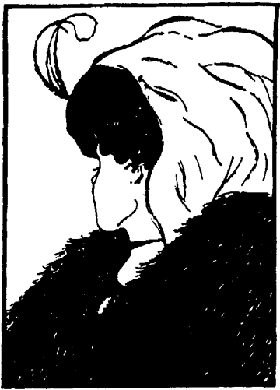
\includegraphics[width=1.58in,height=2.2in]{./image3.png}\hfill

\includegraphics[width=1.59in,height=2.2in]{./image4.png}\hfill

\includegraphics[width=1.9in,height=2.2in]{./image5.png}\hfill
\caption{Each of the images shown above has two different
interpretations. Can you determine what they are?}
\label{figure:differentInterpertations}
\end{figure}


One of the most common \emph{emotional blocks} is the fear of failure.
People often have creative ideas, but are afraid to express them since
they may be criticized or may not have the ``correct'' answer. It is
cliché to hear that you must fail often to succeed, but true. The highly
successful product design company, IDEO, that was examined in Chapter 2
takes the approach in con­cept generation to ``\emph{fail early and
often}'' in order to succeed {[}Kel01{]}. Their design teams are
en­couraged to develop many seemingly outlandish ideas that are often
discarded, but some­times lead to innovative solutions. Another emotional
block is a fear of chaos and disorgani­zation. The creative process
challenges engineers, since it is disorganized and not a neat scien­tific
approach to which they are accustomed. Another block is the tendency to
critically judge ideas, rather than generate and build upon them.
Finally, it takes time for creative ideas to incubate. Most of us can
relate to the experience when we could not solve a problem that nagged
us for a period of time, followed by that unexpected \emph{``Aha!''}
moment when we identi­fied the solution.

\emph{Environmental blocks} refer to those things in our environment
that limit creative ability. This could be in the form of poor teamwork
where members distrust each other and criticize each other's ideas. In
the workplace, this could be due to autocratic management that resists
new ideas. There are also cultural biases against creativity. There is a
bias against creativity as an approach to problem solving in the
engineering field. This is usually based upon the reasoning that there
is a single correct solution to a problem and creativity is an excuse
for poor engineering. It is true that creativity and brainstorming alone
do not solve engineering problems---the concepts generated need to be
scrutinized using engineering principles to become viable innovations.

The final block that Adams identified is that of \emph{intellectual and
expressive}. In an engi­neering context, this means that the designer
needs to have an understanding of intellectual tools that are applied to
solve problems. For example, mathematics is a universal language for
expressing and solving scientific problems. Specific examples in ECE are
languages that de­scribe the characteristics of systems such as
functional, logical, and state behaviors. Examples in digital design are
truth tables (input, output behavior) and state diagrams
(stimulus-response). In the domain of electronics design, a functional
approach (input, output, and function) is commonly used. Chapters 5 and
6 present tools for modeling the behavior of ECE systems.

\subsection{Vertical and Lateral Thinking}
\label{subsection:vertical-and-lateral-thinking}

Edward DeBono is the father of a field known as \emph{\textbf{lateral
thinking}}, which offers a different per­spective on the barriers to
creativity. Lateral thinking is contrasted to what is known as the
vertical thinking process {[}Deb67, Deb70{]}. Engineers tend to be
vertical (or convergent) think­ers, meaning that they are good at taking
a problem and proceeding logically to the solution. This is typically a
sequential linear process, where the engineer starts at the highest
level and successively refines elements of the design to solve the
problem. This is usually based upon experience solving similar problems
and conventional tools that are employed in that par­ticular area.

The objective of lateral (or divergent) thinking is to identify creative
solutions. It is not concerned with developing the solution for the
problem, or right or wrong solutions. It encourages jumping around
be­tween ideas. In the words of DeBono ``\emph{The vertical thinker says:
\textquotesingle I know what I am looking for.\textquotesingle{} The
lateral thinker says: \textquotesingle I am looking but I
won\textquotesingle t know what I am looking for until I have found
it.\textquotesingle{}} '' The field of lateral thinking is characterized
by puzzles of the following type found at Paul Sloane's Lateral Thinking
Puzzles website {[}\url{http://dspace.dial.pipex.com/sloane}{]}:

\begin{itquote}
A body is discovered in a park in Chicago in the middle of summer. It
has a fractured skull and many other broken bones, but the cause of
death was hypothermia.\\ \\

A hunter aimed his gun carefully and fired. Seconds later, he realized
his mistake. Minutes later, he was dead.\\ \\

A man is returning from Switzerland by train. If he had been in a
non-smoking car he would have died.
\end{itquote}

The objective in these puzzles is to develop plausible scenarios that
explain how each of the above situations could have happened. A solution
for the first example is that a person stowed away in the wheel
compartment of a jet airliner. While in flight he froze and died of
hypo­thermia. When the plane prepared to land, it lowered its landing
gear, causing the body to fall to the park, fracturing his skull, and
breaking his bones. Can you develop plausible scenarios that describe
each of them?

Vertical thinking focuses on sequential steps toward a solution and
tries to determine the correctness of the solution throughout the
process. This is very different from lateral thinking where there is
nonlinear jumping around between steps and there is no attempt to
discern be­tween right and wrong. As such, lateral thinking is more apt
to follow least likely paths to a solution, whereas vertical thinking
follows the most likely paths. The goal in lateral thinking is to
develop as many solutions as possible, while vertical thinking tries to
narrow to a single solution.

Lateral thinking is appropriate for the concept generation phase. So
should concept gen­eration and brainstorming be done by the individual or
by a team? DeBono and Osborn {[}Osb63{]} conclude that creativity is
more effective by individuals than by teams. However, Osborn also points
out that there is great value in applying creativity in teams, since it
provides a place for the team to work together on problems and see other
perspectives. Our anecdotal observations of student design teams
supports this---group brainstorming is effective for developing
concepts, new product ideas, new features, and different ways to combine
technologies. This is because in groups, ideas are readily built upon by
other team members. More mathe­matical, technical, and theoretical
breakthroughs tend to be the work of the lone genius. Ex­amples of this
are the Theory of Relativity (Einstein), Boolean Logic (Bool), and
Shannon's Sampling Theorem. We have also observed that novice designers,
who do not have much experience in concept generation, can benefit
greatly from group brainstorming techniques.

\subsection{Strategies to Enhance Creativity}
\label{subsection:strategies-to-enhance-creativity}

There are valuable strategies that can be employed to enhance the
creative process. The body of research on the subject is very large and
key points are summarized as follows:

\begin{itemize}
\item
  \emph{Have a questioning attitude.} One of the keys is to have a
  questioning attitude and chal­lenge assumptions. The willingness to do
  this generally decreases as people age. Young children are highly
  creative and are constantly questioning everything, with questions
  such as ``\emph{Why do trees have leaves?}'' or ``\emph{Why is the sky
  blue?}'' Asking basic questions stimulates creativity and is
  applicable to technical designs. When examin­ing a design with a
  microcontroller, ask questions such as ``\emph{Is there a way to
  replace the microcontroller?}''\emph{,} ``\emph{Are there other
  features that I can achieve with the microcontroller?}''\emph{,} and
  ``\emph{Is there a better microcontroller that can be used?}''
\item
  \emph{Practice being creative.} Research shows that people can improve
  their creative ability through conscious effort. For example, try
  solving the puzzles presented in this chapter and in the end of the
  chapter problems. Be conscious of things that bother you (``pet
  peeves'') in your everyday life and try to develop new solutions for
  them.
\item
  \emph{Suspend judgment.} It is easy to criticize and immediately
  dismiss ideas, so it is impor­tant to defer judgment and be flexible in
  thinking. Seemingly outlandish ideas can lead to other concepts that
  are valuable solutions. The opportunity for new solutions is curtailed
  if ideas are immediately judged and discarded. Creative concepts can
  be developed by taking a concept and modifying it or combining it with
  other seemingly unrelated concepts.
\item
  \emph{Allow time.} The creative process needs time for incubation. The
  human mind needs time to work on problems, so set aside time to
  reflect on the problem and to allow it to incubate so that the
  ``\emph{Aha!}'' moment of discovery can happen.
\item
  \emph{Think like a beginner.} New solutions often come from novices.
  The reason is that nov­ices don't have preconceived ideas as to the
  solution for a problem. Experience is a double-edged sword---it allows
  one to quickly solve problems by drawing upon pre-existing solutions,
  but can inhibit creativity. If confronted with a new problem that
  bears similarity to one encountered in the past, then it is likely
  that the new solution will bear similarity to the old one. If everyone
  else is it doing it one way, consider the opposite.
\end{itemize}

Many creative ideas arise from novel combinations and adaptations of
existing technology. SCAMPER, an acronym for Substitute, Combine, Adapt,
Modify, Put to other use, Eliminate, and Rearrange/Reverse, can be used
as a guide to systematically generate creative concepts. The SCAMPER
principles are valuable in brainstorming and are described below:

\begin{itemize}
\item
  \emph{Substitute.} Can new elements be substituted for those that
  already exist in the system?
\item
  \emph{Combine.} Can existing entities be combined in a novel way that
  has not been done be­fore?
\item
  \emph{Adapt.} Can parts of the whole be adapted to operate
  differently?
\item
  \emph{Modify.} Can part or all of a system be modified? For example,
  size, shape, or functional­ity.
\item
  \emph{Put to other use.} Are there other application domains where the
  product or system can be put to use?
\item
  \emph{Eliminate.} Can parts of the whole be eliminated? Or should the
  whole itself be elimi­nated?
\item
  \emph{Rearrange or Reverse.} Can elements of the system be rearranged
  differently to work bet­ter? This is different from substituting in
  that the elements of the system are not changed, but rearranged or
  ordered differently to create something new. In terms of reversal, are
  there any roles or objectives that can be reversed?
\end{itemize}

SCAMPER is a modification of a set of questions that was originally
posed by Osborn {[}Osb63{]} and was modified to its form above by
Michalko {[}Mic91{]}.

\section{Concept Generation}
\label{section:concept-generation}

After the problem is defined, the next step is to explore concepts for
the solution. It is unlikely that a design team will have reached this
stage without some ideas for solving the problem, but it is important to
fully explore the design space. Ullrich and Eppinger {[}Ull03{]}
identify the following phases of concept generation -- search
internally, search externally, and systematically explore. Each is
considered in turn.

External searching was covered to a great extent in Chapters 2 and 3,
which addressed conducting background research and benchmarking. Methods
of external searching are:

\begin{itemize}
\item
  Conduct literature search.
\item
  Search and review existing patents.
\item
  Benchmark similar products.
\item
  Interview experts.
\end{itemize}

Internal searching is done by the team members via methods such as
brainstorming. The team members need have to have a common problem
definition for this to be effective. Understanding the tradeoffs using
requirement analysis methods in Chapter 3 is also valuable, as
overcoming tradeoffs leads to innovative solutions. Furthermore, the
team should decompose larger problems into sub-problems and the attack
the sub-problems individually. Chapter 5 addresses the process of
problem decomposition.

\textbf{DILBERT\textsuperscript{®} by Scott Adams}
\begin{figure}

\includegraphics[width=5.49in,height=1.96in]{./image6.png}
\caption{Wally brainstorming. (Dilbert © United
Feature Syndicate. Reprinted by permission.}
\label{figure:dilbertConcept}
\end{figure}

The most well-known method of internal searching is
\emph{\textbf{brainstorming}}. Group brainstorming is effective for
generating many concepts in a short period of time. Experienced design
teams are known to generate hundreds of concepts in an hour. Traditional
brainstorming is not highly-structured---though a facilitator
helps---and employs five basic rules:

\begin{itemize}
\item
  No criticism or judgment of ideas.
\item
  Wild ideas are encouraged.
\item
  Quantity is stressed over quality.
\item
  Build upon and modify the ideas of others.
\item
  All ideas are recorded.
\end{itemize}

Many novice design teams struggle with unstructured brainstorming and
more formalized approaches, such as brainwriting and the Nominal Group
Technique, can be of benefit. The steps of \emph{\textbf{brainwriting}}
are:

\begin{enumerate}
\def\labelenumi{\arabic{enumi}.}
\item
  The team develops a common problem statement that is read out loud.
\item
  Each team member writes their ideas down on a card and places it in
  the center of the table.
\item
  Other team members then take cards from the pile and use other's ideas
  to generate new ones or build upon them, keeping in mind the
  principles of SCAMPER. Alternatively, members can each generate an
  idea, write it on a card, and then pass it to another team member.
  Each member then builds upon the idea passed to them.
\end{enumerate}

\emph{\textbf{Brainwriting 6-3-5}} is a variation where the objective is
to have six people, develop three ideas in five minutes. The optimal
number of people for the exercise is thought to be six, although it is
not necessary. Each person generates three ideas in five minutes, and
clearly describes it using sketches and written descriptions on paper.
At the end of five minutes, each team member passes their ideas to
another team member. The next person reviews the ideas of their teammate
and adds three more by building on them, developing new ones, or
ignoring as necessary. This process continues until all members have
reviewed all papers.

In the \emph{\textbf{Nominal Group Technique}} (NGT) {[}Del71{]} each
team member silently generates ideas that are reported out in a
round-robin fashion so that all members have an opportunity to present
their ideas. Concepts are selected by a multi-voting scheme with each
member casting a predetermined number of votes for the ideas presented.
The ideas are then ranked, discussed further, and voted upon again if
necessary. The steps of NGT are as follows:

\begin{itemize}
\item
  \emph{Read problem statement.} It should be read out loud by a team
  member (the facilitator).
\item
  \emph{Restate the problem.} Each person restates the problem in their
  own words to ensure that all members understand it.
\item
  \emph{Silently generate ideas}. All members silently generate ideas
  during a set period of time, typically 5--15 minutes.
\item
  \emph{Collect ideas in a round-robin fashion}. Each person presents
  one idea in turn until all ideas are exhausted. The facilitator should
  clarify ideas and all should be written where the entire team can view
  them.
\item
  \emph{Summarize and rephrase ideas.} Once the ideas are collected, the
  facilitator leads a discus­sion to clarify and rephrase the ideas. This
  ensures that the entire group is familiar with them. Related ideas can
  be grouped or merged together.
\item
  \emph{Vote.} Each person casts a predetermined number of votes,
  typically three to six, for the ideas presented. The outcome is a set
  of prioritized ideas that the team can further discuss and pursue.
\end{itemize}

To systematically generate concepts, the problem is decomposed
sub-functions and solutions are sought for the sub-functions. A
\emph{\textbf{concept table}}, demonstrated in 
Table~\ref{table:conceptPersonalComputing}, is a tool for
identifying different combinations, arrangements, and substitutions. The
table headings identify functions to be achieved in the design, while
the entries in the corresponding column represent po­tential solutions.
Novel products or solutions are generated by combining elements from
each of the columns, which are identified in the table by circled
elements. The solutions can be in the form of a single element selected
from each column, or as in the example shown, multiple elements selected
from each column.

\begin{table}
\caption{A concept table for generating ideas for a personal
computing system. The potential so­lution is identified by the
combination of circled elements.}
\label{table:conceptPersonalComputing}
\begin{tabular}{|p{2cm}|c|p{2cm}|c|p{2cm}|}
\hline
\rowcolor{Gray}
\textbf{User Interface}&
\textbf{Display} &
\textbf{Connectivity \& Expansion} &
\textbf{Power} &
\textbf{Size}\\ \hline
Keyboard & CRT & Serial \& Parallel & Battery & Hand-held, Fits in pocket \\ \hline
Touchpad & Flat Panel & USB & AC Power & Notebook size \\ \hline
Handwriting Recognition & Plasma & Wireless Ethernet & Solar Power & Wearable \\ \hline
Video & Heads-up Display & Wired Ethernet & Fuel Cell & Credit Card Size \\ \hline
Voice & LCD & PCMCIA & Thermal Transfer & Flexible in shape \\ \hline
& & Modem / Telephone & & \\ \hline
\end{tabular}
\end{table}

Based on the concepts circled in 
Table~\ref{table:conceptGeneration}, one can imagine a personal
computing system that has the following features: 1) is wearable with
different credit card size components placed on the body and in clothing
to make it comfortable to use; 2) is powered by a combina­tion of solar
cells, fuel-cells, and from thermal heat generated by a person's body;
3) has a mi­crophone and camera integrated in the user's clothing for
interface to the system, as well as a flexible foldable keyboard for
typing that is stored in a pocket; 4) has a heads-up display inte­grated
with the user's eyeglasses or baseball hat; and 5) has a miniature
earpiece microphone used for communication. While the above example
focused on novel combinations and substitu­tions, the concept table can
also be used to examine the possibility of eliminating ideas. For
example, the table inherently assumes that a display will be used.
However, it should also be asked if it is abso­lutely necessary in the
design.

Another example is shown in Table~\ref{table:conceptTemperature}, 
where the objective is to
identify design concepts for a temperature measurement and display
device. There are three main elements to the pro­posed solution: the
thermal sensing method, circuitry that converts the sensor in­formation
(temperature) to a voltage, and a display unit that converts the voltage
to a dis­played temperature. Note that the table implies a three-stage
architecture, thus concepts are generated within that framework. There
may be completely different architec­tures that are better.


\begin{table}
\caption{Concept table for a temperature measurement device.}
\label{table:conceptTemperature}
\begin{tabular}{|c|c|c|}
\hline
\rowcolor{Gray}
\textbf{Thermal Sensing} &
\textbf{Conversion to Voltage} &
\textbf{Display} \\ \hline
Thermistor & Op Amp Design & Seven-Segment LEDs \\ \hline
RTD & Transistor Designs & LCD \\ \hline
Thermocouple & & Analog Dial Indicator \\ \hline
\end{tabular}
\end{table}

A related tool is a \emph{\textbf{concept fan}}, which is a graphical
representation of design decisions and choices. An example concept fan
for the temperature measuring device is shown in 
Figure~\ref{figure:conceptFan}. Design
decisions are identified by circles; solutions are indicated by squares.
In this example, more options are shown than in 
Table~\ref{table:conceptTemperature}. Concepts are
generated by selecting among the different solution blocks.

\begin{figure}
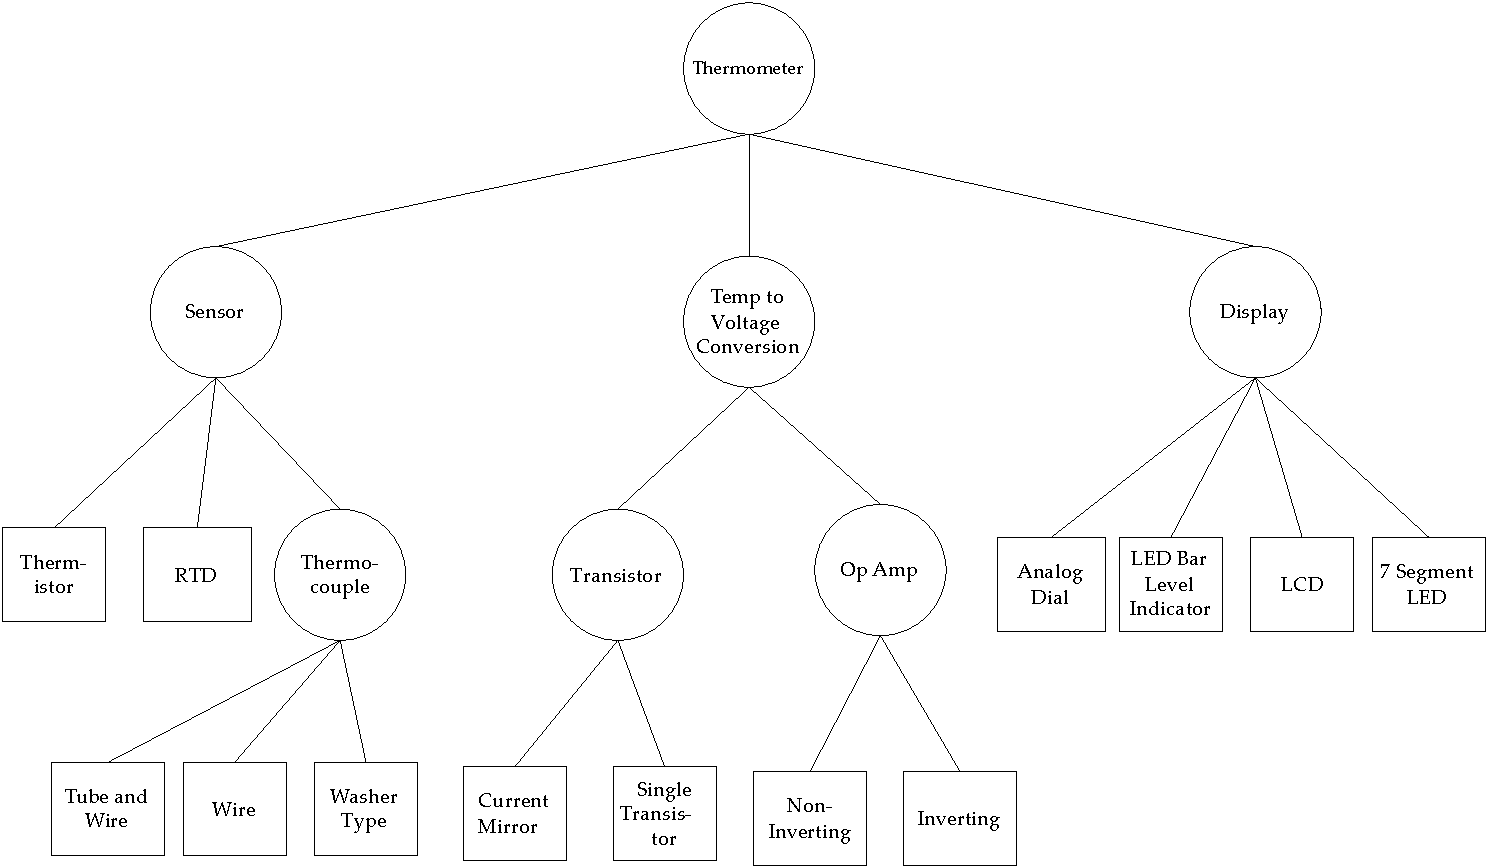
\includegraphics[width=5.5in,height=3.2in]{./image7}
\caption{A concept fan for the temperature measuring device.
The circles represent the choices to be made and the squares represent
potential solutions to the choices.}
\label{figure:conceptFan}
\end{figure}


\subsection{Concept Evaluation}\label{concept-evaluation}

The concepts generated are evaluated to determine which are the most
promising to pursue. The designer should exercise engineering judgment
and use the customer needs and technical factors to drive the decision.
This process is shown in 
Figure~\ref{figure:conceptFan}, where the user needs, concepts, and
engineering consideration serve as inputs to a decision process to ranks
the concepts. A point of caution---some of the methods presented
generate numerical scores for comparing concepts, leading one to
potentially believe that the quantita­tive results are infallible. Keep
in mind that the inputs are based on qualitative and semi-quantitative
assessments and can be geared to select a preconceived notion of the
solution. It is important to maintain flexibility of thinking, to
challenge assumptions, and ultimately determine the best concept.

\begin{figure}
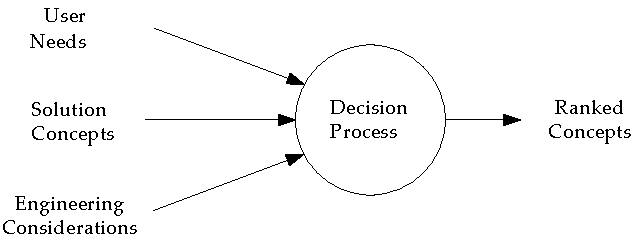
\includegraphics[width=3.35in,height=1.1in]{./image8}
\caption{Process for concept evaluation.}
\label{figure:conceptFan}
\end{figure}


\subsection{Initial Evaluation}
\label{subsection:initial-evaluation}

The concepts generated should be initially reviewed and those that are
completely infeasible discarded. Some of the reasons a concept may be
deemed infeasible are that it may be far too costly, will take too long
to develop, or involve too much risk. In many cases it may be deemed
that using cutting-edge technology represents an unacceptable risk.
Concepts that clearly cannot meet the engineering requirements should
also be discarded. Care should be taken not to completely eliminate
ideas that may have merit, as conditions change and some concepts that
were previously thought unrealistic may become viable in the future.

\subsection{Strengths and Weaknesses Analysis}
\label{subsection:strengths-and-weaknesses-analysis}

Another form of evaluation is to complete a \emph{\textbf{strengths and
weaknesses analysis}} of the potential solutions. 
Table~\ref{table:strengthWeakIntel} demonstrates
the application of this analysis applied to an experi­mental design
project for testing of the Intel 1000XF card (examined in Chapter 2
(Example 2.2) and Chapter 3 (Table 3.2)). In order to test the card
under different operating temperatures, a method of heating the card and
holding its temperature fixed during the experiment was needed. The two
solutions compared were to use a contact heating element or to place the
card in an environmental test chamber. In this particular example, the
temperature chamber solution was ultimately selected due to the need for
a uniform temperature distribution. The strength and weakness analysis
is good for examining problems of moderate complexity. It suffers in
that it does not require uniform criteria for comparison. To make the
method more quantitative, relative scores for the strengths (plus
factors) and weaknesses (minus factors) can be assigned and used to
score the concepts.

\begin{table}

\caption{A strengths and weaknesses analysis of proposed
methods for heating an Intel 1000XF card to be used in lifetime testing.
{[}Ese03{]}.}
\label{table:strengthWeakIntel}
\begin{tabular}{|m{3cm}|m{5cm}|m{5cm}|}
\hline
\textbf{Method} &
\textbf{Strengths} &
\textbf{Weaknesses} \\ \hline

\textbf{Contact Heating} & 
\begin{itemize}
\item   Simplest design
\item   Could be used internally to computer
\end{itemize}   &

\begin{itemize}
\item   Does not create uniform tem­perature
\item   Hard to control tempera­ture
\end{itemize} \\ \hline

\textbf{Temperature Chamber} &
\begin{itemize}
\item  Uniform tempera­ture
\item  Greater control over tem­perature
\end{itemize}
&
\begin{itemize}
\item   Must be external to computer
\item   More difficult to design
\item   Expensive
\end{itemize}\\ \hline

\end{tabular}
\end{table}

\subsection{Analytical Hierarchy Process and Decision Matrices}
\label{subsection:analytical-hierarchy-process-and-decision-matrices}

In the Analytical Hierarchy Process, design alternatives are compared
against pre-selected criteria, such as the engineering or marketing
requirements. AHP is covered in detail in Appendix B and was first
applied in Chapter 2 for project selection. The reader is encouraged to
review Appendix B as necessary. The end result of AHP is a decision
matrix is shown in 
Table~\ref{table:decisionMatrixAHP}, where the criteria are listed in the
leftmost column with the associated weighting factors
($\omega_i$) quantifying the relative
importance of the criteria. The body of the matrix contains design
ratings, $\alpha_{ij}$, that reflect the
technical merit of each of the \emph{j\textsuperscript{th}} design
options relative to \emph{i\textsuperscript{th}} criterion. The total
score, \emph{S\textsubscript{j}}, for each design option is computed as
a weighted summation of the design ratings and weighting factors.

\begin{table}
\caption{A decision matrix for the Analytical Hierarchy Process.}
\label{table:decisionMatrixAHP}

\begin{tabular}{|c|c|c|c|c|c|}
\hline
\rowcolor{Gray}
\multicolumn{2}{c}{}  & 
\textbf{Design Option 1} & 
\textbf{Design Option 2} & 
                                         &
\textbf{Design Option n} \\ \hline

\textbf{Criteria 1}  	&
$\omega_1$ 			&
$\alpha_{11}$			&
$\alpha_{12}$			&
$\dots$				&
$\alpha_{1n}$		 \\ \hline


\textbf{Criteria 2} 		& 
$\omega_2$ 			&
$\alpha_{21}$			&
$\alpha_{22}$			&
$\dots$				&
$\alpha_{2n}$		 \\ \hline

\textbf{Criteria \emph{m}} & 
$\omega_m$ 		&
$\alpha_{m1}$		&
$\alpha_{m2}$		&
$\dots$				&
$\alpha_{mn}$		 \\ \hline


\multicolumn{2}{|c|} {\textbf{Score}}  & 
$S_1 =  \sum_{i=1}^{m} \omega_i * \alpha_{i1}$    &
$S_2 = \sum_{i=1}^{m} \omega_i * \alpha_{i2} $   &
$\dots$							&
$S_n = \sum_{i=1}^{m} \omega_i * \alpha_{im} $   \\ \hline

\end{tabular}
\end{table}

The application of AHP is demonstrated for the design of an electronic
circuit for measuring temperature, by producing a voltage signal that is
directly proportional to temperature.

\subsection*{Step 1: Determine the Selection Criteria}
\label{subsection:step-1-determine-the-selection-criteria}

Assume that the criteria for comparing the concepts are high accuracy,
low cost, small size, and availability of parts for manufacture.

\subsection*{Step 2: Determine the Criteria Weightings}
\label{subsection:step-2-determine-the-criteria-weightings}

  Assume that the criteria were ranked using pairwise comparison and
  weights computed (see Appendix B) as shown in 
  Table~\ref{table:pairwiseCompMatrix}.

\begin{table}
\caption{Pairwise comparison matrix.}
\label{table:pairwiseCompMatrix}

\begin{tabular}{|c|c|c|c|c|c|}
\hline
  &
\textbf{Accuracy}&
\textbf{Cost}&
\textbf{Size}&
\textbf{Availability}& 
\textbf{Weights} \\ \hline

\textbf{Accuracy} & 1 & 5 & 3 & ¼ & 0.42 \\ \hline
\textbf{Cost} & 1/5 & 1 &  2  & ¼ & 0.12 \\ \hline
\textbf{Size} & 1/3 & ½ & 1 & 1 & 0.12 \\ \hline
\textbf{Availability} & 4 & 4 & 1  & 1 & 0.34 \\ \hline
\end{tabular}
\end{table}

\subsection*{Step 3: Identify and Rate Alternatives Relative to the Criteria}
\label{subsection:step-3-identify-and-rate-alternatives-relative-to-the-criteria}

Three candidate solutions are shown in 
Figure~\ref{figure:solutionsTemperature}. Each acts as a
constant current source that drives a temperature measurement device
(RTD). The resistance of an RTD varies with temperature, and when driven
by a constant cur­rent, \emph{I}, produces a voltage,
\emph{V\textsubscript{T}}, that varies proportionally with temperature.
Each circuit supplies a constant current of I=1mA.

\begin{figure}
\caption{Candidate solutions for temperature measurement.}
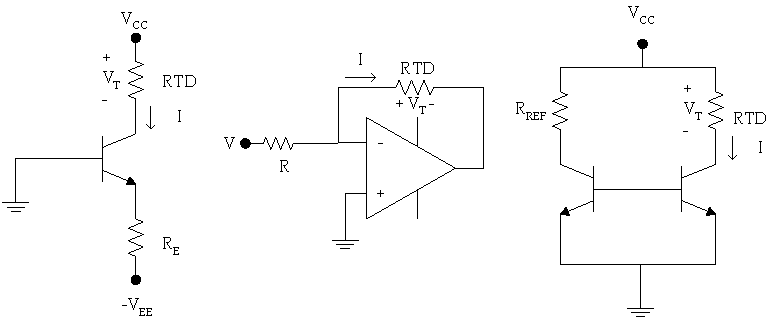
\includegraphics[width=5.5in,height=2.3in]{./image20}
1: Single Transistor 2: Inverting Op Amp 3: Current Mirror
\label{figure:solutionsTemperature}
\end{figure}

The accuracy of each design was evaluated by a sensitivity analysis
using a SPICE cir­cuit simulation package assuming 10\% resistors. The
deviation of the output volt­age (maximum deviation from nominal) for the
three designs is 9.2\%, 1.3\%, and 1.9\% respectively. Since the
objective is to minimize the deviation, the following rating metric is
used:
$$ \alpha = \frac{min[deviation]}{deviation}$$
This produces the following normalize design ratings for accuracy:
$\alpha{11} = 0.008$, 
$\alpha{12} = 0.55$, and 
$\alpha{13} = 0.37$.

The parts costs are the following: resistors = \$0.05, bipolar junction
transistors (BJTs) = \$0.15, op amps = \$0.35, and RTDs = \$0.25. Using
a measure for cost similar to (1) gives following normalized cost
ratings for the three options
respec­tively:
$\alpha{21} = 0.31$, 
$\alpha{22} = 0.28$, and 
$\alpha{23} = 0.31$.

Assume that to manufacture each circuit on a printed circuit board
requires the following dimen­sions: design 1 = 1 in\textsuperscript{2},
design 2 = 1.56 in\textsuperscript{2}, and design 3 = 2.25
in\textsuperscript{2}. The objective is to minimize size, and againusing
a measure analogous to (1) for the required space to manufacture each
produces the following normalized decision ratings:
$\alpha{31} = 0.48$, 
$\alpha{32} = 0.31$, and 
$\alpha{33} = 0.21$.

Assume that the parts have an in-stock availability of 95\%, 70\%, 90\%,
and 80\% of the time for the resistors, BJTs, RTDs, and op amps
respectively. A measure for the overall availability of parts to
manufacture each design is re­quired. One way to measure this is to
compute the probability that a design will be able to be manufactured
based upon the past history of part availability. This is found by
multiplying the availability of all individual components needed for the
design:

\emph{P}(design 1 can be produced) \emph{=} (0.95)(0.90)(0.70) = 0.60

\emph{P}(design 2 can be produced) \emph{=} (0.95)(0.90)(0.80) = 0.68

\emph{P}(design 3 can be produced) \emph{=} (0.95)(0.90) (0.70)(0.70) = 0.42

This produces the following normalized decision ratings for availability:
$\alpha{41} = 0.35$, 
$\alpha{42} = 0.40$, and 
$\alpha{43} = 0.25$.

\subsection*{Step 4: Compute Scores for the Alternatives}
\label{subsection:step-4-compute-scores-for-the-alternatives}

The decision matrix is built and the overall weighted scores for the
alternatives are computed as shown in Table~\ref{table:decisionMatrix}.

\begin{table}
\caption{The decision matrix.}
\label{table:decisionMatrix}
\begin{tabular}{|c|c|c|c|c|}
\hline
\multicolumn{2}{|c|}{}  & 
\textbf{Single BJT} & 
\textbf{Op Amp} &
\textbf{Current Mirror} \\ \hline
\textbf{Accuracy} & 0.42 & 0.08 & 0.55 & 0.37 \\ \hline
\textbf{Cost} & 0.12 & 0.41 & 0.28 & 0.31 \\ \hline
\textbf{Size} & 0.12 & 0.48 & 0.31 & 0.21 \\ \hline
\textbf{Availability} & 0.34 & 0.35 & 0.40 & 0.25 \\ \hline
\multicolumn{2}{|c|} {\emph{\textbf{Score}}} & 0.26 & 0.44 & 0.30 \\ \hline
\end{tabular}
\end{table}

\subsection*{Step 5: Review the Decision}
\label{subsection:step-5-review-the-decision}


Remember that this is a semi-quantitative method. The final ranking
indicates that design options 1 and 3 are quite similar, while both are
inferior to option 2.

\subsection{Pugh Concept Selection}
\label{subsection:pugh-concept-selection}

Pugh Concept Selection is a method of comparing concepts against
criteria, similar to what we saw with a decision matrix. It is different
in that it has a simpler scoring method and it is an iterative process.
The steps of Pugh Concept Selection are:

\begin{enumerate}
\def\labelenumi{\arabic{enumi}.}
\item
  Select the comparison criteria, usually the engineering or marketing
  requirements.
\item
  Determine weights for the criterion.
\item
  Determine the concepts.
\item
  Select a baseline concept that is initially believed to be the best.
\item
  Compare all other concepts to the baseline, using the following
  scoring method: +1 better than, 0 equal to, -1 worse than.
\item
  Compute a weighted score for each concept, not including the baseline.
\item
  Examine each concept to determine if it should be retained, updated,
  or dropped. Synthesize the best elements of others into other concepts
  wherever possible.
\item
  Update the table and iterate until a superior concept emerges.
\end{enumerate}

An example of a Pugh Concept Selection matrix is shown in 
Table~\ref{table:pughConceptSelection}.

\begin{table}
\caption{Pugh Concept Selection matrix.}
\label{table:pughConceptSelection}

\begin{tabular}{|c|c|c|c|c|c|}
\hline
\rowcolor{Gray}
\multicolumn{2}{c}{}    &
\textbf{Option 1  (Reference)}  &
\textbf{Option 2} &
\textbf{Option 3} &
\textbf{Option 4} \\ \hline
\textbf{Criteria 1} & 4 & - & 0 & 0 & +1 \\ \hline
\textbf{Criteria 2} & 5 & - & +1 & -1 & 0 \\ \hline
\textbf{Criteria 3} & 2 & - & -1 & 0 & +1 \\ \hline
\textbf{Criteria 4} & 1 & - & +1 & +1 & -1 \\ \hline
\multicolumn{2}{|c|} {\textbf{Score}} & - & 4 & -4 & 5 \\ \hline
\multicolumn{2}{|c|} {\textbf{Continue?}} & Combine & Yes & No & Combine \\ \hline
\end{tabular}
\end{table}

\section{Project Application: Concept Generation and Evaluation}
\label{section:project-application-concept-generation-and-evaluation}

The following advice is provided for teams in the concept generation and
evaluation phase:

\begin{itemize}
\item
  Set aside time specifically for concept generation and evaluation and
  take it as a challenge to identify as many concepts as possible.
\item
  Search externally, including literature reviews and patent searches.
\item
  Search internally using brainstorming, brainwriting, or the Nominal
  Group Technique. Effective teams generate many concepts in a
  brainstorming session.
\item
  Examine solutions for the entire design, for sub-functions of the
  design, and for individual components (such as integrated circuit
  selection). The tech­niques in this chapter can be combined with design
  methods presented in Chapters 5 and 6.
\item
  Utilize SCAMPER, concept tables, and concepts fans as tools to
  facilitate and document concept generation.
\item
  Critically and objectively evaluate concepts against common criteria.
\item
  Clearly identify the concept(s) selected and the rationale for
  selection.
\end{itemize}

\section{Summary and Further Reading}
\label{section:summary-and-further-reading}

In the design process, it is important to creatively generate different
concepts for a solution to a problem. This is followed by an evaluation
of concepts to determine which are the most promising. This chapter
identified barriers to creativity and provided strategies for enhancing
creative ability. The concepts of vertical and lateral thinking were
introduced, and their im­pact on the design process was explored. Methods
of concept generation, including brainstorming, concept tables, and
concepts fans were presented. Finally, methods for critically evaluating
concepts (strength/weakness analysis, Analytical Hierarchy Process, and
Pugh Concept selection) were presented.

There are many references that examine creativity and concept
generation. Adams {[}Ada01{]} is a good reference for creativity and
problem-solving with a technical bent. Alex Os­born was an advocate of
creativity and developed two readable works that address the creative
process, the need for creativity, and strategies for enhancing it
{[}Osb48, Osb63{]}. Ed­ward DeBono is another well-known authority in the
field and has produced many works on lateral thinking and creativity
{[}Deb67, Deb70{]}. Paul Sloane has published numerous books with
lateral thinking puzzles {[}Slo91, Slo93, Slo94{]}. TRIZ {[}Alt99{]} is
a more advanced and complex approach to concept generation, that centers
around resolving tradeoffs in a problem. It is fairly complex and may be
considered by more advanced teams.

%\section{Problems}
\label{section:problems}

\begin{enumerate}
\def\labelenumi{\arabic{enumi}.}
\item
  Consider the nine dot puzzle shown in Figure 4.1 (b). Draw
  \textbf{three} connected straight lines that pass through all nine
  dots.

\item
  Consider the six sticks shown below. Rearrange the sticks to produce
  four equilat­eral triangles (the sticks cannot be broken).
\item
  Consider the fish shown below made of eight sticks and a coin for the
  eye. The objective is to make the fish face the other direction by
  moving only the coin and three sticks.

\begin{figure}

\includegraphics[width=2in,height=1.35in]{image34.pdf}
\label{figure:dotsProblems}
\end{figure}

\item
  For each of the following lateral thinking puzzles, develop a
  plausible solution (from Paul Sloane's \ul{Lateral Thinking Puzzles}
  {[}http://dspace.dial.pipex.com/sloane{]}):

\begin{itemize}
\item
  A man walks into a bar and asks the barman for a glass of water. The
  barman pulls out a gun and points it at the man. The man says
  \textquotesingle Thank you\textquotesingle{} and walks out.
\item
  A woman had two sons who were born on the same hour of the same day of
  the same year. But they were not twins. How could this be so?
\item
  Why is it better to have round manhole covers than square ones?
\item
  A man went to a party and drank some of the punch. He then left early.
  Everyone else at the party who drank the punch subsequently died of
  poisoning. Why did the man not die?
\end{itemize}

\item
  Legislation was passed to allow handguns in the cockpits of passenger
  airliners to prevent hijacking. Brainstorm to develop concepts that
  prevent anyone other than the pilot from using the handgun.
\item
  Imagine if scientists and engineers were able to develop a technology
  that would allow people to be transported from any place on earth to
  another instantaneously. Brainstorm to determine the potential impact
  this would have on society.
\item
  Student advising at many colleges and universities is seen as an area
  that can be im­proved. Brainstorm to develop ideas as to how student
  advising could be improved at your college or university.
\item
  In your own words, describe what a concept table and a concept fan
  are.
\item
  Consider the problem solved in Section 4.3.2. For this example assume
  that:
\begin{itemize}

\item
  The following is the result of the paired comparison.

\begin{table}
\begin{tabular}{|c|c|c|c|c|}
\hline
              &
Accuracy &
Cost &
Size &
Availability \\ \hline
Accuracy & 1 & 1/3 & 2 & ½ \\ \hline
Cost & 3 & 1 & 5 & 1 \\ \hline
Size & 1/2 & 1/5 & 1 & 2 \\ \hline
Availability & 2 & 1 & ½ & 1 \\ \hline
\end{tabular}
\end{table}


\item
  The parts costs are the following: resistors = \$0.05, bipolar
  transistors (BJTs) = \$0.10, op amps = \$0.35, and RTDs = \$0.25.
\item
  The parts have an in-stock availability of 99\%, 90\%, 85\%, and 70\%
  of the time for the re­sistors, BJTs, RTDs, and op amps respectively.
\item
  Everything else is the same as presented in Section 4.3.2.
\end{itemize}

Compute the rankings of the design options using a weighted decision
matrix of the type shown in Table 4.5.


\item
  \textbf{Project Application.} Utilize the methods in this chapter to
  generate con­cepts for your particular design problem. Critically
  evaluate the concepts generated using one or more of the techniques
  presented in the chapter that is appropriate for the problem. Section
  4.4 pro­vides guidance on how to conduct this process and document the
  results.
\end{enumerate}



%\addcontentsline{toc}{chapter}{Part II - Design Tools}
%\chapter*{Part II - Design Tools}

%\section{System Design I: Functional
Decomposition}\label{system-design-i-functional-decomposition}

At Sony, we assume all products of our competitors will have basically
the same technology, price, performance, and features. Design is the one
thing that differentiates one product from another in the
marketplace.---Norio Ohgo, Chairman and CEO, Sony

After the technical concept is selected, it is translated into a
solution that satisfies the system require­ments. The designer must put
on paper, or the computer screen, a representation that is meaning­ful
and clear; in other words, a useful abstraction of the system.
Engineering designs are often com­plex, consisting of many systems and
subsystems, thus this representation should facilitate the design
process and effectively describe the system. In addition, it serves an
im­portant function in communicat­ing the design to all members of the
team. Imag­ine a scenario where each team member is responsible for
designing part of a large system. Each person de­velops their part in
isolation and several months later the team gets back together to
integrate the pieces. Of course, the system won't work unless the team
has collectively defined and communicated the functionality and
interfaces for all subsystems in the design.

This chapter presents a well-known design technique---known as
\emph{\textbf{functional decomposi­tion}}---that is intuitive, flexible,
and straightforward to apply. It is probably the most pervasive design
technique used for engineering systems and is applicable to a wide
variety of prob­lems that extend well be­yond electrical and computer
engineering. In functional decomposition, systems are designed by
de­termining the overall functionality and then iteratively decomposing
it into component subsys­tems, each with its own functionality.

The objective of this chapter is to present both basic design concepts
and the functional decomposition design technique. A process for
functional decomposition is provided and it is applied to examples in
analog electronics, digital electronics, and software systems.

Learning Objectives

By the end of this chapter, the reader should:

\begin{itemize}
\item
  Understand the differences between bottom-up and top-down design.
\item
  Know what functional decomposition is and how to apply it.
\item
  Be able to apply functional decomposition to different problem
  domains.
\item
  Understand the concepts of coupling and cohesion, and how they impact
  designs.
\end{itemize}

\subsection{Bottom-Up and Top-Down
Design}\label{bottom-up-and-top-down-design}

Two general approaches to synthesizing engineering designs are known as
\emph{\textbf{bottom-up}} and \emph{\textbf{top-down}}. In the case of
bottom-up, the designer starts with basic components and synthe­sizes
them to create the overall system. To use an analogy, consider the case
of creating an automobile. In the bottom-up approach, you have pieces of
the automobile, such as the tires, motor, axle, transmission,
alternator, and they are brought together to create a car. The
impli­cation is that the final system depends upon the parts at hand. In
other words, in the bottom-up approach, the parts and subsystems are
given, and from them an artifact is created.

The top-down approach is analogous to the concept of divide-and-conquer.
In top-down the designer has an overall vision of what the final system
must do, and the problem is parti­tioned into components, or subsystems
that work together to achieve the overall goal. Then each subsystem is
successively refined and partitioned as necessary. In the case of the
auto­mobile, the overall objective is determined; the major subsystems
are defined, such as electri­cal, power drive-train, and the suspension;
and then each subsystem is further refined into its component parts
until the complete system is designed.

A debate that continues in the design community revolves around which is
the better ap­proach. It might appear that top-down is better, since it
starts with the over­all goal (requirements) and from that a solution is
developed. Top-down is particularly valu­able on large projects with many
subsystems, where it is unlikely that bringing together pieces in an
ad-hoc fashion will successfully solve the problem. A disadvantage of
top-down design is that it tends to limit the solution space and
innovation. Top-down design is inclined to follow a vertical thought
process (Chapter 4) where the designer starts with a problem and
succes­sively refines the subsystems until a blueprint for solving the
problem is defined. Further­more, the designer cannot create a top-down
design in a vacuum without bottom-up knowl­edge of existing technology
and how the system can be realized.

Bottom-up has the advantage of lending itself to creativity. It allows
the designer to take different technologies and from them create
something new, allowing more ``\emph{what if?}'' questions to be asked.
Bottom-up design is applicable when there are constraints on the
components that can be used. This is a realistic scenario. Consider the
case of variant design, where the goal is to improve the performance of
an existing, or legacy, system. For example, automobile manufacturers
might have to redesign their models to meet new emissions, mileage, or
safety standards. If you are not starting with a new design and must
utilize existing systems, it requires bottom-up thinking. In reality,
most problems require a combination of bottom-up and top-down thinking,
and the designer must al­ternate between them.

In summary, it is most effective to work between bottom-up and top-down.
A completely top-down approach is not feasible because the designer must
have an understanding of the bottom level technology for the components
of the design hierarchy to be realistic. Likewise, com­pletely bottom-up
by itself is generally not feasible, particularly as the system
complexity grows.

\subsection{Functional Decomposition}\label{functional-decomposition}

Functional decomposition is a recursive process that iteratively
describes the functionality of all system components. It is analogous to
the mathematical concept of a function, for example, \emph{y=f(x)}. In
this function there is an input, \emph{x}, an output, \emph{y}, and a
transformation between the input and output, \emph{f()}. This is easily
extended to the case of multiple inputs and outputs where the inputs and
outputs are vectors, 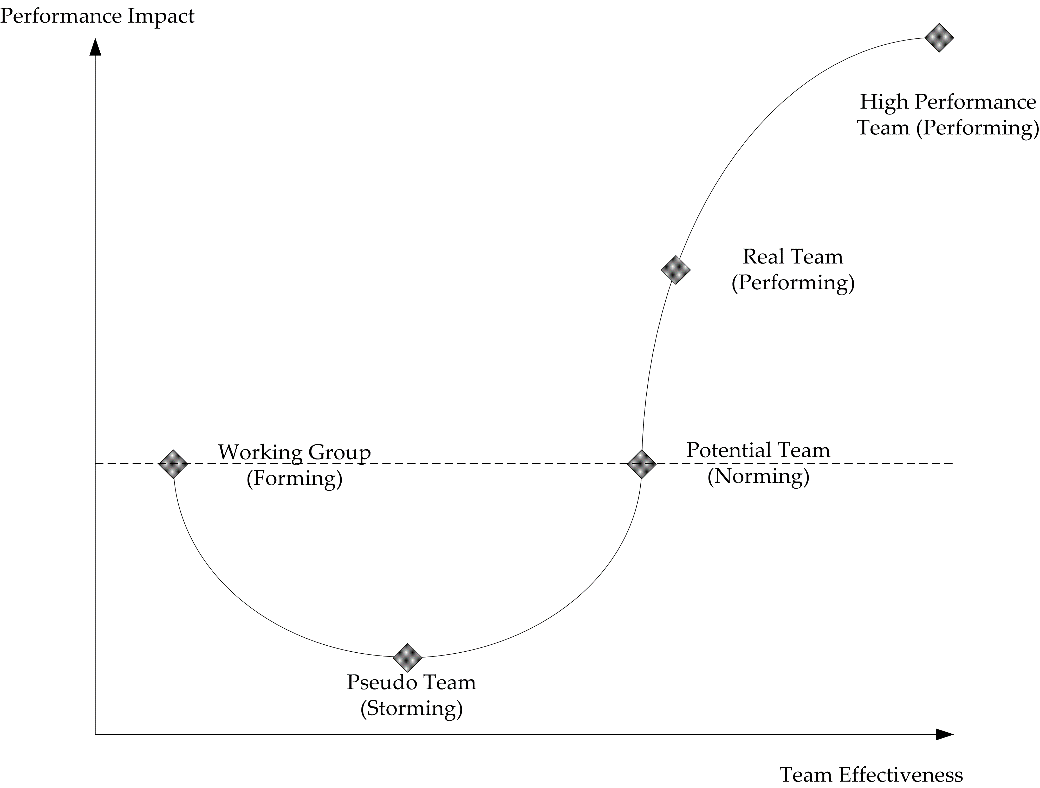
\includegraphics{media/image1.wmf}. In functional
decomposition, the same items are defined as in the mathematical
analogy---the inputs, the outputs, and the transformation between the
inputs and outputs (the functionality). Those three items constitute
what is known as the \emph{\textbf{functional specification}} or
\emph{\textbf{functional requirement}­---}the requirement that a
functional module should meet. A \emph{\textbf{module}} is a block, or
subsystem, that performs a function. Functional decomposition has a
strong top-down flavor, due to the fact that the highest level
functionality is defined and then further refined into sub-functions,
each with its own inputs, outputs, and functionality. The process is
repeated until some base level functionality is reached where the
modules can be actualized with physical components.

A process for applying functional decomposition is illustrated in Figure
5.1. It starts with a definition of the highest level (Level 0) of
system functionality (the functional requirement for the system). This
is followed by definition of the next level of the hierarchy that is
needed to achieve the design objective. The Level 1 design is typically
referred to as the main \emph{\textbf{design architecture}} of the
system. In this context, architecture means the organization and
interconnections between modules. Care must be taken at each design
level to ensure that it satisfies the requirements of the higher level.
The process is repeated for successive levels of the design and stops
when the \emph{\textbf{detailed design}} level is reached. Detailed
design is where the problem can be decomposed no further and the
identification of elements such as circuit components, logic gates, or
software code takes place. The number of levels in the design hierarchy
depends upon the complexity of the problem.

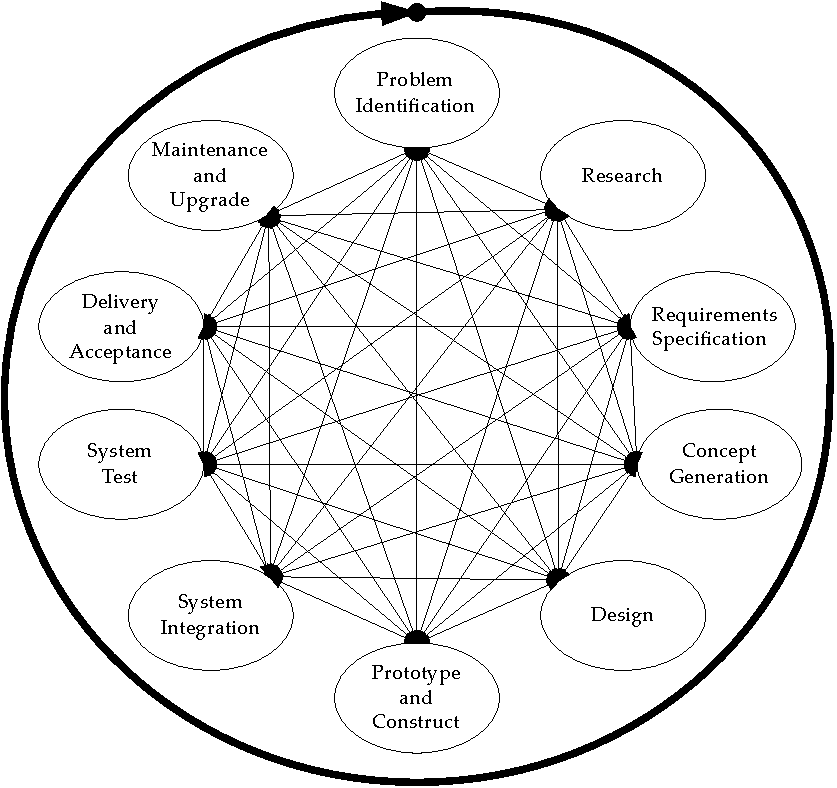
\includegraphics[width=5.47917in,height=1.69792in]{media/image2.emf}

\textbf{Figure 5.1} A process for developing designs using functional
decomposition.

\subsection{Guidance}\label{guidance}

The following guidance is provided before examining applications of the
functional decomposition technique:

\begin{itemize}
\item
  \emph{It is an iterative process}. During the first pass, it is not
  possible to know all of the detailed interfaces between components and
  the exact functionality of each block. In fact, some details are not
  known until the implementation level is reached, so the designer needs
  to iterate, work between top-down and bottom-up, and adjust the design
  as necessary.
\item
  \emph{Set aside sufficient time to develop the design}. This is a
  corollary to the previous point. The iterative nature means that it
  takes time to examine different solutions and to refine the details
  into a working solution.
\item
  \emph{Pair together items of similar complexity.} Modules at each
  level should have similar complexity and granularity.
\item
  \emph{A good design will have the interfaces and functionality of
  modules well-defined.} It is fairly easy to piece together some blocks
  into an apparently reasonable design. However, the functional
  requirements should be clearly defined and the technical feasibility
  understood. If not, the design will fall apart when it comes to the
  implementation stage. Consider the following advice of a well-known
  architectural designer:
\end{itemize}

\begin{quote}
The details are not the details. They make the design.---Charles Eames
\end{quote}

\begin{itemize}
\item
  \emph{Look for innovations.} Top-down designs tend to follow a
  vertical thinking process, where the designer proceeds linearly from
  problem to solution. Try to incorporate lateral thinking strategies
  from Chapter 4 and examine alternative architectures and technologies
  for the solution.
\item
  \emph{Don't take functional requirements to the absurd level.} Common
  elements, such as analog multipliers or digital logic gates, do not
  require explicit functional specifications. Doing so may become
  cumbersome and add little to the design. However, it depends upon the
  level at which you are working. If the goal is to design an analog
  multiplier chip, it is entirely appropriate to develop the functional
  requirement for the multiplier.
\item
  \emph{Combine functional decomposition with other methods of
  describing system behavior.} There is no single method or unifying
  theory for developing designs. Functional decomposition alone cannot
  describe all system behaviors. It may be supplemented by other tools
  such as flowcharts (logical behavior), state diagrams
  (stimulus-response), or data flow diagrams. In the digital stopwatch
  example presented later in this chapter, the behavior is defined using
  state diagrams. Other methods for describing system behavior are
  addressed in Chapter 6.
\item
  \emph{Find similar design architectures.} Determine if there exist
  similar designs and how they operate. Realize that this creates a bias
  towards existing solutions.
\item
  \emph{Use existing technology}. Many designers take the attitude that
  they are going to develop the entire design themselves, the sentiment
  being to ignore technology that they did not develop. Furthermore,
  engineering education predisposes us to design at a fundamental level.
  Both factors lead to time spent re-inventing the wheel. If existing
  technology is available that meets both the engineering and cost
  requirements, then use it.
\item
  \emph{Keep it simple}. Do not add complexity that is not needed.
\end{itemize}

\begin{quote}
\begin{quote}
A designer knows that he has achieved perfection not when there is
nothing left to add, but when there is nothing left to take
away.---Antoine de St-Exupery
\end{quote}
\end{quote}

\begin{itemize}
\item
  \emph{Communicate the results}. It is important to describe the theory
  of operation (the \emph{why}) as well as the implementation (the
  \emph{what}). The \emph{what} in the completed design is usually quite
  clear from the implementation, but documenting the description of
  operation and design decisions helps later when the system must
  upgraded. Designs can also become very complex, so consider how much
  information can be effectively communicated on a single page. If the
  information is too complex to show reasonably on a page or two, then
  it probably is too detailed and another level in the hierarchy should
  be added.
\end{itemize}

\subsection{Application: Electronics
Design}\label{application-electronics-design}

We now examine the application of functional decomposition in different
problem domains. In the domain of analog electronics, the inputs and
outputs of modules are voltage and current signals. Typical
transformations applied to the inputs are alterations in amplitude,
power, phase, frequency, and spectral characteristics. Consider the
design of an audio power amplifier that has the following engineering
requirements.

The system must

\begin{itemize}
\item
  Accept an audio input signal source with a maximum input voltage of
  0.5V peak.
\item
  Have adjustable volume control between zero and the maximum volume
  level.
\item
  Deliver a maximum of 50W to an 8Ω speaker.
\item
  Be powered by a standard 120V 60Hz AC outlet.
\end{itemize}

\subsubsection*{Level 0}\label{level-0}
\addcontentsline{toc}{subsubsection}{Level 0}

The Level 0 functionality for the amplifier is shown in Figure 5.2,
which is fairly simple---the inputs are an audio signal, volume control,
and wall outlet power, and the output is an amplified audio signal.

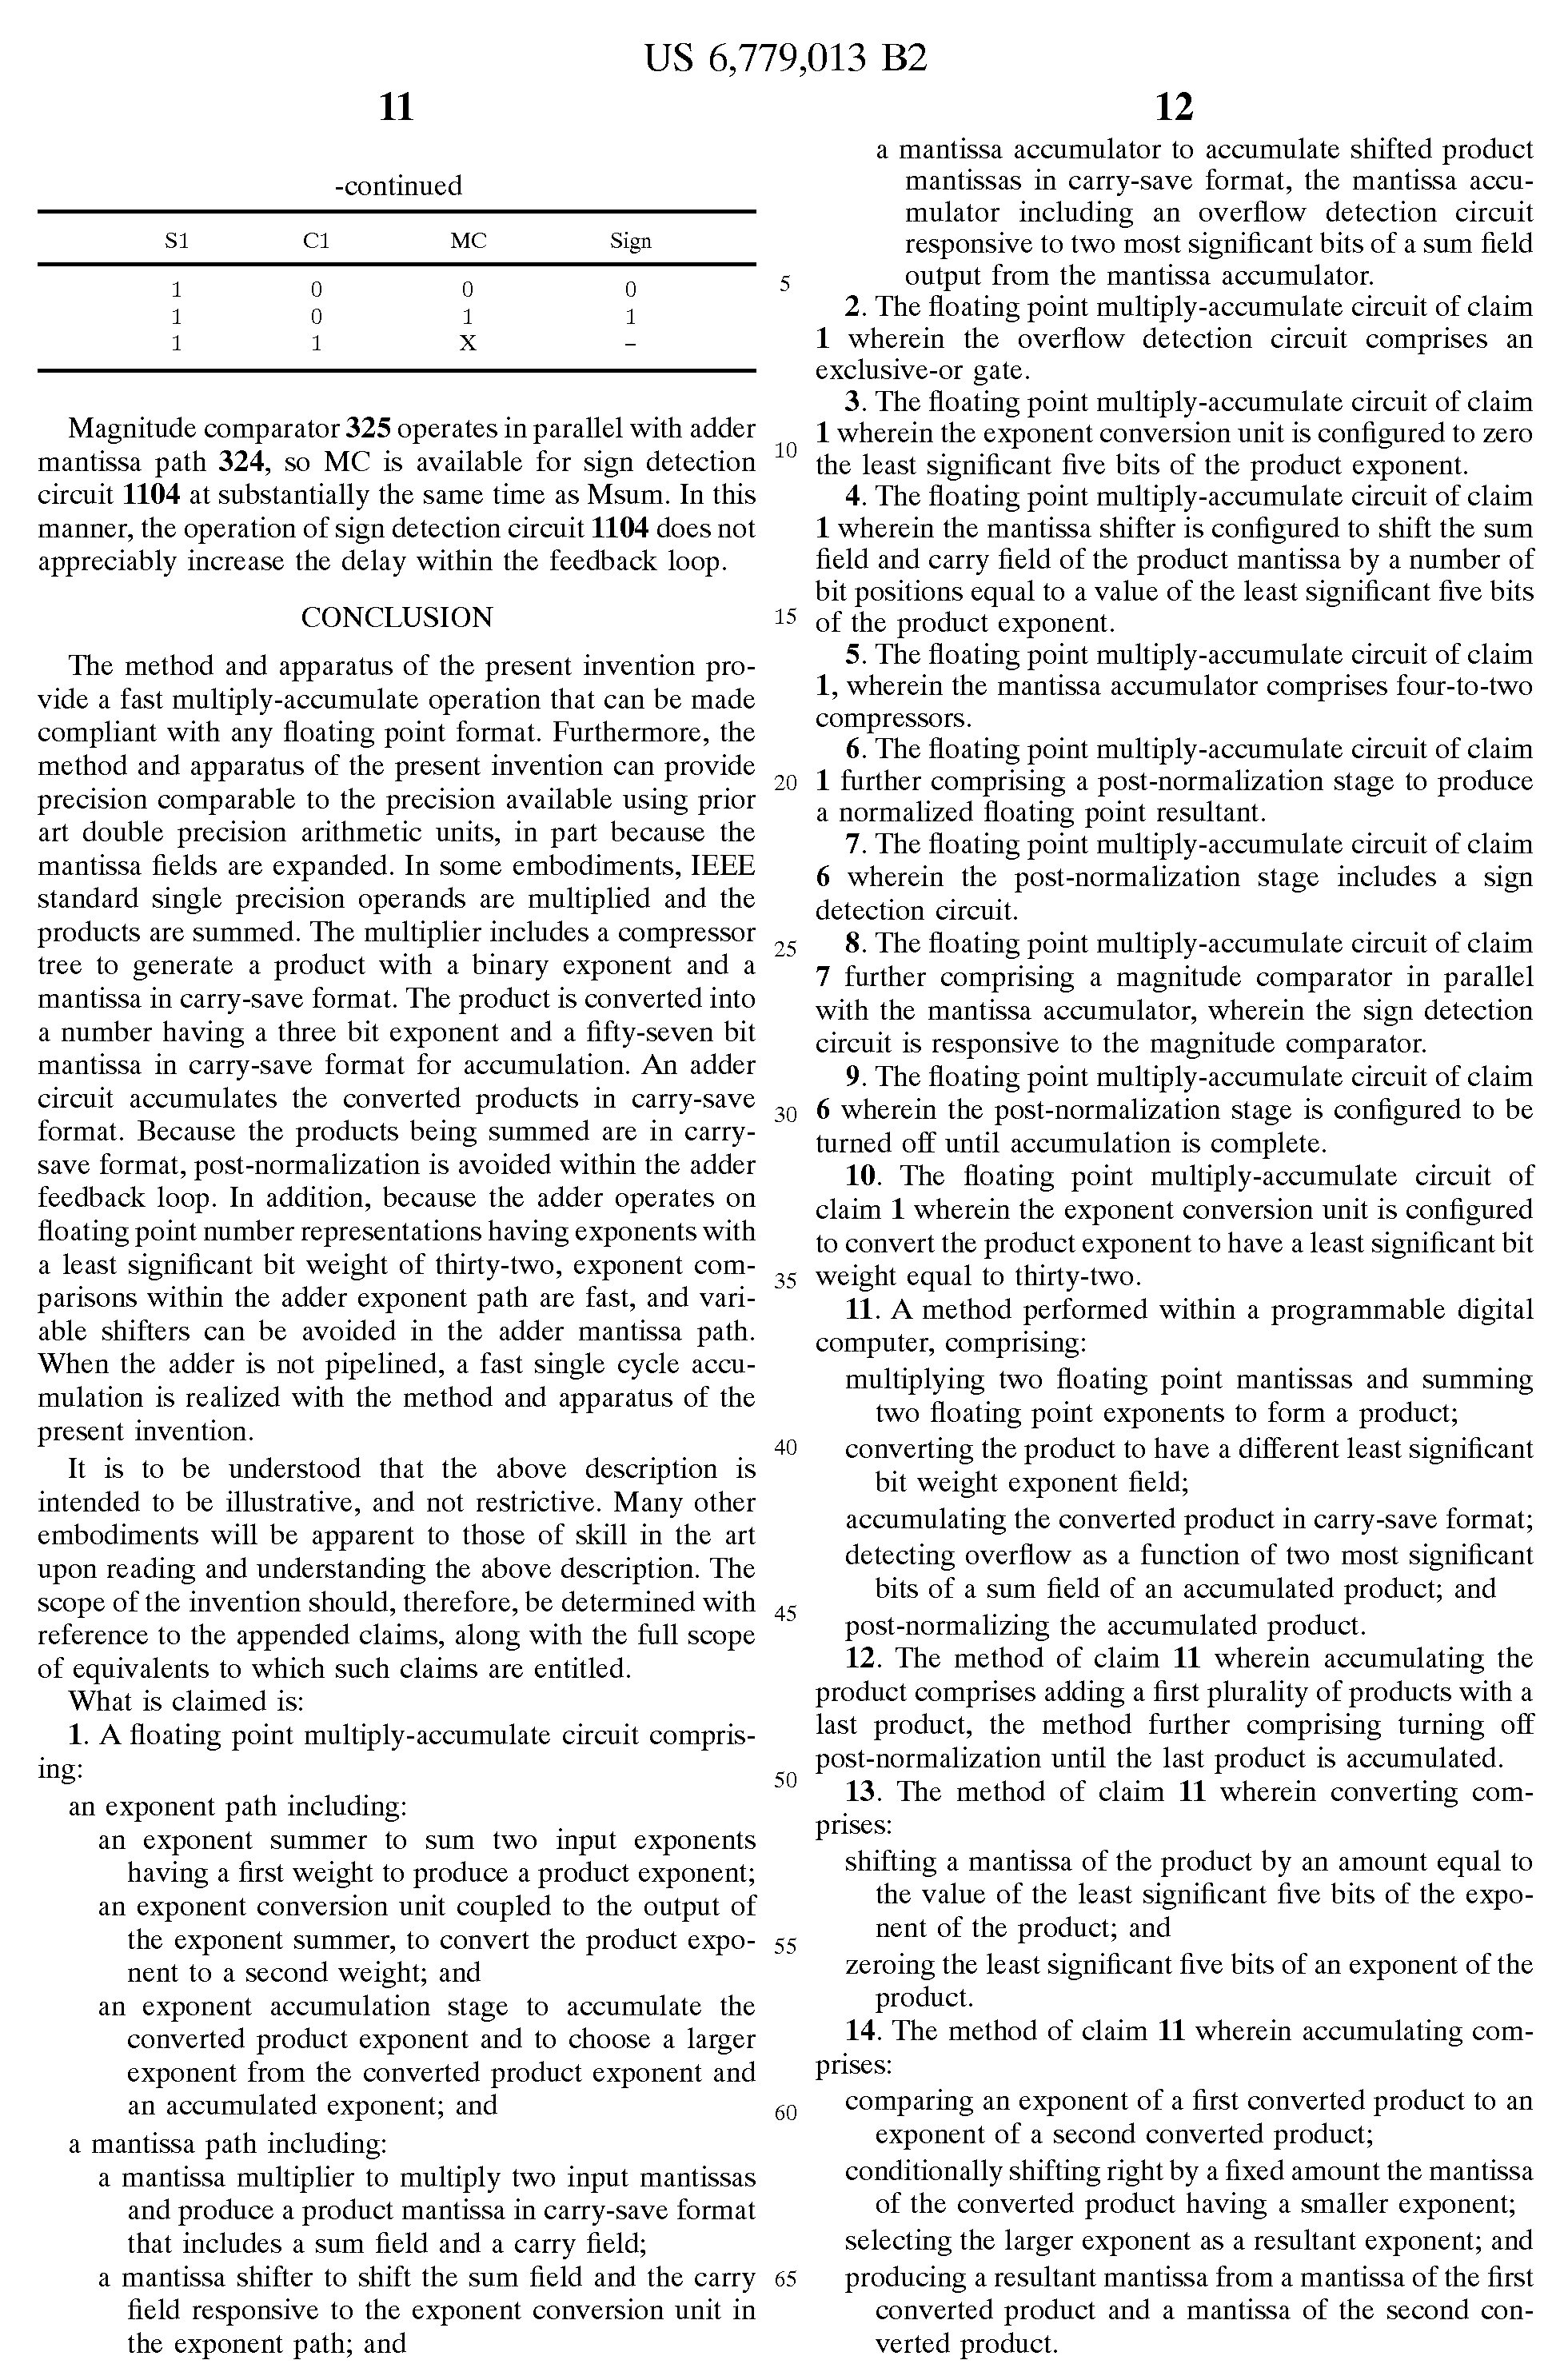
\includegraphics[width=4.14583in,height=0.8125in]{media/image3.emf}

\textbf{Figure 5.2} Level 0 audio power amplifier functionality.

The system should be described in as much detail as possible for each
level via the functional requirement. The Level 0 functional requirement
for this design is as follows.

\begin{longtable}[]{@{}
  >{\raggedright\arraybackslash}p{(\columnwidth - 2\tabcolsep) * \real{0.2068}}
  >{\raggedright\arraybackslash}p{(\columnwidth - 2\tabcolsep) * \real{0.7932}}@{}}
\toprule\noalign{}
\begin{minipage}[b]{\linewidth}\raggedright
\emph{Module}
\end{minipage} & \begin{minipage}[b]{\linewidth}\raggedright
Audio Power Amplifier
\end{minipage} \\
\midrule\noalign{}
\endhead
\bottomrule\noalign{}
\endlastfoot
\emph{Inputs} & \begin{minipage}[t]{\linewidth}\raggedright
\begin{itemize}
\item
  Audio input signal: 0.5V peak.
\item
  Power: 120 volts AC rms, 60Hz.
\item
  User volume control: variable control.
\end{itemize}
\end{minipage} \\
\emph{Outputs} & \begin{minipage}[t]{\linewidth}\raggedright
\begin{itemize}
\item
  Audio output signal: \ul{?}V peak value.
\end{itemize}
\end{minipage} \\
\emph{Functionality} & Amplify the input signal to produce a 50W maximum
output signal. The amplification should have variable user control. The
output volume should be variable between no volume and a maximum volume
level. \\
\end{longtable}

Not all values can be known on the first pass through the design as was
indicated in the guidelines. Underlined items represent values that need
to be determined or refined as the design proceeds. In this case, the
peak value of the audio output voltage is determined from the system
requirements on power gain. Knowing that the maximum power is given by
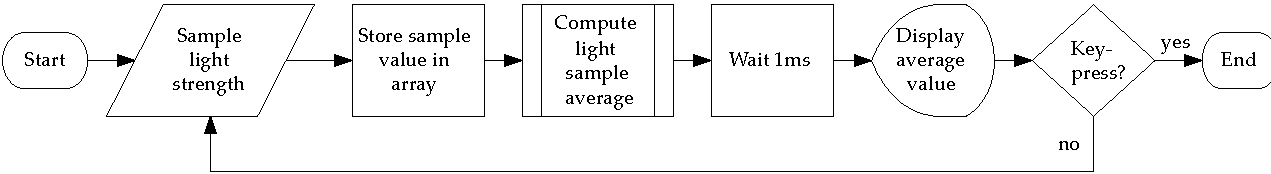
\includegraphics{media/image4.wmf}, allows the maximum output voltage to
be computed as 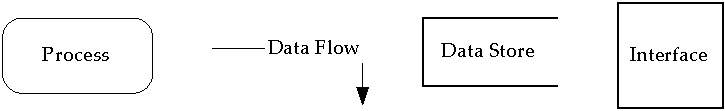
\includegraphics{media/image5.wmf}20V.

\subsubsection*{Level 1}\label{level-1}
\addcontentsline{toc}{subsubsection}{Level 1}

The Level 1 diagram, or system architecture, is shown in Figure 5.3.
This architecture is common in amplifier design and is but one possible
solution. It contains three cascaded amplifier stages and a DC supply
that powers the three stages. The first amplifier stage, the
\emph{buffer amplifier}, provides a high resistance buffer that
minimizes loading effects with the source. Buffer amplifiers have
extremely high input resistance and a unity signal gain. The \emph{high
gain amplifier} increases the amplitude of the signal, but provides
little in terms of the output current necessary to drive the speakers.
The last stage in the cascade is the \emph{power output stage}, which
provides the current needed to drive the speakers, but has no voltage
amplification.


\includegraphics[width=5.47917in,height=2.53125in]{media/image6.emf}

\textbf{Figure 5.3} Level 1 audio amplifier design.

The functional requirements for the Level 1 subsystems are now detailed,
starting with the buffer amplifier.

\begin{longtable}[]{@{}
  >{\raggedright\arraybackslash}p{(\columnwidth - 2\tabcolsep) * \real{0.2036}}
  >{\raggedright\arraybackslash}p{(\columnwidth - 2\tabcolsep) * \real{0.7964}}@{}}
\toprule\noalign{}
\begin{minipage}[b]{\linewidth}\raggedright
\emph{Module}
\end{minipage} & \begin{minipage}[b]{\linewidth}\raggedright
Buffer Amplifier
\end{minipage} \\
\midrule\noalign{}
\endhead
\bottomrule\noalign{}
\endlastfoot
\emph{Inputs} & \begin{minipage}[t]{\linewidth}\raggedright
\begin{itemize}
\item
  Audio input signal: 0.5V peak.
\item
  Power: ± \ul{25}V DC.
\end{itemize}
\end{minipage} \\
\emph{Outputs} & \begin{minipage}[t]{\linewidth}\raggedright
\begin{itemize}
\item
  Audio signal: 0.5V peak.
\end{itemize}
\end{minipage} \\
\emph{Functionality} & Buffer the input signal and provide unity voltage
gain. It should have an input resistance \textgreater{}\ul{1M}Ω and an
output resistance \textless{}\ul{100}Ω. \\
\end{longtable}

Where did the ± 25V DC value for the DC input power come from? The
system must produce a ± 20V AC output signal to satisfy the Level 0
requirement, so supply values that exceed that are required to power the
electronics. How about the values for the input and output resistance?
They are educated guesses, based on knowledge of what is achievable with
the technology (bottom-up knowledge). The exact resistance requirements
are refined later based upon the overall design, taking into account the
input and output resistances for all stages.

Now consider the functional requirements for the high gain amplifier.

\begin{longtable}[]{@{}
  >{\raggedright\arraybackslash}p{(\columnwidth - 2\tabcolsep) * \real{0.2036}}
  >{\raggedright\arraybackslash}p{(\columnwidth - 2\tabcolsep) * \real{0.7964}}@{}}
\toprule\noalign{}
\begin{minipage}[b]{\linewidth}\raggedright
\emph{Module}
\end{minipage} & \begin{minipage}[b]{\linewidth}\raggedright
High Gain Amplifier
\end{minipage} \\
\midrule\noalign{}
\endhead
\bottomrule\noalign{}
\endlastfoot
\emph{Inputs} & \begin{minipage}[t]{\linewidth}\raggedright
\begin{itemize}
\item
  Audio input signal: 0.5V peak.
\item
  User volume control: variable control.
\item
  Power: ± \ul{25}V DC
\end{itemize}
\end{minipage} \\
\emph{Outputs} & \begin{minipage}[t]{\linewidth}\raggedright
\begin{itemize}
\item
  Audio signal: \ul{20}V peak.
\end{itemize}
\end{minipage} \\
\emph{Functionality} & Provide an adjustable voltage gain, between \ul{1
and 40}. It should have an input resistance \textgreater{}\ul{100k}Ω and
an output resistance \textless{}\ul{100}Ω. \\
\end{longtable}

The gain of 40 is determined from the overall system power and gain
requirements (the maximum input voltage of 0.5V must be able to be
amplified to 20V), while the resistances are again educated guesses.

Now consider the power output stage.

\begin{longtable}[]{@{}
  >{\raggedright\arraybackslash}p{(\columnwidth - 2\tabcolsep) * \real{0.2071}}
  >{\raggedright\arraybackslash}p{(\columnwidth - 2\tabcolsep) * \real{0.7929}}@{}}
\toprule\noalign{}
\begin{minipage}[b]{\linewidth}\raggedright
\emph{Module}
\end{minipage} & \begin{minipage}[b]{\linewidth}\raggedright
Power Output Stage
\end{minipage} \\
\midrule\noalign{}
\endhead
\bottomrule\noalign{}
\endlastfoot
\emph{Inputs} & \begin{minipage}[t]{\linewidth}\raggedright
\begin{itemize}
\item
  Audio input signal: \ul{20}V peak.
\item
  Power: ± \ul{25}V DC.
\end{itemize}
\end{minipage} \\
\emph{Outputs} & \begin{minipage}[t]{\linewidth}\raggedright
\begin{itemize}
\item
  Audio signal: \ul{20}V peak at up to \ul{2.5}A.
\end{itemize}
\end{minipage} \\
\emph{Functionality} & Provide unity voltage gain with output current as
required by a resistive load of up to \ul{2.5}A. It should have an input
resistance \textgreater{}\ul{1M}Ω and output resistance
\textless{}\ul{1}Ω. \\
\end{longtable}

For the power output stage, it is clear that 20V peak needs to be
delivered, but how was the requirement on current determined? The
current needed to drive the speaker is determined from Ohm's Law as
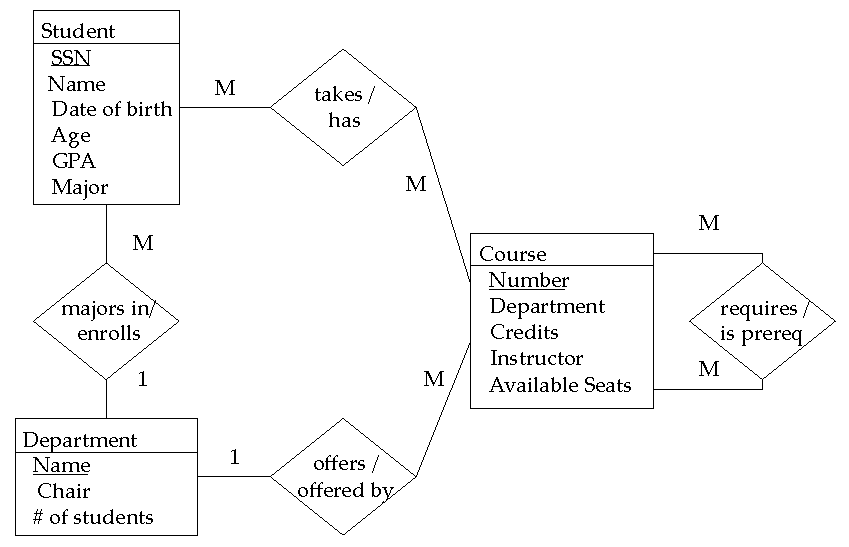
\includegraphics{media/image7.wmf}.

The last module to examine at this level is the power supply.

\begin{longtable}[]{@{}
  >{\raggedright\arraybackslash}p{(\columnwidth - 2\tabcolsep) * \real{0.2071}}
  >{\raggedright\arraybackslash}p{(\columnwidth - 2\tabcolsep) * \real{0.7929}}@{}}
\toprule\noalign{}
\begin{minipage}[b]{\linewidth}\raggedright
\emph{Module}
\end{minipage} & \begin{minipage}[b]{\linewidth}\raggedright
Power Supply
\end{minipage} \\
\midrule\noalign{}
\endhead
\bottomrule\noalign{}
\endlastfoot
\emph{Inputs} & \begin{minipage}[t]{\linewidth}\raggedright
\begin{itemize}
\item
  120 Volts AC rms.
\end{itemize}
\end{minipage} \\
\emph{Outputs} & \begin{minipage}[t]{\linewidth}\raggedright
\begin{itemize}
\item
  Power: ± \ul{25}V DC with up to \ul{3.0} A of current with a
  regulation of \textless{}\ul{1}\%.
\end{itemize}
\end{minipage} \\
\emph{Functionality} & Convert AC wall outlet voltage to positive and
negative DC output voltages, and provide enough current to drive all
amplifiers. \\
\end{longtable}

It is clear that the power supply needs to deliver ± 25V DC, while the
3.0A current capability was selected to supply the 2.5A needed for the
peak output power requirement plus the current needed to power the other
amplifier stages.

Finally, it is necessary to determine if the values of the input and
output resistances selected for the stages are realistic. For cascaded
amplifier stages, the overall voltage gain is given by the product of
gains multiplied by the voltage divider losses between stages
{[}Sed04{]}. In this case the overall gain is

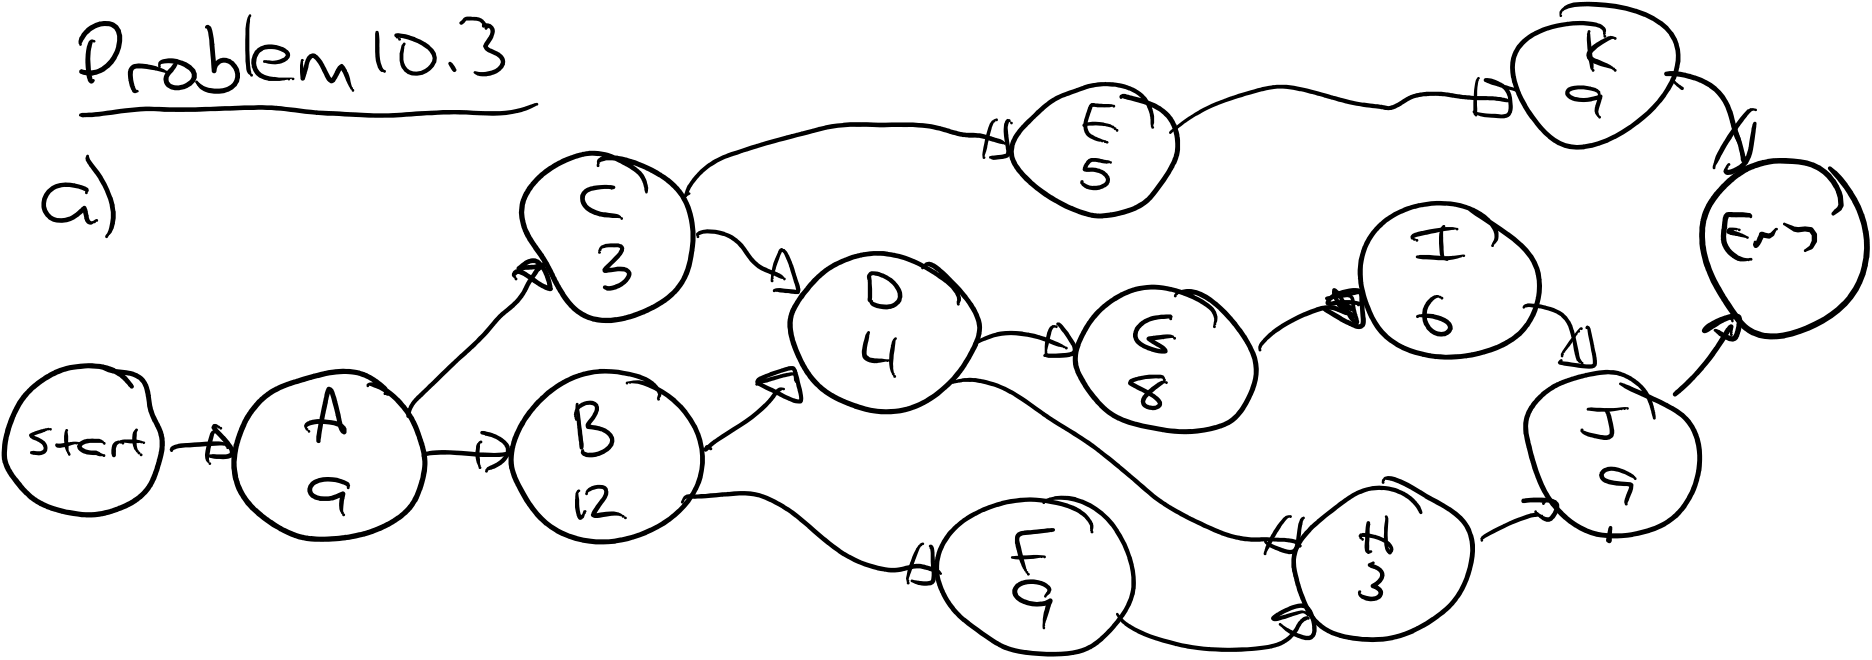
\includegraphics{media/image8.wmf}. (1)

So the resistance values selected in the functional requirements satisfy
the overall system requirements. If not, it would be necessary to go
back and refine them.

\subsubsection*{Level 2}\label{level-2}
\addcontentsline{toc}{subsubsection}{Level 2}

At this point, the three amplifier stages are ready for detailed
component level design, while the power supply needs another level of
refinement as shown in Figure 5.4. The functional requirement for each
of the elements in the power supply would be developed similarly.
Functional decomposition stops at this point---all levels of the
hierarchy are defined and the next step is the detailed design, where
the actual circuit components are determined.


\includegraphics[width=5.48958in,height=0.85417in]{media/image9.emf}

\textbf{Figure 5.4} Level 2 design of the power supply.

\subsection{Application: Digital
Design}\label{application-digital-design}

Functional decomposition is widely applied to the design of digital
systems, where it is known as \emph{entity-architecture} design. The
inputs and outputs refer to the entity, and the architecture describes
the functionality. The application of functional decomposition to
digital systems is demonstrated in the following example. Consider the
design of a simple digital stopwatch that keeps track of seconds and has
the following engineering requirements.

The system must

\begin{itemize}
\item
  Have no more than two control buttons.
\item
  Implement Run, Stop, and Reset functions.
\item
  Output a 16-bit binary number that represents seconds elapsed.
\end{itemize}

\subsubsection*{Level 0}\label{level-0-1}
\addcontentsline{toc}{subsubsection}{Level 0}

The Level 0 diagram and functional requirements are shown below.

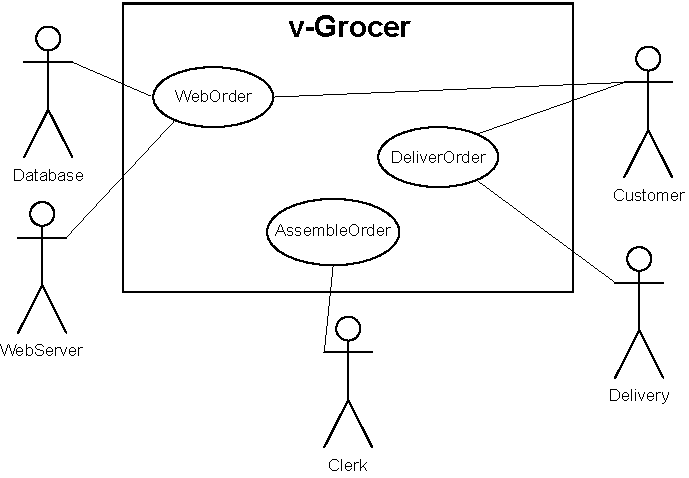
\includegraphics[width=2.6875in,height=0.95833in]{media/image10.emf}

\textbf{Figure 5.5} Level 0 digital stopwatch functionality.

\begin{longtable}[]{@{}
  >{\raggedright\arraybackslash}p{(\columnwidth - 2\tabcolsep) * \real{0.2034}}
  >{\raggedright\arraybackslash}p{(\columnwidth - 2\tabcolsep) * \real{0.7966}}@{}}
\toprule\noalign{}
\begin{minipage}[b]{\linewidth}\raggedright
\emph{Module}
\end{minipage} & \begin{minipage}[b]{\linewidth}\raggedright
Stopwatch
\end{minipage} \\
\midrule\noalign{}
\endhead
\bottomrule\noalign{}
\endlastfoot
\emph{Inputs} & \begin{minipage}[t]{\linewidth}\raggedright
\begin{itemize}
\item
  A: Reset button signal. When the button is pushed it resets the
  counter to zero.
\item
  B: Run/stop toggle signal. When the button is pushed it toggles
  between run and stop modes.
\end{itemize}
\end{minipage} \\
\emph{Outputs} & \begin{minipage}[t]{\linewidth}\raggedright
\begin{itemize}
\item
  b\textsubscript{15}-b\textsubscript{0}: 16-bit binary number that
  represents the number of seconds elapsed.
\end{itemize}
\end{minipage} \\
\emph{Functionality} & The stopwatch counts the number of seconds after
B is pushed when the system is in the Reset or Stop mode. When in Run
mode and B is pushed, the stopwatch stops counting. A reset button push
(A) will reset the output value of the counter to zero only when in Stop
mode. \\
\end{longtable}

\subsubsection*{Level 1}\label{level-1-1}
\addcontentsline{toc}{subsubsection}{Level 1}

The Level 1 architecture in Figure 5.6 contains three modules: a seconds
counter, a clock divider, and a finite state machine (FSM). The
stopwatch counts seconds, thus the seconds counter module counts the
seconds and outputs a 16-bit number representing the number of seconds
elapsed. The clock divider generates a 1Hz signal that triggers the
seconds counter. The FSM responds to the button press stimuli and
produces the appropriate control signals for the seconds counter. The
system clock is included to clock both the FSM and the clock divider.

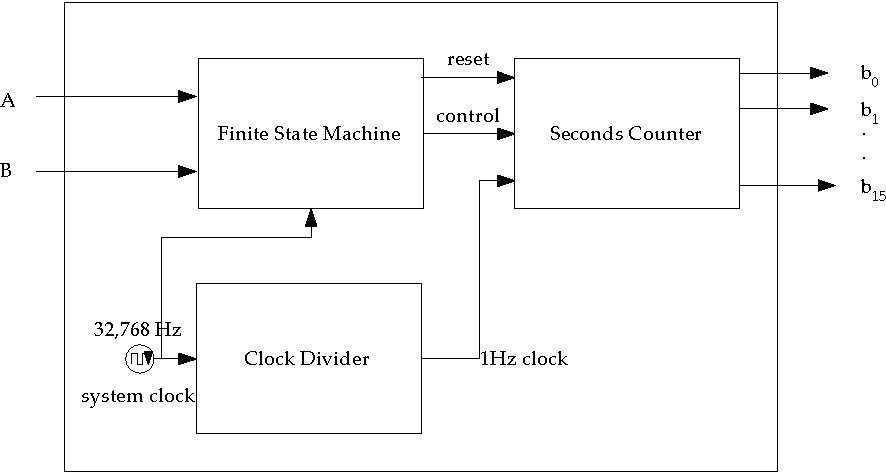
\includegraphics[width=5.5in,height=2.94792in]{media/image11.emf}

\textbf{Figure 5.6} Level 1 design for the digital stopwatch.

The functionality of the Level 1 modules is described as follows,
starting with the finite state machine.

\begin{longtable}[]{@{}
  >{\raggedright\arraybackslash}p{(\columnwidth - 2\tabcolsep) * \real{0.1966}}
  >{\raggedright\arraybackslash}p{(\columnwidth - 2\tabcolsep) * \real{0.8034}}@{}}
\toprule\noalign{}
\begin{minipage}[b]{\linewidth}\raggedright
\emph{Module}
\end{minipage} & \begin{minipage}[b]{\linewidth}\raggedright
Finite State Machine
\end{minipage} \\
\midrule\noalign{}
\endhead
\bottomrule\noalign{}
\endlastfoot
\emph{Inputs} & \begin{minipage}[t]{\linewidth}\raggedright
\begin{itemize}
\item
  A: Signal to reset the counter.
\item
  B: Signal to toggle the stopwatch between run and stop modes.
\item
  Clock: 1Hz clock signal.
\end{itemize}
\end{minipage} \\
\emph{Outputs} & \begin{minipage}[t]{\linewidth}\raggedright
\begin{itemize}
\item
  Reset: Signal to reset the counter to zero.
\item
  Control: Signal that enables or disables the counter.
\end{itemize}
\end{minipage} \\
\emph{Functionality} &

\includegraphics[width=1.98958in,height=1.1875in]{media/image12.emf} \\
\end{longtable}

The functionality of the finite state machine is described with a tool
that is probably familiar to the reader, the state diagram. State
diagrams are covered in more detail in Chapter 6. The state diagram
describes stimulus-response behavior, and shows how the system
transitions between states based upon logic signals from the button
presses.

Next, consider the clock divider.

\begin{longtable}[]{@{}
  >{\raggedright\arraybackslash}p{(\columnwidth - 2\tabcolsep) * \real{0.2071}}
  >{\raggedright\arraybackslash}p{(\columnwidth - 2\tabcolsep) * \real{0.7929}}@{}}
\toprule\noalign{}
\begin{minipage}[b]{\linewidth}\raggedright
\emph{Module}
\end{minipage} & \begin{minipage}[b]{\linewidth}\raggedright
Clock Divider
\end{minipage} \\
\midrule\noalign{}
\endhead
\bottomrule\noalign{}
\endlastfoot
\emph{Inputs} & \begin{minipage}[t]{\linewidth}\raggedright
\begin{itemize}
\item
  System clock: \ul{32,768}Hz.
\end{itemize}
\end{minipage} \\
\emph{Outputs} & \begin{minipage}[t]{\linewidth}\raggedright
\begin{itemize}
\item
  Internal clock: 1Hz clock for seconds elapsed.
\end{itemize}
\end{minipage} \\
\emph{Functionality} & Divide the system clock by 32,768 to produce a
1Hz clock. \\
\end{longtable}

The value of 32,768 Hz was selected for the system clock for several
reasons. It is a power of 2 that is easily divisible by digital
circuitry to produce a 1Hz output signal. It is also well above the
clock rate needed for detecting button presses and there is a wide
selection of crystals that can meet this requirement.

Finally, consider the seconds counter.

\begin{longtable}[]{@{}
  >{\raggedright\arraybackslash}p{(\columnwidth - 2\tabcolsep) * \real{0.2051}}
  >{\raggedright\arraybackslash}p{(\columnwidth - 2\tabcolsep) * \real{0.7949}}@{}}
\toprule\noalign{}
\begin{minipage}[b]{\linewidth}\raggedright
\emph{Module}
\end{minipage} & \begin{minipage}[b]{\linewidth}\raggedright
Seconds Counter
\end{minipage} \\
\midrule\noalign{}
\endhead
\bottomrule\noalign{}
\endlastfoot
\emph{Inputs} & \begin{minipage}[t]{\linewidth}\raggedright
\begin{itemize}
\item
  Reset: Reset the counter to zero.
\item
  Control: Enable/disable the counter.
\item
  Clock: Increment the counter.
\end{itemize}
\end{minipage} \\
\emph{Outputs} & \begin{minipage}[t]{\linewidth}\raggedright
\begin{itemize}
\item
  b\textsubscript{15}-b\textsubscript{0}: 16-bit binary representation
  of number of seconds elapsed.
\end{itemize}
\end{minipage} \\
\emph{Functionality} & Count the seconds when enabled and resets to zero
when reset signal enabled. \\
\end{longtable}

The system decomposition would end here, assuming that the design is to
be implemented using off-the-shelf chips. The next step would be to
determine components at the detailed design level. However, if it were
an integrated circuit design, the description would continue until the
transistor level is reached.

\subsection{Application: Software
Design}\label{application-software-design}

Software also lends itself to functional decomposition since virtually
all computing languages provide the capability to call functions,
subroutines, or modules. Functional software design simplifies program
development by eliminating the need to create redundant code via the use
of functions that are called repeatedly.

\emph{\textbf{Structure charts}} are specialized block diagrams for
visualizing functional software designs. The modules used in a structure
chart are shown in Figure 5.7. The larger arrows indicate connections to
other modules, while the smaller arrows represent data and control
information passed between modules. Five basic modules are utilized:

\begin{enumerate}
\def\labelenumi{\arabic{enumi}.}
\item
  \emph{Input} \emph{modules}. Receive information.
\item
  \emph{Output} \emph{modules.} Return information.
\item
  \emph{Transform} \emph{modules.} Receive information, change it, and
  return the changed information.
\item
  \emph{Coordination} \emph{modules.} Coordinate or synchronize
  activities between modules.
\item
  \emph{Composite} \emph{modules.} Any possible combination of the other
  four.
\end{enumerate}

This approach to software design, also known as \emph{structured
design}, was formalized in the 1970's by IBM researchers {[}Ste99{]}.


\includegraphics[width=5.5in,height=1.40625in]{media/image13.emf}

\textbf{Figure 5.7} Module types for functional software design. The
larger arrows indicate connections between modules and the smaller
arrows represent data and control.

The following example demonstrates the application of functional
decomposition to a software design with the following requirements.

The system must

\begin{itemize}
\item
  Accept an ASCII file of integer numbers as input.
\item
  Sort the numbers into ascending order and save the sorted numbers to
  disk.
\item
  Compute the mean of the numbers.
\item
  Display the mean on the screen.
\end{itemize}

This is a fairly simple task that could easily be done in a single
function, but doing so would not allow components of the design to be
easily reused, tested, or troubleshot. The engineering requirements
themselves provide some guidance in terms of how to arrange the
functionality of the modules (\emph{form follows function}). The
architecture in Figure 5.8 contains a main module that calls three
sub-modules. In this design main is a coordinating module that controls
the processing and calling of the other modules, a common scenario. It
was also decided that all user interaction would take place within main.
The order of the processing is not described by structure charts. In our
program, main calls ReadArray, SortArray, and ComputeMean in sequential
order. main passes the filename (fname) to ReadArray, which reads in the
array and the number of elements in it, and returns this information to
main. The choice of passing in the filename was deliberate; the user
could have been prompted for the filename in ReadArray, but doing so
might limit future reuse of the function since you may not always want
to do so when reading an array of data. SortArray is then called, which
accepts the array of numbers and the number of elements in the array,
and returns the sorted values in the same array. Finally, ComputeMean is
executed, which accepts the sorted array and the number of elements,
computes the mean value, and returns it to main.

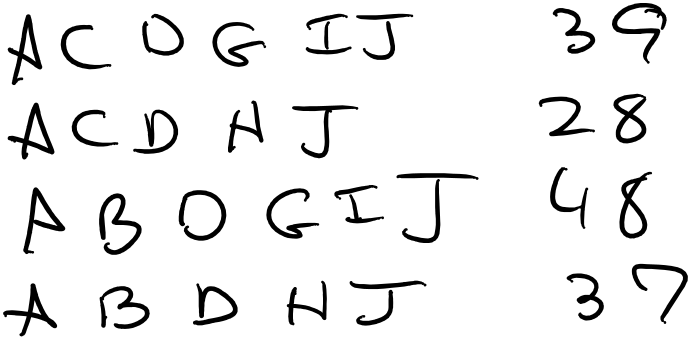
\includegraphics[width=4.13542in,height=1.89583in]{media/image14.emf}

\textbf{Figure 5.8} Structure chart design of sorting and mean
computation program.

The functional requirements for each module in the structure chart are
detailed in Table 5.1. The structure chart provides a visual
relationship between modules in the design, but also has some
disadvantages. It is difficult to visualize designs as the complexity of
the software increases. This can be addressed by expanding sublevels in
the design as necessary in different diagrams. Structure charts also
lack a temporal aspect that indicates the calling order. Most software
systems have many layers in the hierarchy and highly complex calling
patterns. In this example, main calls three modules in a well-defined
order, but if there was another level in the hierarchy, there is no
reason why it could not be called by a module at any other level. That
leads to some of the unique problems associated with software design.
Functional design works well for small-to-moderately complex software,
but tends to fall short when applied to large scale software systems. As
such, it has given way to the object-oriented design approach.

\subsection{Application: Thermometer
Design}\label{application-thermometer-design}

The final example includes both analog and digital modules where the
objective is to design a thermometer that meets the following
engineering requirements.

The system must

\begin{itemize}
\item
  Measure temperature between 0 and 200°C.
\item
  Have an accuracy of 0.4\% of full scale.
\item
  Display the temperature digitally, including one digit beyond the
  decimal point.
\item
  Be powered by a standard 120V 60Hz AC outlet.
\item
  Use an RTD (thermal resistive device) that has an accuracy of 0.55°C
  over the range. The resistance of the RTD varies linearly with
  temperature from 100Ω at 0°C to 178Ω at 200°C. (Note: this requirement
  does not meet the abstractness property identified in Chapter 3, since
  it identifies part of the solution. This requirement is given to
  provide guidance in this example.)

  \textbf{Table 5.1} Functional design requirements for the number sort
  program.
\end{itemize}

\subsubsection*{\texorpdfstring{\hfill\break
Level 0}{ Level 0}}\label{level-0-2}
\addcontentsline{toc}{subsubsection}{\hfill\break
Level 0}

\begin{longtable}[]{@{}
  >{\raggedright\arraybackslash}p{(\columnwidth - 2\tabcolsep) * \real{0.2358}}
  >{\raggedright\arraybackslash}p{(\columnwidth - 2\tabcolsep) * \real{0.7642}}@{}}
\toprule\noalign{}
\begin{minipage}[b]{\linewidth}\raggedright
\emph{Module name}
\end{minipage} & \begin{minipage}[b]{\linewidth}\raggedright
main()
\end{minipage} \\
\midrule\noalign{}
\endhead
\bottomrule\noalign{}
\endlastfoot
\emph{Module type} & Coordination \\
\emph{Input arguments} & None \\
\emph{Output arguments} & None \\
\emph{Description} & The main function calls ReadArray() to read the
input file from disk, SortArray() to sort the array, and ComputeMean()
to determine the mean value of elements in the array. User interaction
requires the user to enter the filename, and the mean value is displayed
on the screen. \\
\emph{Modules invoked} & ReadArray, SortArray, and ComputeMean \\
\end{longtable}

\begin{longtable}[]{@{}
  >{\raggedright\arraybackslash}p{(\columnwidth - 2\tabcolsep) * \real{0.2445}}
  >{\raggedright\arraybackslash}p{(\columnwidth - 2\tabcolsep) * \real{0.7555}}@{}}
\toprule\noalign{}
\begin{minipage}[b]{\linewidth}\raggedright
\emph{Module name}
\end{minipage} & \begin{minipage}[b]{\linewidth}\raggedright
ReadArray()
\end{minipage} \\
\midrule\noalign{}
\endhead
\bottomrule\noalign{}
\endlastfoot
\emph{Module type} & Input and output \\
\emph{Input arguments} & \begin{minipage}[t]{\linewidth}\raggedright
\begin{itemize}
\item
  fname{[}{]}: character array with filename to read from.
\end{itemize}
\end{minipage} \\
\emph{Output Arguments} & \begin{minipage}[t]{\linewidth}\raggedright
\begin{itemize}
\item
  numArray{[}{]}: integer array with elements read from file.
\item
  N: number of elements in numArray{[}{]}.
\end{itemize}
\end{minipage} \\
\emph{Description} & Read data from input data file and store elements
in array numArray{[}{]}. The number of elements read is placed in N. \\
\emph{Modules invoked} & None \\
\end{longtable}

\begin{longtable}[]{@{}
  >{\raggedright\arraybackslash}p{(\columnwidth - 2\tabcolsep) * \real{0.2453}}
  >{\raggedright\arraybackslash}p{(\columnwidth - 2\tabcolsep) * \real{0.7547}}@{}}
\toprule\noalign{}
\begin{minipage}[b]{\linewidth}\raggedright
\emph{Module name}
\end{minipage} & \begin{minipage}[b]{\linewidth}\raggedright
SortArray()
\end{minipage} \\
\midrule\noalign{}
\endhead
\bottomrule\noalign{}
\endlastfoot
\emph{Module type} & Transformation \\
\emph{Input arguments} & \begin{minipage}[t]{\linewidth}\raggedright
\begin{itemize}
\item
  numArray{[}{]}: integer array of numbers.
\item
  N: number of elements in numArray{[}{]}.
\end{itemize}
\end{minipage} \\
\emph{Output Arguments} & \begin{minipage}[t]{\linewidth}\raggedright
\begin{itemize}
\item
  numArray{[}{]}: sorted array of integer numbers.
\end{itemize}
\end{minipage} \\
\emph{Description} & Sort elements in array using a shell sort
algorithm. Saves the the sorted array to disk. \\
\emph{Modules invoked} & None \\
\end{longtable}

\begin{longtable}[]{@{}
  >{\raggedright\arraybackslash}p{(\columnwidth - 2\tabcolsep) * \real{0.2445}}
  >{\raggedright\arraybackslash}p{(\columnwidth - 2\tabcolsep) * \real{0.7555}}@{}}
\toprule\noalign{}
\begin{minipage}[b]{\linewidth}\raggedright
\emph{Module name}
\end{minipage} & \begin{minipage}[b]{\linewidth}\raggedright
ComputeMean()
\end{minipage} \\
\midrule\noalign{}
\endhead
\bottomrule\noalign{}
\endlastfoot
\emph{Module type} & Input and output \\
\emph{Input arguments} & \begin{minipage}[t]{\linewidth}\raggedright
\begin{itemize}
\item
  numArray{[}{]}: integer array of numbers.
\item
  N: number of elements in numArray{[}{]}.
\end{itemize}
\end{minipage} \\
\emph{Output arguments} & \begin{minipage}[t]{\linewidth}\raggedright
\begin{itemize}
\item
  mean: mean value of the elements in the array.
\end{itemize}
\end{minipage} \\
\emph{Description} & Computes the mean value of the integer elements in
the array. \\
\emph{Modules invoked} & None \\
\end{longtable}

The overall goal is to convert a sensed temperature to a digital
temperature reading. The Level 0 description is as follows.

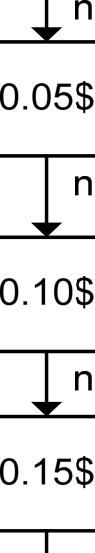
\includegraphics[width=3.39583in,height=0.875in]{media/image15.emf}

\textbf{Figure 5.9} Level 0 digital thermometer functionality.

\begin{longtable}[]{@{}
  >{\raggedright\arraybackslash}p{(\columnwidth - 2\tabcolsep) * \real{0.2032}}
  >{\raggedright\arraybackslash}p{(\columnwidth - 2\tabcolsep) * \real{0.7968}}@{}}
\toprule\noalign{}
\begin{minipage}[b]{\linewidth}\raggedright
\emph{Module}
\end{minipage} & \begin{minipage}[b]{\linewidth}\raggedright
Digital Thermometer
\end{minipage} \\
\midrule\noalign{}
\endhead
\bottomrule\noalign{}
\endlastfoot
\emph{Inputs} & \begin{minipage}[t]{\linewidth}\raggedright
\begin{itemize}
\item
  Ambient temperature: 0-200°C.
\item
  Power: 120V AC power.
\end{itemize}
\end{minipage} \\
\emph{Outputs} & \begin{minipage}[t]{\linewidth}\raggedright
\begin{itemize}
\item
  Digital temperature display: A four digit display, including one digit
  beyond the decimal point.
\end{itemize}
\end{minipage} \\
\emph{Functionality} & Displays temperature on digital readout with an
accuracy of 0.4\% of full scale. \\
\end{longtable}

\subsubsection*{Level 1}\label{level-1-2}
\addcontentsline{toc}{subsubsection}{Level 1}

The Level 1 architecture selected is shown in Figure 5.10. The
temperature conversion unit converts the temperature to an analog
voltage using the RTD that is sampled by the analog-to-digital
converter. The N-bit binary output from the converter is translated into
binary-coded decimal (BCD). BCD is a 4-bit representation of the digits
between 0 and 9. Since there are four display digits, there are four
separate binary encoded outputs from the BCD conversion unit. Common
7-segment LEDs are used for the display. However, they do not directly
accept BCD and instead have seven input lines, each of which is
individually switched to control the display segments. The requirements
did not specifically address cost or size constraints, nor clearly
define the environment, so there are many possible solutions. For
example, an analog-to-digital current converter could be used,
integrated circuit temperature sensing packages could be considered, and
microcontroller-based solutions are feasible as well.

From a system design perspective, an error budget is needed to identify
the maximum error that each subsystem may introduce, while still
achieving the overall accuracy. In this case, error is introduced in the
temperature conversion unit and A/D converter, but not in the remaining
digital components. The overall accuracy that the system must achieve is
0.4\%, and that translates into 0.8°C of allowable error for the 200°C
range. Let's now examine the modules.

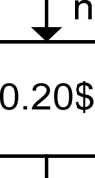
\includegraphics[width=5.47917in,height=1.83333in]{media/image16.emf}

\textbf{Figure 5.10} Level 1 design of the digital thermometer.

The functionality of the Level 1 modules is described as follows,
starting with the temperature conversion unit.

\begin{longtable}[]{@{}
  >{\raggedright\arraybackslash}p{(\columnwidth - 2\tabcolsep) * \real{0.2033}}
  >{\raggedright\arraybackslash}p{(\columnwidth - 2\tabcolsep) * \real{0.7967}}@{}}
\toprule\noalign{}
\begin{minipage}[b]{\linewidth}\raggedright
\emph{Module}
\end{minipage} & \begin{minipage}[b]{\linewidth}\raggedright
Temperature Conversion Unit
\end{minipage} \\
\midrule\noalign{}
\endhead
\bottomrule\noalign{}
\endlastfoot
\emph{Inputs} & \begin{minipage}[t]{\linewidth}\raggedright
\begin{itemize}
\item
  Ambient temperature: 0-200°C.
\item
  Power: \ul{?}V DC (to power the electronics).
\end{itemize}
\end{minipage} \\
\emph{Outputs} & \begin{minipage}[t]{\linewidth}\raggedright
\begin{itemize}
\item
  V\textsubscript{T}: temperature proportional voltage.
  V\textsubscript{T}= \ul{α}T, and ranges from \ul{?} to \ul{?}V.
\end{itemize}
\end{minipage} \\
\emph{Functionality} & Produces an output voltage that is linearly
proportional to temperature. It must achieve an accuracy of \ul{?}\%. \\
\end{longtable}

There are several unknowns at this point. The voltage necessary to power
the electronics is not known, but a reasonable assumption could be made.
The output voltage range and the accuracy are unknown. It is known that
the RTD will introduce up to 0.55°C of error and that the electronics
themselves will introduce additional error (the exact amount is unknown
at this point). An educated guess is made that the maximum error allowed
for the temperature unit is 0.6°C. This means that the electronics
themselves would be required to introduce no more than 0.05°C of error
due to the 0.55°C of error introduced by the RTD.

Now consider the analog to digital converter.

\begin{longtable}[]{@{}
  >{\raggedright\arraybackslash}p{(\columnwidth - 2\tabcolsep) * \real{0.2029}}
  >{\raggedright\arraybackslash}p{(\columnwidth - 2\tabcolsep) * \real{0.7971}}@{}}
\toprule\noalign{}
\begin{minipage}[b]{\linewidth}\raggedright
\emph{Module}
\end{minipage} & \begin{minipage}[b]{\linewidth}\raggedright
A/D Converter
\end{minipage} \\
\midrule\noalign{}
\endhead
\bottomrule\noalign{}
\endlastfoot
\emph{Inputs} & \begin{minipage}[t]{\linewidth}\raggedright
\begin{itemize}
\item
  V\textsubscript{T}: voltage proportional to temperature that ranges
  from \ul{?} to \ul{?}V.
\item
  Power: \ul{?}V DC.
\end{itemize}
\end{minipage} \\
\emph{Outputs} & \begin{minipage}[t]{\linewidth}\raggedright
\begin{itemize}
\item
  b\textsubscript{N-1} -b\textsubscript{0}: \ul{?-}bit binary
  representation of V\textsubscript{T}.
\end{itemize}
\end{minipage} \\
\emph{Functionality} & Converts analog input to binary digital
output. \\
\end{longtable}

The A/D converter is not likely to be something that is designed due to
the availability of low cost, off-the-shelf solutions. The requirements
drive the converter selection. There are two unknowns\emph{---}the
number of bits and the range of the input voltage. The number of bits
affects the accuracy, since the greater the number of bits, the better
the accuracy. The number of bits needed for the converter is calculated
from the maximum allowable error that the A/D can introduce (0.2°C), the
number of discrete intervals, and the temperate range as


\includegraphics{media/image17.wmf}. (2)

So the A/D converter needs to have at least 10 bits. How is the voltage
range selected? It is typically fixed for a particular integrated
circuit solution, but the temperature conversion subsystem output should
be matched to the voltage range so that all bits are effectively
utilized, otherwise, error is introduced.

Now, consider the BCD conversion unit.

\begin{longtable}[]{@{}
  >{\raggedright\arraybackslash}p{(\columnwidth - 2\tabcolsep) * \real{0.2029}}
  >{\raggedright\arraybackslash}p{(\columnwidth - 2\tabcolsep) * \real{0.7971}}@{}}
\toprule\noalign{}
\begin{minipage}[b]{\linewidth}\raggedright
\emph{Module}
\end{minipage} & \begin{minipage}[b]{\linewidth}\raggedright
BCD Conversion Unit
\end{minipage} \\
\midrule\noalign{}
\endhead
\bottomrule\noalign{}
\endlastfoot
\emph{Inputs} & \begin{minipage}[t]{\linewidth}\raggedright
\begin{itemize}
\item
  10-bit binary number (b\textsubscript{9}-b\textsubscript{0}):
  Represents the range 0.0-200.0°C.
\item
  Power: \ul{?}V DC.
\end{itemize}
\end{minipage} \\
\emph{Outputs} & \begin{minipage}[t]{\linewidth}\raggedright
\begin{itemize}
\item
  BCD\textsubscript{0}: 4-bit BCD representation of tenths digit (after
  decimal).
\item
  BCD\textsubscript{1}: 4-bit BCD representation of one's digit.
\item
  BCD\textsubscript{2}: 4-bit BCD representation of ten's digit.
\item
  BCD\textsubscript{3}: 4-bit BCD representation of hundred's digit.
\end{itemize}
\end{minipage} \\
\emph{Functionality} & Converts the 10-bit binary number to BCD
representation of temperature. Must refresh the displays twice a
second. \\
\end{longtable}

The objective of the BCD conversion unit is fairly simple, although the
component level design of the circuitry to accomplish the conversion is
not.

This leads to the last module, the 7-segment LED driver, whose
functionality is described as follows.

\begin{longtable}[]{@{}
  >{\raggedright\arraybackslash}p{(\columnwidth - 2\tabcolsep) * \real{0.2030}}
  >{\raggedright\arraybackslash}p{(\columnwidth - 2\tabcolsep) * \real{0.7970}}@{}}
\toprule\noalign{}
\begin{minipage}[b]{\linewidth}\raggedright
\emph{Module}
\end{minipage} & \begin{minipage}[b]{\linewidth}\raggedright
7-Segment LED Driver
\end{minipage} \\
\midrule\noalign{}
\endhead
\bottomrule\noalign{}
\endlastfoot
\emph{Inputs} & \begin{minipage}[t]{\linewidth}\raggedright
\begin{itemize}
\item
  BCD\textsubscript{0}: 4-bit BCD representation of tenths digit (after
  decimal).
\item
  BCD\textsubscript{1}: 4-bit BCD representation of one's digit.
\item
  BCD\textsubscript{2}: 4-bit BCD representation of ten's digit.
\end{itemize}

\begin{itemize}
\item
  BCD\textsubscript{3}: 4-bit BCD representation of hundred's digit.
\item
  Power: \ul{?}V DC.
\end{itemize}
\end{minipage} \\
\emph{Outputs} & \begin{minipage}[t]{\linewidth}\raggedright
\begin{itemize}
\item
  Four 7-segment driver lines.
\end{itemize}
\end{minipage} \\
\emph{Functionality} & Converts the BCD for each digit into outputs that
turn on LEDs in 7-segment package to display the temperature. \\
\end{longtable}

For completeness, the functional requirements of the power supply are
supplied. They are similar to the power supply requirements utilized in
the audio amplifier design in Section 5.4.

\begin{longtable}[]{@{}
  >{\raggedright\arraybackslash}p{(\columnwidth - 2\tabcolsep) * \real{0.2032}}
  >{\raggedright\arraybackslash}p{(\columnwidth - 2\tabcolsep) * \real{0.7968}}@{}}
\toprule\noalign{}
\begin{minipage}[b]{\linewidth}\raggedright
\emph{Module}
\end{minipage} & \begin{minipage}[b]{\linewidth}\raggedright
Power supply
\end{minipage} \\
\midrule\noalign{}
\endhead
\bottomrule\noalign{}
\endlastfoot
\emph{Inputs} & \begin{minipage}[t]{\linewidth}\raggedright
\begin{itemize}
\item
  120 Volts AC rms.
\end{itemize}
\end{minipage} \\
\emph{Outputs} & \begin{minipage}[t]{\linewidth}\raggedright
\begin{itemize}
\item
  ± \ul{?}V DC with up to \ul{?}mA of current.
\item
  Regulation of \ul{?}\%.
\end{itemize}
\end{minipage} \\
\emph{Functionality} & Convert AC wall outlet voltage to positive and
negative DC output voltages, with enough current to drive all circuit
subsystems. \\
\end{longtable}

At this point, the requirements for the major subsystems are completed
and ready for design at the component level. Illustration of the
complete design would require a fair amount of detail, and while it is
not presented here, some of the issues involved are discussed. First,
there are a variety of electronic circuits (inverting op amps, single
BJT configurations, and current mirrors, etc.---see Example 4.1 in
Chapter 4) that could be utilized as a current source to drive the RTD
in the temperature conversion subsystem. A midrange resolution A/D
converter is needed, and its particular input voltage range drives the
output voltage requirements for the temperature conversion module. The
BCD conversion circuitry could be implemented using combinational
digital logic (tedious due to the number of discrete gates), or a more
efficient, but slower, sequential logic design. Finally, the 7-segment
display converters could be designed using combinational logic that maps
the BCD inputs into outputs to activate the appropriate display
segments.

\subsection{Coupling and Cohesion}\label{coupling-and-cohesion}

The concepts of coupling and cohesion are examined before concluding
this chapter. They originated to describe software designs {[}Ste99{]},
but are applicable to electrical and computer systems. To understand
their importance, consider the relationship between the number of
modules in a system and the number of connections between them. For our
purposes, a connection between two modules may consist of any number of
signals without regard to their direction. Thus, a system consisting of
two modules has, at most, one connection. If the number of modules is
increased to three, the number of possible connections increases to
three, a system with four modules has six possible connections, and five
modules increases the number of possible connections to ten. The point
is that the maximum number of potential connections increases rapidly
with the number of modules in the system. The relationship between the
maximum possible connections and number of modules (\emph{n}) is given
by

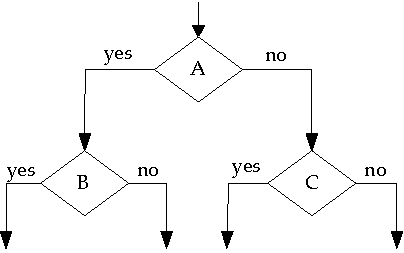
\includegraphics{media/image18.wmf}. (3)

Modules are coupled if they depend upon each other in some way to
operate properly. \emph{\textbf{Coupling}} is the extent to which
modules or subsystems are connected {[}Jal97{]}. Although there is no
agreed upon mathematical definition of coupling, it seems obvious that
increasing the exchange of control and data between two modules leads to
a higher degree of coupling. When systems are highly coupled, it is
difficult to change one module without impacting the other. Consider the
extreme case where all modules in a system are connected to each
other---an error in one module has the potential to impact every other
module in the system. Errors in a module are propagated to others to a
degree that is related to the amount of coupling. From this point of
view, it is good to minimize coupling. Yet coupling cannot be
eliminated, since the point of functional decomposition is to break a
design into components that work together to produce a higher level
behavior.

There are two ways to reduce coupling---minimize the number of
connections between modules and maximize cohesion within modules.
\emph{\textbf{Cohesion}} refers to how focused a module is---highly
cohesive systems do one or a few things very well. Stevens \emph{et al.}
{[}Ste99{]} defined six types of cohesion from the weakest to strongest
as: coincidental, logical, temporal, communicational, sequential, and
functional. More information on this can be found in the original work,
but the conclusion is that modules with high functional cohesion are the
most desirable. So it is best to design modules with a single
well-defined functional objective consistent with the philosophy of
functional decomposition. This leads to the important design principle
that it is desirable to maximize cohesion, while minimizing coupling.

Coupling and cohesion impact the later stages of testing and system
integration. If a particular module is highly cohesive, then it should
be possible to test it independently of the other modules to verify its
operability. This does not mean that it will necessarily operate
properly when integrated into the overall system, but the probability
that it will is higher if provided with proper inputs from connected
modules. Contrast this to the case of a low cohesion system. In that
case, it will likely be difficult to test the individual modules without
first integrating them.

To develop a better understanding, consider the amplifier design in
Figure 5.3 (Section 5.4) with three cascaded amplifier stages. Each
stage is highly cohesive, performing a singular function of signal
amplification. Each of these stages could easily operate as a
stand-alone module independent of the complete system. How about
coupling? In terms of the number of connections, it is fairly low as
each amplifier stage has an input and output voltage signal. The most
coupled module in the system is the power supply, and not surprisingly,
its failure leads to a complete system failure. Coupling in this case
can also be viewed in terms of the resistance matching between input and
output of the cascaded stages, producing the voltage divider effect in
equation (1). For voltage amplifiers, the goal is to have high input
resistance and low output resistance, which minimize both voltage losses
and coupling. The stages are not completely uncoupled, because the input
resistances, although large, are not infinite, and the output
resistances are not zero. The modules in the power supply unit in Figure
5.4 (rectifier, smoothing filter, and regulator) have a much higher
degree of coupling. In fact, it is difficult to develop a clear
functional decomposition of the power supply module because the elements
in the smoothing filter also serve as part of the rectifier circuit
(refer to a basic electronics textbook {[}Sed04{]} for more
information).

As another example, consider a software design where two options are
under consideration: one large function with 1000 lines of code, versus
15 cohesive functions, each with an average of 100 lines of code. Both
perform the same function, but which runs faster? Most likely the first,
as it would be highly integrated and would not suffer from overhead
needed with multiple functions. Which is easier to upgrade and debug a
year from now? That is clearly the second case. Although loosely coupled
and highly cohesive designs may facilitate better design and testing,
they may not be best in terms of performance.

\subsection{Project Application: The Functional
Design}\label{project-application-the-functional-design}

The following is a format for documenting and presenting functional
designs.

\begin{quote}
\textbf{Design Level 0}
\end{quote}

\begin{itemize}
\item
  Present a single module block diagram with inputs and outputs
  identified.
\item
  Present the functional requirements: inputs, outputs, and
  functionality.
\end{itemize}

\begin{quote}
\textbf{Design Level 1}
\end{quote}

\begin{itemize}
\item
  Present the Level 1 diagram (system architecture) with all modules and
  interconnections shown.
\item
  Describe the theory of operation. This should explain how the modules
  work together to achieve the functional objectives.
\item
  Present the functional requirements for each module at this level.
\end{itemize}

\begin{quote}
\textbf{Design Level N (for N\textgreater1)}
\end{quote}

\begin{itemize}
\item
  Repeat the process from Design Level 1 for as many levels as
  necessary.
\end{itemize}

\begin{quote}
\textbf{Design Alternatives}
\end{quote}

\begin{itemize}
\item
  Describe the different alternatives that were considered, the
  tradeoffs, and the rationale for the choices made. This should be
  based upon concept evaluation methods communicated in Chapter 4.
\end{itemize}

\subsection{Summary and Further
Reading}\label{summary-and-further-reading}

This chapter presented the functional decomposition design technique,
where every level of the design is decomposed into sub-modules, each of
which is the domain of the next lower level. The inputs, outputs, and
functionality must be determined for a given module. Applying the
process in Figure 5.1 and following the guidelines in Section 5.3 should
aid in the application of functional decomposition. Functional
decomposition is applicable to a wide variety of systems, and in this
chapter designs of analog electronics, digital electronics, and software
were examined.

Nigel Cross presents a good overview of the functional decomposition
method with application to mechanical systems {[}Cro00{]}, but with less
focus on the description of the functional requirements than presented
here. The work by Stevens \emph{et al}. {[}Ste99{]} is interesting
reading that gives an understanding of the evolution of structured
design. It delves into the concepts of coupling and cohesion. Coupling
and cohesion are also addressed well in the book by Jalote {[}Jal97{]}.
An in-depth treatment of structured systems design is found in \ul{The
Practical Guide to Structured Systems Design} {[}Pag88{]}. This guide
also integrates data flow diagrams with functional techniques. Finally,
the thermometer design example was inspired by Stadtmiller's book
{[}Sta01{]} on electronics design.

\subsection{Problems}\label{problems}

\begin{enumerate}
\def\labelenumi{\arabic{enumi}.}
\item
  Describe the differences between \emph{bottom-up} and \emph{top-down}
  design.
\item
  Develop a functional design for an audio graphic equalizer. A graphic
  equalizer decomposes an audio signal into component frequencies bands,
  allows the user to apply amplification to each individual band, and
  recombines the component signals. The design can employ either analog
  or digital processing. Be sure to clearly identify the design levels,
  functional requirements, and theory of operation for the different
  levels in the architecture.
\end{enumerate}

\begin{quote}
The system must
\end{quote}

\begin{itemize}
\item
  Accept an audio input signal source, with a source resistance of 1000Ω
  and a maximum input voltage of 1V peak-to-peak.
\item
  Have an adjustable volume control.
\item
  Deliver a maximum of 40W to an 8Ω speaker.
\end{itemize}

\begin{itemize}
\item
  Have four frequency bands into which the audio is decomposed (you
  select the frequency ranges).
\item
  Operate from standard wall outlet power, 120V rms.

  \begin{enumerate}
  \def\labelenumi{\arabic{enumi}.}
  \item
    Develop a functional design for a system that measures and displays
    the speed of a bicycle. Be sure to clearly identify the design
    levels, functional requirements, and theory of operation for each
    level.
  \end{enumerate}
\end{itemize}

\begin{quote}
The system must
\end{quote}

\begin{itemize}
\item
  Measure instantaneous velocities between zero and 75 miles per hour
  with an accuracy of 1\% of full scale.
\item
  Display the velocity digitally and include one digit beyond the
  decimal point.
\item
  Operate with bicycle tires that have 19, 24, 26, and 27 inch
  diameters.

  \begin{enumerate}
  \def\labelenumi{\arabic{enumi}.}
  \item
    Draw a structure chart for the following C++ program:
  \end{enumerate}
\end{itemize}

\begin{quote}
void IncBy5(int \&a, int \&b);

int Multiply(int a, int b);

void Print(int a, int b);

main()\{

int x=y=z=0;

IncBy5(x,y);

z=Mult(x,y);

Print(x,z);

\}

void IncBy5(int \&a, int \&b) \{

a+=5;

b+=5;

Print(a,b);

\}

int Multiply(int a, int b)\{

return (a*b);

\}

void Print(int a, int b) \{

cout \textless\textless{} a \textless\textless{} ``, ''
\textless\textless{} b;

\}
\end{quote}

\begin{enumerate}
\def\labelenumi{\arabic{enumi}.}
\setcounter{enumi}{1}
\item
  Develop a functional design for software that meets the following
  requirements.
\end{enumerate}

\begin{quote}
The system must
\end{quote}

\begin{itemize}
\item
  Read an array of floating point numbers from an ASCII file on disk.
\item
  Compute the average, median, and standard deviation of the numbers.
\item
  Store the average, median, and standard deviation values on disk.
\end{itemize}

\begin{quote}
The design should have multiple modules and include the following
elements: (a) a structure chart, and (b) a functional description of
each module.
\end{quote}

\begin{enumerate}
\def\labelenumi{\arabic{enumi}.}
\item
  Describe in your own words what is meant by coupling in design.
  Describe the advantages of both loosely and tightly coupled designs.
\item
  \textbf{Project Application.} Develop a functional design for your
  project. Follow the presentation guidelines in Section 5.9 for
  communicating the results of the design.
\end{enumerate}

\textbf{Concept Generation}

%\section{Problems}
\label{section:problems}

\begin{enumerate}
\def\labelenumi{\arabic{enumi}.}
\item
  Describe the differences between \emph{bottom-up} and \emph{top-down}
  design.
\item
  Develop a functional design for an audio graphic equalizer. A graphic
  equalizer decomposes an audio signal into component frequencies bands,
  allows the user to apply amplification to each individual band, and
  recombines the component signals. The design can employ either analog
  or digital processing. Be sure to clearly identify the design levels,
  functional requirements, and theory of operation for the different
  levels in the architecture.

The system must
\begin{itemize}
\item
  Accept an audio input signal source, with a source resistance of 1000Ω
  and a maximum input voltage of 1V peak-to-peak.
\item
  Have an adjustable volume control.
\item
  Deliver a maximum of 40W to an 8Ω speaker.
\item
  Have four frequency bands into which the audio is decomposed (you
  select the frequency ranges).
\item
  Operate from standard wall outlet power, 120V rms.
  \end{itemize}
  
  \item
    Develop a functional design for a system that measures and displays
    the speed of a bicycle. Be sure to clearly identify the design
    levels, functional requirements, and theory of operation for each
    level.\\
  The system must

\begin{itemize}
\item
  Measure instantaneous velocities between zero and 75 miles per hour
  with an accuracy of 1\% of full scale.
\item
  Display the velocity digitally and include one digit beyond the
  decimal point.
\item
  Operate with bicycle tires that have 19, 24, 26, and 27 inch
  diameters.
\end{itemize}

  \item
    Draw a structure chart for the following C++ program:
\begin{verbatim}
void IncBy5(int \&a, int \&b);
int Multiply(int a, int b);
void Print(int a, int b);

main() {
    int x=y=z=0;
    IncBy5(x,y);
    z=Mult(x,y);
    Print(x,z);
}

void IncBy5(int \&a, int \&b) {
    a+=5;
    b+=5;
    Print(a,b);
}

int Multiply(int a, int b) {
    return (a*b);
}

void Print(int a, int b) {
    cout  << a << ``, `` << b;
}
\end{verbatim}

\item
  Develop a functional design for software that meets the following
  requirements. \\
The system must

\begin{itemize}
\item
  Read an array of floating point numbers from an ASCII file on disk.
\item
  Compute the average, median, and standard deviation of the numbers.
\item
  Store the average, median, and standard deviation values on disk.
\end{itemize}

The design should have multiple modules and include the following
elements: (a) a structure chart, and (b) a functional description of
each module.



\item
  Describe in your own words what is meant by coupling in design.
  Describe the advantages of both loosely and tightly coupled designs.
\item
  \textbf{Project Application.} Develop a functional design for your
  project. Follow the presentation guidelines in Section 5.9 for
  communicating the results of the design.
\end{enumerate}



%\chapter{System Design II: Behavior Models}
\graphicspath{ {./chapter06/Fig} }

\begin{itquote}
Genius is 1\% inspiration and 99\% perspiration.---Thomas Edison
\end{itquote}


The functional decomposition technique examined in Chapter 5 is a
powerful modeling tool for system design that is applicable for
describing input, output, and transform behavior. However, that approach
by itself is limited in its descriptive ability. This was apparent in
the digital stopwatch example that required the use of state diagrams,
in addition to functional decomposition, to fully articulate the design.
A state diagram is an example of a model, a standardized abstraction of
a system. Models allow systems to be described without having to
determine all of the implementation details. All models are not the
same---they come in a variety of forms and each serves a different
intention.

This chapter provides an overview of other design tools for describing
system behavior, with an emphasis on computing systems. The first tool
examined is the state diagram. This is followed by the flowchart, which
describes algorithmic processes and logical behavior. Two modeling
languages for information and data handling---data flow diagrams and
entity relationship diagrams---are then examined. The final is the
Unified Modeling Language, which is a collection of system views for
describing behavior.

\section*{Learning Objectives}
\noindent\rule{\linewidth}{1pt}
By the end of this chapter, the reader should:

\begin{itemize}
\item
  Be familiar with the following modeling tools for describing system
  behavior: state diagrams, flowcharts, data flow diagrams, entity
  relationship diagrams, and the Unified Modeling Language.
\item
  Understand the intention and expressive power of the different models.
\item
  Understand the domains in which the models apply.
\item
  Be able to conduct analysis and design with the models.
\item
  Understand what model types to choose for a given design problem.
\end{itemize}

\section{Models}
\label{section:models}

From the previous chapter we know that the top-down design process
starts with an abstraction of the system to be built. This initial
design is called an abstraction because it captures the essential
characteristics of the system without specifying the underlying physical
realization. An abstraction that is expressed in a standardized and
accepted language is called a model. In other words a model is a
standardized representation of a system, process, or object which
captures its essential details without specifying the physical
realization. A modeling language does not have to be formed from letters
and words---often the words are graphical symbols. You are already
familiar with many different models from everyday life such as
blueprints, a diagram of a football play, knitting instructions,
electrical schematics, and mathematical formulas to name a few. In order
to be effective, a model should meet the following properties
{[}Sat02{]}:

\begin{itemize}
\item
  \emph{Be abstract.} This means that the model should be independent of
  final implementation and that there should be multiple ways of
  implementing the design based upon it.
\item
  \emph{Be unambiguous.} A model should have a single clear meaning in
  terms of describing the intended behavior.
\item
  \emph{Allow for innovation.} Models should encourage exploration of
  alternative system implementations and behaviors.
\item
  \emph{Be standardized.} Standardization provides a common language
  that can be understood by all. Designers should be wary of developing
  their own models that are ill-defined and not commonly understood.
\item
  \emph{Provide a means for communication.} A model should facilitate
  communication within the design team and with non-technical
  stakeholders.
\item
  \emph{Be modifiable.} A model should make design modifications
  relatively easy.
\item
  \emph{Remove unnecessary details and emphasize important features.}
  The intent is to simplify the design for ease of understanding. The
  most highly detailed information is typically identified in the
  detailed design.
\item
  \emph{Break the overall problem into sub-problems.} Most problems are
  too complex to be handled directly and must be decomposed into
  subsystems. This produces the design hierarchy.
\item
  \emph{Substitute a sequence of actions by a single action.} This
  allows understanding of the overall larger behavior, which can then be
  examined at other levels. This supports the ability to break a design
  into sub-problems.
\item
  \emph{Assist in verification.} A model should aid in demonstrating
  that the design meets the engineering requirements.
\item
  \emph{Assist in validation.} Validation is the process of
  demonstrating that the needs of the user are being met and the right
  system is being designed. The model should facilitate discussion with
  all stakeholders to ensure it meets everyone's expectations.
\end{itemize}

In order to meet these properties, most models have an
\emph{\textbf{object type,}} which is capable of encapsulating the
actual components used to construct the target system. In order to
capture the dependence of objects on one another models typically have a
\emph{\textbf{relationship type}}. Finally, models have an
\emph{\textbf{intention,}} which is the intended class of behavior that
it describes. For example, the intention of a circuit schematic and the
schematic of a football play are entirely different. Since models are
built with different intentions, it possible to choose the wrong model
for a particular system---it would surprise a football team to see a
play represented with resistors and capacitors!

Since models capture the essential details of a system in a standardized
way then they are an ideal way to describe the functionality of a system
at all levels of detail. In Chapter 5 the predominate method of
describing functionality was with words. However, there are languages
that describe system behavior. We start by examining state diagrams.

\section{State Diagrams}
\label{section:state-diagrams}

\emph{\textbf{State diagrams}} describe the behavior of systems with
memory. A system with memory is able to modify its response to inputs
based on the state of the system. The \emph{\textbf{state}} of a system
represents the net effect of all previous inputs to the system. Since
the state characterizes the history of previous inputs, it is often
synonymous with the word memory. Intuitively, a state corresponds to an
operating mode of a system, and inputs are associated with transitions
between states. To determine if a system has memory, ask the following
question--- ``\emph{Can the same input produce different outputs?}'' If
the answer to this question is yes, then the system has memory and can
be modeled with a state diagram.

A state diagram is a drawing that consists of states and transition arcs
as shown in Figure~\ref{figure:stateDiagramSymbols}. 
Each state is represented as a rectangle with
rounded edges with the name of the state written inside. Whenever
possible, states should be given meaningful names. When there exists the
possibility for ambiguity in the names, a table should be created that
identifies the state names and their associated meanings. There are
special circle symbols for both initial and final states. Transitions
are drawn as arrows from a source state to a destination state. Since
inputs cause the transitions between states, the arrows are labeled with
their associated inputs. The outputs are listed directly in the state
since it is assumed that the outputs are associated with states.


\begin{figure}
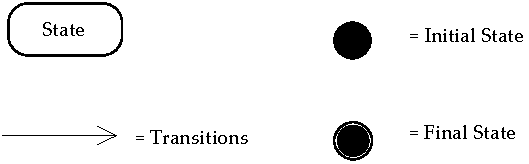
\includegraphics[width=3.28in,height=1in]{./image1}
\caption{Symbols used in state diagrams.}
\label{figure:stateDiagramSymbols}
\end{figure}


As an example, consider a vending machine that accepts nickels and dimes
and dispenses a piece of candy when 25 cents has been deposited. This
vending machine can be modeled using a state diagram because the
response of the machine to a coin depends on how much money has been
deposited so far.

In order to give a more complete description of the vending machine the
state diagram is embedded into the function table template introduce in
Chapter 5as shown in Figure~\ref{table:stateVendingMachine}.
 This table lists the inputs and outputs
of the vending machine along with the behavior represented by a state
diagram.

\begin{table}
\caption{A state diagram for a simple vending machine.}
\label{table:stateVendingMachine}
\begin{tabular}{|l|m{10cm}|}
\hline
\emph{Module} &Vending Machine Control Unit \\ \hline
\emph{Inputs} & 
\begin{itemize}
\item
  Nickel: Signals that a nickel has been deposited.
\item
  Dime: Signals that a dime has been deposited.
\end{itemize} \\ \hline

\emph{Outputs} & 
\begin{itemize}
\item
  Reset: Signals the FSM to return to the Initial/Reset state.
\item
  Vend: Signal to dispense candy.
\end{itemize} \\ \hline
\emph{Functionality} &
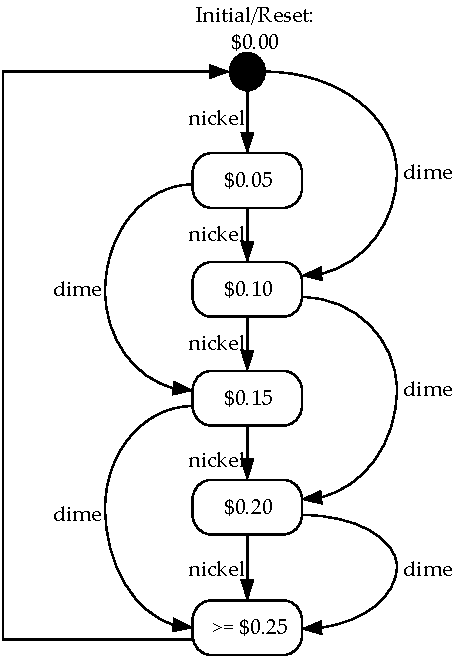
\includegraphics[width=2in,height=3in]{./image2} \\ \hline
\end{tabular}
\end{table}


The initialization/reset state is labeled \$0.00, while the action of
the machine (dispense or not dispense candy) is associated with the
states---the only state that dispenses candy is \$0.25. There are three
types of transitions shown in this state diagram. The two labeled nickel
and dime are associated with depositing those coins. The unlabeled
transition from state \$0.25 to state \$0.00 is called an unconditional
transition. A system with an unconditional transition between two states
is assumed to remain in the first state for a defined time period before
automatically moving to the second state. In this case it ensures that
the machine dispenses a single candy before going on to the next
transaction. It is common practice in state diagrams to assume that any
unspecified input conditions cause the system to remain in the current
state. For example, if no coin is inserted while in state \$0.20 the
system remains in state \$0.20. Finally, note that since this machine
does not dispense change, it can overcharge a customer for candy. This
would not be a popular vending machine with users!

\section{Flowcharts}
\label{section:flowcharts}

The intention of a \emph{\textbf{flowchart}} is to visually describe a
process or algorithm, including its steps and control. Flowcharts are
often scoffed at as being old-fashioned and overly simple---these
criticisms are actually strengths. Since flowcharts have been around for
a long time, they are easily recognized and understood. Furthermore,
being simple makes them accessible to a wide audience. Due to their
simplicity, they are applied in a great number of applications,
including non-technical ones such as the description of business
processes.

Some of the primary symbols used in flowcharts are shown in 
Figure~\ref{figure:basicFlowChartSymbols}.
The names of the starting and ending steps of a flowchart are
represented by ovals known as terminators. Individual processing steps
are written inside of rectangles, while a process step that is
elaborated by another flowchart is drawn as a rectangle with double
sides. Elaborated processes allow the representation of hierarchy in the
design. Certain points in a flowchart can lead to alternative
destinations as represented by a decision or conditional symbol
(diamond). The condition that determines the next step is written inside
the diamond and the possible values of the condition are written on the
arcs leaving the conditional step. As shown in 
Figure~\ref{figure:basicFlowChartSymbols} there are
multiple ways to indicate data stores for retrieving or saving data.

\begin{figure}
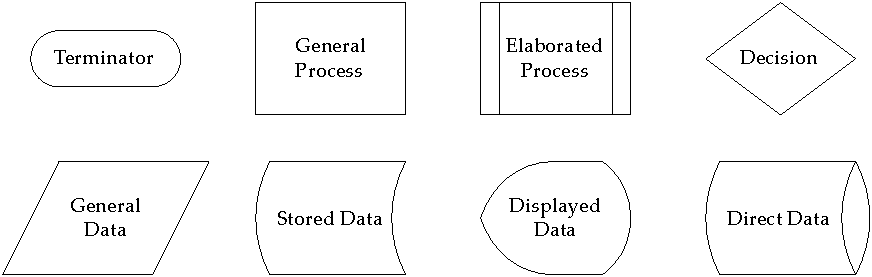
\includegraphics[width=4.9in,height=1.56in]{./image3}
\caption{Basic flowchart symbols.}
\label{figure:basicFlowChartSymbols}
\end{figure}

As an application, consider an embedded computer system that monitors
the light level of its environment as described by the flowchart in
Figure~\ref{table:flowchartEmbedded}. 
The algorithmic process of the flowchart is easy and
intuitive to understand. The system reads the current light value,
stores it into an array, and then computes an average. In a complete
system description, there would be a second flowchart describing how the
system determines the average of the values of the light samples, since
this is identified as an elaborated process. The system then waits 1ms,
writes the average to a terminal (display device), and then checks for a
key-press. Light levels continue to be monitored in the absence of a
key-press, otherwise the light monitoring process halts.


\begin{table}
\caption{A flowchart for an embedded system.}
\label{table:flowchartEmbedded}
\begin{tabular}{|l|m{10cm}|}
\hline

\emph{Module} & Light level data logger \\ \hline
\emph{Inputs} & 
\begin{itemize}
\item
  Light intensity: Ambient light intensity from environment.
\item
  Key-press: User request to abort data logging.
\end{itemize}\\ \hline

\emph{Outputs} & 
\begin{itemize}
\item
  Terminal: Displays the average light intensity.
\item
  Disk: Stores a record of light intensities through time.
\end{itemize} \\ \hline
\emph{Functionality} &
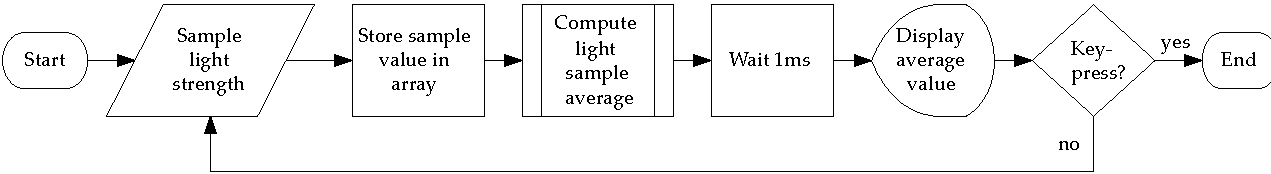
\includegraphics[width=4.7in,height=0.74in]{./image4} \\ \hline
\end{tabular}
\end{table}

\textbf{Figure 6.4} 

Flowcharts are an intuitive way to describe algorithmic processes.
Limiting the complexity of a flowchart to between 10 and 20 steps
enables the sequence of actions to be quickly comprehended while
eliminating unnecessary details. Flowcharts are not able to represent
the structure of data being manipulated and they are not particularly
good at representing concurrent processes. For this we need data flow
diagrams.

\section{Data Flow Diagrams}
\label{section:data-flow-diagrams}

The intention of a \emph{\textbf{data flow diagram}} (DFD) is to model
the processing and flow of data inside a system. It is a
function-oriented approach that is similar to functional
decomposition---the processes inside a DFD accept data inputs, transform
them in some way, and produce output data. A DFD is often used for the
analysis of information systems due to its data emphasis, but can be
broadly applied to ECE systems. It differs from functional decomposition
in that functional decomposition is often closer to the implementation
of the design, whereas the DFD models the system from a data point of
view. A DFD is fundamentally different from a flowchart in that it does
not encapsulate control and sequencing information, but allows multiple
processes running concurrently. There are four symbols, shown in 
Figure~\ref{figure:dataFlowSymbols}, that are used in a DFD:

\begin{enumerate}
\def\labelenumi{\arabic{enumi}.}
\item
  \emph{Processes.} A rectangle with rounded corners that describes a
  useful task or function. They perform a transformation on the data.
\item
  \emph{Data flows.} An arrow representing a data relationship between
  two processes.
\item
  \emph{Data stores.} An open rectangle representing a data repository.
\item
  \emph{Interfaces.} A square describing external agents or entities
  that use the system. They are also referred to as sources and sinks.
\end{enumerate}


\begin{figure}
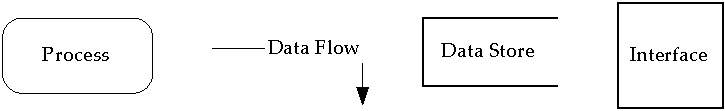
\includegraphics[width=4.6in,height=0.71in]{./image5}
\caption{Data flow diagram symbols.}
\label{figure:dataFlowSymbols}
\end{figure}


Like the general design process, DFDs are successively refined from the
top-down. That is, there is a single top level (or Level 0) DFD
describing the entire system and the interfaces and data stores that it
interacts with. The rules for constructing a DFD are fairly intuitive. A
process must have at least one input and one output. The refinement of a
process at level N must have the same inputs and outputs as the process
at level N-1. Data must be transformed in some way by a process. This
process of refinement continues until a satisfactory level of detail is
reached.

An example of a Level 1 DFD for a video browsing system is shown in
Figure~\ref{table:dataflowVideoBrowse}. Video databases are typically 
very large; due to their size,
it is usually cumbersome to preview videos and extract important
information. A solution to this problem is to apply image analysis
techniques to identify shots (continuous scenes without a break) in a
video and store both the location of the shot boundaries in the video
and key frames that summarize each shot. The collection of key frames is
known as a storyboard. The storyboards are stored in an annotation
database that is much smaller in size than the original video database.
Typically the user of a video browsing system has the ability to preview
the storyboard and select shots from it to view. This example shows the
data flow for such a system.

The data processing is readily apparent from the DFD. Videos in the
database are processed to extract shot boundaries and key frames, which
are stored in the annotation database. The user can submit requests to
view a storyboard, which is retrieved from the annotation database. When
a shot is selected from the storyboard, the users can preview the
original shot, which is retrieved from the video database.

\begin{table}
\caption{Level 1 data flow diagram for a video browsing system.}
\label{table:dataflowVideoBrowse}
\begin{tabular}{|l|m{10cm}|}
\hline
\emph{Module} & Video Browsing System \\ \hline

\emph{Inputs} & 
\begin{itemize}
\item
  Video: External video to the system that is entered into the video
  database.
\item
  Browse Request: User request to browse a particular video.
\item
  Shot Preview Request: User request to preview a particular short from
  a video.
\end{itemize}  \\ \hline
\emph{Outputs} & 
\begin{itemize}
\item
  Story Board: A sequence of frames summarizing the entire video.
\item
  Shot: The complete video corresponding to the still image in the story
  board.
\end{itemize}\\ \hline
\emph{Functionality} &

\includegraphics[width=4.9in,height=3.15in]{./image6} \\
\end{tabular}
\end{table}

There are a few important points to note about DFDs. They are solution
independent, specifying the behavior based upon data flow. Specific
information on the data flows is defined in a formal language known as a
\emph{\textbf{data dictionary}} (it is not covered here). There can be
concurrent processes represented in a DFD. In the video browsing
example, multiple people can use the system simultaneously, and there is
no implied sequencing between when the shot boundary detection process
is run and the storyboards are previewed. It is clear that the video
must undergo shot detection prior to viewing its storyboard. This
information is listed in something known as an \emph{\textbf{event
table}}. The event table for this example is shown in Table 6.1.

\textbf{Table 6.1} Event table for the video browsing system.

\begin{table}
\caption{}
\label{table:<context>}
\begin{tabular}{|c|c|c|c|}
\hline
\textbf{Event} & \textbf{Trigger}& \textbf{Process} & \textbf{Source} \\ \hline
Annotate Video & New Video Arrival & Shot Boundary Detection & System \\  \hline
View Storyboard & Browse Request & Storyboard Preview & User \\ \hline
View Shot & Shot Preview Request & Shot Preview & User \\ \hline
\end{tabular}
\end{table}

An \emph{\textbf{event}} is an occurrence at a specific time and place
that needs to be remembered. Events can be classified into temporal,
external, and state. A \emph{temporal event} is one which happens
because the system has reached some critical time. In this example, the
generation of shot boundaries could occur for all new videos in the
database at a specified time each day, but in this case it occurs
whenever a new video is added to the database. An \emph{external event}
occurs outside the system boundary by a system user, in this case
requesting either a storyboard or a video preview. A \emph{state event}
is the result of something changing within the system. Associated with
each event is a \emph{trigger}, the cause of the event. Each event has a
process that is associated with it. Finally, associated with each event
is a \emph{source}, the entity responsible for triggering it.

\section{Entity Relationship Diagrams}
\label{section:entity-relationship-diagrams}

A database is a system that stores and retrieves data, and it is modeled
by an \emph{\textbf{entity relationship diagram}} (ERD). The intention
of an ERD is to catalog a set of related objects (entities), their
attributes, and the relationships between them. The entities and their
relationships are real distinct things that have characteristics that
need to be captured. The design of a database starts by describing the
entities, their attributes, and the relationship between entities in an
ERD. In order to ask meaningful questions about the data, the entities
need to be related to one another. For example, a list of students and a
list of courses by themselves have limited utility. However, by
introducing a relationship between these two entities we can ask
questions such as ``\emph{How many students are taking the
Microelectronics course?}'' The three elements used in the ERD modeling
language are:

\begin{enumerate}
\def\labelenumi{\arabic{enumi}.}
\item
  \emph{Entities.} They are generally in the form of tangible objects,
  roles played, organizational units, devices, and locations. An
  instance is the manifestation of a particular entity. For example, an
  entity could be Student while an instance would be Kristen.
\item
  \emph{Relationships.} They are descriptors for the relationships
  between entities.
\item
  \emph{Attributes.} They are features that are used to differentiate
  between instances of the entities.
\end{enumerate}

Lets consider an ERDs describing academic life at a college . The
process typically starts by interviewing the end-users and identifying
the entities and their attributes. Assume that the result of this
process is that the college wants to store data about three entities:
Students, Courses, and Departments. The process of building an ERD
starts by determining the relationships between entities. One way to do
this is to build an \emph{\textbf{entity relationship matrix}} as shown
in Table~\ref{table:entityRelationshipMatrix}. 
The entities constitute both the row and column headings,
and the matrix entries represent the relationship, if any, that exists
between entities. This is similar to the pairwise comparison matrix in
Chapter 2 where user needs were systematically compared. Relationships
are bi-directional because they have two participating entities.

\begin{table}
\caption{Entity relationship matrix.}
\label{table:entityRelationshipMatrix}
\begin{tabular}{|c|c|c|c|}
\hline
\textbf{Student} & \textbf{Course} & \textbf{Department} \\ \hline
\textbf{Student} & & takes many & majors in one \\ \hline
\textbf{Course} & has many & can require many / can be the prerequisite
for many & is offered by one \\ \hline
\textbf{Department} & enrolls many & offers many & \\ \hline
\end{tabular}
\end{table}

From Table~\ref{table:entityRelationshipMatrix} we can 
see that a Student can take many courses and a
Course has many students in the Student-Course relationship. A
\emph{\textbf{cardinality ratio}}, associated with each relationship,
describes the multiplicity of the entities in a relationship. For
example, the Student-Course relationship is many-to-many, or M:M,
because one student can take \ul{many} courses and one course is taken
by \ul{many} students. The relationship between Student and Department
is M:1 since a Department enrolls \ul{many} students, but a student can
major in only \ul{one} Department. A recursive relationship,
prerequisite, exists between the Course entity and itself because a
course may have \ul{many} other courses as prerequisites and may be the
prerequisite for \ul{many} other courses. Thus the prerequisite
relationship has an M:M cardinality. It needs to be noted that in this
example the needs of the college required relationships between all
pairs of entities. If, for example, the college did not need to keep
track of the students' majors, then the relationship between Student and
Department would be left blank in the entity relationship matrix.

The resulting ERD is shown in Figure~\ref{table:erdCollegeSystem}. 
The relationships are
identified by the diamonds shaped symbols; the entities are denoted by
the rectangles with their name at the top. The cardinality ratio is
labeled on the links between the relationships and entities. Another
piece of information shown in the ERD is the attributes associated with
each entity. An attribute is a feature or characteristic of an entity
that needs to be remembered. There are many different types of
attributes; however, the most important are \textbf{\emph{key
attributes}} (which are underlined) which uniquely identify instances.
For example, the identification number (ID) attribute of a Student is a
key attribute.


\begin{table}
\caption{ERD for the college database system.}
\label{table:erdCollegeSystem}
\begin{tabular}{|l|m{10cm}|}
\hline
\emph{Module} & Grade Database \\ \hline

\emph{Inputs} & 
\begin{itemize}
\item
  Students: Data about students.
\item
  Departments: Data about departments.
\item
  Courses: Data about courses.
\end{itemize} \\ \hline
\emph{Outputs} & 
\begin{itemize}
\item
  Relationship between departments and their enrolled students.
\item
  Relationship between students and the courses that they take.
\item
  Relationship between departments and the courses they offer.
\item
  Relationship between course and their prerequisite courses.
\end{itemize} \\ \hline
\emph{Functionality} &
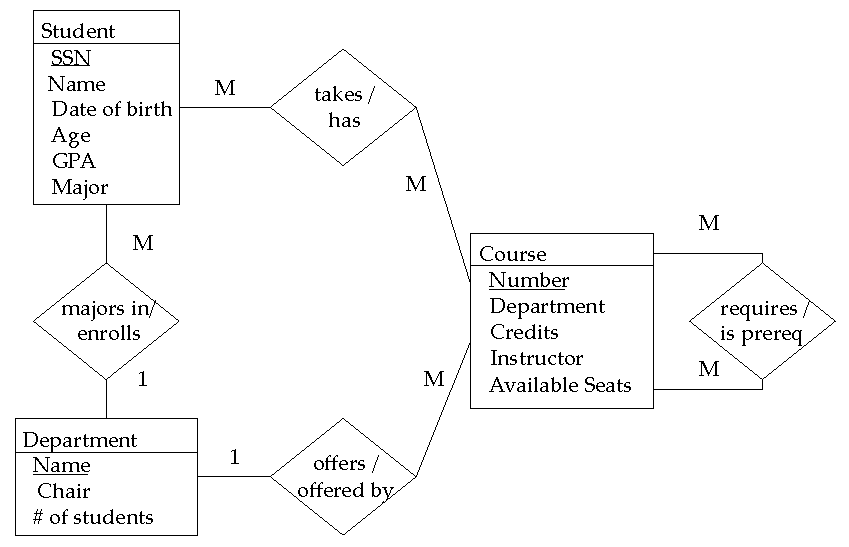
\includegraphics[width=4.5in,height=3.1in]{./image7} \\
\end{tabular}
\end{table}

The ERD allows for an easy interpretation of the relationships between
entities as well as their attributes. Although beyond the scope of the
discussion here, the ERD is a formal language that can be used to
automatically generate the database structure. The relationships in the
ERD allow queries to be asked of the resulting database. For example,
the college could derive a student's course schedule from the database
from the relationship between Student and Course.

\section{The Unified Modeling Language}
\label{section:the-unified-modeling-language}

The \emph{\textbf{Unified Modeling Language}} (UML) was created to
capture the best practices of the object-oriented software development
process. However, it has valuable modeling tools that can be applied
more generally to ECE systems. The objective of this section is to
provide an overview of UML and the six different system views that it
encompasses. A caveat for the reader---UML is complex, and complete
coverage is beyond the scope of this book. In order to fully understand
its subtleties and nuances, the reader is advised to consult the
references provided in Section 6.8.

In order to aid in the explanation of the different views we will create
a UML model of a system called the Virtual Grocer, or v-Grocer for
short. The v-Grocer enables a user to order groceries from home and have
them delivered. The concept is to provide users with a barcode scanner
that is connected to their home computer along with application
software. When the user runs out of an item, he/she scans in the
Universal Product Code (UPC). When users want to order groceries, they
connect to the Internet, log into the grocery store web server, enter
the quantity for the scanned items, and place their order. Once the
order is completed, they are billed and the groceries are delivered to
their houses at a prearranged time.

\subsection{Static View}
\label{subsection:static-view}

Object-oriented design (OOD) is fundamentally different from functional
software design in that it emphasizes objects instead of functions.
\emph{\textbf{Objects}} represent both data (attributes) and the methods
(functions) that can act upon the data. An object represents a
particular instance of something known as a \emph{\textbf{class}}, which
defines the attributes and methods. An object encapsulates all of this
information. The data and methods that an object encapsulates are
available only to that object by default. Thus, other objects cannot
change that state of an object unless given specific permission to do
so. This improves the reliability and maintainability of software
systems, because changes made to the internal representation of a class
are not seen by methods outside of the class.

The intention of the \emph{\textbf{static view}} is to show the classes
in a system and their relationships. The static view is characterized by
a \emph{class diagram}. A very simple class diagram with a single class
is shown in Figure~\ref{figure:classDiagram}. 
The specification of a class has three parts, a
name, a list of attributes, and a set of methods. The name of the class
for this example is Customer and it has three attributes: Name, Address,
and CustId. It has one method associated with it, ChangeAddr(), which
can change the Address attribute. A class, just like an entity in an
ERD, is a generalization of a set of a particular thing or instance. For
example, the Customer class could have a particular instance called Ms.
Robinson.

\begin{figure}
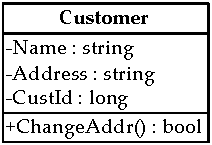
\includegraphics[width=1.2in,height=0.81in]{./image8}
\caption{Class diagram notation. The class has a label
(Customer), attributes (Name, Address, and CustId), and methods
(ChangeAddr()).}
\label{figure:classDiagram}
\end{figure}

Classes are related to one another by relationships that define how
classes interact with each other. For example, if a class is a subset of
another class (a kind of relation) then the subclass inherits all the
attributes and methods of the \emph{superclass}. In UML, there are a
host of relationships; among these are generalization, composition, and
associations. Two classes are related by a \emph{generalization
relationship} when one is a subset of the other. Two classes are related
by a \emph{composition relationship} when one is composed of members of
the other. Two classes are related by an \emph{association relationship}
whenever they need to send messages to one another. Relationships are
drawn as lines connecting the two participant classes. The terminals of
the line have different shapes depending on the type of relationship.
Just like an ERD, the relationships between classes have cardinality
defined by the rule base. In order to illustrate these points, 
Figure~\ref{figure:classVgrocer} 
shows the class diagram for a portion of the v-Grocer system.

\begin{figure}

\includegraphics[width=3.56in,height=2.6in]{./image9}
\caption{Class diagram for the v-Grocer.}
\label{figure:classVgrocer}
\end{figure}

The class diagram has five classes---Customer, Delivery, Order, Item,
and GroceryCart. The GroceryCart class is derived from the many-to-many
relationship which exists between the Order and Item classes. Just like
the rules for an ERD, the cardinality of a relationship is read at the
end of the association in which it is involved. The only difference is
that the many cardinality in a class diagram is denoted by a * symbol.
For example, a delivery is sent to one customer, while a customer may
receive many deliveries.

\subsection{Use-Case View}
\label{subsection:use-case-view}

The intention of the \emph{\textbf{use-case view}} is to capture the
overall behavior of the system from the user's point of view and to
describe cases in which the system will be used. It is characterized by
a \emph{use-case diagram}, and an example for the v-Grocer is shown in
Figure~\ref{figure:useCaseVgrocer}. 
There are only two symbols employed in a use-case diagram,
actors and use-cases. Actors, drawn as stick figure people, are
idealized people or systems that interact with the system. For this
example the actors are customers, delivery people, the database, clerks,
and the web server. Use-cases are drawn as ovals in the diagram, and in
this example, they are WebOrder, DeliverOrder, and AssembleOrder. A
use-case is a particular situation when actors use the system and is
usually represented by a sequence of actions that will be performed by
the system. This sequence of actions typically represents a high level
of functionality. Every actor that interacts with a particular use-case
is connected to it with a line. Finally, the entire collection of
use-cases is enclosed in a rectangle with the actors outside. This
rectangle represents the system boundary and consequently is labeled
with the name of the system.

\begin{figure}
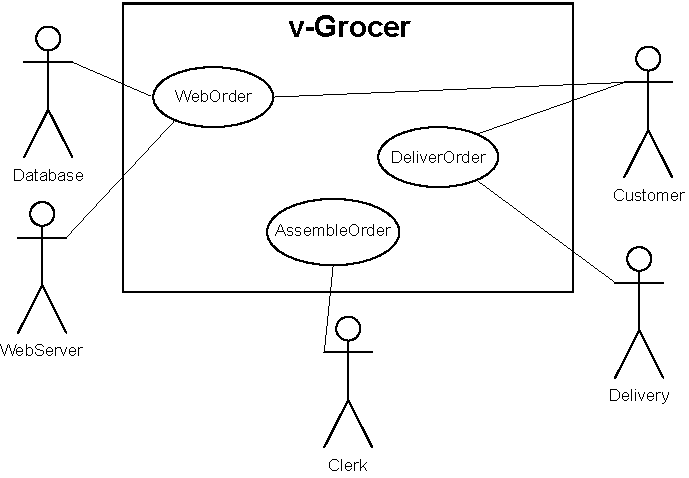
\includegraphics[width=3.9in,height=2.7in]{./image10}
\caption{Use-case diagram for the v-Grocer.}
\label{figure:useCaseVgrocer}
\end{figure}

From Figure~\ref{figure:useCaseVgrocer}
it is apparent that a Customer, the WebServer, and
Database interact when creating a WebOrder. Use-cases are often
described in a table as shown for this particular example in 
Table~\ref{table:webOrderUseCase}.

\textbf{Table 6.3} 


\begin{table}
\caption{WebOrder use-case description.}
\label{table:webOrderUseCase}
\begin{tabular}{|l|m{10cm}|}
\hline
\textbf{Use-Case} & WebOrder \\ \hline
\textbf{Actors} & Customer, Database, and WebServer \\ \hline
\textbf{Description} & This use-case occurs when a customer submits an
order via the WebServer. If it is a new customer, the WebServer prompts
them to establish an account and their customer information is stored in
the Database as a new entry. If they are an existing customer, they have
the opportunity to update their personal information. \\ \hline
\textbf{Stimulus} & Customer order via the GroceryCart. \\ \hline
\textbf{Response} & Verify payment, availability of order items, and if
successful trigger the AssembleOrder use-case. \\ \hline
\end{tabular}
\end{table}

Use-cases focus on a very high level of functionality and describe who
will interact with the system and how they will interact. Given their
high level of abstraction, they can easily be incorporated into a
variety of ECE projects. They are also simple and easy to understand and
thus can be incorporated into presentations to non-technical audiences.
Finally, use-cases are simply not busy work---they are fundamental to
the development of other UML models.

\subsection{State Machine View}
\label{subsection:state-machine-view}

The \emph{\textbf{state machine}} \emph{\textbf{view}} is characterized
by a \emph{state diagram} as was discussed in Section 6.2. Again, the
intention of a state diagram is to describe systems with memory. 
Figure~\ref{figure:stateDiagramVgrocer} shows the state 
view of a customer logging into the v-Grocer web
server.


\begin{figure}
\includegraphics[width=2in,height=2.in]{./image11}
\caption{State diagram for the v-Grocer customer login.}
\label{figure:stateDiagramVgrocer}
\end{figure}

\subsection{Activity View}
\label{subsection:activity-view}

The intention of the \emph{\textbf{activity view}}, characterized by an
\emph{activity diagram}, is to describe the sequencing of processes
required to complete a task. In UML, the tasks elaborated are the
individual use-cases identified in a use-case diagram. Since more than
one actor may be involved in completing a task, an activity diagram can
express the concurrent nature of tasks. An activity diagram is composed
of states, transitions, forks, and joins. 
Figure~\ref{figure:activityDiagramVgrocer} contains an
activity diagram for the v-Grocer order delivery system. The diagram
gives a clear visual picture for the activities that need to be
completed for an order to be packed and delivered. After a complete
order is placed, the flow is forked into two concurrent processing
branches. One of these branches is for completion of the order, while
the other addresses its scheduling, delivery, and coordination with
other deliveries. When both of those processes are completed, they are
joined together and then the delivery run is made.


\begin{figure}
\includegraphics[width=5.5in,height=0.9in]{./image12}
\caption{Activity diagram for order processing and delivery
for the v-Grocer.}
\label{figure:activityDiagramVgrocer}
\end{figure}

\subsection{Interaction View}
\label{subsection:interaction-view}

The intention of the \emph{\textbf{interaction view}} is to show the
interaction between objects. It is characterized by collaboration and
sequence diagrams. In an object-oriented system, tasks are completed by
passing messages between objects. The interaction view shows how
messages are exchanged in order to accomplish a task. These tasks are
usually the use-cases. Since messages are sent through time, the
interaction view must be able to express the concept of order. We start
by examining collaboration diagrams.

Two objects collaborate together in order to produce some meaningful
result. A \emph{collaboration diagram} shows the sequencing of messages
that are exchanged between classes in order to complete a task. It
consists of the classes that participate in the realization of the task
and the messages exchanged. The messages are drawn as arrows from the
sending object to the receiving object. The message arrows are labeled
with the name of the message and its numerical position in the sequence
of messages exchanged to realize the task. For example, 
Figure~\ref{figure:collaborationDiagramWebOrder}
shows how the WebOrder use-case is realized using the Customer,
WebServer, and Database classes. Note, WebServer and Database are
introduced as new classes and are not shown as part of the class diagram
in Figure 6.9.

\begin{figure}
\includegraphics[width=4in,height=1.17in]{./image13}
\caption{Collaboration diagram for the WebOrder use-case.}
\label{figure:collaborationDiagramWebOrder}
\end{figure}


The collaboration diagram is similar in form to the class diagram, the
difference being that the relationships are annotated with the messages
that are exchanged. Consequently, the collaboration diagram aides the
developers in understanding and implementing the methods used between
classes. In order to emphasize the order in which messages are
exchanged, a developer can also use a sequence diagram.

A \emph{sequence diagram} contains the same information as the
corresponding collaboration diagram. Where the collaboration diagram
emphasizes the objects that interact to produce a behavior, a sequence
diagram emphasizes the message order that produces a behavior. As shown
in Figure~\ref{figure:sequenceDiagramWebOrder}, 
the classes that participate in the behavior are listed
in a row at the top of the diagram. From each class a dotted vertical
line is drawn downward that represents the lifeline of its class (the
vertical axis represents time). When an object is actively requesting or
waiting for information from another object, a rectangle is drawn over
the dotted lifeline of the object. The message is drawn as an arrow from
the sending object to the receiving object and labeled with the name of
the message. The activity diagrams can be applied generally to ECE
systems to show the interaction between entities, particularly the
sequencing of messages.

\begin{figure}
\includegraphics[width=2.6in,height=2.4in]{./image14}
\caption{Sequence diagram for the WebOrder use-case.}
\label{figure:sequenceDiagramWebOrder}
\end{figure}

\subsection{Physical View}
\label{subsection:physical-view}

The intention of the \emph{\textbf{physical view}} is to demonstrate the
physical components of the system and how the logical views map to them.
The physical view is characterized by a component and deployment
diagram. A \emph{component diagram} shows the software files and the
interrelationships that make up the system. Software files are shown in
rectangles. Lines connect together files that need to communicate. A
\emph{deployment diagram} shows the hardware and communications
components that will be used to realize the system. The hardware
components are drawn as cubes and labeled with their names. 
Figure~\ref{figure:vGrocerSystem}
shows a combined component and deployment diagram for the v-Grocer
system. The software files are the Browser, v-Grocer, Apache, and
Oracle, while the hardware components are the Customer, WebServer, and
Database.

\begin{figure}
\includegraphics[width=4.8in,height=1.4in]{./image15}
\caption{The combined component and deployment diagram for
the v-Grocer. The software files are the Browser, v-Grocer, Apache, and
Oracle, while the hardware components are the Customer, WebServer, and
Database.}
\label{figure:vGrocerSystem}
\end{figure}


\section{Project Application: Selecting Models}
\label{section:project-application-selecting-models}

Chapters 5 and 6 have presented a variety of models for representing the
behavior of systems. The design team needs to select the correct
combination of tools to properly describe a design for its eventual
implementation. Table 6.4 provides a summary of the models and their
different intentions.

Table 6.4

\begin{table}
\caption{Guidance for model selection.}
\label{table:<context>}
\begin{tabular}{|l|m{10cm}|}
\hline
\textbf{Model} & \textbf{Intention} \\ \hline
\textbf{Functional Decomposition} & To describe the input, output, and
functional transformations applied to information (electrical signals,
bits, energy, etc.) in a system. It is broad in application. This often
provides a view that is close to the actual system implementation. See
Chapter 5. \\ \hline
\textbf{State Diagram} & To describe the behavior of systems with
memory. They are very flexible when it comes to application. They are
often applied to digital design, but state diagrams can also be used to
describe the high level behavior of complex systems. The only
prerequisite on their use is that the system has memory. See Section
6.2. \\ \hline
\textbf{Flowchart} & To describe a process or algorithm, including its
steps and control. They are applicable to many problem domains from
software to describing business practices. See Section 6.3. \\ \hline
\textbf{Data Flow Diagram} & To model the processing, transformation, and flow of
data inside a system. They are typically supplemented by an event table
describing all possible events and the resulting actions. Creating a DFD
requires the designer to carefully think about the uses of the system
and how the system is to react to external users and events. See Section
6.4. \\  \hline
\textbf{Entity Relationship Diagram} & To catalog a set of related objects (entities), their
attributes, and the relationships between them. ERDs capture the
entities and relationships of a portion of the world into a formal data
model. The graphical language describes the attributes of the entities
and the cardinality of the relationships. ERDs are formal enough to be
unambiguously translated into a complete description of a database
system. See Section 6.5. \\  \hline
\textbf{The Unified Modeling Language.} & The intention of UML is to
describe complex software systems. However, certain views are well
suited to describing systems at a high level and are applicable to many
domains. The process of viewing a system from the six perspectives
listed below decreases the chances that crucial details of the design
will be overlooked. \\  \hline
\textbf{Class Diagram} & To describe classes and their relationship in
an object-oriented software system. Class diagrams are primarily for
software design and are not easily accessible to a non-technical
audience. See Section 6.6.1. \\ \hline
\textbf{Use-Case Diagram} &  To capture the overall behavior of the system from
the user's point of view and describe cases in which the system will be
used. See Section 6.6.2. \\  \hline
\textbf{State Machine} & This is essentially the same as the state
diagram, but is also a formal UML view. See Sections 6.2 and 6.6.3. \\  \hline
\textbf{Activity Diagram} &  To describe the sequencing of processes required to
complete a task. Composed of states, transitions, forks, and joins. Can
show concurrent processes. See Section 6.6.4. \\  \hline
\textbf{Interaction Diagram} & To show the interaction and passing of messages
between entities in a system. Characterized by both collaboration and
sequence diagrams. See Section 6.6.5. \\  \hline
\textbf{Physical Diagram} &  To describe the arrangement and connections of the
physical components that constitute a system. In the case of UML, it is
characterized by a component and deployment diagram. See Section
6.6.6. \\  \hline
\end{tabular}
\end{table}

\section{Summary and Further Reading}
\label{section:summary-and-further-reading}

Models provide a convenient method of describing a system at a high
level of abstraction. This allows a system to be described without
having to determine all of the implementation details. All models are
not the same---they come in a variety of forms and each is designed to
serve a different intention. The properties of effective models were
presented, and we saw that they are similar to those of an engineering
requirement. Models should encourage innovation by allowing the
exploration of alternative implementations. Since models are built from
abstractions of the actual system components, they are an effective
means for communicating with non-technical stakeholders. Finally, models
provide an excellent means of documenting the development of a design
from the highest level down to the detailed design.

This chapter presented a variety of models for describing system
behavior that included state diagrams, flowcharts, data flow diagrams,
entity relationship diagrams, and the Unified Modeling Language. Table
6.4 provides a quick reference that describes the intention and
application of the models examined in both Chapters 5 and 6.

Flowcharts have been around for quite some time and an early work
describing them is \ul{Flowcharts} by Chapin {[}Cha71{]}. The book
\ul{Programming Logic and Design} {[}Far02{]} covers flowcharts
extensively and their application in programming. State diagrams are
fundamental to the ECE field and further information on them is
available in virtually any introductory digital design textbook. Data
flow diagrams and entity relationship diagrams are common tools used in
information systems analysis and design and can be further explored in
\ul{Systems Analysis and Design} {[}Sat02{]} and \ul{Fundamentals of
Database Systems} {[}Elm94{]}. Two references for UML are \ul{The
Unified Modeling Language Reference Manual} {[}Rum98{]} and \ul{Schaum's
Outline of UML} {[}Ben01{]}.

%\section{Problems}
\label{section:behavModelsProblems}

\begin{enumerate}
\def\labelenumi{\arabic{enumi}.}
\item
  Why is it important for a model to separate the design of a system
  from its realization?

\item
  Classify each of the following as either a model, not a model, or
  sometimes a model. Justify your answer based on the definition and
  properties of a model.

\begin{itemize}
\def\labelenumi{\alph{enumi})}
\item A diagram of a subway system,
\item a computer program, 
\item a football play, 
\item drivers license,
\item a floor plan of the local shopping mall (a ``you are here'' diagram)., 
\item an equation, 
\item A scratch n' sniff perfume advertisement in a fashion magazine,
\item The 1812 overture,
\item a braille sign reading ``second floor'',
\item sheet music for the Brandenburg Concerto, 
\item the United States Constitution, 
\item a set of car keys,
\item the ASCII encoding of an email message.
\end{itemize}


  \item
    Which of the following systems has memory? Justify your answer using
    the concepts of input, output, and state.
\begin{itemize}
\def\labelenumi{\alph{enumi})}
\item  an ink pen,
\item a resistor,
\item a capacitor,
\item a motorized garage door,
 \item an analog wrist watch, 
\item the air pressure in an air compressor, 
\item  the thermostat which controls the furnace in a house, 
\item a light switch, 
\item a political system,
\item the temperature of a large lake, 
\item  a book, 
\item a computer's hard drive.
\end{itemize}


  \item
    A can of soda has memory. Your objective is to figure out what
    characteristic of the can is the state variable and what input
    causes it to change. Based upon this, draw a state diagram for a can
    of soda. Label the transition arcs with the input responsible for
    the transition. Hint: no special equipment is needed to elicit the
    change of state.
  \item
    Consider the state diagram for the vending machine shown in 
    Table~\ref{table:stateVendingMachine}.
    Now assume that the system accepts nickels, dimes, and
    quarters. Also assume that it is capable of returning change to the
    user after a purchase. Create a state diagram that represents this
    new system. Make sure to define the output signals and their value
    for each state.
  \item
    Use a state diagram to describe the high level operation of the
    ChipMunk Recorder (CMR). The CMR records sounds and then plays them
    back at a variety of speeds, making a recorded voice sound like a
    high pitched chipmunk. The CMR receives user input from a keyboard
    and an audio source. The behavior of the system is described as
    follows:

\begin{itemize}
\item
  When powered up, the CMR enters a wait state.
\item
  If \textquotesingle R\textquotesingle{} is pressed the recorder begins
  recording.
\item
  Any key-press will put the CMR back into the wait state.
\item
  If \textquotesingle S\textquotesingle{} is pressed, the CMR is ready
  to change the playback speed. A subsequent numerical input between 1
  and 5 will cause the playback speed to be changed to that value.
\item
  Pressing the \textquotesingle R\textquotesingle{} key when in the
  adjust playback speed mode will cause the CMR to go to the wait state.
\item
  Pressing a \textquotesingle P\textquotesingle{} key will cause the CMR
  to playback the recorded sounds. When done playing the entire
  recording, the CMR will loop back and start playing at the beginning.
\item
  Any key-press while in the playback mode will cause the CMR to go back
  into the wait state.
\end{itemize}

  Draw a state diagram describing the behavior of the CMR. Create a
  table which lists every state and its associated output.

  \item
  \label{problem:stateDiagramTapeCartridges}
    Build a state diagram to describe the state of the tape cartridges
    used to backup a company's network drives. When new
    \textbf{unformatted} cartridges are received they are immediately
    labeled with a unique ID. Before a tape is used it is formatted
    turning it into a \textbf{blank} tape. On the first day of the week
    a complete backup is made of the network drives, transforming blank
    tapes into \textbf{active} tapes. The active tapes, made every
    fourth week, are moved off site making them \textbf{archival} tapes.
    Active tapes older than 3 months are assumed to have out of date
    information and are reformatted into blank tapes. Archival tapes
    more than 2 years old are reformatted and put back into circulation.
  \item
    Build a flowchart to describe the operation of a microcontroller
    (MCU) based temperature regulating system. The system monitors the
    temperature of a heated environment using thermistors and regulates
    the temperature by turning fans on to cool the environment. The MCU
    periodically reads the temperature from each of the 64 different
    thermistors (each is driven by its own constant current source) by
    selecting each through an analog multiplexor. The voltage is
    converted into an 8-bit digital value using the MCU's
    analog-to-digital converter. If any of the 64 thermistors exceeds a
    high temperature threshold, the MCU uses a complex algorithm to
    determine the number of fans to turn on, otherwise all the fans are
    turned off.
  \item
    Write an algorithmic description for each of the flow charts below
    using while, if, or do statements.

\begin{tabular}{m{4cm}m{4cm}m{4cm}}
\includegraphics[width=1.26in,height=1.08in]{./image16} &
\includegraphics[width=0.747in,height=1.35in]{./image17} &
\includegraphics[width=2.16in,height=1.314in]{./image18} \\
(a) &  (b)  & (c) \\
\end{tabular}

\item
  Create a flowchart that outlines how to crochet a two-tone blanket
  with a diagonal stripe across it as shown below. A blanket is
  crocheted by linking together a sequence of basic stitches. For the
  purposes of the flowchart assume that a basic stitch is an elaborate
  process. Basic stitches are made from either dark or light yarn. The
  blanket should be 100 stitches wide by 150 stitches high. The diagonal
  stripe runs at a 45 degree angle from the horizontal.

\includegraphics[width=1in,height=1.34in]{./image19}


\item
  Build a data flow diagram and event table to represent an image
  archiving system for an art museum. The art museum maintains a
  database of digital images of paintings from museums all over the
  world. The following information is known about the image database
  system:

\begin{itemize}
\item
  Images are shared among museums in a participating network. Whenever a
  participating museum posts a new image, it sends a broadcast email to
  all participating museums in the network with the image attached as an
  email. It provides the name of the painting and artist in the body of
  the email. All new images received are added directly to the museum's
  own image database.
\item
  When inserted into the museum's database, each image is provided with
  a tag identifying the name of the painting and the artist.
  Furthermore, this triggers an image analysis routine that classifies
  the image based into predefined categories such as portrait, natural
  scene, and modern. Furthermore, it stores key features that are
  extracted from the image.
\item
  The key features are used to identify and retrieve visually similar
  images from the museum's database. Another image processing algorithm
  is run that compares the visual similarity of the new image to all
  images in the database. This process produces a matching score of 0 to
  100 that is stored.
\item
  The museum's image database is available to visitors via computer
  kiosks placed throughout the museum. Kiosk users can retrieve and view
  images in one of three ways. First, they can specify the name of the
  artist or painting. Second, they can retrieve a class of images, such
  as modern. Third, once they have received a painting, they can submit
  a request to view visually similar images. The visually similar images
  are retrieved for viewing based upon the matching score.
\end{itemize}

  \item
    Build an ERD to keep track of the bicycle frames manufactured at a
    local company. The following are notes from an interview with the
    owner.


\begin{quote}
\emph{We custom build bike frames to the dimension of each individual
customer. When a customer comes in we take measurements in their height,
leg length, arm length, torso length, weight, and waist measurement.
Since we have high customer satisfaction our customers order new frames
every several year. Hence we would like to date these measurements in
order to track how a customer's body changes through time .Each frame is
built on one set of measurements. Clearly, we need to keep track of our
customer's contact information like name, address, phone number, and
email address. We would like to know which employee built which frame.
We would like to store basic information like name, address, phone, and
SSN for each employee. Each frame is built by one employee using a
variety of different titanium tubing. We have strict inventory control
on all of our tubing and need to keep track of its grade, lot \#, Outer
Diameter (OD), Inner Diameter (ID), and manufacturer. Tubing is uniquely
identified by its lot \#. Finally we need to keep information on the
frame. Each frame is given a unique serial number, and has a color,
type, and dimensions.}
\end{quote}


\item
  Extend Problem~\ref{problem:stateDiagramTapeCartridges}
  to create an ERD that captures data about the tape
  cartridges used in the backup system. Every Sunday night a full backup
  is made of all network drives. A full backup creates an identical copy
  of the network drives on the tape cartridges. Due to the large amount
  of information, a full backup requires many tapes. On the other nights
  of the week an incremental backup is made. An incremental backup
  stores only files modified since the last backup (either full or
  incremental). Incremental backups are much smaller than a full backup,
  and consequently many incremental backups fit on a single tape. A tape
  contains only full or incremental backup information -- the unused
  portion of the last tape used for a full backup is never used to store
  incremental backups. Your company wants to keep track of tapes, full
  backups, and incremental backups. An ID and state should be tracked
  for each tape. For full backups, the system needs to track the
  creation date and the number of tapes used. For an incremental backup
  it should track the date it was made. The relationships between the
  backup type and the tape will capture which tapes participated in
  which backup. (Hint: the state of a tape should be an attribute of the
  tape entity - unformatted, blank, etc. They are not attributes and are
  possible values for the state attribute.)

\item
  \textbf{Project Application.} Develop behavior models that are
  applicable for describing your system. 
  Table~\ref{table:guidanceModelSelection} is provided to help
  in making the determination as to which models are applicable
\end{enumerate}


\chapter{Testing}
\label{chapter:testing}
\graphicspath{ {./chapter07/Fig} }

\begin{itquote}
A stitch in time saves nine.---Anonymous
\end{itquote}


Most systems undergo testing throughout their development and before
they are delivered to the customer. Clearly, systems should be tested to
ensure that they meet the engineering requirements. In fact, one of the
desirable properties of an engineering requirement is that it be
verifiable, or in other words, testable. The philosophy of testing is
embodied in the quote above, which means that it is better to correct
errors early, rather than wait until they become much larger problems
later. As we saw in Chapter~\ref{chapter:engineeringDesignProcess}, 
the cost to correct problems increases
exponentially with the lifetime of the project. Thus, testing should be
considered throughout system development.

Testing means different things to different people. A field service
technician, assembly line worker, and designer will have their own
definitions and requirements from a test. In this chapter testing is
examined from the perspective of a systems designer intent on checking
that the system meets the engineering requirements. Along the way
fundamental testing concepts like controllability and observability are
explored. Approaches to debugging systems are provided, followed by
templates for building unit tests, integration tests, and acceptance
tests.

\section*{Learning Objectives}
\noindent\rule{\linewidth}{1pt}
By the end of this chapter, the reader should:

\begin{itemize}
\item
  Understand the concepts of black box tests, white box tests,
  observability, and controllability.
\item
  Understand the principles of debugging.
\item
  Understand when a unit test is used and how it is constructed.
\item
  Understand when an integration test is used and how it is constructed.
\item
  Understand when an acceptance test is used and how it is constructed.
\end{itemize}

\section{Testing Principles}
\label{section:testing-principles}

The design process is really a continual increase in specificity from
engineering requirements to the detailed design. We now consider the
question of how to test that the resulting system meets the design
requirements. One answer is based on a common testing model, the ``test
vee'', shown in Figure~\ref{figure:testVee}. 
This model starts with the engineering
requirements, proceeds to the implementation, and then onto testing. It
emphasizes that every level of design has a corresponding level of test.
What is not so clear from this model is that the testing process is
actually split between the two halves of the test vee. Students
typically think of testing as being exclusively confined to the right
half of the test vee -- build it then you test it. However, each test
performed in the right half of the test vee must be carefully engineered
during the development of the system in the left side of the test vee.
An acceptance test plan should be written with the Requirements
Specification, integration tests defined and written during the system
design, and so forth.

\begin{figure}[h]
\centering
\includegraphics[width=2.9in,height=2.4in]{./image1}
\caption{The Test Vee. Design stages are on the left and
corresponding tests are on the right.}
\label{figure:testVee}
\end{figure}

In our enthusiasm to complete a project many of us all too often rely on
a ``smoke test'' -- turn on a system to see if it works. The name of
this test is a reference to what may happen to the system if the test
fails -- it burns up and smokes. Beyond being a potentially expensive
way to test a system, a smoke test is not a systematic approach to
verify that the system behaves as expected. Customer are not be
impressed with ``hey it didn't catch on fire!'' as the test result.
Clear tests need to be developed because:

\begin{itemize}
\item
  The test cases define exactly what the module must do.
\item
  Testing prevents feature creep, since the development of a module is
  complete when its test is passed.
\item
  Test cases motivate developers by providing immediate feedback.
\item
  Test cases force designers to think about extreme cases.
\item
  Test cases are a form of documentation.
\item
  Test cases force the designer to consider the design of the module
  before building it.
\end{itemize}

The test suite and its accompanying documentation contain important
information about the behavior and organization of a system and its
module. This gives tests a value beyond a role in showing that the
system and its modules do not fail the tested conditions. The individual
test cases show others engineers how to properly interface to a module,
making that module more reusable. In addition, test documents can be
used by other individuals in the organization like technical writers,
maintenance technicians, and technical trainers.

How should testing be done? Given enough time, a system could be tested
by simply enumerating every conceivable input and observing the outputs.
While in some cases this might be possible, in general it would take an
unreasonable amount of time to perform such a test. Instead, tests are
crafted in order to maximize the likelihood of finding errors.

\subsection{Types of Testing, Observability, and Controllability}
\label{subsection:types-of-testing-observability-and-controllability}

Tests fall into two general types---black box and white box tests.
\emph{\textbf{Black box tests}} are those that are performed without any
knowledge of the systems internal organization. In a black box test, the
testing is typically conducted by changing the inputs and comparing the
system outputs to their expected values. The input and output values can
be classified as typical, boundary, extreme, and invalid. These
categories are illustrated by considering a system which converts
Celsius temperatures to Fahrenheit. Typical inputs are values
experienced during normal operation, say room temperature. Boundary
values are encountered whenever the input or output changes in some
significant way. For example, 0°C and -33.3°C mark the transition
between positive to negative temperatures in Celsius and Fahrenheit
respectively. Absolute zero represents an extreme value, because things
can't get any colder. While these tests could be accomplished by
enumerate every possible input to the system and observing the output,
this would take an unreasonable amount of time. Hence, the test writer
must elect candidate inputs to represent the behavior of the system over
a range of possible inputs. An important goal of the test writer is to
minimize the number of these equivalence classes while maximizing
coverage of the input domain. Without a clear understanding of the
internal organization of the system this is a challenging goal.

\emph{\textbf{White box tests}} are conducted with knowledge of the
internal working of the system. The idea of white box testing is to
build tests which target specific internal nodes of the system to check
that they are operating as expected. The tests should be written to
check the node can handle typical, boundary, extreme and illegal
situations.

One of the many goals in designing a system is to increase its
testability. A design is \emph{\textbf{testable}} when a failure of a
component or subsystem can be quickly located. A testable design is
easier to debug, manufacture, and service in the field. One way to
increase the testability of a system is to increase controllability and
observability. \emph{\textbf{Controllability}} is the ability to set any
node of the system to a prescribed value. \textbf{\emph{Observability}}
is the ability to observe any node of a system. In black box testing,
both controllability and observability are low. In white box testing,
controllability and observability may be higher depending on the design.

Let's examine this further via the example of a simple transistor
amplifier shown in Figure~\ref{figure:transAmpDesign}. 
The purpose of this circuit, known as the
common-emitter amplifier, is to amplify the input signal,
$v_i$, to produce a linearly
proportional output signal, $v_o = A x v_i$. The
rectangular boundary in the figure represents a black box view of the
system. In this view, the system power,
$V_{cc}$, and ground would be applied to
activate the circuit. The black box testing would consist of checking
supply and ground voltages, varying the input signal, and observing the
output signal. Again, this is a low controllability and low
observability situation.

White box testing utilizes knowledge of the internal workings of the
design. When designing a transistor amplifier, there are two major
points to consider---the DC bias voltages in the circuit and its AC, or
time varying, amplification behavior. The two behaviors are related
since the AC behavior depends upon proper DC biasing of the circuit.
During detailed circuit design, the expected DC voltages for different
nodes in the circuit would be determined. Thus, a white box test would
consist of first checking the power supply and ground voltages as was
done in the black box case. The next step would be different in that the
node voltages ($V_B, V_C, V_E$) would be checked
to see if they meet the expected design values. This indicates a high
degree of observability. However, the controllability is not
significantly better than in the black box case. This is because the
internal DC node voltages in the circuit cannot arbitrarily be changed
without negatively changing the operation of the circuit.

\begin{figure}[h]
\centering
\includegraphics{./image6}
\caption{Transistor amplifier design.}
\label{figure:transAmpDesign}
\end{figure}

\subsection{Stubs}
\label{subsection:stubs}

A \emph{\textbf{stub}} is a device that is used to simulate a
subcomponent of a system. This might be done for two reasons, either the
subcomponent has not yet been built, or the risk of damaging the
subcomponent warrants using a stand-in. Typically, stubs are used to
simulate inputs or monitor outputs of the \emph{\textbf{unit under
test}} (UUT). Both hardware and software stubs can be used when
designing a system. In software testing stub routines are developed to
either call other functions or act as those to be called by the unit
under test.

Consider a hardware example, the transistor amplifier in 
Figure~\ref{figure:transAmpDesign}.
Assume that the circuit is ultimately to be integrated into a larger
system. The input to this system is a time-varying source with certain
resistive and capacitive characteristics, while the output is connected
to another system with a known input resistance range. The stubs used
for testing in this system are shown in Figure~\ref{figure:usingStubs}. 
On the input side is
a function generator, an off-the-shelf component, connected to a
resistor and capacitor that models the expected characteristics of the
final system. The stub on the output side is simply a resistor, whose
value can be varied over the expected load.

\begin{figure}[h]
\centering
\includegraphics[width=3.8in,height=1.76in]{./image7}
\caption{The use of stubs for testing a transistor amplifier
circuit. The function generator, resistor (R), and capacitor (C) model
the expected behavior of the input source in the final system
implementation. The variable resistance (R\textsubscript{L}) models the
load that would be attached to the output.}
\label{figure:usingStubs}
\end{figure}


\subsection{Test Case Properties}
\label{subsection:test-case-properties}

As we go through the different levels of testing we will need to build
effective test cases. Effective test cases share some common attributes
regardless of their level. Dianne Runnels {[}Run99{]} defined the
following properties for effective test cases:

\begin{itemize}
\item
  \emph{Accurate}. The test should check what it is supposed to and
  exercise an area of intent.
\item
  \emph{Economical}. The test should be performed in a minimal number of
  steps.
\item
  \emph{Limited in complexity}. Tests should consist of a moderate
  number (10-15) of steps.
\item
  \emph{Repeatable}. The test should be able to be performed and
  repeated by another person.
\item
  \emph{Appropriate}. The complexity of the test should be such that it
  is able to be performed by other individuals who are assigned the
  testing task.
\item
  \emph{Traceable}. The test should verify a specific requirement. The
  corresponding requirements for the different types of test are derived
  from the associated development stages in the test vee in 
  Figure~\ref{figure:testVee}.
\item
  \emph{Self cleaning}. The system should return to the pre-test state
  after the test is complete.
\end{itemize}

\section{Constructing Tests}
\label{section:constructing-tests}

This section presents the four different types of test shown in 
Figure~\ref{figure:testVee} - 
debugging, unit testing, integration testing, and acceptance
testing. This is presented in reverse order from the order in which test
should be created, as the reader is probably most familiar with basic
test techniques such as debugging. Thus the presentation is from the
most familiar to the more abstract. The next section presents a case
study that proceeds in the opposite direction from acceptance testing to
unit testing.

\subsection{Debugging}
\label{subsection:debugging}

At some point in the design process, the implementation level must be
reached, where tasks such as constructing circuits, wiring integrated
circuits, and writing code are carried out. Applying the functional
decomposition paradigm introduced in Chapter~\ref{chapter:funcDecomp} 
should provide a clear
idea of the inputs, outputs, and behavior of the modules that are being
built. Inevitably, there will come a point during the construction of a
component when it will not function as expected. This is commonly
referred to as a \emph{\textbf{bug}}. It requires the application of
debugging skills to determine the root cause of the problem and correct
it. You have undoubtedly run across a variety of bugs in your day, and
it is a good guess that your bugs fell into one of two camps---Bohrbugs
and Heisenbugs.

\emph{\textbf{Bohrbugs}} are named after the Bohr model of the atom that
assumes that electrons have a distinct position in space. Bohrbugs are
reliable bugs, in which the error is always in the same place. This is
analogous to the electrons having a definite position. Given a
particular input, a Bohrbug will always manifest itself in the same way
and in the same place. Finding a Bohrbug is a matter of laying the
correct trap. A good trap is simple to set-up, quickly causes an error,
and reveals the source of the error. This is a tall order, but one which
experience hones.

\emph{\textbf{Heisenbugs}} are named after the Heisenberg Uncertainty
Principle, in which the position of an electron is uncertain.
Analogously, Heisenbugs may not always be reproducible with the same
input. They seemingly move around within a system and are consequently
difficult to locate. Finding a Heisenbug requires you to think outside
the box because they usually result from unanticipated mechanisms. An
example of a Heisenbug is a computer program with a pointer error that
occasionally overwrites the system stack. This can cause return values
from a subroutine to be incorrect. In such a case, the subroutine would
appear to have a problem, since it is returning the wrong value.
However, testing the subroutine by itself would confirm that the
subroutine works properly. Another good example is a circuit that works
fine on some days, but doesn\textquotesingle t work on others (typically
when a professor is nearby). Insidious problems such as a floating
ground line often are to blame.

Regardless of the bug type, the debugging process is iterative. You must
run tests and depending on the results, go back and run new tests. With
this in mind, you should enter into the debugging process with a
strategy in mind. This strategy is often similar to programming an
if-then structure---``if the test is negative, then I\textquotesingle ll
pursue this line of attack; otherwise the error could be in another
subsystem.'' In general, the debugging process is much the same as the
scientific method. The steps of the debugging process are:

\begin{itemize}
\item
  Observe. Observe the problem under different operating conditions.
\item
  Hypothesize. Form a hypothesis as to what the potential problem is.
\item
  Experiment. Conduct experiments to confirm or eliminate the
  hypothesized source of the problem.
\item
  Repeat. Repeat until the problem is eliminated.
\end{itemize}

When hypothesizing, make sure to check the simplest and easiest
potential problems first. There are two good reasons for this---they are
easy to perform and more tests can be performed in a given period of
time. In addition, designs should be verified from the lowest levels of
abstraction to the highest. For example, voltages should be verified as
correct before moving to higher levels of functionality. The reason for
this heuristic is obvious---the higher level of functionality cannot
operate correctly unless all the lower levels are working.

\subsection{Unit Testing}
\label{subsection:unit-testing}

A \emph{\textbf{unit test}} is a complete test of a module's
functionality. In order to be a complete check, a unit test consists of
a set of test cases each of which establishes that the module performs a
single unit of functionality to some specification. Test cases should be
written with the express intent of uncovering undiscovered defects. For
example, consider a hardware module which converts an input Celsius
temperature into an output Fahrenheit temperature. Let the operation of
the module be represented by the following pseudo-code.

\begin{center}
\begin{verbatim}
if (16 < input < 32)
    output = ROM[input -16];
else
    output = (2 * input) + 32;
\end{verbatim}
\end{center}

When the input temperature is between 16 and 32, the output is
determined by a lookup operation in a ROM, otherwise the input is
converted using an approximation to the familiar Celsius to Fahrenheit
conversion. Each test case for this hardware module should exercise a
single area of intent. Clearly, we need to have at least two test cases,
one for the ``if'' clause and one for the ``else'' clause. In addition,
it would be a good idea to check the boundary conditions separating the
``if'' and ``else'' clauses. Finally, we should consider the extreme
values of the input. For example, if the input were a signed 8-bit
number then we should check -128, and 128. If the input is a signed
value then 0 is also a boundary value that should be checked.

This example illustrates the concept of a \emph{\textbf{processing
path}} -- a sequence of consecutive instructions or states encountered
from the beginning to the end of a computation pr process. The
temperature conversion example has two processing paths, one where the
``if'' statement is taken and one when the ``else'' statement is taken.
Each such processing path through the system represents a potential test
case. The extent to which the test cases cover all possible processing
paths is called the \emph{\textbf{test coverage}.} It is desirable to
design test sets that have the highest coverage as possible in the
fewest number of test cases. The ultimate in coverage is achieved by
\textbf{\emph{path-complete coverage}} where every possible path has a
test. However this level of coverage may not be possible because the
number of processing paths goes up exponentially with the number of
nested branches. In cases where there are more paths than it is possible
to check, you must be satisfied with partial path coverage. In such
cases, those paths that which are though to most likely reveal an error
should be tested.

Clearly documenting unit tests has added importance because the test
cases are generally written by one person or group and performed by a
separate group. In order to organize the test cases they can be
organized as matrices, step-by-step tests or automated scripts.

\subsection*{Matrix Tests}
\label{subsection:matrix-tests}

A \emph{\textbf{matrix test}} is a test that is best suited to cases
where the inputs submitted are structurally the same and differ only in
their values. The test procedure is then ``factored out'' leaving a list
of inputs and their expected outputs. Since the tests are written by one
group and performed by another the test writer must leave space in the
test document for the tester to make comments and observations regarding
the system behavior.

Lets consider a test for the analog-to-digital converter (ADC) that was
used in the temperature measuring system described in 
Table~\ref{table:digitalThermoDigitalConverter}. 
Assume that the ADC's clock frequency is 10 kHz and the
input ranges from 0 to 5 volts. The unit test will consist of submitting
different inputs to the ADC and verifying the outputs. Since each test
only varies the input, with no change in the testing procedure, the test
matrix in Table~\ref{table:adcMatrixTest} was created.

This test case exercises each bit of the ADC's output independent of the
other output bits. Other test cases should examine extreme inputs as
well as illegal inputs. Care should be taken that illegal inputs do not
stress the ADC beyond the manufactures recommendations; otherwise the
tests might accidentally damage the ADC.

\begin{table}[h]
\small
\caption{A matrix test for an analog-to-digital converter.}
\label{table:adcMatrixTest}
\begin{tabular}{|m{1cm}|m{2cm}|m{2cm}|m{2cm}|m{0.5cm}|m{0.5cm}|m{0.5cm}|m{2cm}|}
\hline

\multicolumn{2}{|l} {\textbf{Test Writer:}} & 
\multicolumn{6}{l|} {Sue L. Engineer} \\ \hline

\multicolumn{2}{|l} {\textbf{Test Case Name:}} &
\multicolumn{2}{l|} {ADC unit test} &
\multicolumn{2}{l|}{\textbf{Test ID \#:}} & 
\multicolumn{2}{l|}{ADC-UT-01} \\ \hline

\multicolumn{2}{|l|} {\textbf{Description:}}&
\multicolumn{2}{|l|} {
	\makecell[l]{Verify that each bit of the\\
			 output can be set independently \\
			 of the other outputs.}} &
\multicolumn{2}{l|}{\textbf{Type:}} &  
\multicolumn{2}{l|}{\makecell{white box or \\black box}} \\ \hline

\multicolumn{8}{|c|} {\textbf{Tester Information}} \\ \hline

\multicolumn{2}{|l|} {\textbf{Name of Tester:}} &
\multicolumn{2}{|l|} { } &
\multicolumn{2}{l|}{\textbf{Date:}} &  \multicolumn{2}{l|}{}\\ \hline

\multicolumn{2}{|l|} {\textbf{Hardware Ver:}} &
\multicolumn{2}{|l|} { 1.0} &
\multicolumn{2}{l|}{\textbf{Time:}} &  \multicolumn{2}{l|}{} \\ \hline

\multicolumn{2}{|l|} {\textbf{Setup:}}&
\multicolumn{6}{|l|} {
\makecell[l]{Isolate the ADC from the system by removing configuration \\
		jumpers. Connect the clk input to a 10 KHz clock source and \\
		the Din input to a high precision voltage course. Connect the \\
		output from the ADC to a logic analyzer.}}   \\ \hline


\textbf{Test} & $V_T$ & 
\multicolumn{2}{|l|}{\textbf{Expected output}} & 

{\rotatebox[origin=c]{-90}{ \textbf{Pass}}} &
{\rotatebox[origin=c]{-90}{\textbf{Fail}}} & 
{\rotatebox[origin=c]{-90}{\textbf{N/A}}} & 
\textbf{Comments} \\  \hline

1 & 0.000 V & 0 & 0x000 & & & & \\ \hline
2 & 0.004887 V & 1 & 0x001 & & & & \\ \hline
3 & 0.00977 V & 2 & 0x002 & & & & \\ \hline
4 & 0.01955 V & 4 & 0x004 & & & & \\ \hline
\ldots{} & \ldots{} & \ldots{} & \ldots{} & & & & \\ \hline
10 & 2.502 V & 512 & 0x200 & & & & \\ \hline

\multicolumn{4}{|l}{\textbf{Overall test result:}} &   &  &  &  \\ \hline
\end{tabular}
\end{table}

\subsection*{Step-by-Step Tests}
\label{subsection:step-by-step-tests}

A \emph{\textbf{step-by-step test}} case is a prescription for
generating the test and checking the results. These descriptions are
most effective when the test consists of a complex sequence of steps.
The test template for a step-by-step test has the all information
contained in the matrix test template the difference being the addition
of a column in the test section describing what action the tester should
perform at each step in the test process.

As an example, recall the state diagram for the vending machine in
Table~\ref{table:stateVendingMachine}
 that accepts nickels and dimes and dispenses
candy when a total of \$0.25 (or more) is submitted. The state machine
has different processing paths, depending upon the combination and order
of coins deposited. Test cases can be written for each of the processing
paths through the system, and an example is shown in 
Table~\ref{table:stepByStepTest} for one
particular processing path.


\begin{table}[h]
\caption{A step-by-step test for a vending machine.}
\label{table:stepByStepTest}
\begin{tabular}{|m{1cm}|m{2cm}|m{2cm}|m{0.5cm}|m{0.5cm}|m{0.5cm}|m{2cm}|m{2cm}|}
\hline

\multicolumn{2}{|l} {\textbf{Test Writer:}} & 
\multicolumn{6}{l|} {Sue L. Engineer} \\ \hline

\multicolumn{2}{|l} {\textbf{Test Case Name:}} &
\multicolumn{4}{l|} {Finite State Machine Path Test \#1} &
\multicolumn{1}{l}{\textbf{Test ID \#:}} & FSM-Path-01 \\ \hline

\multicolumn{2}{|l|} {\textbf{Description:}}&
\multicolumn{4}{|l} {
\makecell[l]{Simulate insertion of money with a \\
		mix of nickels and dimes. Verifies \\
		FSM outputs candy in response \\
		to a total deposit of \$0.30.}} &
\multicolumn{1}{|l|}{\textbf{Type:}} &  white box or black box \\ \hline

\multicolumn{8}{|c|} {\textbf{Tester Information}} \\ \hline

\multicolumn{2}{|l|} {\textbf{Name of Tester:}} &
\multicolumn{4}{|l|} { } &
\multicolumn{1}{l|}{\textbf{Date:}} &  \\ \hline

\multicolumn{2}{|l|} {\textbf{Hardware Ver:}} &
\multicolumn{4}{|l|} { 1.0} &
\multicolumn{1}{l|}{\textbf{Time:}} &  \\ \hline

\multicolumn{2}{|l|} {\textbf{Setup:}}&
\multicolumn{6}{|l|} {Make sure that the system was reset sometime prior and is in state \$0.00}   \\ \hline

\textbf{Step} & \textbf{Action} &  \textbf{Expected Result} & 

{\rotatebox[origin=c]{-90}{ \textbf{Pass}}} &
{\rotatebox[origin=c]{-90}{\textbf{Fail}}} & 
{\rotatebox[origin=c]{-90}{\textbf{N/A}}} & 
\multicolumn{2}{l|} {\textbf{Comments}} \\  \hline

1 & Strobe Nickel & State should go to \$0.05 & & & & \multicolumn{2}{l|}{} \\ \hline
2 & Strobe Dime & State should go to \$0.15 & & & & \multicolumn{2}{l|}{}\\ \hline
3 & Wait & State should remain \$0.15 & & & & \multicolumn{2}{l|}{}\\ \hline
4 & Strobe Nickel & State should go to \$0.20 & & & & \multicolumn{2}{l|}{}\\ \hline
5 & Strobe Dime & State should go to \$0.25 & & & & \multicolumn{2}{l|}{}\\ \hline
6 & Nothing & State should go to \$0.00 & & & & \multicolumn{2}{l|}{}\\ \hline
\multicolumn{3}{|l|}{\textbf{Overall test result:}} &   &  &  & \multicolumn{2}{l|}{}\\ \hline
\end{tabular}
\end{table}


\subsection*{Automated Test Scripts}
\label{subsection:automated-test-scripts}

An \emph{\textbf{automated test}} \emph{\textbf{script}} is a sequence
of commands provided to the UUT without user intervention. The outputs
are usually automatically compared against the expected outputs to
determine if the module contains an error. Automated scripts are
executed from a device referred to by many different names like test
harness, test fixture, and test bench.

While automated scripts carry a lot of up front cost in terms of the
time required putting them together they pay dividends when performing
\emph{\textbf{regression testing}}. Regression testing is the process of
retesting a module following a modification in any related part of the
system to ensure that no errors were inadvertently introduced. Reducing
the time spent on regression testing will has a positive effect on the
overall development time. Hence, the benefit of automated scripts is
realized later in the testing cycle. In addition, design decision can
have an effect on the amount of time spent on regression testing. It
stands to reason that systems with highly coupled modules require more
extensive and consequently more time consuming regression testing.

The template for the matrix tests could be used to describe what an
automated test script does. However, the specifics of how the automated
scripts perform these actions are implementation specific. For example,
in hardware description languages the stimulus and responses of the UUT
are processed by a test bench. The test bench is itself a piece of
hardware coded in the same hardware language used to describe the UUT.

\subsection{Integration Testing}
\label{subsection:integration-testing}

After the individual subsystems have undergone their unit tests, they
are then integrated into large subcomponents leading eventually to the
construction of the entire system. Hence \emph{\textbf{integration
testing}} checks that the major modules of the overall system operate
correctly together. The test cases for integration testing must be
traceable to the high-level design, and the test cases are written based
on characteristics of the design architecture. Test cases for
integration can be derived from the following questions:

\begin{itemize}
\item
  Have all the execution paths through the system been exercised?
\item
  Have all the modules been exercised at least once?
\item
  Have all the interface signals been tested?
\item
  Have all interface modes been exercised?
\item
  Does the system meet timing requirements?
\end{itemize}

The integration tests themselves can be documented using either the
matrix or step-by-step template outlined for unit tests.

\subsection{Acceptance Testing}
\label{subsection:acceptance-testing}

An \emph{\textbf{acceptance test}} is a formal document stipulating the
conditions under which the customer will accept the system. It generally
consists of a suite of test cases that exercise the systems according to
the user's environment. The test cases are constructed to ensure that
the engineering requirements are met. The four attributes of a good
requirement (abstract, unambiguous, traceable, and verifiable) are
important in building a good acceptance test. An unambiguous requirement
will result in a test which everyone can agree on. A verifiable
requirement sets an objective pass/fail criterion on the acceptance
test. Tests based on a traceable requirement imply they are directly
assessing the needs of the project. However, an acceptance test goes far
beyond an enumeration of the test cases. It typically includes the
following sections:

\begin{itemize}
\item
  Testing Approach. The types, level and methods employed to test the
  system.
\item
  Test Schedule. Start and end dates for the individual tests.
\item
  Problem Reporting. How the test results will be recorded.
\item
  Resource Requirements. The hardware, software, and people requirements
  needed to perform the tests.
\item
  Test Environment. The setup required to run the tests.
\item
  Test Equipment. Any special equipment or configurations required to
  run the test.
\item
  Post-Delivery Tests. Tests performed on the deployed system.
\item
  Test Identification. Enumeration of test cases and their unique
  identifiers.
\item
  Corrective Action. What repairs must be made to the system in order to
  accept it.
\end{itemize}

It is not necessary for every test case to be passed in order for the
system to be accepted. The acceptance test should stipulate the degree
of importance surrounding each test. While it's easy to imagine writing
the test cases for an acceptance test, the process can become a
chicken-and-egg problem. That is you are trying to stipulate the test
procedures and results for a system which has yet to be implemented of
the system. This can often lead to revisions of the acceptance test plan
later in the design cycle.

\section{Case Study: Security Robot Design}
\label{section:case-study-security-robot-design}

In order to demonstrate the concepts involved in testing lets consider
the design of a security system which monitors an office complex looking
for intruders. The design team has decided to address the need by
designing a mobile robot which autonomously navigates its way through
the office space. The team, along with the customer, developed a number
of requirements and from this we will focus on two that address a
fundamental navigational problem.

\begin{itemize}
\item
  \emph{The robot's center must stay within 12 to 18 centimeters of the
  wall over 90\% of the course, while traveling parallel to a wall over
  a 3 meter course.}
\item
  \emph{The robot's heading should never deviate no more than 10 degrees
  from the wall's axis, while traveling parallel to a straight wall over
  a 3 meter course.}
\end{itemize}

This case study explores test cases for the acceptance, integration and
unit testing related to these two requirements. The development of the
test cases follows the proper order of test case development illustrated
in Figure~\ref{figure:testVee}. 
That means acceptance tests are developing in conjunction
with the requirements, integration tests are constructed during the
system design, and unit tests during the system build.

\subsection*{Acceptance Testing}
\label{subsection:acceptance-testing-1}


We start by constructing an acceptance test case to verify that the
robot can achieve the stated requirements. A number of tests would need
to be built and we create a test only for the first engineering
requirement. A test could be performed by having someone observe the
robot moving along a wall and mark (on the floor) whenever the robot
strayed out of bounds. Such a test would not easily be repeatable
because different people might judge what is meant by ``out of bounds''
differently. The accuracy of such a test is questionable because
determining when and if a speeding robot crossed the boundary is
difficult. Finally, there would be no permanent record of the test
results making it difficult for the customer to actually verify the test
was passed. A way to address these problems is to have the robot monitor
its own distance from the wall. This is done in this case by a program
written to monitor the position of the robot over time and store these
values. From the specifications for a step-by-step acceptance in 
Table~\ref{table:stepByStepAcceptanceTestRobot}
it is clear what the test program must configure the robot to log
the distance data while traversing the wall. After this data is
downloaded from the robot it can be analyzed in a spreadsheet program to
determine the needed metrics and archived for future reference.

\begin{table}[h]
\caption{A step-by-step acceptance test case for the autonomous robot.}
\label{table:stepByStepAcceptanceTestRobot}
\begin{tabular}{|m{1cm}|m{2cm}|m{2cm}|m{1cm}|m{1cm}|m{1cm}|m{2cm}|m{2cm}}
\hline

\multicolumn{8}{l} {\textbf{Test Writer:} Sue L. Engineer}\\ \hline

\multicolumn{2}{l} {\textbf{Test Case Name:}} &
\multicolumn{4}{l} {Robot Acceptance Test \#1} &
\multicolumn{1}{l}{\textbf{Test ID \#:}} & Robot-AT-01 \\ \hline

\multicolumn{2}{l} {\textbf{Description:}}&
\multicolumn{4}{l} {
\makecell{		The robot's center must stay within 12 to 18 centimeters \\
			of the wall over 90\% of the course, while traveling \\
			parallel to a wall over a 3 meter course.}} &
\multicolumn{1}{l}{\textbf{Type:}} &  white box or black box \\ \hline

\multicolumn{8}{l} {\textbf{Tester Information}} \\ \hline

\multicolumn{2}{l} {\textbf{Name of Tester:}} &
\multicolumn{4}{l} { } &
\multicolumn{1}{l}{\textbf{Date:}} &  \\ \hline

\multicolumn{2}{l} {\textbf{Hardware Ver:}} &
\multicolumn{4}{l} {Robot 1.0} &
\multicolumn{1}{l}{\textbf{Time:}} &  \\ \hline

\multicolumn{2}{l} {\textbf{Setup:}}&
\multicolumn{6}{l} {
\makecell{	Completed robot should be fully charged \\
		and placed on 3 meter test track.} }  \\ \hline

\textbf{Step} & \textbf{Action} &  \textbf{Expected Result} & 
\textbf{Pass} & \textbf{Fail} & \multicolumn{2}{l}{ \textbf{Comments}} \\  \hline
1 & Write a program to monitor the robots position from the wall. &
Program should be statically tested to verify accuracy. Should sample
wall at a sufficient rate depending on speed. & & & &\multicolumn{2}{l}{}\\ \hline
2 & Put robot on test track, run test, and download data. & The robot
should travel down the entire length of the test track and then stop. &
& & &\multicolumn{2}{l}{}\\ \hline
3 & Plot test data in a spreadsheet program. & Plot of position vs. time
should be within 12 -- 18 cm 90\% of the time. & & & &\\ \hline
\multicolumn{3}{l}{\textbf{Overall test result:}} &   &  &  & \multicolumn{2}{l}{}\\ \hline
\end{tabular}
\end{table}

\subsection*{Integration Testing}
\label{subsection:integration-testing-1}

The team, in consultation with the customer, has gone through the
requirements and created a complete set of acceptance tests in addition
to the test in Table~\ref{table:stepByStepAcceptanceTestRobot}. 
They next turn to developing a high level
design architecture that can meet the requirements. The design they
create is shown in 
Figure~\ref{figure:level1mobileRobot}, the Level 1 architecture of the
autonomous robot.


\begin{figure}[h]
\centering
\includegraphics[width=4.9in,height=2.1in]{./image8}
\caption{Level 1 design architecture for the mobile robot.}
\label{figure:level1mobileRobot}
\end{figure}

The heart of the design is a microcontroller (MCU) which reads the
sensor values, makes decisions, and controls the speed of the two drive
motors. The robot moves and turns by adjusting the relative speed of
each motor using a pulse-width modulated (PWM) signal from the MCU. The
duty cycle of the PWM is directly proportional to the speed of the
motor. The H-bridges then amplify the MCU output to power to the motors.
The MCU also outputs a set of signals to send text to an LCD. The signal
to the digital compass is bidirectional because the MCU must configure
the operating mode of the compass before using it. The MCU receives an
analog input from the range finder, where the voltage level of the
signal is proportional to the distance to the obstacle. Finally, a set
of switches are included that allow for manual input and testing of the
robot.

Clearly, the interaction of the MCU with each of the compass,
rangefinder, LCD, switches, and H-bridges should be examined. However,
this will be left to the unit test because the MCU makes a great test
harness which can be used to provide stimulus to and read outputs from
these I/O. In addition, many of the routines from these tests can be
reused later in the development process.

There are many interactions between subsystems that could be tested
during integration testing. A careful examination of the system must be
done to determine which combinations of subsystems are most likely to
create problems. Experience and component selection play a large part in
molding expectations. For example, the magnetic field created by the
windings in the DC motor can affect the reading generated by the
compass. This interaction could potentially affect the headings read by
the MCU and cause the robot to go off course by more than the allowable
10 degrees. Thus a step-by-step integration test is created in 
Table~\ref{table:stepByStepIntegrationTestRobot}
to test the operation of the motors with the magnetic compass.


\begin{table}[h]
\caption{A step-by-step integration test case for the compass and motors.}
\label{table:stepByStepIntegrationTestRobot}
\begin{tabular}{|m{1cm}|m{2cm}|m{2cm}|m{1cm}|m{1cm}|m{1cm}|m{2cm}|m{2cm}|}
\hline

\multicolumn{8}{|l|} {\textbf{Test Writer:} Sue L. Engineer}\\ \hline

\multicolumn{2}{|l|} {\textbf{Test Case Name:}} &
\multicolumn{4}{|l|} {Robot Integration Test \#1} &
\multicolumn{1}{|l|}{\textbf{Test ID \#:}} & Robot-IT-01 \\ \hline

\multicolumn{2}{|l|} {\textbf{Description:}}&
\multicolumn{4}{|l|} {
\makecell{		Checks interaction of DC motors on the \\
			magnetic compass.}} &
\multicolumn{1}{|l|}{\textbf{Type:}} &  white box or black box \\ \hline

\multicolumn{8}{|l|} {\textbf{Tester Information}} \\ \hline

\multicolumn{2}{|l|} {\textbf{Name of Tester:}} &
\multicolumn{4}{|l|} { } &
\multicolumn{1}{|l|}{\textbf{Date:}} &  \\ \hline

\multicolumn{2}{|l|} {\textbf{Hardware Ver:}} &
\multicolumn{4}{|l|} {Robot 1.0} &
\multicolumn{1}{|l|}{\textbf{Time:}} &  \\ \hline

\multicolumn{2}{|l|} {\textbf{Setup:}}&
\multicolumn{6}{|l|} {
\makecell{   A wooden turn-table should be placed on top of the cardinal direction\\
		map. This map should be aligned with a magnetic compass. There should be\\
		no metal present while the alignment is being performed. Next, the\\
		partially assembled robot should be placed on the turn-table. The MCU\\
		should be connected to a terminal to observe and record data.} }  \\ \hline

\textbf{Step} & \textbf{Action} &  \textbf{Expected Result} & 
\textbf{Pass} & \textbf{Fail} & \multicolumn{2}{l}{ \textbf{Comments}} \\  \hline

1 & Write program to spool compass readings while simultaneously driving
motors. & Program should be statically tested to verify accuracy. Should
sample compass at a sufficient rate depending on speed. & & & & \multicolumn{2}{l}{} \\ \hline
2 & Run acceptance test & Test program should prompt user to turn the
robot to an orientation and then spin the motors will then spin up and
down. & & & & \multicolumn{2}{l}{}\\ \hline
3 & Plot spooled data in spreadsheet program. & Plots should be analyzed
to see if compass deviated any more than 10 degrees from set point. & &
& &\multicolumn{2}{l}{}\\ \hline

\multicolumn{3}{l}{\textbf{Overall test result:}} &   &  &  & \multicolumn{2}{l}{}\\ \hline
\end{tabular}
\end{table}

It is clear from this test case that a testing program needs to be
written in order to prompt the user to align the robot, capture compass
readings, and then to spool them back to the user. The requirement that
the compass readings deviate no more than 10 degrees is based on the
engineering requirement that the robot deviate no more than 10 degrees
from the walls axis while navigating down the hallway.

\subsection*{Unit Testing}
\label{subsection:unit-testing-1}


Once the Level 1 architecture is developed and the test cases written to
ensure that the architecture is capable of meeting the design
requirements, the design team moves on to selecting components to use in
the design. The design team must select the units so that the resulting
system can meet the engineering requirements. Each of the individual
components Figure~\ref{figure:level1mobileRobot}
needs to be considered as a candidate for unit
testing. In general each functional unit might have several test cases
comprising its unit test. A unit test for the digital compass component
will illustrate this. Prior to presenting the test case, the functional
design requirements for the unit are given in 
Table~\ref{table:functionalDigitalCompass}.


\begin{table}[h]
\caption{The functional requirements for the digital compass.}
\label{table:functionalDigitalCompass}
\begin{tabular}{|l|m{10cm}|}
\hline
\emph{Module} & Digital Compass -- Geosensor version 2.3 \\ \hline
\emph{Inputs} & 
\begin{itemize}
\item
  Earth's magnetic field: An orientated field of magnetic force
  beginning and ending at the earth's magnetic poles.
\item
  SClk -- Clock signal to clock data through the module. Maximum
  Frequency is 10Mhz.
\item
  SDIn -- Serial data input to send data into the compass module. Date
  is valid on positive SClk edges.
\end{itemize}\\ \hline
\emph{Outputs} & 
\begin{itemize}
\item
  SDOut -- Serial data output from the compass module. Data is valid on
  negative clock edges.
\end{itemize}\\ \hline
\emph{Functionality} & Senses the earth's magnetic field and determines
the orientation of the compass with respect to the field. This
orientation is stored in an internal register and can be retrieved
through the SPI interface. \\ \hline
\emph{Test} & Comp-UT-01 \\  \hline
\end{tabular}
\end{table}

In order to be useful in the overall design the compass module must be
able to accurately report the robot's heading. The requirements place an
upper bound of 10 degrees on the error in the heading of the robot.
Thus, the matrix test case is Table~\ref{table:matrixTestDigitalCompass}
is constructed to configure the
compass and then reads heading data from it. This unit test looks for
heading errors greater than 10 degrees.

\begin{table}[h]
\caption{Matrix unit test for the digital compass.}
\label{table:matrixTestDigitalCompass}
\begin{tabular}{|m{1cm}|m{2cm}|m{2cm}|m{1cm}|m{1cm}|m{1cm}|m{2cm}|m{2cm}|}
\hline

\multicolumn{8}{l} {\textbf{Test Writer:} Sue L. Engineer}\\ \hline

\multicolumn{2}{l} {\textbf{Test Case Name:}} &
\multicolumn{4}{l} {Compass Unit Test \#1} &
\multicolumn{1}{l}{\textbf{Test ID \#:}} & Comp-UT-01 \\ \hline

\multicolumn{2}{l} {\textbf{Description:}}&
\multicolumn{4}{l} {Checks that the compass returns correct angular measurements to the MCU.
Test program is in ./test/compass\_unit\_test\_1.c} &
\multicolumn{1}{l}{\textbf{Type:}} &  white box or black box \\ \hline

\multicolumn{8}{l} {\textbf{Tester Information}} \\ \hline

\multicolumn{2}{l} {\textbf{Name of Tester:}} &
\multicolumn{4}{l} { } &
\multicolumn{1}{l}{\textbf{Date:}} &  \\ \hline

\multicolumn{2}{l} {\textbf{Hardware Ver:}} &
\multicolumn{4}{l} {Compass Module - Geosensor version 2.3} &
\multicolumn{1}{l}{\textbf{Time:}} &  \\ \hline

\multicolumn{2}{l} {\textbf{Setup:}}&
\multicolumn{6}{l} {Compass module should be wired to the MCU through the SPI interface
pins. The MCU should be connected to an RS232 terminal through its SCI
interface. The terminal should be configured to run at 9600 baud.
Cardinal directions map should be aligned using the magnetic
compass.}   \\ \hline

\textbf{Step} & \textbf{Action} &  \textbf{Expected Result} & 
\textbf{Pass} & \textbf{Fail} & \multicolumn{2}{l}{ \textbf{Comments} }\\  \hline


1 & Compile compass.c in /test directory & IDE should generate no
warnings or errors. & & & & \multicolumn{2}{l}{}\\ \hline

2 & Download & MCU should report ``download successful'' & & & & \multicolumn{2}{l}{}\\ \hline

3 & Execute & MCU should display compass splash screen on terminal
interface. & & & & \multicolumn{2}{l}{}\\ \hline

4 & Orientate compass to 0 degrees. & Terminal interface should display
0 degrees +/- 10 degrees. & & & & \multicolumn{2}{l}{}\\ \hline

5 & Orientate compass to 30 degrees. & Terminal interface should display
30 degrees +/- 10 degrees. & & & & \multicolumn{2}{l}{}\\ \hline

6 & Orientate compass to 45 degrees. & Terminal interface should display
45 degrees +/- 10 degrees. & & & & \multicolumn{2}{l}{}\\ \hline

\ldots{} & \ldots{} & \ldots{} & & & &  \multicolumn{2}{l}{}\\ \hline

12 & Orientate compass to 315degrees. & Terminal interface should
display 315 degrees +/- 10 degrees. & & & & \multicolumn{2}{l}{}\\ \hline
\multicolumn{3}{l}{\textbf{Overall test result:}} &   &  &  &  \multicolumn{2}{l}{}\\ \hline
\end{tabular}
\end{table}

\section{Guidance}
\label{section:guidance}

Tests have a lifetime beyond the obvious need to check proper operation
of the subsystems, their integration, and the overall performance of the
system. Test cases describe how the system operates in plain English.
Test cases can be used to develop diagnostics, assist in writing
technical documentation, and aid marketing and sales staff in
understanding system performance. Testing is a value-added process in
design. Beyond attempting to remove bugs from the system, Burke and
Coyner {[}Bur03{]} suggest the following are good reasons to perform
testing:

\begin{itemize}
\item
  \emph{Testing reduces the number of bugs in existing and new
  features}. Testing does not eliminate all the bugs, but rather reduces
  the probability of a bug making it to production.
\item
  \emph{Tests are good documentation}. Tests provide insight to others
  on the operation of the unit under test and how to interface to it.
\item
  \emph{Tests reduce the costs of change}. A change to a complex design
  with no tests can produce bugs that are difficult to track down. A
  good set of regression tests can help localize the effect of bugs
  introduced by changes.
\item
  \emph{Tests improve design}. In order to create a testable design, you
  need to create highly cohesive, loosely coupled units.
\item
  \emph{Tests allow you to refactor}. Subcomponents of a testable design
  can be changed and optimized with less chance of introducing new
  errors. This is because tests exist that can verify the redesigned
  (refactored) module functions correctly.
\item
  \emph{Tests constrain features}. When a test is written before
  building the associated module, the exact requirements are defined.
  Hence, when a unit passes its test, there is confidence that the
  requirements have been met.
\item
  \emph{Tests defend against other designers}. Often a design needs to
  have circuitry to deal with special cases. Tests that check these
  special cases can make sure that future modification do not remove
  them.
\item
  \emph{Testing is fun}. Writing tests requires creative solutions to
  complex design problems.
\item
  \emph{Testing forces you to slow down and think}. When writing a test
  before incorporating a feature into a design, you are forced to see
  how the new feature fits into the existing design framework.
\item
  \emph{Testing makes development faster}. On a component level, testing
  slows development. However, as the design becomes larger and more
  complex, modules can be more easily integrated into the design without
  causing malfunctions in existing components.
\item
  \emph{Tests reduce fear}. Would you rather improve a unit with a test
  suite or one without?
\end{itemize}

\section{Summary and Further Reading}
\label{section:summary-and-further-reading}

Testing is an important part of the design process that helps to ensure
systems will operate properly. This chapter examined basic principles of
testing including black box testing, white box testing, controllability,
and observability. They address the manner in which tests can be
conducted, controlled, and states of the system observed. The use of
stubs, which are employed to simulate system inputs and outputs were
examined, as well as the properties of test cases. The different phases
of testing from unit tests through integration tests to acceptance tests
were examined. Testing proceeds from the most detailed level of the
system to the most general, and the tests performed in each phase are
traceable to their corresponding phases in the design development
process.

The field of testing has been well developed by the software engineering
community. \ul{Software Engineering: An Engineering Approach}
{[}Pet00{]} provides a good overview of testing principles such as black
box and white box testing. It also includes a number of test strategies
beyond those considered here. The \ul{Glossary of Vulnerability Testing
Terminology} from the University of Oulu's Electrical and Information
Engineering department {[}Oul04{]} provides an extensive list of terms
related to testing in the software domain. Gray's 1985 article \emph{Why
Do Computers Stop and What Can Be Done About It?} {[}Gra85{]} coined the
terms Heisenbug and Bohrbug. This article introduces many interesting
facts about how supercomputers fail. It provides a rare chance to look
at the inner world of a supercomputer company. Many of the topics in the
unit test section were influenced by Dianne L. Runnel's article
\emph{How to Write Better Test Cases} {[}Run99{]}. In this article, she
defines precisely what is meant by unit test, and gives a clear picture
of how to construct a unit test. This article along with many other
scholarly articles on testing can be found at www.stickyminds.com. An
exceptional set of documents and templates are available from the
Systems Engineering Processing Group of the United States Air Force.
While intended for software development, the checklists for unit and
integration testing contain many insightful points. They are accessible
at

https://ossg.gunter.af.mil/applications/sep/menus/Main.aspx. The list of
acceptance test items was due in part to the information fond at:
http://www.tbs-sct.gc.ca/emf-cag/acceptance/outline/atpo-vper\_e.asp

\section{Problems}
\label{section:testingProblems}

\begin{enumerate}
\def\labelenumi{\arabic{enumi}.}
\item
  Explain the differences between black box and white box testing.
\item
  Identify a circuit simulator (analog or digital) that you are familiar
  with. Explain the features of this simulator, which increase the
  observability and controllability of the circuit being simulated.
\item
  A mobile robot is being built. It uses a two DC motors in a
  differential drive configuration, a microcontroller to control
  movement and an ultrasonic sensor to detect obstacles. The robot is
  built to wander around without bumping into objects. Explain how stubs
  could be used in testing to take the place of incomplete subsystems.
  Be specific.
\item
  Consider that you have an op amp integrated circuit package, such as
  the LM741 in Appendix C. What type of testing would be appropriate for
  testing this device? Write a short test plan for doing so.
\item
  Explain under what situations a matrix test is appropriate.
\item
  Explain under what situations a step-by-step is test appropriate.
\item
  Consider the stages of unit testing, integration testing, and
  acceptance testing. For each of these stages, identify the
  corresponding requirements that each test should be traceable to.
\item
  Consider the case study robot design in Section~\ref{section:case-study-security-robot-design}, 
  which presents an
  acceptance test for the first system requirement. Develop an
  acceptance test for the second system requirement.
\item
  Consider the case study robot design in Section~\ref{section:case-study-security-robot-design}. 
  Develop an
  integration test that demonstrates the combined operation of the DC
  motors, MCU, and range finder.
\item
  Consider the case study robot design in Section~\ref{section:case-study-security-robot-design}. 
  Develop an
  integration test that demonstrates the combined operation of the
  digital compass, MCU, and LCD.
\item
  Consider the case study robot design in Section~\ref{section:case-study-security-robot-design}. 
  Develop unit
  tests for range finder, the DC motors, the H-bridges, and the LCD.
\item
  \textbf{Project Application.} Develop an acceptance test suite for
  your project. The acceptance tests should apply to the engineering
  requirements developed for the system.
\item
  \textbf{Project Application.} Develop an integration test suite for
  your project. The integration tests should apply to the higher levels
  of the design architecture and address the interaction between
  functional units.
\item
  \textbf{Project Application.} Develop a unit test quite for your
  project. The unit tests should apply to the lowest level units in the
  design.
\end{enumerate}


%\section{System Reliability}
\graphicspath{ {./chapter08/Fig} }

\begin{itquote}
Quality is never an accident. It is always the result of intelligent
effort.---John Ruskin
\end{itquote}


A typical design project in your academic career may never leave the
confines of a laboratory. However, in industry, engineers develop
systems that are used by the public at large, and issues beyond the
functionality, such as reliability, safety, and maintainability become
important factors in the success of the design. Over the past 20 years,
industry has made a great shift to address reliability through the
adoption of processes such as Quality Functional Deployment (QFD),
Six-Sigma, and Robust Design. While other chapters have addressed some
elements of these processes, the objective of this chapter is to examine
system reliability. Reliability attempts to answer the question of how
long a system will operate without failing. Answering this question has
inherent uncertainty and requires the use of probability and statistics.
This chapter presents a review of basic probability theory and applies
it to estimate the behavior of real-world devices. Reliability at the
component and system levels is considered.

\section*{Learning Objectives}
\noindent\rule{\linewidth}{1pt}
By the end of this chapter, the reader should:


\begin{itemize}
\item
  Have a familiarity with the basic principles of probability and
  understand how they apply to reliability theory.
\item
  Understand the mathematical definition and meaning of failure rate,
  reliability, and mean time to failure.
\item
  Understand how to determine the reliability of a component.
\item
  Understand how to derate the power of electronic components for use
  under different operating temperatures.
\item
  Understand how to determine the reliability of different system
  configurations.
\end{itemize}

\textbf{\hfill\break
DILBERT\textsuperscript{®} by Scott Adams}

\begin{figure}
\includegraphics[width=5.5in,height=1.77in]{./image1.jpeg}
\caption{Dogbert's Six Sigma Program. (Dilbert © United Feature Syndicate. Reprinted by
permission.)}
\label{figure:dilbert6sigma}
\end{figure}


\section{Probability Theory Review}
\label{section:probability-theory-review}

Probability theory provides a formal framework to study chance events.
It is a powerful tool for modeling engineering systems and is a
requisite for reliability estimation. Although this section provides a
review of some important concepts from probability, it is assumed that
the reader is versed in the basics of probability theory.

In order to apply probability, some general definitions are examined
first. An \emph{experiment} is the process of measuring or quantifying
the state of the world. The particular outcome of an experiment is an
\emph{event} ($e_i$),while the
\emph{event space} ($E$) is the set of all possible outcomes of the
experiment. For example, consider an experiment where a six-sided die is
rolled. The experiment is rolling the die and observing the outcome, the
event is the particular outcome observed, and the event space for the
experiment is the set $E = \{1,2,3,3,4,5,6\}$. The outcomes do not
have to be numerical values. Another example experiment is tossing a
coin, in which case the event space is $E=\{Heads, Tails\}$. Both
are examples of a discrete event space because there are a finite number
of experimental outcomes. In a discrete event space, the union of all
the possible experimental outcomes defines the event space. If
$e_i$ is the $i^{th}$
event in a discrete event space, then the event space is given by the
union

\begin{equation}
\label{eventSpaceUnion}
E = \cup e_i
\end{equation}

The probability of an event indicates how likely it is for an event to
occur. This is quantified by the probability operator, $P$, that
assigns to each event a real number between 0 and 1. The probability is
the percentage of times that an event would occur if the experiment were
repeated an infinite number of times (the Law of Large Numbers). Two of
the three fundamental axioms on which probability theory is built are

\begin{equation}
\label{equ:probabbilityGreaterEqualZero}
P(e_i)  \geq 0
\end{equation}

\begin{equation}
\label{equ:totalProbabilityEqualOne}
P(E)  = 1
\end{equation}

The first axiom indicates that all probabilities are non-negative, while
the second is a restatement of the event space definition---the outcome
of an experiment must be an element of the event space. Armed with these
definitions and axioms, some important concepts from probability are now
examined.

\subsection{Probability Density Functions}
\label{subsection:probability-density-functions}

Not all event spaces are discrete as in the case of rolling a die or
flipping a coin. Consider an experiment where the objective is to
measure temperature. Clearly, such a measurement requires a variable
having a continuous range of possible values. A random variable is
defined as the outcome of an experiment that has a continuum of possible
values. Random variables have a mathematical function known as the
\emph{probability density function} (PDF) associated with them, which
when integrated, yields the probability of a range of events. A PDF is
typically denoted as $p_X(x)$, where
$X$ takes values over the event space. Standard notation identifies
random variables using upper case variables as the subscript for the
PDF. The variable inside the parentheses is a lowercase dummy variable
that does not have to match the random variable, but typically does. A
question that the PDF allows us to ask is ``\emph{What is the
probability that a random variable is in some range?}'' Consider the
case where the objective is to determine the probability that the random
variable $X$ lies between two values $a$ and $b$. Written
using the probability operator, this is indicated as
$P(a \leq X \leq b)$. It is determined from the PDF as
follows

\begin{equation}
\label{probabilityDensityFunction}
P(a \leq X \leq b) = \int^b_a p_x(s)dx
\end{equation}

Conceptually, this probability represents the area under the PDF between
the two limits of integration as shown in 
Figure~\ref{figure:probabilityDensityFunction}.

\begin{figure}
\includegraphics[width=3.5in,height=1.53in]{./image10}
\caption{ A probability density function. The area under the
curve represents the probability that the random variable $X$ lies
in the interval $\[ a,b \]$.
\label{figure:probabilityDensityFunction}
\end{figure}

Let's examine a few more important properties of probability density
functions. The first, which is analogous to
equation~\ref{equ:totalProbabilityEqualOne}, indicates that the
probability of the event space occurring is equal to one. This is known
as the normalization property and it is expressed as

\begin{equation}
\label{equ:integralPDFequals1}
\int^{\infty}_{-\infty} p_x(x)dx = 1
\end{equation}

Another interesting result is obtained by trying to determine the
probability that a random variable takes on an exact value, for example
$P(X=a)$. That is determined from the
integral

\begin{equation}
\label{equ:integralSliceOfPDFequals0}
P(X=a) = \int^{a}_{a} p_x(x)dx = 0
\end{equation}

This is a somewhat counterintuitive result---it indicates that the
probability a random variable can take on a particular value is zero.
Does this make any sense? Consider an experiment where the objective is
to measure a voltage value for a random variable $V$. Now consider
the question, ``\emph{What is the probability that the result of a
voltage measurement equals π (the irrational number) volts?}'' In
practice, this question is impossible to answer because the precision
required of the meter is infinite and contrary to its construction. So
the mathematical and practical results are in harmony. There is a way
around this dilemma, which is to determine the probability that the
random variable is within a small range about the target value as
follows

\begin{equation}
\label{equ:integralDeltaSliceOfPDF}
P(\pi \lt V \lt \pi+\Delta v) = \int^{\pi+\Delta v}_{\pi} p_V dv \approx p_V(\pi) \Delta v
\end{equation}

This means that the probability a random variable is within a small
range about a given value is approximated by the product of the PDF
evaluated at the value and the size of the range.

\subsection{Mean and Variance}
\label{subsection:mean-and-variance}

Two useful and well-known statistics that are determined from the PDF
are the mean ($\mu$) and variance ($\sigma^2$). 
They are found from the PDF as follows

\begin{equation}
\label{equ:integralDeltaSliceOfPDF}
\mu_x = \int^{\infty}_{-\infty}xp_X(x)dx
\end{equation}

\begin{equation}
\label{equ:integralDeltaSliceOfPDF}
\sigma^2_x = \int^{\infty}_{-\infty}(x-\mu)^2 p_X(x)dx
\end{equation}

The \emph{mean} is analogous to the center of mass of the PDF; it is
also known as the average value. The \emph{variance} is the average of
the squared difference between the mean and the values of the PDF, where
the squared term ensures that a positive difference is taken. The square
root of the variance is known as the standard deviation $\sigma$.

\subsection{Common Probability Density Functions}
\label{subsection:common-probability-density-functions}

There are many PDFs available for describing the seemingly random
variations in the behavior of observed systems and phenomena. In this
section, three common PDFs (normal, exponential, and uniform) are
presented.

\subsection*{The Normal Density}
\label{subsection:the-normal-density}


The most common density function encountered in the physical sciences
and engineering is the normal density. Many population
variations can be described by a normal density. For example, the
resistance values of a large batch of 2.2k ohm resistors would likely
follow a normal density. The normal density is defined as

\begin{equation}
\label{equ:normalDensity}
p_X(x) = \frac{1}{\sqrt{2\pi\sigma} e^1\frac{1}{2} \ frac{(x-\mu)^2}{\sigma}
\end{equation}

The mean, $\mu$, and standard deviation, $\sigma$, are part of the
definition of the PDF and used to alter the shape of the density to suit
the particular need. The normal PDF is plotted in 
Figure~\ref{figure:normalDensityFunction}. Varying
$\mu$ allows the overall function to be shifted along the x-axis,
while increasing $\sigma$ spreads (or flattens) the function out.
Calculating probabilities from the normal density can be done (although
it takes a bit of work mathematically) so they are usually computed from
something known as the Cumulative Distribution Function that is
presented shortly.

\begin{figure}
%\includegraphics[width=2.92708in,height=1.36458in]{Fig/media/image21.emf}
\caption{A normal density function with the mean ($\mu$})
and standard deviation ($\sigma$) shown.}
\label{figure:normalDensityFunction}
\end{figure}


\subsection*{The Uniform Density}
\label{subsection:the-uniform-density}


The uniform density, plotted in 
Figure~\ref{figure:normalDensityFunction}, models the outcome of an
experiment where all outcomes are equally likely. Mathematically, the
PDF for a uniform density is given by

\begin{equation}
\label{equ:uniformDensity}
p_X(x) = \frac{1}{b-a}, a \leq x \leq b,
\end{equation}

where $a$, $b$ are selected to meet the demands of a particular problem.


\begin{figure}
%\includegraphics[width=3in,height=1.22917in]{Fig/media/image23.emf}
\caption{The uniform density on the interval $\[ a,b \]$.}
\label{figure:uniformDensityFunction}
\end{figure}


\subsection*{The Exponential Density}
\label{subsection:the-exponential-density}


Exponential densities are often utilized to model time dependent
functions, such as inter-arrival times between data packets in
communication systems. As shown later, the exponential density also
describes the behavior of component failures as a function of time. The
mathematical description of an exponential density is

\begin{equation}
\label{equ:exponentialDensity}
p_X(x) = \lambda e^{-\lambda x} , x \geq 0, \lambda \geq 0.
\end{equation}

The PDF is characterized by the parameter \emph{λ,} which affects the
shape of the curve as demonstrated in 
Figure~\ref{figure:exponentialDensityFunction}.


\begin{figure}
%\includegraphics[width=3in,height=2.09375in]{Fig/media/image25.emf}
\caption{The exponential density for two different $\lambda$ values.}
\label{figure:exponentialDensityFunction}
\end{figure}


\subsection{Cumulative Distribution Functions}
\label{cumulative-distribution-functions}

An important class of questions can be phrased as, ``\emph{What is the
probability that a random variable $X$ is less than value a?"} For
example, the objective might be to determine the probability that an
electronic component will malfunction within two years. Returning to the
first question, it is clear that the goal is to determine the
probability $P(X<a)$, which is found by
integrating the PDF. This result is generalized by allowing the upper
limit of integration to take on an arbitrary value that spans the range
of the random variable. This produces a new function, known as the
\emph{Cumulative Distribution Function} (CDF), which is the integral
function of the PDF and is defined as

\begin{equation}
\label{equ:exponentialDensity}
CDF(x) = \int^x_{-\infty} p_X(y)dy.
\end{equation}

\section{Reliability Prediction}
\label{section:reliability-prediction}

Our main interest in the study of probability stems from the desire to
quantify the reliability of a system. The following is a formal
mathematical definition of \emph{\textbf{reliability}}.

\begin{itquote}
\textbf{Definition}: Reliability, $R(t)$, is the probability that a
device is functioning properly (has not failed) at time $t$.
\end{itquote}

In order to determine $R(t)$, it is necessary to first introduce
some related mathematical entities and their meanings. The
\emph{\textbf{failure rate}}, $\lambda(t)$, of a device is the expected
number of failures per unit time. The failure rate is measured by
operating a batch of devices for a given time interval and noting how
many fail during that interval. A typical graph of failure rate versus
time has the bathtub shape shown in Figure 8.6. The high initial failure
rate is a result of manufacturing defects often referred to as infant
mortality. Consequently, many manufactures will ``burn-in'' devices at
the factory, so that if they fail, they do so before being sold. After
the infant mortality phase, devices enter a phase of constant failure
rate, where\emph{~λ(t)=~λ}, known as the service life. Estimates for
\emph{λ} are determined empirically by testing a large number of
components. They are usually expressed as a unit failure per a given
number of hours, for example \includegraphics{Fig/media/image28.wmf}.
After some period of time, devices start to wear-out and the failure
rate increases. This usually happens as a result of mechanical wearing
with age and use. Properly designed electronic devices will not have a
wear-out region, instead continuing on at a constant failure rate. This
applies only to the electronic devices themselves, not necessarily to
complete systems that will likely contain mechanical devices.

\includegraphics[width=5.48958in,height=1.69792in]{Fig/media/image29.emf}

\textbf{Figure 8.6} Failure rate as a function of time, also known as
the bathtub curve.

In addition to failure rate, a PDF for the \emph{failure time} of the
device, \includegraphics{Fig/media/image30.wmf}, is defined, where the
random variable is time \emph{T}. This function allows the question to
be asked ``\emph{What is the probability that a device will fail between
time t\textsubscript{1} and t\textsubscript{2}?}'' It is important to
note the difference between \emph{λ(t)} and
\includegraphics{Fig/media/image30.wmf}. The failure rate tells us the
average rate that a collection of identical devices will fail at a given
time \emph{t}, while \includegraphics{Fig/media/image30.wmf} is a PDF
used to determine the probability that a given device will fail within a
specified time period. A CDF for \includegraphics{Fig/media/image30.wmf}
is determined as

\includegraphics{Fig/media/image31.wmf}. (14)

\emph{F(t)} answers the question ``\emph{What is the probability that
the device has failed by time t?}'' and it is also known as the
\emph{\textbf{failure function}}. Take a few seconds to go back and
review the definition of \emph{R(t)}. It is clear that \emph{R(t)} is
directly related to \emph{F(t)} and is its complement. The relationship
between the two is

\includegraphics{Fig/media/image32.wmf}. (15)

Since \emph{F(t)} is a CDF, it increases monotonically from an initial
value of 0 to a maximum value of 1 as time goes to ∞ as shown in Figure
8.7. Conversely, \emph{R(t)} starts at a value of 1 at time zero and
decreases monotonically to a value of 0.

\includegraphics[width=2.76042in,height=1.5625in]{Fig/media/image33.emf}

\textbf{Figure 8.7} Example reliability and failure functions.

Since \emph{λ(t)} represents data that is measured empirically, it is
useful to establish a relationship between \emph{λ(t)} and the ultimate
goal of reliability, \emph{R(t)}. To do so, a relationship between
\emph{λ(t)}, \emph{R(t)}, and \includegraphics{Fig/media/image30.wmf} is
established as follows. Consider a small period of time between \emph{t}
and \includegraphics{Fig/media/image34.wmf}, and determine the
probability of device failure during this period. From the approximation
developed in (7), this probability is given by

\includegraphics{Fig/media/image35.wmf}. (16)

How is this probability related to \emph{R(t)} and \emph{λ(t)}?
\emph{R(t)} provides the probability that the device is working at time
\emph{t} and \emph{λ(t)~}gives the probability that the device will fail
at time \emph{t}. The product of \emph{R(t), λ(t)}, and ∆\emph{t} gives
the same probability of failure in (16)

\includegraphics{Fig/media/image36.wmf}. (17)

Equating (16) and (17) provides the desired relationship between the
three quantities

\includegraphics{Fig/media/image37.wmf}, (18)

that is fundamental in establishing the connection between \emph{R(t)}
and \emph{λ(t)}. However, the PDF
\includegraphics{Fig/media/image30.wmf} needs to be eliminated from
(18). This is accomplished through its relationship to the CDF
\emph{F(t)}, and thus \emph{R(t)}, as follows

\includegraphics{Fig/media/image38.wmf}. (19)

Equating this result with (18) produces

\includegraphics{Fig/media/image39.wmf}. (20)

Integrating both sides gives

\includegraphics{Fig/media/image40.wmf} (21)

and solving for \emph{R(t)} produces the final result for reliability as
a function of\emph{λ(t)}

\includegraphics{Fig/media/image41.wmf}. (22)

During the service lifetime phase, the failure rate is constant, which
simplifies to

\includegraphics{Fig/media/image42.wmf}. (23)

This important result is now applied in Example 8.1.

\emph{\textbf{\ul{Problem:}}} Consider a transistor with a constant
failure rate of \includegraphics{Fig/media/image43.wmf}. What is the
probability that the transistor will be operable in 5 years?

\emph{\textbf{\ul{Solution:}}} This solution is found using the
reliability function for a constant failure rate in (23) as follows.

\includegraphics{Fig/media/image44.wmf}

= \ul{95.7\%}.

\subsection{\texorpdfstring{\hfill\break
Mean Time to
Failure}{ Mean Time to Failure}}\label{mean-time-to-failure}

The \emph{\textbf{mean time to failure}} (MTTF) is a quantity which
answers the question, ``\emph{On average how long does it take for a
device to fail?}'' From its definition, it is apparent that the MTTF is
the mean value of the random variable \emph{T} (failure time). It is
determined from the PDF and the definition of the mean in (8) as follows

\includegraphics{Fig/media/image45.wmf}. (24)

At this point the form of the PDF for
\includegraphics{Fig/media/image30.wmf} is not known, but it can be
found from (19) since it is the negative derivative of \emph{R(t).}
Assuming the form of \emph{R(t)} found in (23) for a constant failure
rate gives

\includegraphics{Fig/media/image46.wmf}. (25)

This means that under the condition of a constant failure rate, the
failure PDF follows an exponential density. The MTTF is found from
\includegraphics{Fig/media/image30.wmf} via integration by parts to be

\includegraphics{Fig/media/image47.wmf}. (26)

This makes intuitive sense because \emph{λ} is the expected number of
failures per unit time for a device. Consequently, the reciprocal of
\emph{λ} is the expected time between failures or MTTF. Let's consider a
few examples.

\emph{\textbf{\ul{Problem:}}} Consider the transistor in Example 8.1.
(a) Determine the MTTF, and (b) the reliability at the MTTF.

\emph{\textbf{\ul{Solution:}}}

(a) From (26) the MTTF = \includegraphics{Fig/media/image48.wmf}

= \ul{114 years}.

(b) From (23) the reliability at 114 years is

\includegraphics{Fig/media/image49.wmf}

= \ul{36.8\%}.

This is a bit counterintuitive. Although the average time between
transistor failures is 114 years, an individual transistor has only a
36.8\% chance of surviving to 114 years. It would seem logical that the
reliability at 114 years should be 50\% and that the transistor would
have a 50-50 chance of failing. This would be true if
\includegraphics{Fig/media/image30.wmf}were symmetric about its mean,
but that is not the case for the exponential density.

\textbf{Example 8.3} Human lifespan estimation.

\emph{\textbf{\ul{Problem:}}} Data shows that for a 30 year old
population, the failure (death) rate is constant with approximately 1.1
deaths per 1000 people per year. Given this data, estimate the MTTF of
humans.

\emph{\textbf{\ul{Solution:}}} In order to find MTTF, λ is needed. From
the information given it is

\includegraphics{Fig/media/image50.wmf}

From this MTTF is computed as

\includegraphics{Fig/media/image51.wmf} = \ul{909 years}!

While great news for those of us seeking longevity, this calculation is
clearly wrong since the upper limit on human lifespan is empirically
known to be about 120 years. Why is this so? Serious problems arise if
\emph{R(t)} is used in situations where the underlying assumption is
invalid. The results in (23) and (26) apply only if the failure rate is
constant. Although that is nearly true for people in their 20s and 30s,
it is not true as people age. People do wear out and the failure rate
increases with age.

\subsection{Failure Rate Estimates}\label{failure-rate-estimates}

The overriding objective of this chapter is to estimate the future
behavior of devices that are used in electrical and computer systems.
The particular behavior of interest is the state of a device's
functionality---the reliability, is it working or has it failed?
Equation (23) indicates that it is fairly straightforward to determine
reliability, if the failure rate (\emph{λ}) is known and is constant.
One question to consider is what factors influence the failure rate of a
device. Many of us probably have had experiences in the laboratory where
we have caused devices to fail by subjecting them to conditions outside
of the normal operating bounds, notably excessive current, power, or
heat. In those cases the devices probably failed, or burned up, due to
the operating conditions outside of the allowed bounds for the device.
However, even when operated within the allowable norms of a device's
operating conditions, variations in factors such as power, operating
voltages, and temperatures impact \emph{λ}.

The United States Military has kept copious records of device failures
in the field and the conditions under which they operated. These records
are synthesized in a handbook entitled \ul{Reliability Prediction of
Electronic Equipment} {[}MIL-HDBK-217F{]} that provides failure rates
for various analog and digital components, along with adjustment factors
to account for operating conditions, the environment, and device
quality. Categories of devices included in the handbook are switches,
fuses, diodes, optoelectronic devices, and microelectronic devices (op
amps, logic devices, microcontrollers, microprocessors). The handbook
was last published in 1991 and has been discontinued, but it is still
widely accepted and used. Bellcore (subsequently Telcordia) has
developed newer models {[}Tel96{]} based upon MIL-HDBK-217F that were
updated to better predict the reliability of components. MIL-HDBK-217F
is used here since it is freely available in the public domain.

Failure rates for resistors, capacitors, transistors, and integrated
circuits from MIL-HDBK-217F are included in Appendix C. For each device,
a base failure rate is given, \emph{λ\textsubscript{b}}, and multiplied
by a number of adjustment factors, denoted by the symbol
\includegraphics{Fig/media/image52.wmf}, to estimate the device failure
rate \emph{λ}. Each adjustment factor has a unique subscript and their
values are found from tables or equations in the handbook.

For example, consider the low frequency field effect transistor in
Appendix C. The overall failure rate is given by the equation
\includegraphics{Fig/media/image53.wmf}.
\includegraphics{Fig/media/image54.wmf} is the base failure rate that is
directly read from a table, \includegraphics{Fig/media/image55.wmf}is a
temperature factor which is computed from an exponential equation (be
careful to use the junction temperature as indicated in Appendix C),
\includegraphics{Fig/media/image56.wmf} is an application factor that
depends upon how the device will be used,
\includegraphics{Fig/media/image57.wmf} is a quality factor, and
\includegraphics{Fig/media/image58.wmf} is an environmental factor. The
quality factor table lists some strange names and values from 0.7 to
8.0. The quality factor describes the level of burn-in and screening
each device receives before leaving the factory. Joint Army/Navy (JAN,
JANTX, and JANTXV) quality factors are the highest standard, and are
usually required only for space vehicles. That individual attention to
burn-in means that JAN parts are expensive and most JAN devices have
passed their infant mortality phase before leaving the factory. When
determining failure rate for a device from a table, it is common
practice to always round parameters or values pessimistically so that
the evaluation is a worst case analysis of its performance. That way the
device should perform with a higher reliability when embedded into a
system, hopefully causing only pleasant surprises in operation. Finally,
the factor \includegraphics{Fig/media/image59.wmf} is based upon the
different operating environments that are identified in Appendix C.
Example 8.4 demonstrates the application of the MIL-HDBK-217F standard
for reliability estimation.

In summary, it is possible to estimate the reliability of devices if the
failure rate is known and it is constant. The US Military and Telecordia
handbooks provide guidance for estimating failure rates, and thus the
component reliability. It must be kept in mind that they are estimates
and not guaranteed to predict the exact performance. It is also apparent
that this can become a rather time-consuming process if there are many
components in a system, and thus the use of reliability software
packages may be warranted.

\textbf{\hfill\break
Example 8.4} Reliability estimation using the MIL-HDBK 217F.

\emph{\textbf{\ul{Problem:}}} Consider the circuit below that contains a
bipolar junction transistor (BJT). This electronic circuit is a simple
digital logic inverter. When the input voltage
\includegraphics{Fig/media/image60.wmf} is 0, the BJT is off, no current
flows through any branches of the device, and the output voltage,
\includegraphics{Fig/media/image61.wmf}, is 5V. When the input is 5V
(high) the BJT goes into saturation due to the high base current (low
\includegraphics{Fig/media/image62.wmf}), producing a 50mA collector
current, a large voltage drop across R\textsubscript{C}, and an output
voltage close to 0V. The average collector current for the two states is
25mA, producing an average power of 125mW (25mA×5V). Assume that the
circuit is used in a missile launcher, the ambient temperature is 25°C,
and that JANTX quality parts are used. Determine the MTTF and
reliability for the 2N3904 BJT (a low power, low frequency BJT) in 20
years.

\includegraphics[width=4.25in,height=1.73958in]{Fig/media/image63.emf}

\emph{\textbf{\ul{Solution:}}} The objective of this problem is to
determine the failure rate, from which the MTTF and reliability are
estimated. From the MIL-HDBK-217F data in Appendix C, the failure rate
is

\includegraphics{Fig/media/image64.wmf}

The base failure rate is given directly as
\includegraphics{Fig/media/image65.wmf}.
\includegraphics{Fig/media/image55.wmf} is the temperature factor and
its value is determined from the relationship

\includegraphics{Fig/media/image66.wmf}.

where \emph{T\textsubscript{J}} is the junction temperature. As
indicated in Appendix C, it is computed as

\includegraphics{Fig/media/image67.wmf}

The thermal resistance, \includegraphics{Fig/media/image68.wmf}, is read
from the 2N3904 datasheet (Appendix D) and will be examined in more
detail shortly. The temperature factor is

\includegraphics{Fig/media/image69.wmf}

\includegraphics{Fig/media/image70.wmf} is an application factor
(switched or linear amplification), and the value for the switched logic
inverter is \includegraphics{Fig/media/image71.wmf}.
\includegraphics{Fig/media/image72.wmf} is a power rating factor that is
computed based upon the maximum rated power dissipation of the 2N3904
(625mW from the component datasheet in Appendix D) as follows

\includegraphics{Fig/media/image73.wmf}.

\includegraphics{Fig/media/image74.wmf} is a stress factor that is
computed from the ratio of the maximum collector-emitter voltage over
the maximum rated value of the device. In this circuit, the maximum
value of \includegraphics{Fig/media/image75.wmf} is 5V (when the device
is off and no current flows), while the maximum rated value of
\includegraphics{Fig/media/image76.wmf} from the 2N3904 datasheet is
40V.

\includegraphics{Fig/media/image77.wmf}

\includegraphics{Fig/media/image78.wmf} is the quality factor, and based
upon the fact that a JANTX part is used
\includegraphics{Fig/media/image79.wmf}.
\includegraphics{Fig/media/image80.wmf} is the environmental factor, and
for the missile launch application,
\includegraphics{Fig/media/image81.wmf}.

All of this is brought together to compute the failure rate. The product
of the adjustment factors is computed as

\includegraphics{Fig/media/image82.wmf}

This allows estimation of the MTTF and requested reliability

\includegraphics{Fig/media/image83.wmf} = \ul{71,804 years.}

\includegraphics{Fig/media/image84.wmf}

= \ul{99.97\%}.

In conclusion, the BJT is estimated to be highly reliable in 20 years.

\subsection{Thermal Management and Power
Derating}\label{thermal-management-and-power-derating}

One of the quantities computed in Example 8.4 was the junction
temperature, \emph{T\textsubscript{J}}, which was computed from the
power dissipated in the device and a quantity known as thermal
resistance, \emph{θ}. It is important to understand this in more detail,
since it impacts the reliability of microelectronic devices.
Furthermore, if the junction temperature exceeds a certain value, the
device will fail. Thus, thermal management issues need to be taken into
account. We start with a physical model in Figure 8.8 (a), which has a
junction (the integrated circuit or device), enclosed by a case (the
packaging of the device), surrounded by ambient environmental
conditions. In part (b) a heat sink is included which aids in thermal
transfer. Each element has associated with it a quantity known as
thermal resistance that measures the ability of that particular element
to transfer heat to another element. A result from heat transfer for
electronics is that changes in temperature (∆\emph{T}) are proportional
to the product of power dissipation
(\includegraphics{Fig/media/image85.wmf}) and the thermal resistance.
This relationship is

\includegraphics{Fig/media/image86.wmf}. (27)

It is similar to Ohm's Law where the change in temperature, power, and
thermal resistance (units = °C/W) are analogous to voltage, current, and
electrical resistance respectively. The total thermal resistance between
two elements, such as between ambient and the junction, is the sum of
all thermal resistances between them. In the case with no heat sink,
this produces a junction to ambient resistance of
\includegraphics{Fig/media/image87.wmf}, while in the case with a heat
sink, \includegraphics{Fig/media/image88.wmf}. In the case of the heat
sink, \includegraphics{Fig/media/image89.wmf} is replaced by the sum
\includegraphics{Fig/media/image90.wmf}, which has a lower combined
thermal resistance and greater ability to dissipate heat.

\includegraphics[width=2.09375in,height=1.29167in]{Fig/media/image91.emf}
\includegraphics[width=3.01042in,height=1.5625in]{Fig/media/image92.emf}

\textbf{Figure 8.8} Physical model of microelectronic devices with
thermal junctions and temperatures indicated. (a) Device inside casing.
(b) Device inside casing with a heat sink added.

This Ohm's Law type of relationship means that thermal transfer can be
modeled using familiar resistive circuits as shown in Figure 8.9. Based
upon this circuit model, the temperature can be found at different
points from the thermal resistance and power dissipation. Most
importantly the junction temperature is found as

\includegraphics{Fig/media/image93.wmf}. (28)

\includegraphics[width=1.84375in,height=1.46875in]{Fig/media/image94.emf}
\includegraphics[width=1.83333in,height=1.47917in]{Fig/media/image95.emf}

\textbf{Figure 8.9} Resistive models for thermal transfer in
microelectronic devices. (a) Device with no heat sink. (b) Device with a
heat sink added.

Let's now apply these results. Manufacturer datasheets typically
identify the absolute maximum power dissipation and note that the device
should be derated if operated at ambient conditions above room
temperature (\includegraphics{Fig/media/image96.wmf}). The datasheets
also supply a maximum junction temperature for the device. It is clear
from the resistive model that, for a fixed power dissipation, the
junction temperature increases along with ambient temperature. If the
maximum junction temperature is exceeded, the device will be destroyed.
Another way to look at this is that as ambient temperature increases,
the maximum amount of power a device can dissipate decreases. This
decrease in maximum power dissipation is known as
\emph{\textbf{derating}}. From (28) the maximum power that can be
dissipated in a device at a given ambient temperature is

\includegraphics{Fig/media/image97.wmf} . (29)

From this relationship, a power derating curve is plotted in Figure 8.10
showing the maximum power versus ambient temperature. Example 8.5
demonstrates the application of this to the inverter in Example 8.4.

\includegraphics[width=3.36458in,height=2.09375in]{Fig/media/image98.emf}

\textbf{Figure 8.10} Typical power derating curves.

\textbf{Example 8.5} Power Derating for the Inverter Circuit.

\emph{\textbf{\ul{Problem:}}} Assume the circuit in Example 8.4 is
operating at an ambient temperature
\includegraphics{Fig/media/image99.wmf} and that no heat sink is used.
(a) Determine the derated power and if the design is within the
manufacturer's limits for power dissipation at this temperature and, (b)
re-compute the reliability at 20 years based upon this elevated
operating temperature.

\emph{\textbf{\ul{Solution:}}}

(a) From the manufacturer datasheet in Appendix D, the 2N3904 BJT has a
thermal resistance of \includegraphics{Fig/media/image100.wmf} and a
maximum junction temperature of 150°C. From this the maximum power is
computed from (29) as

\includegraphics{Fig/media/image101.wmf}.

The derated, or maximum, power at this temperature is \ul{150mW}.
Clearly, the 125mW of power dissipated as determined in Example 8.4 for
the BJT is within this derated limit.

(b) To compute the failure rate the junction temperature and
\includegraphics{Fig/media/image102.wmf}are re-computed.

\includegraphics{Fig/media/image103.wmf}\includegraphics{Fig/media/image104.wmf}

With this new value, the value of
\includegraphics{Fig/media/image105.wmf}, and the reliability is reduced
slightly to \ul{99.88\%}. Note, however, the junction temperature is
quite high at 145°C and further increases in temperature would likely
destroy the device.

\subsection{Limits of Reliability
Estimation}\label{limits-of-reliability-estimation}

It must be kept in mind that the reliability estimates are just that,
estimates, and there are limitations in their use. First, realize that
the failure rate data comes from accelerated stress tests, where devices
are put under stress beyond normal operating conditions, and from these
the failure rates are estimated. (Nobody sits around waiting 20 years
for the devices to fail!) The tests are based upon mathematical models
for the failure rate and the device lifetime. Secondly, there are other
factors that influence reliability that are not addressed by \emph{λ},
such as the manufacturing processes used, the quality of manufacturing
technologies, shock, and corrosion. Part of the value of reliability
estimation is for comparative purposes when evaluating different design
options. Applying these methods forces the designer to consider the
operating conditions and factor them into the design.

\section{System Reliability}\label{system-reliability-1}

The previous section focused on determining the reliability of a single
device. It is natural to ask, ``\emph{How can the reliability of a
system consisting of many devices be determined?}'' In order to derive
the overall reliability of a multi-component system, it is necessary to
take into account the overall system structure.

\subsection{Series Systems}\label{series-systems}

Consider the inverter circuit in Example 8.4---failure of any one
component in the circuit would lead to the failure of the overall system
or circuit. Conceptually, a system in which the failure of a single
component (or subsystem) leads to failure of the overall system is known
as a \emph{\textbf{series system}}. Figure 8.11 shows a block diagram of
a series system composed of boxes
\includegraphics{Fig/media/image106.wmf},
\includegraphics{Fig/media/image107.wmf}, ...,
\includegraphics{Fig/media/image108.wmf} that represent the components,
or the subsystems, of a larger system.

\includegraphics[width=3.20833in,height=0.44792in]{Fig/media/image109.emf}

\textbf{Figure 8.11} A series system consisting of components, or
subsystems \includegraphics{Fig/media/image106.wmf},
\includegraphics{Fig/media/image107.wmf}, \ldots,
\includegraphics{Fig/media/image108.wmf}.

To compute the overall reliability of a series system,
\includegraphics{Fig/media/image110.wmf}, it is assumed that the failure
of subsystems or components are independent events. The system is
operable only if subsystems \includegraphics{Fig/media/image106.wmf} and
\includegraphics{Fig/media/image107.wmf} \ldots{} and
\includegraphics{Fig/media/image108.wmf} are all simultaneously
operating. Therefore, the probability of the overall system operating is
given by the product of reliabilities for all of the subsystems as
follows

\includegraphics{Fig/media/image111.wmf}. (30)

It is important to remember that failures are assumed to be independent
events, just as flipping a coin twice is considered two independent
events. The overall system reliability is less than or equal to that of
any single subsystem, since all reliability values are ≤1. Thus
\includegraphics{Fig/media/image112.wmf} decreases as the number of
subsystems increases. Assuming a constant failure rate for all system
components gives the following result for the overall system reliability

\includegraphics{Fig/media/image113.wmf}. (31)

This leads to a series system failure rate and MTTF of

\includegraphics{Fig/media/image114.wmf}. (32)

Example 8.6 revisits the inverter problem where the failure rates of all
components are considered for system reliability estimation.

\textbf{\hfill\break
Example 8.6} Inverter circuit reliability.

\emph{\textbf{\ul{Problem:}}} For the system in Example 8.4 estimate (a)
the overall system reliability in 20 years, and (b) the MTTF. Assume
room temperature and that ¼ watt fixed composition resistors are used.

\emph{\textbf{\ul{Solution:}}}

(a) Conceptually this is a series system---if any of the individual
components fail, then the overall system will fail. That means that
failure rates for the two resistors are needed in addition to the value
previously computed for the transistor. They depend upon the power
dissipated in each resistor, which is 125mW and 0.9mW for the collector
and base resistors respectively. The failure rate for a fixed
composition resistor from MIL-HDBK-217F is

\includegraphics{Fig/media/image115.wmf}

For the collector resistor, R\textsubscript{C}, the base failure rate is
computed as

\includegraphics{Fig/media/image116.wmf}

The \emph{S} term is the ratio of power dissipated to the maximum power
rating. The values \includegraphics{Fig/media/image117.wmf},
\includegraphics{Fig/media/image118.wmf}, and
\includegraphics{Fig/media/image119.wmf} are directly read from tables.
Thus the overall failure rate for the collector resistor is

\includegraphics{Fig/media/image120.wmf}\includegraphics{Fig/media/image121.wmf}.

The process for the base resistor, R\textsubscript{B}, is similar, and
results in

\includegraphics{Fig/media/image122.wmf}\includegraphics{Fig/media/image123.wmf}.

The total failure rate is given from (32) as

\includegraphics{Fig/media/image124.wmf}

\includegraphics{Fig/media/image125.wmf}

= \ul{96.3\%}.

Since resistors are pretty reliable devices, the overall system
reliability decreases only a small amount relative to that of the BJT
itself.

(b) The MTTF is given by \includegraphics{Fig/media/image126.wmf} which
in this case is \ul{531 years}.

\subsection{Parallel Systems}\label{parallel-systems}

From (30) it is clear that as more components are added to a series
system, the reliability decreases. It is natural to ask if the
reliability can be increased. The use of redundancy gives us a method to
answer in the affirmative. A design has \emph{\textbf{redundancy}} if it
contains multiple modules performing the same function where a single
module would suffice. By its very nature redundancy allows improperly
functioning modules to be switched out of the system without affecting
its behavior. With redundancy the overall system functions correctly
when any one of the submodules is functioning. Figure 8.12 shows a
simplified view of a \emph{\textbf{parallel system}} with subsystems
\includegraphics{Fig/media/image127.wmf},
\includegraphics{Fig/media/image107.wmf}, \ldots,
\includegraphics{Fig/media/image128.wmf}.

\includegraphics[width=1.51042in,height=2.03125in]{Fig/media/image129.emf}

\textbf{Figure 8.12} A parallel, or redundant, system consisting of
subsystems \includegraphics{Fig/media/image106.wmf},
\includegraphics{Fig/media/image130.wmf}, \ldots,
\includegraphics{Fig/media/image108.wmf}

In order to compute the reliability of a parallel system, note that a
parallel system functions correctly when
\includegraphics{Fig/media/image131.wmf} is functioning correctly, or
\includegraphics{Fig/media/image132.wmf} is functioning correctly,
\ldots{} or \includegraphics{Fig/media/image133.wmf} is functioning
correctly. It would be nice if it were possible to write an equation
stating that \includegraphics{Fig/media/image134.wmf}\emph{,} where + is
the logical OR operator. Unfortunately, there is no direct way to
realize the OR operation in probability theory. This is resolved by
working with failure function, \emph{F(t)}, instead. The probability
that the system will fail by time \emph{t},
\includegraphics{Fig/media/image135.wmf}, is equal to the probability
that subsystem \includegraphics{Fig/media/image136.wmf} will fail and
\includegraphics{Fig/media/image137.wmf} will fail and \ldots{}
\includegraphics{Fig/media/image138.wmf} will fail. This probability is
expressed mathematically as

\includegraphics[width=2.77083in,height=0.33333in]{Fig/media/image139.wmf}.
(33)

The overall system reliability of the parallel system is found from this
as

\includegraphics{Fig/media/image140.wmf} . (34)

As more redundant components are added to a parallel system, additional
\includegraphics{Fig/media/image141.wmf} terms are introduced into the
product term. This decreases the value of the product, hence the overall
system reliability is increased as more redundant systems are added.

In order for a parallel system to work, a mechanism must be in place to
monitor each of the subsystems to make sure that they are operating
correctly. Developing circuits to detect failures and control the
switching between subsystems can be complex and is not considered here.
Special care must be paid to the switching circuit itself, as
malfunction of this circuit could lead to an overall system failure. An
example of parallel system reliability is given in Example 8.7.

\textbf{Example 8.7} Reliability of a Redundant Array of Independent
Disks (RAID).

\emph{\textbf{\ul{Problem:}}} In a RAID, multiple hard drives are used
to store the same data, thus achieving redundancy and increased
reliability. One or more of the disks in the system can fail and the
data can still be recovered. However, if all disks fail, then the data
is lost. For this problem, assume that the individual disk drives have a
failure rate of \includegraphics{Fig/media/image142.wmf}. How many disks
must the system have to achieve a reliability of 98\% in 10 years?

\emph{\textbf{\ul{Solution:}}} The reliability of a parallel system with
redundancy is given by (34). Since all of the disks are identical, the
expression simplifies to

\includegraphics{Fig/media/image143.wmf}.

In order to achieve this reliability, \ul{n=8} disks are required. The
reliability of each individual disk is low at 42\%, but using
redundancy, the overall system reliability is quite high.

\subsection{Combination Systems}\label{combination-systems}

Many real systems do not fit neatly into either parallel or series
reliability models as shown in Figure 8.13. Rather, they may be a
combination of the two, and such systems will be referred to as
combination systems. One way to determine the reliability of a
combination system is to utilize the results obtained for series and
parallel systems in (30) and (34). The system network is reduced by
combining parallel subsystems into a single block, whose reliability is
given by (34), while series subsystems are reduced to a single block
whose reliability is given by (30). This is conceptually analogous to
combining series and parallel resistances in electrical circuits. The
network is continually reduced until only a single block remains whose
reliability is known from all of the subsystem combinations.

To illustrate this, consider the system in Figure 8.13. To determine the
reliability, start by combining the three parallel systems
\includegraphics{Fig/media/image144.wmf},
\includegraphics{Fig/media/image145.wmf}, and
\includegraphics{Fig/media/image146.wmf}\textsubscript{,} whose
reliability is determined by application of (34) to be
\includegraphics{Fig/media/image147.wmf}. The result is then combined
with \includegraphics{Fig/media/image106.wmf} in series to give the
overall system reliability, \includegraphics{Fig/media/image148.wmf}.
The chapter concludes with Example 8.8 that addresses combination system
reliability.

\includegraphics[width=2.35417in,height=1.71875in]{Fig/media/image149.emf}

\textbf{Figure 8.13} A combination series-parallel system.
S\textsubscript{2}, S\textsubscript{3}, and S\textsubscript{4} are
redundant parallel systems.

\textbf{Example 8.8} Combination system reliability.

\emph{\textbf{\ul{Problem:}}} Consider the system shown below with the
following reliabilities at a fixed time \emph{t},
\includegraphics{Fig/media/image150.wmf}. Determine the reliability that
subsystems \includegraphics{Fig/media/image151.wmf} and
\includegraphics{Fig/media/image152.wmf} must have so that the overall
system reliability is greater than 95\%.

\includegraphics[width=2.78125in,height=1.08333in]{Fig/media/image153.emf}

\emph{\textbf{\ul{Solution:}}} The parallel systems can combined into
single systems whose reliabilities are

\includegraphics{Fig/media/image154.wmf}

They are combined in series to give the overall system reliability

\includegraphics{Fig/media/image155.wmf}.

Substituting values and assuming
\includegraphics{Fig/media/image156.wmf} gives

\includegraphics{Fig/media/image157.wmf}.

Solving for the reliabilities gives the final result

\includegraphics{Fig/media/image158.wmf}.

This example demonstrates the power of redundant systems.
\includegraphics{Fig/media/image106.wmf} and
\includegraphics{Fig/media/image159.wmf} have somewhat low reliabilities
relative to the overall system goal, but the reliability of the parallel
combination of \includegraphics{Fig/media/image106.wmf} and
\includegraphics{Fig/media/image160.wmf} is 96\%. It requires a
reliability for systems 3 and 4 of
\includegraphics{Fig/media/image161.wmf}\ul{90\%}, while the combined
reliability of systems 3 and 4 is 99\%.

\section{Summary and Further
Reading}\label{summary-and-further-reading}

This chapter presented the basics of probability theory and methods for
estimating the reliability of components and systems. Failure rate is an
important quantity that is determined empirically and provides the rate
of failure over the lifetime of a component or system. A mathematical
definition of reliability was derived from this quantity, which takes a
simple exponential form in the case of a constant failure rate. This was
applied to estimate the reliability of single components, particularly
using failure rates from MIL-HDBK-217F. Issues of thermal transfer and
power derating were considered. Reliability estimation was extended to
more realistic systems consisting of multiple components in series and
parallel forms. The use of redundancy with parallel systems to increase
the overall system reliability was addressed.

There are plenty of good textbooks available on the probability theory,
if it is necessary to study probability theory further. The book
\ul{Practical Reliability of Electronic Equipment and Products}
{[}Hna03{]} provides detailed coverage for electrical systems
reliability. It includes factors not considered here such as thermal
management on printed circuit boards, procurement practices, and
electromagnetic interference. Two excellent articles that demonstrate
the application of design for reliability and redundancy for an embedded
system application are by George Novacek in \ul{Circuit Cellar} magazine
{[}Nov00, Nov01{]}.

%\section{Problems}
\label{section:problems}

\begin{enumerate}
\def\labelenumi{\arabic{enumi}.}
\item
  Consider a random variable that obeys a uniform density and varies
  from 2 to 5. (a) Determine the mean and variance of the random
  variable. (b) What is the probability that the random variable is
  between 2 and 3? (c) Plot the CDF.
\item
  In Figure 8.7 it was assumed that the CDF function is monotonically
  increasing. That is, \includegraphics{Fig/media/image162.wmf}. Show
  why this is so using equation (13).
\item
  Describe what is meant by \emph{failure rate}, \emph{failure
  function}, and \emph{reliability}.
\item
  Consider an integrated circuit that has
  \includegraphics{Fig/media/image163.wmf}. (a) Determine the mean time
  to failure. (b) Determine the reliability in 5, 10, 15, and 20 years.
\item
  Consider a CD4001BC 2-Input Quad NOR gate (datasheet available in
  Appendix D). Also assume it is a glass-sealed dual inline package, 15
  years in production, \includegraphics{Fig/media/image164.wmf}, the
  power dissipated in the application averages 10mW, it has B-1 quality,
  and that it is to be operated in laboratory equipment at an ambient
  temperature of 25°C. Use the MIL-HDBK-217F data in Appendix C to
  determine the MTTF and estimate its reliability in 25 years.
\item
  Use the MIL-HDBK-217F data in Appendix C to estimate the reliability
  of a 32 bit CMOS microprocessor. Assume that it is used in a missile
  launcher, the ambient temperature is 120°C, that it has 64 pins, that
  it has been in production for 6 months, B-1 quality parts are used,
  and it is a non-hermetic DIP. Determine the MTTF and reliability for
  the microprocessor in 20 years. (Note: this is the same operating
  environment used for the BJT in Example 8.5.)
\item
  Consider a 1N4001 diode (datasheet in Appendix D) that is to be
  operated in the switching circuit shown below. Also assume that the
  part quality is Lower, it is metallurgically bonded, and that it is to
  be used in an airborne inhabited cargo environment at an ambient
  temperature of 50°C. Use the MIL-HDBK-217F data in Appendix C to
  determine the MTTF and estimate its reliability in 25 years.
\end{enumerate}

\includegraphics[width=2.5in,height=1.51042in]{Fig/media/image165.emf}

\begin{enumerate}
\def\labelenumi{\arabic{enumi}.}
\setcounter{enumi}{7}
\item
  Use the MIL-HDBK-217F data in Appendix C to determine the reliability
  of the inverting op amp circuit, shown below, in 15 years. Assume that
  it is used in an automotive application (environmental factor =
  G\textsubscript{M}), the ambient operating temperature is
  80\textsuperscript{O}C, industrial quality parts are employed, and ¼
  watt fixed composition resistors of the lowest quality are used. The
  datasheet for the LM741 op amp is in Appendix D. The LM741 is
  considered to be a linear microcircuit, comes in a dual inline package
  (DIP), contains 25 bipolar transistors, has S quality, and has been in
  production for well over 20 years.
\end{enumerate}

\includegraphics[width=2.8125in,height=1.77083in]{Fig/media/image166.emf}

\begin{enumerate}
\def\labelenumi{\arabic{enumi}.}
\setcounter{enumi}{8}
\item
  Consider the circuit in Example 8.4. Assume that a heat sink is
  attached to the 2N3904 BJT (datasheet in Appendix D) and it has the
  following thermal resistance values
  \includegraphics{Fig/media/image167.wmf} and
  \includegraphics{Fig/media/image168.wmf}. If the device is operated at
  an ambient temperature of 130°C, determine the maximum power
  dissipation of the BJT and its reliability in 50 years.
\item
  Your company intends to design, manufacture, and market a new RAID
  (Redundant Array of Independent Disks) for network servers. The system
  must be able to store a total of 500GB of user data and must have a
  reliability of at least 95\% in 10 years. In order to develop the RAID
  system, 20GB drives will be designed and utilized. To meet the
  requirement, you have decided to use a bank of 25 disks
  (25x20GB=500GB) and utilize a system redundancy of 4 (each of the 25
  disks has a redundancy of 4). What must the reliability of the 20GB
  drive be in 10 years in order to meet the overall system reliability
  requirement?
\item
  \includegraphics{Fig/media/image106.wmf} has a failure probability of
  2\% and \includegraphics{Fig/media/image169.wmf} has a failure
  probability of 3\%. \includegraphics{Fig/media/image170.wmf},
  \includegraphics{Fig/media/image171.wmf},
  \includegraphics{Fig/media/image172.wmf}, and
  \includegraphics{Fig/media/image173.wmf} are identical redundant
  systems. Determine the required reliability of the redundant systems
  necessary for the overall system to have a reliability of 94\%.
\end{enumerate}

\includegraphics[width=2.0625in,height=1.96875in]{Fig/media/image174.emf}

\begin{enumerate}
\def\labelenumi{\arabic{enumi}.}
\setcounter{enumi}{11}
\item
  Consider the design of a triply-redundant majority voting system, with
  three binary inputs a, b, and c shown below. The inputs represent data
  from 3 independent sources from which the objective is to determine if
  the majority of the input bit values are logic level 0 or 1. Each
  majority circuit outputs the bit value that is in the majority of the
  inputs. The output of each majority circuit is fed into a resistor and
  LED (light emitting diode) network. The LEDs are lit if the output of
  the majority circuit is a logic 1, otherwise the LED is off. Ideally,
  all three LEDs are lit if the majority of inputs is 1, else they are
  all off. However, if part of the system fails, the LED readings may
  not be reliable, so a majority rules decision is used on the LEDs. The
  criterion used is that if two or more LEDs are on, then the majority
  of inputs are considered to be high, otherwise, the majority of inputs
  are considered to be low. Determine the probability of a false reading
  based upon this criterion if each component in the system (gate,
  resistor, or LED) has a reliability of 90\%.
\end{enumerate}

\begin{quote}
\includegraphics[width=4.1875in,height=2.48958in]{Fig/media/image175.emf}
\end{quote}


%\addcontentsline{toc}{chapter}{Part III - Professional Skills}
%\chapter*{Part III - Professional Skills}

%\chapter{Teams and Teamwork}
\graphicspath{ {./chapter09/Fig} }

\begin{itquote}
The way a team plays as a whole determines its success. You may have the
greatest bunch of individual stars in the world, but if they don't play
together, the club won't be worth a dime.---Babe Ruth
\end{itquote}

Engineering projects are often very large and require too many diverse
skills to be completed by a single person. This necessitates the use of
teams, and it is likely that you will participate on many during your
professional career. That is why employers of engineering graduates
consistently rate teamwork ability as one of the most desirable
attributes in a potential employee. Teams can collectively perform tasks
that could not possibly be completed by individuals working in
isolation. However, just because a team is created does not mean that it
will function effectively, and examples of failed teams abound. When
people learn that they are going to work on a team, their initial
reaction is often one of dread, usually due to bad experiences in the
past. The good news is that with some attention to team principles and a
conscious effort, working on a team can be a positive experience. Much
research has been done and much has been written on teams and teamwork.
The objective of this chapter is to provide a primer on what constitutes
a team, present models of team development, identify the characteristics
of effective teams, and provide guidance for effective teamwork.

\section*{Learning Objectives}
\noindent\rule{\linewidth}{1pt}
By the end of this chapter, the reader should:

\begin{itemize}
\item
  Understand the characteristics that define a team and understand why a
  team is formed.
\item
  Understand different models for the stages of team development.
\item
  Understand the characteristics of effective teams.
\item
  Be able to develop Team Process Guidelines.
\end{itemize}

\section{What is a Team?}
\label{section:what-is-a-team}

The concept of a team is used broadly in many different contexts, so the
following definition of a team proposed by Katzenbach and Smith in
\ul{The Wisdom of Teams} {[}Kat93{]} is provided for the basis of our
discussion:

\begin{itquote}
A small group of people with complementary skills, who are committed to
a common performance, performance goals, and approach for which they
hold themselves mutually accountable.
\end{itquote}

This concept of a team is highly relevant to engineering design
projects.

The definition indicates that a team should be a small group of people,
typically two to ten. Teams larger than this become very difficult to
manage. The reason is that the number of relationships between people
increases rapidly with an increase in the number of people on the team.
The number of person-to-person relationships is equal to
$n(n-1)/2$ is number of people on the team. Any one
of these relationships can falter, causing problems. In addition, it is
hard to develop consensus on important issues as the number of people on
the team increases.

Second, the definition indicates that teams should be composed of
members who have complementary skills. Members should be selected based
upon the background and skills that each person brings to the team, not
based upon personality and friendships. This leads to the related
concepts of \emph{\textbf{cross-functional}} and
\emph{\textbf{multi-disciplinary teams.}} Cross-functional teams are
those that are composed of people from different organizational
functions, such as engineering, marketing, and manufacturing
{[}Wil95{]}. Cross-functional teams are particularly important in new
product development, where multiple functions are required to bring a
product from concept, to manufacture, and ultimately to the market.
Multi-disciplinary implies that the team is composed of members from
different disciplines. There is no agreement in the engineering
community as to what exactly constitutes a multi-disciplinary team. In
general, the idea of complementary skills applies where a team may have
representation from multiple technical disciplines. For example, the
development of a robot would require members with multi-disciplinary
expertise in computing, electronics, and mechanical systems.

Third, the definition states that teams should have common performance
goals. The goals take time to develop and the team will likely flounder
in creating them, but without specific goals to achieve there is no need
for a team. In the context of design, the team's goals are defined by
the Problem Statement and Requirements Specification developed in
Chapters 2 and 3 respectively. They collectively state what the team is
trying to achieve and provide a way for the team to verify its
success---are the requirements met and can the team demonstrate that
they are?

Finally, the team definition indicates that teams should have a common
approach for which they hold themselves mutually accountable. This can
be a common approach to solving problems, such as application of the
design process. It can also be in terms of a method for holding the team
members accountable. One of the biggest problems that teams face is
handling situations where the team fails to meet a given objective. This
may be due to one or more members failing to meet their commitments. The
team must be able hold each other mutually accountable in a constructive
manner in these situations.

\section{Models of Team Development}
\label{section:models-of-team-development}

Bruce Tuckman developed a model for team development that contains fives
stages, known as forming, storming, norming, performing, and adjourning
{[}Tuc65{]}. It is instructive to have an understanding of these stages
so that you are aware of the dynamics that occur as a team develops. The
five stages are described as follows:

\begin{itemize}
\item
  \emph{Forming.} This is the stage where the team is created. The team
  members may not know each other, leading them to be anxious and
  uncomfortable. It is likely that the team's objectives are not
  well-defined and that the members' roles are ambiguous.
\item
  \emph{Storming.} In this stage, the team works to develop its
  objectives, while the members try to define their roles. Conflict
  often appears as members jockey for position and advantage. It is
  characterized by fighting and power struggles, which may be overt, but
  in many cases are subtle and below the surface. The team must resolve
  individual versus group goals. For example, what if the team is trying
  to select a project concept? Some members may have strong opinions and
  preconceived notions about what the project should be. Failure to
  navigate the storming stage means that the team will not reach the
  performing stage and will be forced to return to the storming stage at
  some time.
\item
  \emph{Norming.} In this stage the team starts to become more cohesive.
  Members accept the team's objectives, their roles on the team, and
  they agree upon procedures. In this phase the team develops common
  approaches for solving problems and managing conflicts.
\item
  \emph{Performing.} In this stage, the team focuses on performing tasks
  and achieving the objectives set forth. The team should be
  collaborating and easily making decisions. Disagreements that arise
  are accepted and resolved by the team norms.
\item
  \emph{Adjourning.} Here, the team dissolves, hopefully due to
  successful project completion. However, it can occur abruptly if the
  project is cancelled, or even worse, if the team is unable to function
  together.
\end{itemize}

Katzenbach and Smith proposed the team performance curve in 
Figure~\ref{figure:teamPerformance},
which shows the performance impact of teams versus varying levels of
effectiveness. The types of teams they defined are the working group,
the pseudo-team, the potential team, and the high-performance team. The
most closely related stages of team development from the Tuckman model
are indicated in parentheses on the figure. Notice that the scale on the
x-axis is team effectiveness, not time. There may be an implicit
assumption that teams will move through these stages as a function of
the time the team is together. That is certainly a desired goal, but not
necessarily what the model implies.

\begin{figure}
\includegraphics[width=4.73in,height=3.59in]{./image1.png}
\caption{The team performance curve proposed by Katzenbach
and Smith {[}Kat93{]}. This shows the performance impact of teams versus
varying levels of effectiveness. The Tuckman stages of team development
(forming, storming, norming, performing) that are most closely related
to the performance points are superimposed on the model {[}Tuc65{]}.}
\label{figure:teamPerformance}
\end{figure}

The \emph{\textbf{working group}} is defined as a group of individuals
working in isolation, who come together occasionally to share
information. In other words, if every member of the team works in
isolation and meets only to share ideas, they would achieve the
performance of the working group. This level of performance is
represented by the dashed baseline. In fact, the working group is not a
team as given by the definition and serves a very different purpose. The
\emph{\textbf{pseudo-team}} represents an under-performing team where
the sum effort of the team is below that of the baseline performance,
while the \emph{\textbf{potential team}} is one in which the team is
functioning at a level equal to that of the working group. At a minimum,
teams should at some point perform above the level of a potential team,
otherwise, there is no need for a team. The objective is to perform at
the level of a \emph{\textbf{real team,}} where the performance exceeds
that of the working group. In rare instances the level of a
\emph{\textbf{high-performance team}} may be realized in which the team
significantly outperforms all similar teams.

\section{Characteristics of Real Teams}
\label{setion:characteristics-of-real-teams}

How can a team reach the performing stage and simultaneously become a
real team? Unfortunately, there is no set process for guaranteeing that
a team will become a real team. There are characteristics and principles
of effective teams, and it has been observed that real teams apply these
principles. However, realize that there is a difference between a team
and teamwork principles. Real teams apply teamwork principles but this
does not imply that the converse statement is true---that applying these
principles will result in a real team. The lesson is that successful
teams adhere to good teamwork principles, but the application of good
teamwork principles does not automatically guarantee that teams will be
successful. However, ignoring teamwork principles almost always leads to
failure. The remainder of this section presents some of the
characteristics of real teams.

\subsection{Select Members Based Upon Skills}
\label{subsetion:select-members-based-upon-skills}

Selecting team members based upon their skills is a key to success
identified by Katzenbach and Smith. They defined three categories of
relevant skills: 1) technical and functional, 2) problem-solving, and 3)
interpersonal. The right mix of technical skills on a design project is
important to achieve the desired objectives, reinforcing the need for
multi-disciplinary and cross-functional teams. Different problem-solving
approaches and the mix of interpersonal skills are important as well,
but harder to determine. The Meyers-Briggs personality tests or the
Keirsey Temperament sorter {[}Kei84{]} are tools that can be used to
identify different problem-solving approaches and personality traits,
but in themselves are not the answer for selecting teams.

One important point to consider is whether teams should be formed by
self-selection or assigned by a supervisor. There are pro and con
arguments for each method of selection. An argument for self-selection
is that members believe the objectives of the team are important,
leading to a higher level of commitment. A potential pitfall is that not
enough attention is paid to the skills necessary to complete the
project. In the second case, teams are assigned by someone who has an
understanding of the skills needed for the project and assigns members
accordingly. A potential pitfall is that this may create animosity from
team members who are dissatisfied with the project from the outset.

\subsection{Identify Objectives}
\label{subsection:identify-objectives}

Teams are created to realize shared goals, and if the goals are not
well-defined, the motivation for being part of the team is not clear. In
the context of engineering design, the combined Problem Statement and
Requirements Specification presented in Chapters 2 and 3 serve that
purpose. The Problem Statement describes what the team is trying to
achieve, while the Requirements Specification sets verifiable targets
that define success. Both items are so important, that there should be a
consensus agreement among the team members on their content. The team
should be challenged by targets that are aggressive, yet achievable.
Identifying measurable objectives was identified by Katzenbach and Smith
as one of the most important attributes of successful teams. Further,
all team members must be committed to achieving the objectives.

\subsection{Develop Decision-Making Guidelines}
\label{subsection:develop-decision-making-guidelines}

Teams regularly make decisions that affect all of its members and the
success of the project. The team must determine how decisions are to be
made, and once they are, all members need to accept the outcome. The
team also needs to understand the importance of different
decisions---not all are equally important and different approaches
should be used depending upon the impact of the decision. Models for
decision-making are outlined as follows {[}Joh02{]}:

\begin{enumerate}
\def\labelenumi{\arabic{enumi}.}
\item
  \emph{Decision by Authority}. The leader makes all decisions,
  typically without discussion by the rest of the team. This is
  effective for fast decision-making, but does often not lead to the
  best decision. It can also produce resentment among the team.
\item
  \emph{Expert Member}. The most expert member on the subject decides.
  This is effective in cases where there is a single member who is
  clearly the expert on the subject.
\item
  \emph{Average Member Opinion.} The average team member opinion is
  used. A method needs to be devised to determine what constitutes the
  average opinion.
\item
  \emph{Decision by Authority after Discussion.} The leader makes a
  decision after all team members discuss the issue and provide input.
\item
  \emph{Minority Control.} A few members act as a subcommittee and solve
  the problem. This makes sense if the minority group consists of
  experts on the particular problem.
\item
  \emph{Majority Control.} A simple majority is used to make decisions.
\item
  \emph{Consensus.} All team members must agree to and commit to the
  decision. This generally comes after much discussion and evaluation of
  the different alternatives. This is the best approach, and the most
  time-consuming. It is not necessary for all decisions to be made this
  way, but consensus should be reached for important decisions.
\end{enumerate}

A formal and widely used method for brainstorming and team
decision-making is known as the \emph{\textbf{Nominal Group Technique}}
(NGT) {[}Del71{]}. NGT was covered in Chapter 4 and is repeated here. In
NGT, each team member silently generates solutions to a problem and the
ideas are then reported out in a round-robin fashion until all ideas are
exhausted. Then, each member gets to cast a predetermined number of
votes for the ideas presented. The top idea is then selected, or
alternatively, the top few ideas are discussed further and voted upon
again. The steps of NGT are outlined below:

\begin{enumerate}
\def\labelenumi{\arabic{enumi}.}
\item
  \emph{Read problem statement.} It should be read out loud by a team
  member (the facilitator).
\item
  \emph{Restate the problem.} Each person restates the problem in their
  own words to ensure that all members understand it.
\item
  \emph{Silently generate ideas}. All members silently generate ideas
  during a set period of time, typically 5­--15 minutes.
\item
  \emph{Collect ideas in a round-robin fashion}. Each person presents
  one idea in turn until all ideas are exhausted. The facilitator should
  clarify ideas and all should be written where the entire team can view
  them.
\item
  \emph{Summarize and rephrase ideas.} Once the ideas are collected, the
  facilitator leads a discus­sion to clarify and rephrase the ideas. This
  ensures that the entire group is familiar with them. Related ideas can
  be grouped or merged together.
\item
  \emph{Vote.} Each person casts a predetermined number of votes,
  typically three to six, for the ideas presented. The outcome is a set
  of prioritized ideas that the team can further discuss and pursue.
\end{enumerate}

\subsection{Hold Effective Meetings}
\label{subsection:hold-effective-meetings}

Teams need to meet for a variety of reasons, such as determining
objectives, tracking progress, assigning tasks, preparing deliverables,
and resolving problems. It is in these meetings that teamwork principles
are most critical and where problems can arise. In the workplace it is
estimated that people spend half of their time in tasks that are related
to meetings (preparing, attending, and following up). Three elements of
effective meetings are: 1) well-defined roles for the participants, 2) a
structure for conducting the meeting, and 3) the application of
interpersonal skills {[}Bel94{]}. Poorly organized and ineffective
meetings lead to cynicism and poor team performance. The structure of
meetings does not always need to be the same. Some keys to effective
meetings are:

\begin{itemize}
\item
  \emph{Have an agenda.} Agree upon the goals for a meeting in advance.
\item
  \emph{Show up prepared.} All members should show up on time with their
  tasks completed.
\item
  \emph{Pay attention.} Each person should speak in turn, and there
  should be no disruptive side conversations. No person should
  monopolize the conversation and all points of view should be heard.
\item
  \emph{Agree upon a meeting time and place.} People have busy schedules
  and different work habits. Believe it or not, failure to agree upon
  this basic issue can lead to tremendous conflict.
\item
  \emph{Summarize.} At the end of the meeting summarize what was
  discussed, important decisions made, and actions to be taken.
\end{itemize}

\subsection{Develop Team Roles}
\label{subsection:develop-team-roles}

As the group finds its norms, members should settle into different
roles. They may be based upon the technical aspects of the design, such
as hardware, software, and mechanical systems. The team may find that
certain members are more effective at different tasks such as procuring
parts, making presentations, and writing technical documents. Roles
often evolve and change as the team develops.

Team roles are usually not known early on in the forming stage and
members can be assigned formal roles to perform in at the outset. This
is also common in group problem solving sessions and a typical set of
roles follows {[}App01{]}:

\begin{itemize}
\item
  \emph{Leader.} The leader is not necessarily the authority figure, but
  should guide the team through the processes of decision-making and
  problem-solving. Effective leaders should ensure that all opinions are
  heard and that everyone is involved. Leaders coordinate tasks such as
  identifying the agenda.
\item
  \emph{Recorder.} The recorder is responsible for maintaining a record
  of the team's work, documenting important results, and recording
  responsibilities for different tasks.
\item
  \emph{Spokesperson.} The spokesperson articulates the team's results.
  The recorder and spokesperson roles are sometimes combined.
\item
  \emph{Optimist.} The optimist's role is to examine reasons why ideas
  and concepts will work, find their merit, and advocate other's ideas.
\item
  \emph{Pessimist.} The pessimist should challenge ideas and
  assumptions, and make sure that opposing ideas are presented and
  discussed.
\item
  \emph{Analyst.} The team analyst performs the important role of
  observing the team processes and provides feedback to the team for
  improvement.
\end{itemize}

The roles presented here are by no means definitive and other models
having different roles can be utilized. The common thread is to have
participants gain experience in the different roles so that they can
become more effective team members. No matter what role a member is
playing, they should all contribute to the solution of the problem at
hand. As the team evolves and becomes more experienced, the need for
formal roles will diminish.

\subsection{Assign Tasks and Responsibilities}
\label{subsection:assign-tasks-and-responsibilities}

Nothing creates problems more than when team members do not have clearly
defined responsibilities and tasks. The workload needs to be distributed
in a fair manner and all members must perform real work. Without this,
one or two people do most of the work, or even worse, nothing gets done.
Chapter 10 presents project management principles, one of the primary
aims of which is to develop and assign tasks to team members. Teams may
consider designating one person as the project manager who is
responsible for tracking the team's progress and ensuring that members
are meeting their commitments. It is important that the project manager
also be assigned tasks, outside of project management, that contribute
to the project.

\subsection{Spend a Lot of Time Together}
\label{subsection:spend-a-lot-of-time-together}

Teams that spend a lot of time together are generally more successful
{[}Kat93{]}. This is not only time together in meetings and working on
project deliverables, but also includes extracurricular activities. All
members of the team should be included, not just a subgroup. Experience
shows that on teams of three students, two members may spend a great
deal of time together and form a bond. This can alienate the third
person (not necessarily intentional) and lead to conflict.

\subsection{Respect Each Other}
\label{subsection:respect-each-other}

Imagine a scenario where you are assigned to a team and one of the
members is that quiet, weird guy who never says anything, or that
loudmouth who never shuts up. You may have a real challenge ahead of
you, but working with people who are not our best friends is a reality
of life. You have to learn how to deal with personality issues if you
want to be effective on teams. One key is to demonstrate respect for the
other members of your team. Ways to do this are to:

\begin{itemize}
\item
  \emph{Listen actively.} Most people are not effective listeners. As
  they listen to others they are mentally formulating their response,
  while not actually listening to the other person. By listening to the
  other person, then formulating an appropriate response, you will
  develop a better understanding of their viewpoint and demonstrate that
  their opinion is being heard.
\item
  \emph{Consider how you respond to others.} How you respond to others
  impacts your effectiveness. Are you negatively evaluating others ideas
  or treating their ideas unfairly?
\item
  \emph{Constructively criticize ideas, not people.} It is fine to
  examine problems and constructively criticize ideas. Consider looking
  for ways to improve upon ideas that have flaws.
\item
  \emph{Respect those not present.} Nothing creates divisions and
  factions in a team faster than personally criticizing members not
  present. If a team member is not performing, refer to the Team Process
  Guidelines examined in Section 9.4 for holding them accountable.
\item
  \emph{Communicate your ideas.} If you have an idea, clearly state it
  and be prepared to explain what the merits are. Be prepared for
  critical analysis and discussion of the idea.
\end{itemize}

\subsection{Manage Conflicts Constructively}
\label{subsection:manage-conflicts-constructively}

Conflicts inevitably occur on teams, and the more constructively they
are addressed the better. Real teams do encounter conflicts, but they
are adept at resolving them. Conflicts can be good, particularly when
they lead the team to the solution of a problem or the development of
consensus. They also provide an opportunity for members to express their
opinions on important issues. Left unresolved and unspoken, they lead to
resentment, suspiciousness, and escalate into personal conflicts.
Conflicts may be false (you misinterpret another's behavior), based on
performance (member(s) aren't doing their work, or it is of poor
quality), or based upon procedure (disagree with the way that meetings
are run or decisions are made) {[}Dom01{]}. Some strategies for
resolving conflicts are:

\begin{itemize}
\item
  \emph{Focus on performance and ideas.} Focus on the performance of the
  team and not individual personality. Also, focus on ideas and
  constructively criticize them.
\item
  \emph{Listen to others.} It is very important to remain calm and
  listen carefully to others when conflicts arise.
\item
  \emph{Identify concerns.} If you have concerns about something, it is
  best to identify and address them, rather than hiding them.
\item
  \emph{Apply the team's process guidelines.} In the next section, a
  format for process guidelines that govern the behavior and processes
  of a team is given. This should address a team's approach for
  resolving conflicts. Importantly, the team must remember to apply the
  guidelines when conflicts arise.
\item
  \emph{Develop a plan to resolve the conflict.} Again, conflict can be
  positive and lead to the solution of problems. The team may not be
  able to resolve a conflict immediately, but can develop a plan for
  solving it within a specified period of time.
\item
  \emph{Mediation.} A mediator can be used after all avenues for
  resolution of the conflict have been exhausted. One way to do this is
  to employ a variation of the Delphi Technique. The Delphi Technique
  was originally developed as a brainstorming method to generate ideas
  anonymously from experts outside of a team or organization. It is
  applied for mediation through the following steps:
\end{itemize}

\begin{enumerate}
\def\labelenumi{\arabic{enumi}.}
\item
  Each member of the team should anonymously supply a description of the
  conflict and suggested remedies to the mediator.
\item
  The mediator proposes a solution to the conflict, which is fed back to
  the team.
\item
  The team members are given an opportunity to suggest modifications to
  the proposed resolution.
\item
  Steps 1-3 are repeated until consensus is achieved.
\end{enumerate}

\section{Project Application: Team Process Guidelines}
\label{section:project-application-team-process-guidelines}

Teams should develop clear and detailed guidelines that govern their
processes. These guidelines are based on the items covered in the
previous section. The entire collection of guidelines forms the
\emph{\textbf{Team Process Guidelines}}. Issues addressed in the Team
Process Guidelines include:

\begin{itemize}
\item
  \emph{The team's name.} This creates an early opportunity for
  decision-making.
\item
  \emph{The team's mission and objectives.} This can be a brief
  re-statement of the design problem statement.
\item
  \emph{Decision-making guidelines.} Indicate what techniques are going
  to be used to make decisions and when they will be applied.
\item
  \emph{Meeting guidelines.} How will meetings be run and what are the
  expectations for team members in the meetings.
\item
  \emph{Team roles.} If teams self-select, they should justify their
  team choice with identification of the complementary skills each
  member brings to the team.
\item
  \emph{Conflict resolution.} Identify how the team will resolve
  conflicts. For example, what will the team do when members are doing
  sub-standard work and not meeting the performance objectives? How will
  the team determine what sub-standard performance is? What happens if a
  member misses a meeting? What will the team do if they cannot resolve
  the conflict among themselves?
\end{itemize}

This document should be developed early on, referred to regularly
throughout the project, and updated by the team as necessary. Table 9.1
contains a checklist and self-assessment of the team formation stage and
processes.

\section{Summary and Further Reading}
\label{section:summary-and-further-reading}

This chapter touched on some of the fundamental concepts of team
development that have been reported in the literature. Two well-known
models of team development were presented. The first is the Tuckman
model of the forming, storming, norming, performing, and adjourning
stages. It is important for teams to carefully navigate the formative
stages, agree upon the objectives, and reach the performing stage. The
second is the Katzenbach and Smith team performance curve presented in
Figure 9.1. Selected characteristics of real teams were identified.
Finally, Team Process Guidelines are a tool for identifying a team's
norms, problem solving approach, and self governing principles. A format
for the guidelines was presented.

There are many excellent books and resources available that examine
teams and teamwork. One that influenced this chapter greatly is \ul{The
Wisdom of Teams} by Katzenbach and Smith {[}Kat93{]}. It is a seminal
work in the field and a widely recognized resource that addresses how to
create effective teams. The forming, storming, norming, performing, and
adjourning model of team development was proposed by Bruce Tuckman
{[}Tuc65{]} and is widely documented as a good model for team
development. \ul{The Team Training Workbook} {[}Bel94{]} is another
valuable resource developed by Arizona State University engineering
faculty members. \ul{Teamwork and Project Management} by Karl Smith
{[}Smi04{]} is a short introduction to both teamwork principles and
project management for engineering students. Free personality tests and
temperament sorters can be found online; one example being the Keirsey
Temperament Sorter at
\href{http://www.advisorteam.com/}{www.advisorteam.com}.


\begin{table}
\caption{Checklist and self-assessment for team formation and
processes. 1 = Strongly Disagree, 2 = Disagree, 3 = Neutral, 4= Agree, 5
= Strongly Agree.}
\label{table:teamCheckList}
\begin{tabular}{|m{15cm}|l|}
\hline
\rowcolor{Gray}
\textbf{Team Formation} & \textbf{Score} \\ \hline
The team's objectives are clearly defined. & \\ \hline
There is consensus among all team members that the objectives are the
correct ones. & \\ \hline
The team members complementary skills (technical, functional,
interpersonal) have been identified. & \\ \hline
There are enough members on the team to cover all of the necessary
competencies. & \\ \hline
There are not too many members on the team. & \\ \hline
\rowcolor{Gray}
\textbf{Team Processes} & \\ \hline
The team has developed clear guidelines for resolving conflicts and
disagreements. & \\ \hline
The team has developed effective guidelines for holding all members of
the team mutually accountable for achieving the objectives. & \\ \hline
The team has developed a strategy for holding effective meetings. & \\ \hline
The team has agreed upon a mutual meeting time and place. & \\ \hline
The team members trust each other. & \\ \hline
The team members demonstrate respect for each others ideas. & \\ \hline
\end{tabular}
\end{table}

%\section{Problems}
\label{section:teamsProblems}

\begin{enumerate}
\def\labelenumi{\arabic{enumi}.}
\item
  Explain the difference between cross-functional and multi-disciplinary
  teams.
\item
  Identify the characteristics of the forming, storming, norming and
  performing stages in team development.
\item
  Describe the distinction between teams and teamwork.
\item
  According to this chapter, it is difficult to develop a consensus as
  the number of team members increases. Consider the situation where a
  team needs to agree on a proposal. Furthermore, assume that each team
  member's vote is random with a 50\% chance of agreeing with the
  proposal. Plot the probability of the team unanimously agreeing to the
  proposal versus the number of team members. Consider team sizes from 2
  to 10. Overlay three additional plots for the situation where each
  team member has a 75\%, 90\%, and 99\% chance of agreeing to the
  proposal.
\item
  \textbf{Project Application.} Develop Team Process Guidelines as
  proposed in 
Section~\ref{section:project-application-team-process-guidelines}
\item
  \textbf{Project Application}. Complete the team self-assessment in
  Table~\ref{table:teamCheckList}.
\end{enumerate}


%\chapter{ Project Management}
\label{chapter:projectManagement}
\graphicspath{ {./chapter10/Fig} }

\begin{itquote}
If you fail to plan, then you plan to fail.---Anonymous
\end{itquote}

The engineering community has led in the development of project
management practices because building complex systems is a tremendous
technical and managerial challenge. Currently, businesses tend to
organize around projects that have significant value to the
organization. Consequently, project management is consistently rated by
employers as one of the most desirable skills sought in new college
engineering hires {[}Par03{]}. The project management field includes
topics such as initiating a project, team management, cost management,
risk management, controlling, resource management, and performance
management, to name a few. Many of these are addressed throughout this
book from an engineering design viewpoint such as controlling (design
process), initiating (project selection), performance management
(requirements and testing), and team management.

The three important objectives of project management are to complete
projects that are on-time, within budget, and meet the requirements of
the user. Since user requirements were addressed in Chapters 2 and 3,
this chapter addresses the remaining two objectives of time and cost
management. Time management introduces the work breakdown structure,
which identifies the activities (combined tasks and deliverables)
required to complete the project. Responsibility for completing the
activities is then assigned to members of the team. Two graphical
representations of the work breakdown structure, the network diagram and
the Gantt chart, are introduced. These visual depictions show
dependencies between tasks and allow for a quantitative analysis of the
project plan. The chapter concludes with methods of cost estimation.

\section*{Learning Objectives}
\noindent\rule{\linewidth}{1pt}
By the end of this chapter, the reader should:

\begin{itemize}
\item
  Be able to create a work breakdown structure.
\item
  Be able to create network diagrams and Gantt charts.
\item
  Be able to determine the critical path for completing a project and
  the float time for each activity in the plan.
\item
  Be able to conduct break-even analysis and understand some basic
  methods of cost estimation.
\end{itemize}

\section{The Work Breakdown Structure}
\label{section:the-work-breakdown-structure}

The \emph{\textbf{work breakdown structure}} (WBS) is a hierarchical
breakdown of the tasks and deliverables that need to be completed in
order to accomplish the project objectives. Creating the WBS is
typically the first step in project planning. A WBS is an ordered set of
activities required to complete the project. An \emph{\textbf{activity}}
is a combination of a task and its associated deliverables.
\emph{\textbf{Tasks}} are actions that accomplish a job, while
\emph{\textbf{deliverables}} are entities that are delivered to the
project based upon completion of tasks. Examples of deliverables include
a circuit design, a software module, the integration and test of
modules, a report, a presentation, or obtaining an approval. Example
tasks include conducting research or writing a program.

The concept of the WBS was formalized by the United States Military in
the 1993 document \ul{Work Breakdown Structure Handbook} {[}MIL-HDBK
881{]}. The WBS has gained wide acceptance in industry and is described
in MIL-HDBK 881 as follows:

\begin{itemize}
\item
  \emph{A product-oriented family tree composed of hardware, software,
  services, data, and facilities. The family tree results from systems
  engineering efforts.}
\item
  \emph{A WBS displays and defines the product, or products, to be
  developed and/or produced. It relates the elements of work to be
  accomplished to each other and to the end product.}
\item
  \emph{A WBS can be expressed down to any level of interest. However
  the top three levels are as far as any program or contract need go
  unless the items identified are high cost or high risk. Then, and only
  then, is it important to take the work breakdown structure to a lower
  level of definition.}
\end{itemize}

This description indicates that WBS results from systems engineering
efforts and that the structure of the WBS follows the design hierarchy.
The second bulleted item focuses on the activities for the project. Gray
and Larson {[}Gra02{]} recommend identifying the following activity
attributes for each activity:

\begin{itemize}
\item
  A definition of the work to be done or delivered.
\item
  A timeframe for completion of the activity.
\item
  Resources needed to complete the activity.
\item
  Person(s) responsible for the activity.
\item
  Predecessors (or dependencies) for the activity. Predecessors are
  other activities that must be completed before the work can start.
\item
  Checkpoints for monitoring progress.
\end{itemize}

The collection of activities and their attributes are gathered in the
WBS table. The rows of the WBS table represent the project activities.
These activities are arranged in a hierarchical fashion; each major
activity is followed by its constituent sub-activities. The columns of
the WBS table are the activity attributes proposed by Gray and Larson.
Table~\ref{table:workBreakDownStructureExample}
contains the WBS table for the temperature monitoring design
examined in Chapter 5 (Section 5.7).

\begin{table}
\caption{Example work breakdown structure for the design of a
temperature monitoring system.}
\label{table:workBreakDownStructureExample}
\begin{tabular}{|m{1cm}|m{1cm}|m{1cm}|m{1cm}|m{1cm}|m{1cm}|m{1cm}|m{1cm}|   }
\hline
\textbf{ID} & \textbf{Activity} & \textbf{Description} & \textbf{Deliverables / Checkpoints} & \textbf{Duration (days)} & \textbf{People} & \textbf{Resources} & \textbf{Predecessors} \\ \hline

1 & \textbf{Interface Circuitry} & & & & & & \\
1.1 & Design Circuitry & Complete the detailed design and verify it in simulation. & 
	\begin{itemize} 	\item Circuit schematic 	\item Simulation verification 	\end{itemize}
	& 14 & Rob (1) Jana (1) & 
	\begin{itemize} \item PC \item SPICE simulator \end{itemize} & \\ \hline

1.2 & Purchase Components & & 
	\begin{itemize} \item Identify parts \item Place order \item Receive parts \end{itemize}
	& 10 & Rob & & 1.1 \\ \hline

1.3 &  \textbf{Construct \& Test Circuits} & Build and test. & & & & & \\ \hline

1.3.1 & Current Driver Circuitry & Test of circuit with sensing device. & 
	\begin{itemize} \item Test data  \item Measurement of linearity \end{itemize}
	& 2 & Jana (1) Rob (2) & 
	\begin{itemize} \item Test bench \item Thermometer \end{itemize} & 1.2 \\ \hline

1.3.2 & Level Offset \& Gain Circuitry & Test of circuit with voltage inputs. & 
	\begin{itemize} \item Test data  \item Measurement of linearity \end{itemize}
	& 3 & Rob (1) Jana (2) & 
	\begin{itemize} \item Test bench \end{itemize} & 1.2 \\ \hline

1.3.3 & Integrate Components & Integrate the current driver and offset circuits. & 
	\begin{itemize} \item Test data \item verifying functionality and linearity requirement \end{itemize} 
	&  5 & Rob (1) Jana (1) & 
	\begin{itemize} \item Test bench \item Thermometer \end{itemize} & 1.3.1 1.3.2 \\ \hline

2 & \textbf{LED \& Driver Circuitry} & & & & & & \\ \hline

2.1 & Research A/D Converters & Make selection of A/D converter. &
	\begin{itemize} \item Identify types, cost, and performance \item Identify two potential converters for purchase  \end{itemize}
	& 1 & Alex & \begin{itemize} \item Internet \end{itemize} & \\ \hline

2.2 & Complete Hardware Design  & Design conversion hardware. & 
	\begin{itemize} \item Circuit schematic \item Simulation verification \end{itemize}
	& 7 & Ryan (1) Alex (2) & 
	\begin{itemize} \item Digital circuit simulator \end{itemize} & 2.1 \\ \hline

2.3 &  Purchase LED \& Driver Components & & 
	\begin{itemize} \item Identify parts \item Place order \item Receive parts \end{itemize}
	& 10 & Rob & & 2.2 \\ \hline

2.4 & Construct \& Test & Test with supply voltage input. & 
	\begin{itemize} \item Test data showing digital output vs. voltage inputs \end{itemize}
	& 5 & Alex (1) Ryan (2) & \begin{itemize} \item Test bench \item Logic analyzer \end{itemize}
	& 2.3 \\ \hline

3 & System Integration \& Test & Complete integration of front-end and LED driver circuitry. & 
	\begin{itemize} \item Test data demonstrating functionality from temp input to LED output
					\item System linearity measurement \end{itemize}
	 & 7 & Alex (1) Rob (1) Jana (1) Ryan (1) & 
	\begin{itemize} \item Test bench \item Digital logic analyzer \item Thermometer \end{itemize}
	& 1.3.3 2.4 (or 1 and 2) \\ \hline
\end{tabular}
\end{table}


Each activity is assigned an identification number (ID) and a name. The
hierarchical nature of the activities is reflected in the ID numbering
scheme. The three highest-level activities in the project plan are the
Interface Circuitry (1), LED and Driver Circuitry (2), and System
Integration and Test (3). The first two activities are further refined
into sub-activities shown by the indented items. For example, the
Interface Circuitry activity contains three sub-activities: Circuit
Design (1.1), Purchase Components (1.2), and Construction and Test
(1.3). The Construction and Test activity is further subdivided,
producing a total of three levels in the hierarchy. In this example, the
WBS follows the hierarchical breakdown of the design architecture
itself.

Descriptions and deliverables for each activity are provided. The
deliverables also serve as checkpoints for monitoring the activity. The
identification of checkpoints becomes more important as the complexity
and duration of an activity increase. The deliverable items identified
for this example include circuit design schematics, simulation results,
and test data. Deliverables are even defined for activities that can be
somewhat nebulous, such as Research A/D Converters (2.1). Doing so
ensures that activities do not become open-ended and have specific
deliverables for monitoring their progress.

The fifth column in Table 10.1 is the estimated duration for each
activity. The ability to estimate durations is heavily influenced by
past experience. The general tendency is to underestimate the amount of
time required. Keep in mind that credibility is lost if delivery of the
final system is repeatedly delayed, so durations should be estimated as
accurately as possible. Take into account time for unexpected problems,
such as equipment failure, delayed delivery of parts and equipment, and
illness. System integration and testing are tasks that are notoriously
time-consuming. A method for estimating activity duration comes from the
Project Evaluation Review Technique (PERT) developed by the US Navy in
the 1950s. Empirical studies show that durations typically follow a Beta
probability density. Based upon this model, the duration of an activity
is estimated as

\begin{equation}
\label{equ:projectTimeEstimate}
t_e = \frac{t_a + 4t_m + t_b}{6}
\end{equation}

where $t_a$ is the most optimistic time
estimate, $t_b$ is the most pessimistic
time estimate, and $t_m$ is the most
realistic time estimate. The advantage of this is that it forces one to
consider best and worst-case scenarios in the plan.

The person(s) responsible for each deliverable are identified in the
WBS. Teams need to consider how to assign responsibility to ensure
mutual accountability is achieved. Assigning one person to an activity
provides a single person who is responsible for it. However, what if
that person needs additional support or backup? Who is going to help
them if they are unable to deliver? What if a team member becomes ill?
It may make sense to assign multiple people to activities based upon
complexity. In Table 10.1, when a number is placed adjacent to a
person's name, it indicates that the person has primary (1) or secondary
(2) responsibility for that activity.

The resources needed to complete the activity include material,
equipment, and labor. Material includes items that are consumed in
creating the deliverable, such as electronic components and printed
circuit boards. Examples of equipment include test equipment, computers,
and software.

Predecessors for an activity are the activities that must be completed
before the given activity can begin. Identifying predecessors is
necessary for determining the sequencing of the activities and the time
to complete the project.

\section{Network Diagrams}
\label{section:network-diagrams}

A \emph{\textbf{network diagram}} is a directed graph representation of
the activities and dependencies between them for a project. Activity B
is dependent on activity A when A must be completed before B can be
started. The network diagram allows a graphic visualization of the
project that also allows for quantitative analysis. In the
\emph{\textbf{Activity on Node}} (AON) form, the activities are
represented by nodes and the dependencies by arrows. Examples of the
basic connections allowed in the AON representation are shown in 
Figure~\ref{figure:activityOnNode}.


\begin{figure}
\begin{tabular}{m{8cm}m{8cm}m{8cm}}
\includegraphics[width=1.3in,height=1in]{./image5} &
\includegraphics[width=1.2in,height=1in]{./image6} & 
\includegraphics[width=1.2in,height=0.41in]{./image7} \\
a & b & c \\
\end{tabular}

\caption{Activity on Node (AON) representations of
activities. (a) Activity 1 must be completed before activity 2 can
begin. (b) Activities 1 and 2 must be completed before activity 3 can
begin. (c) Activity 1 and 2 must be completed before activities 3 and 4
can begin.}
\label{figure:activityOnNode}
\end{figure}


An example network diagram for a simple project is shown in 
Figure~\ref{figure:exampleNetworkDiagram}.
Dummy activity nodes for the start and end of the project have been
included. The ID number and estimated duration in days are indicated
inside each node. A given network diagram will have multiple paths from
the start to the end of the project. A path is any connected sequence of
activities from the start node to the end node. In this example, there
are four paths to completion:
$P_1 = \{1,4\} , P_2 = \{1,5\}, P_3 = \{2,3,4\}, P_4 = \{2,3,5\}$.
The completion of an individual path does not result in completion of
the project---all paths (and consequently all activities) must be
completed for the entire project to finish.

\begin{figure}
\includegraphics[width=3.4in,height=0.96in]{./image12}
\caption{Example network diagram. Each activity contains the
activity ID and the estimated duration in days.}
\label{figure:exampleNetworkDiagram}
\end{figure}

The duration of each path is determined by summing the duration of all
activities on the path, which in this case is 20, 26, 28, and 34 days
for paths $P_1$ to $P_4$
respectively. The path with the longest duration is known as the
\emph{\textbf{critical path}} since it represents the minimum time
required to complete the project. In this example the critical path is
$P_4$.
Activities on the critical path are of particular interest, since, if
they fall behind schedule, or experience \emph{\textbf{slippage}}, the
overall completion time of the project is delayed. The other paths can
become critical paths if their activities experience sufficient slippage
to form a new critical path. A quantity known as \emph{\textbf{float}}
quantifies this margin. Float is the amount of time an activity can slip
without extending the overall completion time of the project. Thus, all
activities on the critical path have zero float by definition. The
following method is utilized to determine the float for activities:

\begin{enumerate}
\def\labelenumi{\arabic{enumi}.}
\item
  Identify all paths on the network diagram and the duration for each
  path.
\item
  The path with the longest duration is the critical path. Label the
  critical path duration as $t_{cp}$
  All activities on the critical path have zero float.
\item
  To determine the float for an activity that is not on the critical
  path, find all paths that the activity lies on and identify the one
  with the longest duration. Label this as $t_{lp}$ The float for the
  activity is calculated as
\end{enumerate}


\begin{equation}
\label{equ:floatTime}
Float = t_{cp} - t_{lp}
\end{equation}



Examples 10.1 and 10.2 examine float time computation.


\begin{table}
\begin{tabular}{m{15cm}||}
\textbf{Example 10.1} Float time calculation.

\emph{\textbf{\ul{Problem:}}} Calculate the float for activities in the
network diagram shown in Figure 10.2.

\emph{\textbf{\ul{Solution:}}} The first two steps of the process have
already been completed, which are the identification of the paths, their
duration, and the critical path. To summarize, the paths are
$P_1 = \{1,4\}, P_2=\{1,5\}, P_3 =\{2,3,4\}, and P_4 =\{2,3,5\}$
with durations of 20, 26, 28, and 34 days. The critical path is$P_4$
and $t_{cp}=34$ days, so activities 2, 3, and 5 have zero float. Thus

$$Float_{2,3,5} = 0 days$$

The only two activities that are not on the critical path are 1 and 4.
Let's examine activity 1 first. It lies on paths $P_1$ and $P_2$
durations 20 and 26 days, thus the longest path to completion
$t_{lp1}$, for activity 1 is 26 days. The float is calculated from 
equation~\ref{equ:floatTime} as 
$Float_{1} =t_{cp} - t_{lp1} = 34-26 days = 8 days$.

Activity 4 lies on $P_1$ and $P_3$, so $t_{lp4} = 28$ days and the float is

$$Float_{4} = t_{cp} - t_{lp4} = 34 -28 days = 6 days$$

This means that activity 1 can slip by 8 days and activity 4 can slip by
6 days without impacting the time to complete the project.
\end{tabular}
\end{table}


\begin{table}
\begin{tabular}{m{15cm}||}
\textbf{Example 10.2} Network diagram construction and float time
calculation for the temperature display.\\

\emph{\textbf{\ul{Problem:}}} For the example WBS in Table 10.1, (a)
create a network diagram, (b) determine the critical path and project
completion time, and (c) determine the float for all activities not on
the critical path.\\

\textbf{\ul{\emph{Solution:}}}
(a) The network diagram is constructed from the dependencies identified
in Table 10.1 and is shown below.

\includegraphics[width=4.2in,height=1.74in]{./image22} \\

(b) The three paths from start to end are:
$P_1 = \{1.1, 1.2, 1.3.1, 1.3.3, 3\}, P_2 = \{1.1, 1.2, 1.3.2, 1.3.3, 3\}, and
P_3 = \{2.1, 2.2, 2.3, 2.4, 3\}$
which have durations of 38, 39, and 30 days respectively. Thus the
\ul{critical path} is $P_2$ and its duration is

$$t_{cp} = 39 days$$ \\

(c) All activities on path $P_1$ are also part of
the critical path, with the exception of activity 1.3.2, which has

$$Float_{1.3.2} = 39 - 38 days = 1 day$$

Activities 2.1-2.4 have the collective float

$$Float_{2.1-2.4} = 39 - 30 days = 9 days$$
\end{tabular}
\end{table}

The strength of the network diagram is that it provides an intuitive
graphical representation of activities and their dependencies on one
another. This is particularly valuable for complex projects where the
paths to completion may not be obvious. It also allows identification of
the critical path and float times for activities. A disadvantage of the
network diagram is that it may be difficult to encapsulate the amount of
information required for an in-depth project on a single page in an easy
to read format.

\section{Gantt Charts}
\label{section:gantt-charts}

\emph{\textbf{Gantt charts}}, developed by a mechanical engineer named
Henry Gantt (1861-1919), are a bar graph representation of activities on
a timeline. An example Gantt chart is shown in Figure 10.3 for the
temperature display design. The Gantt chart effectively shows the WBS
and the timeline for completion. A traditional weakness of the Gantt
chart has been the inability to show the dependencies between
activities. However, as seen in this example, this has been remedied by
modern project management software where the dependencies are indicated
by the connecting arrows between tasks.

\begin{figure}
\includegraphics[width=5.5in,height=3.8in]{./image28}
\caption{Gantt chart for the temperature display project
created using Microsoft Visio\textsuperscript{TM}}
\label{figure:ghantChart}
\end{figure}


\section{Cost Estimation}
\label{section:cost-estimation}

The second main objective of this chapter is to address how to complete
projects within budget. In order to do this, the costs associated with
the design, development, and manufacture of the system need to be
estimated. This section describes break-even cost analysis and economic
considerations followed by methods of cost estimation.

\subsection{Break-Even Analysis}
\label{subsection:break-even-analysis}

A break-even analysis aims to determine the number of units that must be
sold for costs and revenues to be equal---in other words, for there to
be no profit or loss. The two types of costs that factor into this
analysis are fixed and variable costs. \emph{\textbf{Fixed costs}} are
those that are constant regardless of the number of units produced and
cannot be directly charged to a process or activity. Examples are rent,
overhead, insurance, property taxes, design and development costs,
capital expenditures, market research, and sometimes labor costs
depending upon the situation. Capital expenditures are costs incurred
for long-term assets such as equipment or buildings.
\emph{\textbf{Variable costs}} vary depending upon the process or items
being produced, and fluctuate directly with the number of units
produced. Examples are raw materials, inventory, energy costs, and labor
costs.

The \emph{\textbf{break-even point}} is the point where the number of
units sold is such that there is no profit or loss. It is determined
from the total costs and revenue. The total cost required to produce a
product is the sum of fixed and variable costs. Assuming \emph{n} units
are sold, the total cost is

\begin{equation}
\label{equ:totalCost}
Total cost = fixed cost + n x\frac{variable cost}{unit}
\end{equation}

The total revenue generated by the sale of the \emph{n} units is
directly related to the sale price

\begin{equation}
\label{equ:Revenue}
Reveneu = n x\frac{sales price}{unit}
\end{equation}

The break-even point is where the revenue and total costs are equal

\begin{equation}
\label{equ:breakEven}
n x \frac{sales price cost}{unit} = fixed cost + n x \frac{variable cost}{unit}
\end{equation}

The break-even analysis is shown graphically in 
Figure~\ref{figure:breakEvenGraph} with the
costs and revenue plotted as a function of units sold. Equation (5)
allows different scenarios to be examined. For example, based upon a
certain cost structure and sales price, the volume of sales necessary to
break-even can be computed. Or, based upon a cost structure and
projected number of units sold, a target sales price can be selected.
Example 10.3 demonstrates the application of break-even analysis for the
development of the Hewlett-Packard (HP) DeskJet printer.

\begin{figure}
\includegraphics[width=4.8in,height=3.36in]{./image32}
\caption{Graphical representation of the break-even
analysis.}
\label{figure:breakEvenGraph}
\end{figure}



\begin{table}
\begin{tabular}{m{15cm}||}
\textbf{Example 10.3} Break-even analysis for the HP DeskJet printer.\\

\emph{\textbf{\ul{Problem:}}} The following data has been publicly
reported for the development and sale of the HP DeskJet {[}Ulr03{]}:
sales price = \$300, development cost = \$50 million, production
investment = \$25 million, annual production (sales) volume = 4 million
units per year, and the sales lifetime is 2 years. Assuming a fictitious
variable production cost of \$225/unit, determine: (a) the number of
units that must be sold to break even, and (b) the profit expected over
an estimated sales lifetime of 2 years.\\

\emph{\textbf{\ul{Solution:}}}

(a) The objective is to determine the sales volume, \emph{n,} necessary
to break even. The fixed costs are the sum of the development costs and
production investment. So

$$Fixed costs = \$(50+25) million = \$75 million$$.

This leads to a total cost for \emph{n} units sold of

$$Totalcost = \$75 million + n x \$225$$.

The revenue is

$$Revenue = n x 300$$.

Setting the revenue and total cost each equal at the break-even point
produces

$$n x \$400 = \$75 million + n x \$225$$

Solving for the final number of units gives

$$N = 1 million$$\\

(b) Profit is the differential between the total revenue and the total
cost and is expressed as

$$ Profit = total revenue - total costs$$

For an expected volume of 4 million units per year over 2 years

$$Profit = n x \$300 - (\$ 75 million + n x \$225$$
$$   = 8 million x \$300 - (\$ 75 million + 8 million x \$225$$
$$Profit = \$525 million$$
\end{tabular}
\end{table}

\subsection{Cost Models}
\label{subsection:cost-models}

The costs must be accurately estimated in order to realize the expected
profit. The goal here is not to address the complete subject of cost
estimation, which is beyond the scope of this book, but instead present
some basic concepts and techniques for estimating development costs.
Many projects go over budget during development, and this is a
particularly important consideration from a design viewpoint. The WBS is
a valuable tool for cost estimation because it divides the project into
manageable pieces whose individual costs can be more readily estimated.

As identified in the WBS, the development costs associated with a
project typically include labor, equipment, and materials. Equipment
costs can be determined in a fairly straightforward manner, because many
of the equipment needs are known \emph{a priori}. Labor costs are tied
directly to the length of the project and are often the largest expense.

Estimates of labor costs are usually based upon past experience and
expert opinion. This means asking others to estimate the cost and use it
as a guide. The estimation formula in (1) for activity duration can be
applied for costs as

\begin{equation}
\label{equ:integralDeltaSliceOfPDF}
Cost \frac{cost_a +4 cost_m + cost_b}{6}
\end{equation}

where $cost_a$ is the most optimistic
cost estimate, $cost_m$ is the most
likely cost estimate, and $cost_b$ is the
most pessimistic cost estimate.

A more formal approach for estimating labor costs is to use empirical
models that represent a quantification of past experience. The models
estimate an output based upon quantifiable inputs related to the design
or technology. Example inputs are the number of subsystems, the
estimated complexity of a circuit design, or an estimate of the lines of
code necessary for a software project. This changes the problem from
opinion-based estimation to estimation of a quantity that is presumably
easier to find and a better indicator of the cost. The output of the
model is the cost or another quantity that is directly related to it,
such as the estimated number of person-hours.

The simplest example is a linear model $y=mx+b$ for estimating an
output $y$ (cost or person-hours) based upon an input $x$. For
example, IBM modeled software development project costs using the number
of lines of code as the input {[}Jal97{]} as

\begin{equation}
\label{equ:softwareEffortIBM}
Effort = a x KLOC + b
\end{equation}

The output is an estimate of the effort in person-months and the input
is the projected number of lines of code, KLOC. KLOC, pronounced
``kayloc'', equals thousands (kilo) of lines of code. The linear model
was found to work well for relatively small development projects with
between 4 and 10 KLOC. As the complexity increased, an exponential model
was found to be more realistic where

\begin{equation}
\label{equ:softwareEffortExp}
Effort = a(KLOC)^b
\end{equation}

By observation of 60 software development projects at IBM, the
exponential model was fit to observed data and the parameters were
estimated to be $a=5.2$ and $b = 0.91$. The KLOC model is
applied in Example 10.4.

\begin{table}
\begin{tabular}{m{15cm}|}
\textbf{Example 10.4} Effort estimation using KLOC. \\

\emph{\textbf{\ul{Problem:}}} Consider a software development project
that has a team of 10 software development engineers. The team has
proposed a design and estimates that it will require 50,000 lines of
code to complete the project. The average cost to the company for an
engineer is \$100,000 per year, including salary, benefits, and
overhead. Estimate (a) the time required to the complete the project and
(b) the labor costs. \\

\emph{\textbf{\ul{Solution:}}}

(a) Based upon the projected value KLOC, the exponential model in
equation~\ref{equ:softwareEffortExp} is
most appropriate

$$Effort = 5.2(50)^{0.91} = 183 worker months$$

Since there are 10 developers on the project, the estimated time is
determined by dividing the effort by 10, to produce an estimated time of
\ul{18.3 months}.\\

(b) The labor costs for development are determined from the number of
person-months and the average monthly salary of a development engineer
as

$$Labor cost = 183 worker-months  x \frac{\$100,000}{year} x \frac{1 year}{12 months}$$
$$Labor cost = \$1.53 million$$
\end{tabular}
\end{table}

The models in 
equations~\ref{equ:softwareEffortIBM} and {equ:softwareEffortExp}
 are simplistic in that there is a single input
to the estimator. For example, what if there were 100 engineers assigned
to the project in Example 10.4? The model indicates that the project
would be completed in 1.83 months at the same cost. Common sense
dictates that this is unrealistic; this problem is commonly referred to
as the ``mythical man-month'' (person-month). The mythical person-month
refers to the fact that just adding more people to the team will not
linearly reduce development time. The reality is that many factors
impact the costs, which leads to effort estimation based on many inputs.
An example of this is the Constructive Cost Model (COCOMO) that is also
used in software development. There are different levels of COCOMO that
allow increasingly complex model inputs, such as the type of technology
employed, the maturity of the technology, the size of the team, the
experience of the engineers, and the timeframe required to complete the
project. Not only do the models estimate costs, but they can also be
used to estimate how many engineers are needed to complete projects of a
given complexity. Although the examples cited here are from the software
field, the concepts are general and applicable to the development of
many technologies.

Empirical cost models can also be developed for the materials necessary
for the manufacture of items. Material estimates are often based upon
the expected size and types of technologies used in the manufactured
part. For example, a cost model for the manufacture of a printed circuit
board may have as inputs the size of the board, the number of layers,
and the type of technology used (such as through-hole vs. surface
mount).

\section{The Project Manager}
\label{section:the-project-manager}

Many engineering teams have a project manager responsible for planning
and organizing the project. The project manager may take primary
responsibility for developing the WBS, the network diagram and Gantt
chart, the cost estimates, and the budget. Although the project manager
may have primary responsibility for the project plan, all team members
should have input and contribute to development of the plan. The project
manager should monitor the checkpoints and deliverables against the plan
and develop strategies for reacting to slippage in any activities. The
plan should be updated as necessary and the changes communicated to all
involved. The project manager may also have primary responsibility for
the purchasing of materials and controlling spending. Project managers
are not necessarily the boss in the traditional sense and should be
viewed as member of the team. As such, it is important for the project
manager to also be responsible for completing project deliverables in
addition to the project management tasks.

\section{Guidance}
\label{section:guidance}

The following is guidance to consider when creating the project
management plan, and is particularly relevant for those working on
capstone design projects:

\begin{itemize}
\item
  \emph{Build the plan after the design architecture is complete.} The
  project plan can be created at any point in the design process. Our
  experience shows that a good time to develop it is after the system
  design architecture is complete. The design serves as a good guide for
  developing the WBS.
\item
  \emph{Take the initial time estimates for activities and double them!}
  Most people tend to significantly underestimate the amount of time it
  takes to complete an activity. That is because people often have a
  conceptual idea of what it will take to complete the task and can
  envision the steps to completion. The desire to please superiors also
  influences people to underestimate the time to completion. Although it
  may not be necessary to double the time estimates, you can incorporate
  the most optimistic and pessimistic estimates and apply equation (1).
  Or, if a proven mathematical model exists, such as the KLOC estimator
  in equations (7) and (8), it can be used to estimate times.
\item
  \emph{Assign a lot of time for testing and integration.} During
  integration many people must work together to integrate components
  that may have been developed in isolation. Problems with a single
  component can bring the integration to a halt. Delays may be
  compounded by necessary re-design to correct the problem.
\item
  \emph{Factor in lead times for part ordering.} Even with the Internet
  and overnight delivery, you may find that needed parts and equipment
  are out-of-stock. Lead times for seemingly commonplace items can
  sometimes be quite lengthy.
\item
  \emph{Assign a project manager(s).} Consider assigning one individual
  who has primary responsibility for organizing and monitoring the plan.
  Again, the project manager must also be responsible for some of the
  deliverables for completion of the project.
\item
  \emph{Do not assign all team members to all tasks.} Experience shows
  that when this is the case nobody is responsible for anything and the
  work doesn't get done. There needs to be individual accountability for
  all team members. However, it may be a good idea to have more than one
  person responsible for activities for backup support as shown in the
  WBS in Table 10.1.
\item
  \emph{Track the progress versus the plan.} There is a tendency to
  create the plan and then ignore it. The plan is only valuable if it is
  monitored and progress is tracked.
\item
  \emph{Don't become a slave to the plan.} Circumstances usually dictate
  change. Be prepared to shift resources as needed. Monitor the plan to
  see if there are changes to the critical path or if a new critical
  path emerges.
\item
  \emph{Experience counts.} Get started now in developing this
  experience by creating a plan for your project.
\end{itemize}

\section{Project Application: The Project Plan}
\label{section:project-application-the-project-plan}

A project plan should contain the following:

\begin{itemize}
\item
  \emph{Work Breakdown Structure}. Identify the activities,
  deliverables, responsibilities, duration, resources, and dependencies
  as demonstrated in 

Table 10.1. Be sure to provide sufficient detail in
  the structure and identify clear deliverables.
\item
  \emph{Gantt Chart and/or Network Diagram.} Provide a graphical
  representation of the project plan. Network diagrams have the
  advantage of showing the dependencies, while Gantt charts show the
  timeframe. Modern software tools allow both to be integrated into the
  same graph and are a good compromise as demonstrated in Figure 10.3.
  The critical path should be identified and the float for non-critical
  path activities understood.
\item
  \emph{Costs.} Develop a tabulated list of costs and for the equipment,
  materials, and labor necessary to carry out the project. It may not be
  necessary to develop labor costs for a capstone project, yet it is
  good practice to estimate person-hours and compare the estimate to the
  actual at the end of the project.
\end{itemize}

\section{Summary and Further Reading}
\label{section:summary-and-further-reading}

Three main objectives of project management are to complete projects
that are on-time, within budget, and meet the needs of the user. This
chapter addressed the time and budget aspects. The key element in
developing a project plan is the WBS, which is a hierarchical
identification of the activities needed to complete the project. Both
network diagrams and Gantt charts can be created from the WBS. A network
diagram is a graphical representation of activities and their
dependencies that provides for quantitative analysis of the project
plan. This analysis includes computation of the critical path and float
times. The Gantt chart is related to the network diagram, but provides a
time scale representation of the activities. In terms of the budget
issues, a simple profit and loss model was presented with a break-even
analysis. Model-based techniques can be used for estimating labor costs,
where the models are built from the analysis of similar projects. The
models can be linear or nonlinear with single inputs. More complex
models can be developed with multiple inputs in order to arrive at a
more precise estimate.

Project management is a well developed field and there are many good
textbooks and online resources available for delving deeper into the
subject. \ul{Project Management} by Gray and Larson {[}Gra02{]} is a
comprehensive text on the subject that includes risk management,
resource scheduling, leadership, and performance measurement.
\ul{Planning, Performing, and Controlling Projects} by Angus et al.
{[}Ang00{]} is written for an engineering and scientific audience, and
integrates phases of the design process. MindTools
(\href{http://www.mindtools.com}{www.mindtools.com}) is an online
resource that addresses many career skills including project management.

%\subsection{Problems}\label{problems}

\begin{enumerate}
\def\labelenumi{\arabic{enumi}.}
\item
  In your own words, describe what is meant by the work breakdown
  structure.
\item
  Consider the set of activities, duration (in days), and predecessors
  for a project given below.
\end{enumerate}

\begin{longtable}[]{@{}
  >{\raggedright\arraybackslash}p{(\columnwidth - 18\tabcolsep) * \real{0.1354}}
  >{\raggedright\arraybackslash}p{(\columnwidth - 18\tabcolsep) * \real{0.0961}}
  >{\raggedright\arraybackslash}p{(\columnwidth - 18\tabcolsep) * \real{0.0961}}
  >{\raggedright\arraybackslash}p{(\columnwidth - 18\tabcolsep) * \real{0.0961}}
  >{\raggedright\arraybackslash}p{(\columnwidth - 18\tabcolsep) * \real{0.0961}}
  >{\raggedright\arraybackslash}p{(\columnwidth - 18\tabcolsep) * \real{0.0961}}
  >{\raggedright\arraybackslash}p{(\columnwidth - 18\tabcolsep) * \real{0.0961}}
  >{\raggedright\arraybackslash}p{(\columnwidth - 18\tabcolsep) * \real{0.0961}}
  >{\raggedright\arraybackslash}p{(\columnwidth - 18\tabcolsep) * \real{0.0961}}
  >{\raggedright\arraybackslash}p{(\columnwidth - 18\tabcolsep) * \real{0.0961}}@{}}
\toprule\noalign{}
\begin{minipage}[b]{\linewidth}\raggedright
\textbf{Activity}
\end{minipage} & \begin{minipage}[b]{\linewidth}\raggedright
A
\end{minipage} & \begin{minipage}[b]{\linewidth}\raggedright
B
\end{minipage} & \begin{minipage}[b]{\linewidth}\raggedright
C
\end{minipage} & \begin{minipage}[b]{\linewidth}\raggedright
D
\end{minipage} & \begin{minipage}[b]{\linewidth}\raggedright
E
\end{minipage} & \begin{minipage}[b]{\linewidth}\raggedright
F
\end{minipage} & \begin{minipage}[b]{\linewidth}\raggedright
G
\end{minipage} & \begin{minipage}[b]{\linewidth}\raggedright
H
\end{minipage} & \begin{minipage}[b]{\linewidth}\raggedright
I
\end{minipage} \\
\midrule\noalign{}
\endhead
\bottomrule\noalign{}
\endlastfoot
\textbf{Duration} & 3 & 9 & 6 & 6 & 6 & 3 & 2 & 6 & 7 \\
\textbf{Predecessors} & - & - & - & A,B & D,B & C & F,E & G & F \\
\end{longtable}

\begin{enumerate}
\def\labelenumi{\alph{enumi})}
\item
  Develop a network diagram representation for the project.
\item
  Determine the critical path.
\item
  Determine the float time for all activities that are not on the
  critical path.

  \begin{enumerate}
  \def\labelenumii{\arabic{enumii}.}
  \item
    Consider the set of activities, duration (in days), and predecessors
    for a project given below.
  \end{enumerate}
\end{enumerate}

\begin{longtable}[]{@{}
  >{\raggedright\arraybackslash}p{(\columnwidth - 22\tabcolsep) * \real{0.1644}}
  >{\raggedright\arraybackslash}p{(\columnwidth - 22\tabcolsep) * \real{0.0758}}
  >{\raggedright\arraybackslash}p{(\columnwidth - 22\tabcolsep) * \real{0.0761}}
  >{\raggedright\arraybackslash}p{(\columnwidth - 22\tabcolsep) * \real{0.0757}}
  >{\raggedright\arraybackslash}p{(\columnwidth - 22\tabcolsep) * \real{0.0769}}
  >{\raggedright\arraybackslash}p{(\columnwidth - 22\tabcolsep) * \real{0.0755}}
  >{\raggedright\arraybackslash}p{(\columnwidth - 22\tabcolsep) * \real{0.0754}}
  >{\raggedright\arraybackslash}p{(\columnwidth - 22\tabcolsep) * \real{0.0757}}
  >{\raggedright\arraybackslash}p{(\columnwidth - 22\tabcolsep) * \real{0.0769}}
  >{\raggedright\arraybackslash}p{(\columnwidth - 22\tabcolsep) * \real{0.0757}}
  >{\raggedright\arraybackslash}p{(\columnwidth - 22\tabcolsep) * \real{0.0766}}
  >{\raggedright\arraybackslash}p{(\columnwidth - 22\tabcolsep) * \real{0.0755}}@{}}
\toprule\noalign{}
\begin{minipage}[b]{\linewidth}\raggedright
\textbf{Activity}
\end{minipage} & \begin{minipage}[b]{\linewidth}\raggedright
A
\end{minipage} & \begin{minipage}[b]{\linewidth}\raggedright
B
\end{minipage} & \begin{minipage}[b]{\linewidth}\raggedright
C
\end{minipage} & \begin{minipage}[b]{\linewidth}\raggedright
D
\end{minipage} & \begin{minipage}[b]{\linewidth}\raggedright
E
\end{minipage} & \begin{minipage}[b]{\linewidth}\raggedright
F
\end{minipage} & \begin{minipage}[b]{\linewidth}\raggedright
G
\end{minipage} & \begin{minipage}[b]{\linewidth}\raggedright
H
\end{minipage} & \begin{minipage}[b]{\linewidth}\raggedright
I
\end{minipage} & \begin{minipage}[b]{\linewidth}\raggedright
J
\end{minipage} & \begin{minipage}[b]{\linewidth}\raggedright
K
\end{minipage} \\
\midrule\noalign{}
\endhead
\bottomrule\noalign{}
\endlastfoot
\textbf{Duration} & 9 & 12 & 3 & 4 & 5 & 9 & 8 & 3 & 6 & 9 & 1 \\
\textbf{Predecessors} & - & A & A & B,C & C & B & D & F,D & G & H,I &
E \\
\end{longtable}

\begin{enumerate}
\def\labelenumi{\alph{enumi})}
\item
  Develop a network diagram representation for the project.
\item
  Determine the critical path.
\item
  Determine the float time for all activities that are not on the
  critical path.

  \begin{enumerate}
  \def\labelenumii{\arabic{enumii}.}
  \item
    Explain why a network diagram cannot contain cycles. A cycle is a
    sequence of activities where you can travel back to an activity
    already visited.
  \item
    Describe the advantages and disadvantages of the network diagram and
    Gantt chart representations for a project.
  \item
    Assume that the following data has been determined for the
    development and sale of a new digital thermometer for home use:
    development cost = \$250,000, production investment = \$500,000,
    annual production volume = 20,000 units per year, and the sales
    lifetime is 7 years. Assuming a variable production cost of \$5 per
    unit, determine: (a) the sales price necessary to break even within
    2 years, and (b) the profit expected over the estimated sales
    lifetime.
  \item
    Describe the difference between the cost estimation models in
    equations (7) and (8) and the COCOMO cost estimation model.
  \item
    Consider a software development project that has a team of 50
    software development engineers. The team has proposed a design and
    estimates that it will require 500,000 lines of code to complete the
    project. The average cost to the company for an engineer is \$90,000
    per year, including salary, benefits, and overhead. Estimate (a) the
    time required to complete the project, and (b) the labor costs.
  \item
    Consider a software development project where the team has proposed
    a design and estimates that it will require 200,000 lines of code to
    complete. The average cost to the company for an engineer is
    \$110,000 per year, including salary, benefits, and overhead.
    Estimate (a) the number of engineers needed to complete the project
    within 18 months, and (b) the labor costs.
  \item
    \textbf{Project Application.} Develop a project plan for your
    project. A format and guideline for developing the plan is contained
    in Section 10.7.
  \end{enumerate}
\end{enumerate}


%\chapter{ Ethical and Legal Issues}
\graphicspath{ {./chapter11/Fig} }

\begin{itquote}
A man without ethics is a wild beast loosed upon this world.---Albert
Camus
\end{itquote}

In your professional career you are going to face ethical dilemmas, and
how you respond to them will affect your reputation, your employability,
and the welfare of others. Systems are developed for use by other
people, and the decisions that go into their design impacts the health
and safety of those people. There are plenty of high profile examples,
such as the two space shuttle disasters, that make it clear that the
decisions of engineers and scientists have serious implications. Beyond
issues in the technical aspects of design, there are professional ethics
that govern the broad scope of interactions between people in the
workplace. The aim of this chapter is to present the basics of
engineering ethics and provide guidance for addressing dilemmas when
they arise. It presents a basic overview of morality and ethics,
professional codes that apply to the engineering profession,
intellectual property and legal issues as they relate to design, how to
apply ethics throughout the design process, and guidance for handling
ethical dilemmas. The chapter concludes with case studies that provide
an opportunity to apply ethical decision-making skills.

\section*{Learning Objectives}
\noindent\rule{\linewidth}{1pt}
By the end of this chapter, the reader should:

\begin{itemize}
\item
  Understand what is meant by morals, ethics, and values.
\item
  Be familiar with the IEEE Code of Ethics.
\item
  Understand what a patent is, the criteria for filing for one, and the
  elements that constitute it.
\item
  Understand the difference between patents, trade secrets, and
  copyrights.
\item
  Understand the concepts of negligence and strict liability as they
  apply to product design.
\item
  Understand how to incorporate ethical issues throughout the design
  process.
\item
  Be able to analyze ethical case studies and suggest solutions to the
  dilemmas that they embody.
\end{itemize}

\section{Ethical Theory in a Nutshell}
\label{section:ethical-theory-in-a-nutshell}

Here is an ethical dilemma to consider as we start our discussion. Let's
assume that you are conducting a job search during your senior year in
college and have interviewed with several prospective employers. Company
A offers a you job and you accept the position and you sign a contract
agreeing upon a starting salary, position, and start date. Two weeks
later, Company B also offers you a job with a higher starting salary and
work that you find personally more interesting. You have a choice to
make. Do you turn down the offer of Company B and stay with A? Or do you
accept the offer made by B and then inform A that you are not going to
work for them? This is a classic dilemma that many students will face,
and rather than trying to answer it now, let's revisit it later.

There is often confusion as to what exactly is meant by the related
concepts of \emph{\textbf{ethics}} and \emph{\textbf{morals}}. Morality
is concerned with principles of right and wrong and the decisions that
derive from these principles. Morals are often taught by stories that
are common in all cultures, such as Aesop's fable of the boy who cried
wolf. In this story, the boy was watching sheep and cried wolf when
there was no wolf present. In response, all of the villagers came
running to help him, only to find no wolf. When the wolf did later
appear and the boy cried for help once again, nobody believed him nor
came to help, and the wolf scattered the flock. The moral of this story
is that it is wrong to lie, and when a person becomes known as a liar,
nobody will believe him/her even if he/she is telling the truth.

The term ethics is closely related to morals and they are often used
interchangeably. According to the \ul{American Heritage Dictionary},
ethics is defined as:

\begin{quote}
1. Branch of philosophy that deals with the general nature of good and
bad and the specific moral obligations of and choices to be made by the
individual in her/his relationship to others. 2. Rules or standards
governing conduct, especially those of a profession.
\end{quote}

Ethics is the philosophy or study of moral obligations and the choices
to be made by individuals. It is important to understand that if there
is no decision to be made, there is no ethical dilemma. The choices to
be made are based upon a belief as to what is good or bad, and the
decisions must impact relationships to others.

Morals derive from \emph{\textbf{principles,}} which are fundamental
laws or rules that govern behavior. An example of a principle is the
Golden Rule, which states that people should treat others as they
themselves would like to be treated. The Golden Rule is a universal
principle and embodied in one form or another in all major religions and
belief systems of the world. Another example of a principle is the
belief that people should be honest and trustworthy in their dealings
with others. Value is another term that is often heard in ethical
discussions. A \emph{\textbf{value}} is something that a person or group
believes to be valuable or worthwhile. This could be relatively
innocuous such as valuing baseball as a sport, or something more
significant such as valuing hard work. A group of thieves may believe
that it is valuable to steal from other people, but not from their own
group. As these examples show, shared values may be good or bad. The
final example clearly violates the principles of the Golden Rule and is
considered bad by most people.

\textbf{\emph{Rule-based ethics}} are based upon a set of rules that can
be applied to make decisions. In the strictest form they are considered
to be absolute in terms of governing behavior---either you follow the
rule (good) or break the rule (bad). This type of an ethical system is
based upon the principles of \emph{universality} and
\emph{transitivity}. Universality means that the governing rules are
such that they can be accepted by everyone, while transitivity means
that you would accept others applying the same decision to you. A
problem with rule-based ethics is defining a universal set of rules that
everyone can agree upon. There may be a few rules or principles that can
be agreed upon by all, but going beyond that is difficult.

\emph{\textbf{Conditional rule-based ethics}} means that there are
certain conditions under which an individual can break a rule. This is
generally because it is believed that the moral good of the situation
outweighs the rule. For example, if you have a seriously injured person
in your car and are transporting them to the hospital, is it acceptable
to exceed the speed limit? In this case, it may be deemed that the moral
good of getting the person prompt medical attention outweighs the
obligation to obey the speed limit. It is generally believed that
killing others is wrong, except in the case of war. Is it acceptable to
cheat on an exam because you stayed up all night to help your sick
roommate? Or is it acceptable to cheat because you simply did not have
enough time to study because of your other obligations? In each of these
cases a moral choice has to be weighed.

In \emph{\textbf{utilitarian ethics}}, decisions are made based upon the
decision that brings about the highest good for all, relative to all
other decisions. This sounds appealing, but has drawbacks in that bad
choices may need to be made for certain parties in order to achieve this
overall good. It becomes very difficult to determine exactly what the
highest good is. \emph{\textbf{Situational ethics}} are where decisions
are made based on whether they produce the highest good for the person.
In this case, decisions are made based upon the impact to the individual
and situation at hand. This is generally considered a poor ethical
decision-making approach.

Let's conclude this section with a new scenario. Let's assume that you
are conducting a job search and Company A offers you a job, you agree
upon terms of the offer, accept it, and sign a contract. You then inform
the other companies that interviewed you that you are no longer
available. One month later Company A calls you and notifies you that
they are rescinding their offer. Although they can no longer offer you
the job, they will provide you with \$1,000 in compensation for
rescinding the offer. You later find out that Company A just offered the
exact same job to another student in your class who has a higher grade
point average than yours and more experience with the technical products
they design. Was the decision of the company ethical? Returning to the
original case, is it ethical for the student to rescind their acceptance
of the original job offer and then accept the other?

\section{The IEEE Code of Ethics}
\label{section:the-ieee-code-of-ethics}

Most engineering disciplines have associated with them a professional
society or organization. In electrical and computer engineering two
important ones are the Institute of Electrical and Electronics Engineers
(IEEE) and the Association for Computing Machinery (ACM). The objective
of professional societies is to promote and support their respective
fields. They offer a variety of services and benefits to their members,
such as access to technical information, networking opportunities, and
financial services. They also define accepted practices of their members
that are embodied in an ethical code. In fact, professional societies
were originally created to provide guidance for ethical practices in
their field and to ensure the safety of the public. The IEEE Code of
Ethics, shown in Table~\ref{table:IEEEcodeOfEthics}, 
applies broadly to the electrical,
computing, and software fields.

\begin{table}
\caption{ The IEEE Code of Ethics.}
\label{table:IEEEcodeOfEthics}
\begin{tabular}{|m{15cm}|}
\hline

\textbf{We, the members of the IEEE,} in recognition of the importance
of our technologies in affecting the quality of life throughout the
world, and in accepting a personal obligation to our profession, its
members and the communities we serve, do hereby commit ourselves to the
highest ethical and professional conduct and agree:\\

1. to accept responsibility in making engineering decisions consistent
with the safety, health and welfare of the public, and to disclose
promptly factors that might endanger the public or the environment;\\

2. to avoid real or perceived conflicts of interest whenever possible,
and to disclose them to affected parties when they do exist;\\

3. to be honest and realistic in stating claims or estimates based on
available data;\\

4. to reject bribery in all its forms;\\

5. to improve the understanding of technology, its appropriate
application, and potential consequences;\\

6. to maintain and improve our technical competence and to undertake
technological tasks for others only if qualified by training or
experience, or after full disclosure of pertinent limitations;\\

7. to seek, accept, and offer honest criticism of technical work, to
acknowledge and correct errors, and to credit properly the contributions
of others;\\

8. to treat fairly all persons regardless of such factors as race,
religion, gender, disability, age, or national origin;\\

9. to avoid injuring others, their property, reputation, or employment
by false or malicious action;\\

10. to assist colleagues and co-workers in their professional
development and to support them in following this code of ethics.\\

\emph{Approved by the IEEE Board of Directors, August 1990}
\end{tabular}
\end{table}

Some of the values embodied in the code are that of treating others with
fairness and respect (8--10), honesty and trustworthiness (2--4), and
professional competence (6--7). The importance of the safety of the
public is clearly identified in the first and ninth items of the code.
The code provides a common basis for analyzing ethical cases studies and
is applied for these purposes in subsequent sections.

\section{Intellectual Property and Legal Issues}
\label{section:intellectual-property-and-legal-issues}

It is important to understand some legal issues, particularly as they
impact product design and development. The first considered is
intellectual property, which seeks to answer the question of who owns an
idea or invention. The second is that of legal liability, which comes
into play if somebody is injured or harmed by a product or system.

\subsection{Intellectual Property}
\label{subsection:intellectual-property}

The intent of designing a new product is usually to sell it for a
profit, which leads to the issue of ownership of both the intellectual
property and the profits. The tools for protecting intellectual property
are patents, trade secrets, and copyrights. Be aware that when you enter
the workforce as an engineer, your employer may ask you to sign an
agreement assigning their company rights to all of the intellectual
property that you create while in their employ. Such contracts are
common and enforceable.

The most well-known way of protecting a design or invention is with a
\emph{\textbf{patent}}. If a patent is held for a technology, others
cannot use it without permission of the owner. The owner can deny others
the right to use it, or grant the right to use it in exchange for
monetary compensation. The two types of patents are utility and design
patents. The United States Patent and Trademark Office (USPTO) defines
the difference between the two as follows:

\begin{itquote}
A utility patent may be granted to anyone who invents or discovers any
new and useful process, machine, article of manufacture, compositions of
matter, or any new useful improvement thereof. A design patent may be
granted to anyone who invents a new, original, and ornamental design for
an article of manufacture.
\end{itquote}

The one that is of most interest for this discussion is the utility
patent, as the design patent focuses on aesthetic design issues.

In order to be granted a utility patent, the invention must meet three
conditions: it must be novel, non-obvious, and useful. Novelty means
that the idea must be new and that nothing like it already exists. It
cannot be an idea that is already patented or has been published for
more than a year. The non-obvious condition means that another person
would not be expected to develop the same idea based upon existing
technology. As an example, for personal computers, it would not be
possible to patent the idea of increasing data storage by adding
multiple disk drives, since this is an obvious extension of existing
technology. Useful means that the device must perform a useful function
and be able to be reduced to practice. You could not patent the concept
for a transporter of the type seen on science fiction shows, such as
\emph{Star Trek}, where people are beamed instantaneously through space
from one place to another---unless of course you can reduce it to
practice.

To a file a patent, extensive research needs to be done to be sure that
the idea is novel. A good place to start is the US Patent Trademark
Office (USPTO) website (\href{http://www.uspto.gov}{www.uspto.gov}) and
its searchable database of patents back to 1790. The database allows
full text search of patents from 1976 forward and patent number search
back to 1790. It provides full images of all patents in the database.
The website also has information on how to apply for a patent and
describes the differences between patents, trademarks, and copyrights.
The elements that are contained in a patent are:

\begin{itemize}
\item
  \emph{A citation of prior art}. This is similar patents and publicly
  reported technology.
\item
  \emph{A description of the invention}. This describes how it operates
  and how it would be reduced to practice.
\item
  \emph{Claims}. They are the legal description of the invention and its
  unique aspects.
\end{itemize}

The claims are used to determine if another party is infringing upon a
patent, and thus they must be carefully thought out and properly worded.
If the claims are too broad or too specific then they may not provide
much protection. There are fees for filing the patent and for periodic
maintenance that can cost between \$5,000 and \$10,000 over the life of
the patent. Hiring a good patent attorney is invaluable in the
application process and will cost money---it is not unusual to spend
\$20,000 for lawyer and application fees. When selecting a patent
attorney, make sure that he/she has a good track record and reputation.

An example patent for a hardware design of a fast floating point
overflow and sign detection unit (US Patent \#6,779,013) is shown in
Figure~\ref{figure:patentFloatingPoint}.
The patent is owned by Intel Corporation and the inventor
was one of their employees. The first page identifies prior art that
relates to this patent. This includes previous patents related to this
technology, which in this case goes back to 1991. It is not unusual to
cite prior patents that go back 50 or 100 years. In addition to patents,
prior art in publicly available literature is identified. The first page
also identifies the number of claims and supporting figures, and shows
the high-level design architecture. A description of the system starts
on the second page as shown in 
Figure~\ref{figure:patentFloatingPoint} (b). The complete description
is fairly lengthy and only the first page is shown. It is similar to a
technical report in that it provides background on the technology and
describes the invention and its operation in detail. The final page of
the patent (Figure~\ref{figure:patentFloatingPoint} (c)) 
identifies the legal claims that make the invention unique.

\begin{figure}
\includegraphics[width=4.7in,height=7.24in]{./image1.png}
\caption{(a) Example of a US patent for a floating point
overflow and sign detection unit.}
\label{figure:patentFloatingPoint}

\includegraphics[width=4.71in,height=7.26in]{./image2.png}
\caption{(b) First page of the patent description.}

\includegraphics[width=4.8in,height=7.25in]{./image3.png}
\caption{(c) Conclusion of the patent and its claims.}

\end{figure}


In the United States, patents are granted based upon the concept of
first to conceive the invention, not first to file the patent
application. If two parties are applying for a patent at the same time,
then the one who demonstrates that they were the first to conceive the
idea and reduce it to practice receives the patent. Good records must be
maintained to prove this. It is done by recording inventions in a bound
design notebook with numbered pages that cannot be removed. All entries
should be clearly described, understandable by other engineers, and be
signed and dated. For the best protection, entries should be signed and
witnessed by at least one other person and the notebook should be
occasionally notarized. Pages should not be removed from the notebook
and entries should be made in non-erasable pen. Mistakes and blank
spaces should be crossed out, signed, and dated. Figures should be drawn
directly in the notebook, while computer generated figures are pasted in
so that they are not removable. It is good practice to maintain a design
notebook even if you are not planning to patent your ideas.

Once a patent is granted, it is good for 20 years---after it expires,
the invention is fair game for anybody to use. Let's assume that you are
the owner of a patent and you find that somebody is infringing upon it.
Is the government going to come in and start legal action against the
infringer? No---a patent only gives the owner a right to sue others if
they infringe upon it. The government does not actively seek out
offenders and protect your intellectual property. The owner of the
patent must protect it.

There are drawbacks to patents. The owner must be vigilant in defending
a patent and may have to initiate legal action to do so. Once an idea is
patented, it is made public for all to see on the government's website.
This may not be a good idea depending upon the technology and
competitive situation. An alternative that many companies employ to
protect intellectual property is to hold them as \emph{\textbf{trade
secrets}}. Obviously, the idea must be kept secret so that others cannot
find out about it. This is often done by restricting the number of
people who have access to the idea and by having those who do know about
it sign a \emph{\textbf{non-disclosure agreement.}} It is common
practice for companies to ask employees and visitors to their facilities
to sign a non-disclosure agreement that prevents the signer from
disseminating information about their products, services, and trade
secrets. If one breaks a non-disclosure agreement, they can be held
legally liable. Trade secrets pose another type of risk to a company,
since once the secret is revealed, it is fair game for competitors. One
way to determine a competitor's trade secrets is through the use of
\emph{\textbf{reverse-engineering,}} where a device or process is taken
apart to understand how it works. Reverse-engineering is legal if the
information is obtained through legal means, but one must be careful
with the information that is obtained and not copy it unless legally
allowed to do so. The Digital Millennium Copyright Act of 2000 prohibits
breaking technological protections, such as encryption, to learn about a
competitor's product.

\emph{\textbf{Copyrights}} protect published works such as books,
articles, music, and software. A copyright means that others cannot
distribute copyrighted material without permission of the owner. It is
easy to obtain a copyright---all that a person has to do to copyright
material is indicate the word ``copyright'' on the work, along with the
year of publication, and identify the name of the copyright holder.
Copyrights can be officially registered through the US Copyright Office,
and it is a good idea to do so for involved works such as writing a book
or publishing music. Registering provides a stronger legal basis for
pursuing claims. Copyrights are good for the lifetime of the holder plus
50 years, while for a company they are good for 75 years.

\subsection{Liability and Negligence}
\label{subsection:liability-and-negligence}

Civil lawsuits, which are those that are relevant for our discussion,
are those in which one party sues another. They involve something that
is known as a \emph{\textbf{tort,}} which serves as grounds for the
lawsuit. A tort is a wrongful act, though not necessary illegal, for
which a civil lawsuit can be brought, including product liability. A
company or person can be sued for damages caused by a product design and
be held \emph{\textbf{liable}} for them, meaning required to pay
monetary damages.

The two standards for determining legal liability in tort law are that
of negligence and strict liability. In the case of
\emph{\textbf{negligence,}} it must be shown that the manufacturer did
not follow reasonable standards and rules that apply to the situation
and also committed a wrongful act. Exactly what constitutes reasonable
has to be determined for the particular case. For a product design, a
manufacturer can be held legally liable for negligence if the plaintiff
demonstrates that the following four conditions hold true:

\begin{enumerate}
\def\labelenumi{\arabic{enumi}.}
\item
  The manufacturer had a duty to follow reasonable standards and rules.
\item
  There was a breach of duty (i.e., failed to include safety devices).
\item
  The plaintiff was harmed.
\item
  The breach caused the harm.
\end{enumerate}

Depending on the severity of the danger, there are different levels of
negligence: simple, gross, and criminal. Negligence claims can be
brought for design flaws, manufacturing defects, and for failing to warn
the user of safety hazards.

An even less stringent standard than negligence is known as
\emph{\textbf{strict liability}}, in which the following four conditions
must hold true:

\begin{enumerate}
\def\labelenumi{\arabic{enumi}.}
\item
  The product was dangerous and/or defective.
\item
  The defect existed when it left the manufacturer's control.
\item
  The defect caused harm.
\item
  The harm is assignable to the defect.
\end{enumerate}

Strict liability focuses only on the product itself---if the product
contains a defect that caused harm, the manufacturer is liable. This is
regardless of whether there was negligence, if safety devices were
incorporated, or if the user was warned of potential dangers. If the
product had a defect or was dangerous when it left the hands of the
manufacturer, the manufacturer may be liable.

\section{Handling Ethical Dilemmas}
\label{section:handling-ethical-dilemmas}

You are going to encounter ethical dilemmas in your career, both
technical and based upon interpersonal relations. Ethical dilemmas are
not always obvious and can be quite subtle. A supervisor probably won't
say ``\emph{Could you falsify this data for me so we can ship the
product?"} The pressure will likely be much more subtle and over the
course of multiple conversations, unlike Dilbert's dilemma in Figure
11.2. Consider the following sequence of statements: ``\emph{We have
invested a lot of time and money in the design.";} ``\emph{We really
need this system to work.";} ``\emph{The company\textquotesingle s
future depends upon this.";} ``\emph{Is there any way that we can make
adjustments to make it pass the certification.";} ``\emph{Is it close
enough that we could certify it? It really meets the needs and the
standard has a margin of error built in to it."}

\textbf{DILBERT\textsuperscript{®} by Scott Adams}
\begin{figure}
\includegraphics[width=5.5in,height=1.9in]{./image4.png}
\caption{Dilbert's ethical dilemma. (Dilbert © United
Feature Syndicate. Reprinted by permission.)}
\label{figure:dilberEthics}
\end{figure}


A framework for considering decisions is shown in the 2x2 matrix shown
in Figure 11.3 {[}Die00{]}. The idea is that decisions have both ethical
and legal dimensions to them. The legality may be in terms of internal
company policies or local, state, and federal laws. Quadrant I decisions
are clearly to be avoided as they are not legal or ethical. Quadrant II
decisions present an interesting dilemma since they are legal, but yet
are not ethical. Making such a decision may not have punitive
ramifications, but will have a negative impact on your professional
reputation. Quadrant III decisions certainly feel right and are
tempting, since they are moral but not legal. It is in Quadrants II and
III where most moral dilemmas take place. Taken together, II and III
represent opportunities for reform, to change the system positively so
that ethical choices are legal and unethical choices are illegal. Left
uncorrected, both lead to cynicism with the system, whether it is
company policy or the legal system. Correcting them may take longer to
address than the immediate dilemma, but have the potential for high
payoff. Clearly, quadrant IV decisions are best and the goal in the
decision process.

\begin{figure}
\includegraphics[width=2.5in,height=2.3in]{./image5}
\caption{A 2x2 matrix for ethical decision making
{[}Die00{]}.}
\label{figure:dilberEthics}
\end{figure}

One way to evaluate a decision is through what is known as the
\emph{newspaper test}. The idea is to ask whether you would be
comfortable if the decision were published in a newspaper for all to
see. Advice from trusted friends or colleagues can be valuable, but if
they are impacted by the decision, they may not be a good source. Many
companies have an ethics office that provides guidance to which
employees can turn. The IEEE and Online Ethics Center for Engineering
and Science co-sponsor an ethics help-line at
\href{http://www.OnlineEthics.org}{www.OnlineEthics.org}, where ethical
questions can be submitted.

There may be situations in which you are put in an ethical dilemma by
your employer that cannot be resolved internally. As a last resort, you
may go outside of the company to the press or a government agency to
report the problem. This is known as being a
\emph{\textbf{whistleblower}}. An example of this is the space shuttle
Challenger accident, in which the explosion was caused by O-ring
failures in the booster rockets made by Morton-Thiokol. The engineers
and scientists recommended against the launch, but their superiors at
NASA and Morton-Thiokol went ahead over their objections. The engineers
later ``blew the whistle'' by going public with this information.
Although it was too late to avert the disaster, it was valuable in
revealing what had happened and preventing future mishaps. The following
criteria should be satisfied when considering becoming a whistleblower
{[}Deg81{]}:

\begin{itemize}
\item
  The harm to the public must be considerable or serious.
\item
  Concerns must have been made to your superiors (up to the CEO) without
  satisfactory resolution.
\item
  You have documented evidence that would convince an impartial observer
  that your company is wrong. You should have clear technical
  information to support your claims.
\item
  Release of the information outside of the company will prevent the
  harm.
\end{itemize}

Whistleblowing does have risks, particularly loss of job, but the risks
may be well worth it. The Sarbanes-Oxley Act of 2002 improved federal
protection of whistleblowers in the wake of corporate scandals in the
1990s.

\section{Case Study Analysis}
\label{section:case-study-analysis}

A good way to develop decision-making skills is by examining case
studies. We now go through the steps of analyzing a case study,
employing the IEEE Code of Ethics as a guide. In order to do so, we
apply a paradigm that is a modification of the one used by Lockheed
Martin Corporation in their employee ethics training programs
{[}Loc97{]}. The modified paradigm is as follows:

\begin{enumerate}
\def\labelenumi{\arabic{enumi}.}
\item
  \emph{Gather information}. What things are known about the situation,
  but also very importantly, what isn't known, and what assumptions are
  being made?
\item
  \emph{Identify the stakeholders.} Who will be affected by the
  decision? They may include you, your company, your supervisors, your
  professional colleagues, your profession, the public, and users of
  your products.
\item
  \emph{Consider what ethical values are relevant to this situation.}
  Identify the elements of the IEEE Code of Ethics and legal issues that
  apply to the situation.
\item
  \emph{Determine a course of action.} Identify different alternative
  decisions and actions. Select the one that you believe best meets the
  interests of the stakeholders and the ethical values.
\end{enumerate}

Example 11.1 demonstrates the application of this paradigm to a case
study for a flawed chip design. More case studies are provided in the
end of chapter problems.

\begin{table}
\begin{tabular}{m{15cm}|}

\textbf{Example 11.1} Ethics case study for a flawed chip design. (Texas
A\&M Ethics Case studies, \url{http://ethics.tamu.edu}. Reprinted by
permission.)\\

Your company has designed a chip for a new scientific calculator that
features high-precision floating-point accuracy to 17 significant digits
for all 250 mathematical functions provided. After one-and-a-half years
in development, and after shipping over 500 beta units to key customers,
the company discovers a problem with certain calculations. In addition,
the company has manufactured 5000 more calculators with this chip that
are ready to be shipped.

In order to expedite floating­ point operations (used in handling
scientific notation in mathematical operations) in a computer or
calculator, certain tables of values often are used to assist in the
speed of execution. (For example, a calculator requiring as long as 3
minutes to perform a tangent calculation would have no market appeal.)
These tables can contain up to 100 integer entries. During beta testing,
you discover that several of these values were incorrectly entered
before burning them into the firmware.

Further testing concludes that because of the location and use of these
table errors, the only mathematical results affected will occur in the
13\textsuperscript{th} to the 17\textsuperscript{th} significant digits
for the double­ precision floating point operations. Your management is
applying subtle pressure to release the chips due to the time and money
invested in the project so far. Identify a plan of action.\\

\emph{\textbf{\ul{Discussion:}}}

\ul{Step 1: Gather information}

The information makes it clear that the calculator may fail if precision
beyond the 13\textsuperscript{th} digit is needed. What is not known is
the standard precision of a calculator. An Internet search of calculator
specifications was conducted, and it was found that most scientific
calculators have a 10 or 12-digit display plus two digits for the power.
Going to the 13\textsuperscript{th} digit implies a higher than normal
precision calculator. A calculator with 17 significant digits would
likely be used by scientists and engineers for high precision
calculations.

\ul{Step 2: Identify stakeholders}

The following are possible stakeholders:

\begin{itemize}
\item
  Users of the calculator. In certain situations, the user can make an
  incorrect calculation.
\item
  Public. The users of calculator may perform calculations that could
  impact safety of public. This could be a real possibility given the
  likely users.
\item
  Company and employees. There are negative ramifications of releasing a
  faulty product. This could result in monetary harm to the employees of
  the company that you work for.
\end{itemize}

\ul{Step 3: Identify relevant ethical values}

Values from the IEEE Code are identified with a discussion of why they
apply:

1: Release of the faulty calculator has the potential to endanger the
safety of the public.

3: Need to be honest in stating claims as to the precision of the
calculator.

9: There is clear potential to injure the reputation of the company and
its employees.

In terms of legal issues, the company would be opening itself to claims
of negligence, particularly since the defect was identified prior to
release of the product.

\ul{Step 4: Determine a course of action}

Three possible courses of action are:

A: Release the product as is without notifying the customers. This is
not a good choice due to the potential harm to the safety of the public.
This would not pass the newspaper test. It also may be illegal if the
calculator is advertised to work to 17 significant digits.

B: Use the chips in a different calculator that is only guaranteed to
compute at a lower precision, if such an option exists. The company
would have to be producing one, and the technology would have to be
compatible.

C: Throw away the chips and take a loss on their production and correct
the problem. Conduct testing again to verify that the corrected chips
work properly.

Options B and C are both reasonable choices. Option B reduces economic
losses, but acceptance testing should be conducted to make sure they
operate properly at the lower precision. Option C is the safest
solution. Option A might be seen as a viable choice, however, since it
could be reasoned that handheld calculators are not often used for
safety critical applications. That is a risky assumption and the
potential negative effects are great. Also note that the ideal situation
would have been to develop a test plan (Chapter 7) that would have
caught this error before release.
\end{tabular}
\end{table}

\section{Project Application: Incorporating Ethics in the Design Process}
\label{setion:project-application-incorporating-ethics-in-the-design-process}

There are good design practices that can be followed to minimize the
chances that a product will be unsafe. The first and most important
issue is to identify safety and health factors that impact the system
and address them in the design. Its importance is reflected clearly as
the first item in the IEEE Code of Ethics. It is a fundamental canon in
virtually all professional engineering ethical codes. Be aware that
there are often tradeoffs between economic and safety constraints and
one may be satisfied at the expense of the other. It is also important
to follow good practices throughout the design process. Ways that
ethical considerations are included throughout the design process are:

\begin{itemize}
\item
  \emph{Conduct research so that prior art is understood}. This will
  minimize conflicts over intellectual property ownership.
\item
  \emph{Make sure that the requirements meet the needs of the
  stakeholders}. If they do not, the wrong system will be designed. This
  is the concept of validation that was addressed in Chapter 3. Be
  honest and realistic in making claims about what the system can do and
  realize that all have limitations. There is often tension between
  engineering and marketing functions of an organization, with engineers
  often believing that marketing is overstating the capabilities of the
  product. A properly developed Requirements Specification is an
  effective tool for communicating the proposed system functionality to
  all parties.
\item
  \emph{Identify and apply safety standards}. There are many codes and
  guidelines that address safety in design for particular technologies.
  They should be identified and applied as necessary. For example, it
  may be wise to design a consumer product to meet UL (Underwriter's
  Laboratory) guidelines. It may difficult to fully incorporate
  guidelines in a capstone design project, depending upon the complexity
  of the design and the standards. However, consideration should be
  given to identifying those that apply.
\item
  \emph{Keep the design space large and explore as many solutions as
  possible}. The hallmark of design is that there is typically no single
  solution to the problem, but many that may \emph{\textbf{satisfice}.}
  Satisfice means that a solution may meet the design requirements, but
  may not be the optimal solution. It is important to fully understand
  the technical tradeoffs involved in a given design and their impact on
  health and safety.
\item
  \emph{Consider all of the possible ways that a system can fail.} This
  follows the IEEE Code of Ethics, which indicates that engineers should
  understand technology, its application, and potential consequences.
  This can be done formally through the use of techniques such as
  failure mode analysis and the examination of system reliability
  (Chapter 8). In safety critical systems, the use of redundant systems
  may be warranted to improve reliability. An excellent example of a
  technical design that incorporates redundancy in a safety critical
  application for a hot tub controller is found in the article
  \emph{Designing for Reliability, Maintainability, and Safety} by
  George Novacek in \ul{Circuit Cellar} magazine {[}Nov00, Nov01{]}.
\item
  \emph{Identify ways in which the system can fail by misuse or operator
  error}. This requires thinking like a beginner who is completely
  unfamiliar with the technology. Provide manuals for operation and
  safety labels where appropriate.
\item
  \emph{Make realistic cost and project schedule estimates}. The IEEE
  Code of Ethics indicates that engineers should be honest and realistic
  in stating claims, and this applies to the project plan as well as the
  system cost.
\item
  \emph{Conduct design reviews}. The purpose of a design review is to
  have peers who are knowledgeable about the design and the technology
  conduct a review of the work you have done. This can be a humbling,
  but valuable, experience. It is also in keeping with the IEEE Code of
  Ethics, which indicates that engineers should seek, accept, and offer
  honest criticism of technical work and acknowledge and correct errors.
\item
  \emph{Verify the engineering requirements during testing}. We saw in
  Chapter 3 that verification is the process of showing that the system
  is built properly. Verification usually occurs at the end of a project
  at a time that there may be a great deal of pressure to complete the
  tests and finish the project.
\end{itemize}

\section{Summary and Further Reading}
\label{section:summary-and-further-reading}

This chapter provided a brief overview of ethics, morality, and
different ethical decision making systems. The IEEE Code of Ethics was
presented, which serves as a set of ethical values for the electrical
and computer engineering profession and provides a basis for analyzing
ethical dilemmas. Legal issues surrounding intellectual property and
product liability were provided. Advice for incorporating safety and
ethics in design projects was provided as well as a paradigm for
analyzing case studies.

The background on ethical frameworks and its importance in engineering
came from a number of articles. The article \emph{What has Ethics to do
with me?: I am an Engineer} {[}Gob99{]} provides background on
rule-based ethics, universality, and transitivity. \emph{A Piercian
Approach to Professional Ethics Instruction} {[}Cha02b{]} addressed
ethical decision-making frameworks. \emph{Ethical Considerations in the
Engineering Design Process} {[}Van01{]} emphasizes the need to keep the
design space as large as possible. The article \emph{Integrating Ethics
and Design} {[}Mcl93{]} does a good job of describing three different
levels of ethical decision making in technical, professional, and social
contexts. The two engineering design textbooks by Dieter {[}Die00{]} and
Hyman {[}Hym98{]} are good resources on legal and intellectual property
issues. The United States Patent and Trademark Office has an excellent
website (\href{http://www.uspto.gov}{www.uspto.gov}) with information on
patents, applying for a patent, and a searchable patent database. The
website \href{http://www.HowStuffWorks.com}{www.HowStuffWorks.com} is
also a good source on ethical theory, patents, and legal issues
surrounding product liability.

%\chapter{Problems}


\begin{enumerate}
\def\labelenumi{\arabic{enumi}.}
\item
  Describe the relationship between ethics and morals.
\item
  Describe the differences between morals and values.
\item
  Which patent is most relevant for engineering inventions, a design
  patent or utility patent? Why?
\item
  What are the criteria that are used in evaluating patents?
\item
  Explain the importance of claims in a patent application.
\item
  Discuss the tradeoffs involved between using patents and trade secrets
  to protect intellectual property.
\item
  When can reverse-engineering be used, and how can the information
  obtained from it be used?
\item
  What is the difference between negligence and strict liability in tort
  law?
\item
  For the case study presented below, apply the ethical decision making
  paradigm presented in Section 11.5 to analyze the situation. Present
  potential solutions to the scenario and provide a discussion of them.

\begin{quote}
\ul{\hfill\break
Case Study: Disk Drive Diagnostics. (Copyright John Wallberg. Reprinted
by permission.)}

SCSI, an industry standard system for connecting devices (like disks) to
computers, provides a vendor ID protocol by which the computer can
identify the supplier (and model) of every attached disk.

Company C makes file servers consisting of a processor and disks. Disks
sold by C identify C in their vendor ID. Disks from other manufacturers
can be connected to C\textquotesingle s file servers; however, the file
server software performs certain maintenance functions, notably
pre-failure warnings based on performance monitoring, only on C-supplied
disks.

Company P decides to compete with C by supplying cheaper disks for
C\textquotesingle s file server. They quickly discover that while their
disks work on C\textquotesingle s file servers, their disks lack a
pre-failure warning feature that C\textquotesingle s disks have.
Therefore, the CEO of P directs you, the engineer in charge of the disk
product, to find a solution to the problem of no pre-failure warning for
your disks. Using reverse engineering, you discover that by changing the
vendor ID of P's disks, the C file servers will treat P disks as C
disks. Your management at company P instructs you to incorporate this
change into your product so that you can advertise the disks as ``100\%
C-compatible.'' What would you do in this situation?
\end{quote}


\item
  For the case study presented below, apply the ethical decision making
  paradigm presented in Section 11.5 to analyze the situation. Present
  potential courses of action and provide a discussion of them.


\begin{quote}
\ul{Case Study: Encryption Software} (Texas A\&M Ethics Case Studies,
\url{http://ethics.tamu.edu}. Reprinted by permission.)

You are a recently hired engineer who has been recruited directly out of
college. For your first assignment, your boss asked you to write a piece
of software to provide security from "prying eyes" over e­mailed
documents; these documents would be used internally by the company. This
software will subsequently be distributed to different departments.

Upon completion of this software project, you saw a program on the local
news about an individual in California who has made similar software
available overseas. This individual is currently under prosecution in a
federal court for the distribution of algorithms and information which
(by law) must remain within the United States for purposes of national
security.

It occurs to you that your company is a multinational corporation and
that the software might have been distributed overseas. You then
discover that the software has indeed been sent overseas to other
offices within the corporation. You speak with your boss, informing him
of the news program from the night before. He shrugs off this comment,
stating that ``The company is based in the United States and we are
certainly no threat to national security in any way. Besides,
there\textquotesingle s no way anyone will find out about software we
use internally.''

You agree with your boss, and let it go. Later on however, you receive a
letter from a gentleman working as a contractor for his company
overseas. Through some correspondence regarding the functionality of the
software and technical matters, you learn that the Middle Eastern office
had been supplying his software outside the company to contractors and
clients so that they could exchange secure e­mailed documents. What would
you do in this situation?
\end{quote}


\item
  For the case study presented below, apply the ethical decision making
  paradigm presented in Section 11.5 to analyze the situation. Present
  potential courses of action and provide a discussion of them.

\begin{quote}
\ul{Case Study: A Failure.} (Texas A\&M Ethics Case Studies,
\url{http://ethics.tamu.edu}. Reprinted by permission.)

You work for Velky Measurement which has for years provided DGC
Corporation with sophisticated electronic equipment for patient health
monitoring systems. Recently, DGC returned a failed piece of measurement
equipment. A meeting was held with representatives of Velky and DGC to
discuss the problem. This included you and your project manager who is
intimately acquainted with the returned equipment. During the course of
the meeting it becomes apparent to you that the problem has to be
Velky\textquotesingle s. You suspect that the equipment failed because
of an internal design problem and that it was not properly tested.
However, at the conclusion of the meeting your project manager
represents Velky's official position---the test equipment is functioning
properly.

You keep silent during the meeting, but afterwards talk to your project
manager about his diagnosis. You suggest that Velky tell DGC that the
problem is due to a design fault and that Velky will replace the
defective equipment. You manager replies, ``\emph{I
don\textquotesingle t think it\textquotesingle s wise to acknowledge
that it\textquotesingle s our fault. There\textquotesingle s no need to
hang out our wash and lessen DGC\textquotesingle s confidence in the
quality of our work. A good will gesture to replace the equipment should
suffice}.''

Utlimately, Velky's management replaces the equipment because DGC has
been such a good customer. Although Velky replaces the equipment at its
own expense, it does not disclose the real nature of the problem. What
would you do in this situation?
\end{quote}

\item
  For the case study presented below, apply the ethical decision making
  paradigm presented in Section 11.5 to analyze the situation. Present
  potential courses of action and provide a discussion of them.

\begin{quote}
\ul{Case Study: A Vacation} (Texas A\&M Ethics Case Studies,
\url{http://ethics.tamu.edu}. Reprinted by permission.)

You work for Rancott and were looking forward to an upcoming trip for
weeks. Once you were assigned to help install Rancott's equipment for
Boulding Corporation, you arranged a vacation at a nearby ski resort.
The installation was scheduled to be completed on the
12\textsuperscript{th} and your vacation would begin on the
13\textsuperscript{th}. That meant a full week of skiing with three of
your old college buddies.

Unfortunately, not all of the equipment arrived on time. Eight of the
ten identical units were installed by mid-morning on the
12\textsuperscript{th}. Even if the remaining two units had arrived that
morning, it would take another full day to install them. However, you
were informed that it might take as long as two more days for the units
to arrive.

``\emph{Terrific,}'' you sighed, ``\emph{there goes my vacation---and
all the money I put down for the condo}.'' ``\emph{No problem},''
replied Jerry, the Boulding engineer who had worked side-by-side with
you as each of the first eight units was installed. He said ``\emph{I
can handle this for you. We did the first eight together.
It\textquotesingle s silly for you to have to hang around and blow your
vacation}.'' Jerry knew why you were sent to supervise the installation
of the new equipment. It had to be properly installed in order to avoid
risking injuries to those who use it. Although you are aware of this,
you are confident that Jerry is fully capable to supervise the
installation of the remaining two units. What would you do?
\end{quote}

\end{enumerate}

%\section{\texorpdfstring{ Oral
Presentations}{ Oral Presentations}}\label{oral-presentations}

Nothing should be explained in a way that it cannot be understood by an
intelligent 12 year old.---Albert Einstein

We can all probably remember the anticipation of our first oral
presentation---the sweaty palms, butterflies in the stomach, and the
pressure of trying to remember all the points to be made. Then there is
the fear associated with standing up in front of peers or teachers and
presenting ideas to have them openly criticized. According to a 1973
\ul{London Times} survey, Americans are more afraid of speaking in front
of groups than dying. Perhaps this is due to the fact that although
people know they will die someday, the danger associated with giving a
presentation is more imminent and a greater concern. Somewhere in the
capstone design experience, it is likely that you will have to make an
oral presentation. Examples are the project proposal, a mid-term design
review, and the final presentation. The ability to communicate your
ideas is important beyond your academic career, since practicing
engineers are often required to make oral presentations. Further, your
overall ability to communicate influences how others will accept your
ideas and act upon them---those who communicate clearly are held in high
regard by their peers and tend to advance more quickly. The good news is
that there is help to overcome the fear of oral presentations. With
practice and adherence to some basic principles, one can become a
competent, if not excellent, communicator.

Learning Objectives

By the end of this chapter, the reader should:

\begin{itemize}
\item
  Understand how people evaluate oral presentations.
\item
  Understand common elements of a technical presentation.
\item
  Be able to assemble an effective presentation.
\end{itemize}

\textbf{\hfill\break
DILBERT\textsuperscript{®} by Scott Adams}

\includegraphics[width=5.5in,height=1.91667in]{Fig/media/image1.png}

\textbf{Figure 12.1} PowerPoint disability. (Dilbert © United Feature
Syndicate. Reprinted by permission.)

\subsection{How People Evaluate
Presentations}\label{how-people-evaluate-presentations}

It is informative to understand how your audience responds to and
evaluates oral presentations. Listening to a presentation is strongly
associated with what is referred to as right-brain activity. Right-brain
activity is dominated by emotion and intuition, while left-brain
activity is associated with logical thinking and reason. This is an
oversimplified model of the brain, but the point is that emotion and
intuition are important elements that people rely on when evaluating a
presentation.

There are three elements, known as the ``three V's,'' that constitute a
presentation: the verbal, the vocal, and the visual. Verbal is what the
speaker says---the actual words and content that come out of the
speaker's mouth. Vocal is indicative of how it is said, and includes
pitch, enthusiasm, inflection, and intonation. Visual is what the
audience sees---the speaker's appearance, eye contact, posture, facial
expressions, and gestures. All three factors go into the evaluation of
speakers, but what is the relative importance of each? The results of a
1964 UCLA study by Dr. Albert Mehrabian (who has bachelors and masters
degrees in engineering and a Ph.D. in psychology) indicates that the
impact of the three elements is 7\% verbal, 38\% vocal, and 55\% visual.
That seems disappointing because we would like to think that the content
of the presentation is most important. Realize that the numbers come
from a simplified study and it is likely that that the percentages would
be different for a highly technical audience. The point is that content
is important, but the other elements can't be ignored. If the visual and
vocal aspects of the presentation are poor, it will be perceived
negatively and make it difficult for the audience to accept and pay
attention to the information presented.

Here is another consideration to think about the next time you make a
presentation or meet somebody. In the first seven seconds of meeting
someone, people typically form a great number of subconscious opinions
about the person they meet {[}Bai81{]}. This includes the person's
income level, education level, competence, character, trustworthiness,
personality, confidence, intelligence, work ethic, and dependability.
Based on what factors are the opinions made? They include appearance,
dress, posture, and speech patterns.

\subsection{Preparing the
Presentation}\label{preparing-the-presentation}

In order to make an effective presentation, the presenter must
understand the subject matter (substance counts), understand the needs
of the audience, and prepare the presentation. The remainder of this
section provides guidance for preparing the presentation.

\subsubsection*{Analyze the Audience}\label{analyze-the-audience}
\addcontentsline{toc}{subsubsection}{Analyze the Audience}

An oral presentation is for the benefit of the audience, not the
presenter. It is necessary to analyze and understand the audience's
needs and prepare the presentation to meet them. For example, a
presentation for engineering professors would likely be different from
one for your family and friends. Analyzing the audience is no different
than the process that one goes through when writing a document. Some
questions to ask in this process are {[}Bai81{]}:

\begin{itemize}
\item
  What are they interested in?
\item
  What do they want from your talk?
\item
  What does the audience already know about my subject?
\item
  What don\textquotesingle t they know?
\item
  What is the attitude of the audience towards me and my subject?
\item
  What are the values of the audience?
\item
  What do you want them to know or learn?
\end{itemize}

Understanding the needs of the audience and putting their interests
first establishes credibility so that they are more willing to accept
the content of the presentation.

Before creating the presentation, identify the main points that the
audience should take away from it. A rule of thumb is to identify three
main points for a talk, as people tend to forget more than that.
Although it is not a strict rule, keep the number of points in that
range, say two to five. Once the points are identified, organize the
presentation to support them.

\subsubsection*{Organize the
Presentation}\label{organize-the-presentation}
\addcontentsline{toc}{subsubsection}{Organize the Presentation}

Just like a story, a presentation has an introduction, a body, and a
conclusion. This is encapsulated in the often-heard wisdom for
presentations to ``tell them what you are going to tell them'' (the
introduction), ``tell it to them'' (the body), and ``tell them what you
just told them'' (the conclusion).

The introduction is absolutely critical---if the audience does not
understand the presentation from the outset, they will tune out.
Einstein's advice that nothing should be explained in such a way that it
cannot be understood by an intelligent 12 year old is particularly
relevant here. Take time to explain the problem in simple terms. Part of
an effective introduction is obtaining the interest of the audience.
There are many ways to accomplish this, and examples include the use of
rhetorical questions or the narration of an experience that the audience
can relate to. This should have to do in some way with the information
being presented. Overall, the objective is to motivate the audience by
describing what is being presented and why it is important. After giving
motivation of the problem, an overview of the talk can be provided. The
overview should be relevant to the problem at hand, not a generic one
that can apply to virtually any presentation.

Structure the body of the presentation to support the main points. This
is done by having a group of two to four related slides that support
each of the main points. The first slide of the group provides some key
ideas, followed by the remaining slides that go into more detail on the
particular point. Don\textquotesingle t make the talk unnecessarily
technical or use a lot of jargon. This does not mean that it should not
have technical content, but that judgment should be exercised in
presenting the right amount of detail. The level of technical detail
depends upon the education and experience of the audience. If it is
necessary to use jargon or acronyms, make sure that they are defined for
the audience. Consider alternative ways of explaining things. The use of
analogies is particularly powerful when explaining complex and abstract
material. One strategy is to increase the level of complexity as the
talk proceeds. That way, much of the early material will be
understandable to the majority of the audience, while the latter more
complex material may only be understood by a small fraction. Everybody
will then leave the presentation with some understanding of the content.

In a typical engineering classroom lecture, the professor usually goes
through many steps in defining and deriving equations. Realize that the
goals of a classroom lecture are very different from that of an oral
presentation. When working with equations, don\textquotesingle t derive
or give too many intermediate steps, unless that is the point of the
presentation. Provide assumptions, selected intermediate equations, and
the important results. Audiences generally assume you have done your
homework and derived the equations properly. There is a tendency to
present equations, vaguely refer to them, and then move on. Equations
should be presented for a reason, so talk about them and describe their
significance. Every equation has its own story; it is the presenter's
job to tell it. The same is also true of graphs and plots.

The conclusion provides the opportunity to summarize and emphasize the
main points of the presentation. Again, tell them what you told them by
reviewing the important points and conclusions. That way if somebody was
lost during the presentation, they can understand the importance of the
work. If there are recommendations to be made for future action, address
them here. The conclusion is also an opportunity to explain the next
steps for the project.

\subsubsection*{Lay Out the Slides}\label{lay-out-the-slides}
\addcontentsline{toc}{subsubsection}{Lay Out the Slides}

Below are pointers for the layout of the slide content.

\begin{itemize}
\item
  \emph{Use a large font}. This ensures that information on the slides
  can easily be seen by the audience. 24 point or greater font is
  typically sufficient.
\item
  \emph{Have a goal of five-to-seven bullet points per page}. Avoid the
  tendency to cram as much information as possible on a page, which is
  often done so that the presenter does not neglect any material. Avoid
  this, and use five to seven bullet points to guide the discussion.
  Presentation software packages, such as Microsoft PowerPoint™, allow
  you to introduce bullet items one at a time, which help to keep the
  discussion on track.
\item
  \emph{Avoid fancy graphics and special effects that add no value}.
  Presentation packages allow the addition of fancy features, such as
  spiraling text and sound effects. They add little to the presentation
  and when overused distract from the content. The content and material
  are what matter the most, not fancy formatting and special effects. To
  quote Edward Tuft, professor emeritus at Yale,

  \emph{Power Corrupts, PowerPoint Corrupts Absolutely.}

  His point is that fancy graphics and features are used far too much
  with PowerPoint presentation software, and that this overpowers both
  the content and the audience. {[}Tuf03{]}.
\item
  \emph{Group slides together to make a major point}. Make the first
  slide the general one with key statements. The following ones should
  have more detailed information supporting the point.
\item
  \emph{Do not create a canned talk or speech}. That is acceptable in
  some fields, but not in engineering and science where a more
  extemporaneous style is the norm. Let the bullet points and other
  material on the slides serve as guides for what to say. Avoid the use
  of cue cards and do not just read directly from the slides for the
  presentation.
\end{itemize}

\subsubsection*{Meet the Time
Constraints}\label{meet-the-time-constraints}
\addcontentsline{toc}{subsubsection}{Meet the Time Constraints}

Make sure that the presentation falls within the time constraints---the
audience will be alienated if it is far too short or too long. The
tendency is to exceed the time limit since there is so much information
that the presenter wants to convey. You may be abruptly cut off and not
be able to conclude the presentation if the time limit is exceeded.
Think about this---how would you describe all that you know about
electrical or computer engineering in ten minutes? It is challenging,
but if you only had ten minutes you would probably give a brief overview
of the major accomplishments made in the field. Accept that all of the
information can't be conveyed in the given time and use it carefully to
highlight the important material.

A heuristic is to take the length of the allotted time in minutes and
divide it by two. That provides an estimate of the number of slides to
prepare. Once the presentation is prepared, practice to see if it can be
presented reasonably in the time allotted. Practice the talk in front of
your teammates, boyfriend, girlfriend, mother, or pet rock. Be careful
not to over-prepare to the point of sounded scripted. Practice the talk
the night before the presentation and only do a brief review of the
material right before the talk. Be sure to allow time for the question
and answer session that usually occurs at the end of a presentation.

\subsubsection*{Prepare for the Question and Answer
Session}\label{prepare-for-the-question-and-answer-session}
\addcontentsline{toc}{subsubsection}{Prepare for the Question and Answer
Session}

One of the biggest fears of presenters is the dreaded question and
answer session. This is where the audience gets to ask questions and
possibly expose the presenter for what they don't know. For example, the
questioner may ask ``\emph{Are you familiar with the work of Johnson and
Smith from 1984 in which they proposed exactly the same idea as yours?"}

How do you prepare for this? You must be knowledgeable about the
subject, but you don't need to have the answers to every possible
question. It is good practice to rephrase questions that are asked for
the benefit of you, the audience, and the questioner. Rephrasing the
question ensures that you are answering the correct question (how many
times have you been annoyed when a teacher answered the wrong question?)
and provides time to think and formulate a response. It demonstrates to
the questioner that you understand their question and are able to
present it in a different format. If the questioner is hostile, make
sure that you rephrase the question in a positive light. Rephrasing is
also a courtesy for the other members of the audience who may have not
heard or understood the question.

Most questions are made in good faith as the questioner is trying to
clarify a point or learn more. Sometimes, questioning can become hostile
or aggressive. If this happens, make sure not to respond in kind or put
the questioner down. The presenter has the position of power and becomes
a bully if they do this. Be sure to maintain eye contact with the
questioner, smile, and remain relaxed in your responses. If you can't
answer the question, admit it and don't try to come up with a phony
answer. If the questioner is persistent, offer to discuss it in more
detail with them after the presentation.

\subsection{Project Application: Design
Presentations}\label{project-application-design-presentations}

Examples of the three presentations that you may make during the design
process are listed in Table 12.1. It is a guide of points to consider
preparing presentations and should be adjusted to meet particular needs
of the situation. The checklist in Table 12.2 is provided to aid in
preparing for presentations.

\textbf{\hfill\break
Table 12.1} Guide for preparing design presentations. The chapters
associated with the points are identified.

\begin{longtable}[]{@{}
  >{\raggedright\arraybackslash}p{(\columnwidth - 2\tabcolsep) * \real{0.1477}}
  >{\raggedright\arraybackslash}p{(\columnwidth - 2\tabcolsep) * \real{0.8523}}@{}}
\toprule\noalign{}
\begin{minipage}[b]{\linewidth}\raggedright
\textbf{Presentation}
\end{minipage} & \begin{minipage}[b]{\linewidth}\raggedright
\textbf{Points to Consider in Preparing the Presentation}
\end{minipage} \\
\midrule\noalign{}
\endhead
\bottomrule\noalign{}
\endlastfoot
Project Proposal & \emph{Introduction.} Provide an overview of the
project and address the need, motivation, goals, and objectives. The
audience is probably not familiar with the concept and it is important
to describe the problem in simple and concise terms (Chapter 2).

\emph{Problem Analysis.} Indicate what the current state-of-the-art in
the field is regarding the technology. If it is a new product concept,
identify similar products that are available and what is unique about
this one. If it is a research-oriented project, include the basic theory
and address current status of work in this area (Chapter 2).

\emph{Requirements Specifications.} Address the engineering requirements
and provide a justification for their selection. Describe the standards
and constraints that apply to the problem (Chapter 3).

\emph{Preliminary Design Options.} Depending upon progress, some
preliminary options for the design may have been developed and can be
presented here (Chapter 4). \\
Design Review & \emph{Introduction.} Provide a brief overview of the
motivation for the project.

\emph{Requirements.} Recap the critical requirements that have to be
met.

\emph{The Proposed Design.} Present the high-level design. Explain how
it works and how the pieces fit together. Include design details of the
sub-components and systems. Address how the proposed design meets the
engineering requirements. Identify the alternatives investigated
(Chapters 4, 5, and 6).

\emph{Preliminary Test Results}. Include test and prototype results
(Chapter 7).

\emph{Project Plan.} By this point (if not earlier), a project plan
should be in place, so consider presenting a summary of the plan
(schedule, responsibilities, and cost) (Chapter 10). \\
Final Presentation & \emph{Introduction.} Provide an overview or
motivation for the project.

\emph{The Final Design.} Describe the final design implementation. A
good way to organize is to provide a high-level overview of the design
and describe how it operates. Then, provide detail and a description for
each of the successive hardware/software subsystems (Chapters 5 and 6).

\emph{Testing \& Results.} Describe/demonstrate the key tests and
results that show the functionality of the design. Provide
demonstrations if appropriate. Indicate how the final realization did or
did not meet the requirements (Chapter 7).

\emph{Conclusions.} Summarize conclusions about the project and provide
recommendations for further work. Indicate lessons learned. \\
\end{longtable}

\textbf{\hfill\break
Table 12.2} Checklist and self-assessment for oral presentation
preparation. Score the elements as 1 = Strongly Disagree, 2 = Disagree,
3 = Neutral, 4= Agree, 5 = Strongly Agree.

\begin{longtable}[]{@{}
  >{\raggedright\arraybackslash}p{(\columnwidth - 2\tabcolsep) * \real{0.8818}}
  >{\raggedright\arraybackslash}p{(\columnwidth - 2\tabcolsep) * \real{0.1182}}@{}}
\toprule\noalign{}
\begin{minipage}[b]{\linewidth}\raggedright
\textbf{Organization}
\end{minipage} & \begin{minipage}[b]{\linewidth}\raggedright
\textbf{Score}
\end{minipage} \\
\midrule\noalign{}
\endhead
\bottomrule\noalign{}
\endlastfoot
The background and needs of the audience were analyzed. & \\
The main points of the presentation are identified. & \\
The motivation is clear and would be understandable to an intelligent 12
year old. & \\
An overview of the presentation is provided. It is relevant to the
presentation, not a generic one that can be used in any presentation.
& \\
The body is organized to support the main points. & \\
The conclusion summarizes the main points and future work. & \\
\textbf{Visual Aids} & \\
The fonts and graphics are large enough to be seen by the audience. & \\
The equations are of the right number and level. The presenters are
prepared to discuss any equations presented. & \\
The slides are arranged to support the main points. & \\
The presentation does not contain unnecessary graphics and special
effects. & \\
\textbf{Presentation Delivery} & \\
The presentation has been rehearsed. It meets the time constraints and
there is sufficient time for questions and answers. & \\
Voice projection is loud enough so that the audience can hear the
presenters. & \\
All members participate in the presentation and have reasonably equal
responsibilities. (If one team member always presents the introduction
and another the technical material, it is a sign that not all members
are participating equally on the project). & \\
The presenters do not rely on cue cards. & \\
The presenters are comfortable in front of an audience (Do they make
good eye contact with the audience? Do the presenters move around the
room or do they stand stiffly behind a podium?) & \\
All presenters are knowledgeable on the subject and prepared to answer
questions. & \\
The presentation software was tested on the platform to make sure it
works. & \\
The presenters are dressed properly for the occasion. & \\
\end{longtable}

\subsection{Summary and Further
Reading}\label{summary-and-further-reading}

During the design process and your professional career, you will need to
communicate ideas effectively. One of the most common ways to do this is
via an oral presentation. Visual, verbal, and vocal aspects impact the
effectiveness of an oral presentation. Although the verbal aspect, or
content, is important, the visual and vocal delivery aspects heavily
influence the audience's perception and cannot be overlooked. In
preparing the presentation, the needs and background of the audience
should be taken into consideration and the main points to be conveyed
identified. Creating the presentation is much like telling a
story---there should be an introduction, a body, and a conclusion that
are organized to support the main points. The slides should be grouped
to support these points. Concepts should be explained as simply and
clearly as possible. Increasing the complexity as the presentation
proceeds will allow the presentation to reach all members of the
audience to some extent. Practicing the presentation is especially
important for novice presenters, and tips were provided for meeting the
time constraints and preparing for question sessions.

There are many excellent resources and articles available regarding oral
presentations. A concise and humorous article geared for new speakers in
the technical fields is \emph{Advice to Beginning Physics Speakers} by
James Garland {[}Gar91{]}. The \ul{IEEE Transactions on Professional
Communications} journal addresses many aspects of communications
including oral presentations. Mindtools
(\href{http://www.mindtools.com}{www.mindtools.com}) has a section on
communication skills that includes a preparation checklist on
presentation, delivery, appearance, and visual aids. \emph{A Good Speech
is Worth a Thousand Words} by Bert Decker {[}Dec84{]} addresses right
and left brain thinking as well as the three V's of giving a
presentation. The article \emph{How to Overcome Errors in Public
Speaking} by John Baird {[}Bai81{]} addresses how to analyze the
audience, the judgments that are made when meeting a person, the
introduction, and conclusion. Other resources used in the preparation of
this chapter include: \emph{The Engineering Presentation---Some Ideas on
How to Approach and Present It} {[}Ros93{]}, \emph{Handling a Hostile
Audience---With Your Eyes} {[}Car89{]}, and \emph{How to Speak so that
Facts Come Alive} {[}Ste89{]}. Many of the references are compiled in
the book \ul{Writing and Speaking in the Technology Professions: A
Practical Guide} edited by David Beer {[}Bee03{]}.

\textbf{Concept Generation}


\appendix

%\section{Glossary}\label{glossary}

\begin{longtable}[]{@{}
  >{\raggedright\arraybackslash}p{(\columnwidth - 2\tabcolsep) * \real{0.2423}}
  >{\raggedright\arraybackslash}p{(\columnwidth - 2\tabcolsep) * \real{0.7577}}@{}}
\toprule\noalign{}
\begin{minipage}[b]{\linewidth}\raggedright
\emph{\textbf{acceptance test}}
\end{minipage} & \begin{minipage}[b]{\linewidth}\raggedright
An acceptance test verifies that the system meets the
\emph{\textbf{Requirements Specification}} and stipulates the conditions
under which the customer will accept the system (Chapter 7).
\end{minipage} \\
\midrule\noalign{}
\endhead
\bottomrule\noalign{}
\endlastfoot
\emph{\textbf{activity on node}} & A form of a \emph{\textbf{network
diagram}} used in a project plan. In the Activity on Node (AON) form,
activities are represented by nodes and the dependencies by arrows
(Chapter 10). \\
\emph{\textbf{activity}} & An activity is a combination of a
\emph{\textbf{task}} and its associated \emph{\textbf{deliverables}}
that is part of a project plan (Chapter 10). \\
\emph{\textbf{activity view}} & The activity view is part of the
\emph{\textbf{Unified Modeling Language}}. It is characterized by an
activity diagram; its \emph{\textbf{intention}} is to describe the
sequencing of processes required to complete a task (Chapter 6). \\
\emph{\textbf{Analytical Hierarchy Process (AHP)}} & A decision-making
process that combines both quantitative and qualitative inputs. It is
characterized by weighted criteria against which the decision is made, a
numeric ranking of alternatives, and computation of a numerical score
for each alternative (Appendix B and Chapters 2 and 4). \\
\emph{\textbf{artifact}} & System, component, or process that is the
end-result of a design (Chapter 2). \\
\emph{\textbf{automated script test}} & An automated script test is a
sequence of commands given to a unit under test. For example, a test may
consist of a sequence of inputs that are provided to the unit, where the
outputs for each input are then verified against pre-specified values
(Chapter 7). \\
\emph{\textbf{baseline requirements}} & The original set of requirements
that are developed for a system (Chapter 3). \\
\emph{\textbf{black box test}} & A test that is performed without any
knowledge of internal workings of the unit under test (Chapter 7). \\
\emph{\textbf{bottom-up design}} & An approach to system design where
the designer starts with basic components and synthesizes them to
achieve the design objectives. This is contrasted to
\emph{\textbf{top-down}} design (Chapter 5). \\
\emph{\textbf{Bohrbug}} & Bohrbugs are reliable \emph{\textbf{bugs}}, in
which the error is always in the same place. This is analogous to the
electrons in the Bohr atomic model which assume a definite orbit
(Chapter 7). \\
\emph{\textbf{brainstorming}} & A freeform approach to concept
generation that is often done in groups. This process employs five basic
rules: 1) no criticism of ideas, 2) wild ideas are encouraged, 3)
quantity is stressed over quality, 4) build upon the ideas of others,
and 5) all ideas are recorded (Chapter 4). \\
\emph{\textbf{Brainwriting}} & A variation of
\emph{\textbf{brainstorming}} where a group of people systematically
generate ideas and write them down. Ideas are then passed to other team
members who must build upon them. \\
\emph{\textbf{break-even point}} & The break-even point is the point
where the number of units sold is such that there is no profit or loss.
It is determined from the total costs and revenue (Chapter 10). \\
\emph{\textbf{bug}} & A problem or error in a system that causes it to
operate incorrectly (Chapter 7). \\
\emph{\textbf{cardinality ratio}} & The cardinality ratio describes the
multiplicity of the entities in a relationship. It is applied to
\emph{\textbf{entity relationship diagrams}} and Unified Modeling
Language \emph{\textbf{static view diagrams}} (Chapter 6). \\
\emph{\textbf{class}} & Classes are used in object-oriented system
design. A class defines the attributes and methods (functions) of an
\emph{\textbf{object}} (Chapter 6). \\
\emph{\textbf{cohesion}} & Refers to how focused a module is---highly
cohesive systems do one or a few things very well. Also see
\emph{\textbf{coupling}} (Chapter 5). \\
\emph{\textbf{component design specification}} & See
\emph{\textbf{subsystem design specification}} (Chapter 3). \\
\emph{\textbf{concept fan}} & A graphical tree representation of design
decisions and potential solutions to a problem. Also see
\emph{\textbf{concept table}} (Chapters 1 and 4). \\
\emph{\textbf{concept generation}} & A phase in the \emph{\textbf{design
process}} where many potential solutions to solve the problem are
identified (Chapter 1). \\
\emph{\textbf{concept table}} & A tool for generating concepts to solve
a problem. It allows systematic examination of different combinations,
arrangements, and substitutions of different elements for a system. Also
see \emph{\textbf{concept fan}} (Chapter 4). \\
\emph{\textbf{conditional rule-based ethics}} & An ethics system in
which there are certain conditions under which an individual can break a
rule. This is generally because it is believed that the moral good of
the situation outweighs the rule. Also see \emph{\textbf{rule-based
ethics}} (Chapter 11). \\
\emph{\textbf{constraint}} & A special type of requirement that
encapsulates a design decision imposed by the environment or a
stakeholder. Constraints often violate the abstractness property of
engineering requirements (Chapter 3). \\
\emph{\textbf{controllability}} & A principle that applies to testing.
Controllability is the ability to set any node of the system to a
prescribed value (Chapter 7). \\
\emph{\textbf{copyright}} & Copyrights protect published works such as
books, articles, music, and software. A copyright means that others
cannot distribute copyrighted material without permission of the owner
(Chapter 11). \\
\emph{\textbf{coupling}} & Modules are coupled if they depend upon each
other in some way to operate properly. Coupling is the extent to which
modules or subsystems are connected. See also \emph{\textbf{cohesion}}
(Chapter 5). \\
\emph{\textbf{creative design}} & A formal categorization of design
projects. Creative designs represent new and innovative designs (Chapter
2). \\
\emph{\textbf{critical path}} & The path with the longest duration in a
project plan. It represents the minimum time required to complete the
project (Chapter 10). \\
\emph{\textbf{cross-functional team}} & Cross-functional teams are those
that are composed of people from different organizational functions,
such as engineering, marketing, and manufacturing. Also see
\emph{\textbf{multi-disciplinary team}} (Chapter 9). \\
\emph{\textbf{data dictionary}} & A dictionary of data contained in a
\emph{\textbf{data flow diagram}}. It contains specific information on
the data flows and is defined using a formal language (Chapter 6). \\
\emph{\textbf{data flow diagram}} & The \emph{\textbf{intention}} of a
data flow diagram (DFD) is to model the processing and flow of data
inside a system (Chapter 6). \\
\emph{\textbf{decision matrix}} & A matrix that is used to evaluate and
rank concepts. It integrates both the user-needs and the technical
merits of different concepts (Chapter 4). \\
\emph{\textbf{derating}} & A decrease in the maximum amount of power
that can be dissipated by a device. The amount of derating is based upon
operating conditions, notably increases in temperature (Chapter 8). \\
\emph{\textbf{deliverable}} & Deliverables are entities that are
delivered to the project based upon completion of \emph{\textbf{tasks.}}
Also see \emph{\textbf{activity}} (Chapter 10). \\
\emph{\textbf{descriptive design process}} & Describes typical
activities involved in realizing designs with less emphasis on exact
sequencing than a \textbf{\emph{prescriptive design process} (}Chapter
1). \\
\emph{\textbf{design architecture}} & The main (Level 1) organization
and interconnection of modules in a system (Chapter 5). \\
\emph{\textbf{design phase}} & Phase in the \emph{\textbf{design
process}} where the technical solution is developed, ultimately
producing a detailed system design. Upon its completion, all major
systems and subsystems are identified and described using an appropriate
model (Chapter 1). \\
\emph{\textbf{design process}} & The steps required to take an idea from
concept to realization of the final system. It is a problem-solving
methodology that aims to develop a system that best meets the customer's
need within given constraints (Chapter 1). \\
\emph{\textbf{design space}} & The space, or collection, of all possible
solutions to a design problem (Chapter 2). \\
\emph{\textbf{detailed design}} & A phase in the technical design where
the problem can be decomposed no further and the identification of
elements such as circuit components, logic gates, or software code takes
place (Chapter 5). \\
\emph{\textbf{engineering requirement}} & A requirement of the system
that applies to the technical aspects of the design. An engineering
requirement should be abstract, unambiguous, verifiable, traceable, and
realistic (Chapter 3). \\
\emph{\textbf{entity relationship diagram (ERD)}} & An ERD is used to
model database systems. The \emph{\textbf{intention}} of an ERD is to
catalog a set of related objects (entities), their attributes, and the
relationships between them (Chapter 6). \\
\emph{\textbf{entity relationship matrix}} & A matrix that is used to
identify relationships between entities in a database system (Chapter
6). \\
\emph{\textbf{ethics}} & Philosophy that studies
\emph{\textbf{morality}}, the nature of good and bad, and choices to be
made (Chapter 11). \\
\emph{\textbf{event}} & An event is an occurrence at a specific time and
place that needs to be remembered and taken into consideration in the
system design (Chapter 6). \\
\emph{\textbf{event table}} & A table that is used to store information
about \emph{\textbf{events}} in the system. It includes information
regarding the event trigger, the source of the event, and process
triggered by the event (Chapter 6). \\
\emph{\textbf{failure function}} & The failure function, \emph{F(t),} is
a mathematical function that provides the probability that a device has
failed at time \emph{t} (Chapter 8). \\
\emph{\textbf{failure rate}} & The failure rate, \emph{λ(t),} for a
device is the expected number of device failures that will occur per
unit time (Chapter 8). \\
\emph{\textbf{fixed costs}} & Fixed costs are those that are constant
regardless of the number of units produced and cannot be directly
charged to a process or activity (Chapter 10). \\
\emph{\textbf{float}} & The amount of \emph{\textbf{slippage}} that an
activity in a project plan can experience without it becoming part of a
new \emph{\textbf{critical path}} (Chapter 10). \\
\emph{\textbf{flowchart}} & A modeling diagram whose intention is to
visually describe a process or algorithm, including its steps and
control (Chapter 6). \\
\emph{\textbf{functional decomposition}} & A design technique in which a
system is designed by de­termining its overall functionality and then
iteratively decomposing it into component subsys­tems, each with its own
functionality (Chapter 5). \\
\emph{\textbf{functional requirement}} & A \emph{\textbf{subsystem
design specification}} that describes the inputs, outputs, and
functionality of a system or component (Chapters 3 and 5). \\
\emph{\textbf{Gantt chart}} & Gantt charts are a bar graph
representation of a project plan where the activities are shown on a
timeline (Chapter 10). \\
\emph{\textbf{Heisenbugs}} & Heisenbugs are \emph{\textbf{bugs}} that
are not always reproducible with the same input. This is analogous to
the Heisenberg Uncertainty Principle, in which the position of an
electron is uncertain (Chapter 7). \\
\emph{\textbf{high-performance team}} & A team that significantly
outperforms all similar teams. Part of the Katzenbach and Smith team
model (Chapter 9). \\
\emph{\textbf{integration test}} & An integration test is performed
after the units of a system have been constructed and tested. The
integration test verifies the operation of the integrated system
behavior (Chapter 7). \\
\emph{\textbf{intention}} & The intention of a model is the target
behavior that it aims to describe (Chapter 6). \\
\emph{\textbf{interaction view}} & The interaction view is part of the
\emph{\textbf{Unified Modeling Language}}. Its \emph{\textbf{intention}}
is to show the interaction between objects. It is characterized by
collaboration and sequence diagrams (Chapter 6). \\
\emph{\textbf{key attribute}} & An attribute for an entity in a database
system that uniquely identifies an instance of the entity (Chapter
6). \\
\emph{\textbf{lateral thinking}} & A thought process that attempts to
identify creative solutions to a problem. It is not concerned with
developing the solution for the problem, or right or wrong solutions. It
encourages jumping around be­tween ideas. It is contrasted to
\emph{\textbf{vertical thinking}} (Chapter 4). \\
\emph{\textbf{liable}} & Required to pay monetary damages according to
law (Chapter 11). \\
\emph{\textbf{marketing requirement (specifications)}} & A statement
that describe the needs of the customer or end-user of a system. They
are typically stated in language that the customer would use (Chapters 2
and 3). \\
\emph{\textbf{maintenance phase}} & Phase in the \emph{\textbf{design
process}} where the system is maintained, upgraded to add new
functionality, or design problems are corrected (Chapter 1). \\
\emph{\textbf{matrix test}} & A matrix test is a test that is suited to
cases where the inputs submitted are structurally the same and differ
only in their values (Chapter 7). \\
\emph{\textbf{mean time to failure}} & The mean time to failure (MTTF)
is a mathematical quantity which answers the question, ``\emph{On
average how long does it take for a device to fail?}'' (Chapter 8). \\
\emph{\textbf{module}} & A block, or subsystem, in a design that
performs a function (Chapter 5). \\
\emph{\textbf{morals}} & The \emph{\textbf{principles}} of right and
wrong and the decisions that derive from those principles (Chapter
11). \\
\emph{\textbf{multi-disciplinary team}} & In general, a
multi-disciplinary team is one in which the members have complementary
skills and the team may have representation from multiple technical
disciplines. Also see \emph{\textbf{cross-functional team}} (Chapter
9). \\
\emph{\textbf{negligence}} & Failure to exercise caution, which in the
case of design could be in not following reasonable standards and rules
that apply to the situation (Chapter 11). \\
\emph{\textbf{network diagram}} & A network diagram is a directed graph
representation of the activities and dependencies between them for a
project (Chapter 10). \\
\emph{\textbf{Nominal Group Technique (NGT)}} & A formal approach to
brainstorming and meeting facilitation. In NGT, each team member
silently generates ideas that are reported out in a round-robin fashion
so that all members have an opportunity to present their ideas. Concepts
are selected by a multi-voting scheme with each member casting a
predetermined number of votes for the ideas. The ideas are then ranked
and discussed (Chapters 4 and 9). \\
\emph{\textbf{non-disclosure agreement}} & An agreement that prevents
the signer from disseminating information about a company's products,
services, and trade secrets (Chapter 11). \\
\emph{\textbf{object}} & Objects represent both data (attributes) and
the methods (functions) that can act upon data. An object represents a
particular instance of a \emph{\textbf{class}}, which defines the
attributes and methods (Chapter 6). \\
\emph{\textbf{object type}} & Characteristic of a model used in design.
The object type is capable of encapsulating the actual components used
to construct the system (Chapter 6). \\
\emph{\textbf{objective tree}} & A hierarchical tree representation of
the customer's needs. The branches of the tree are organized based upon
functional similarity of the needs (Chapter 2). \\
\emph{\textbf{observability}} & This principle applies to testing.
Observability is the ability to observe any node of a system (Chapter
7). \\
\emph{\textbf{over-specificity}} & This refers to applying targets for
\emph{\textbf{engineering requirements}} that go beyond what is
necessary for the system. Over-specificity limits the size of the
\emph{\textbf{design space}} (Chapter 3). \\
\emph{\textbf{pairwise comparison}} & A method of systematically
comparing all customer needs against each other. A comparison matrix is
used for the comparison and the output is a scoring of each of the needs
(Appendix B, Chapter 2, and Chapter 4). \\
\emph{\textbf{parallel system}} & A system that contains multiple
modules performing the same function where a single module would
suffice. The overall system functions correctly when any one of the
submodules is functioning (Chapter 8). \\
\emph{\textbf{patent}} & A patent is a legal device for protecting a
design or invention. If a patent is held for a technology, others cannot
use it without permission of the owner (Chapter 11). \\
\emph{\textbf{path-complete coverage}} & Path-complete coverage is where
every possible \emph{\textbf{processing path}} is tested (Chapter 7). \\
\emph{\textbf{performance requirement}} & A particular type of
\emph{\textbf{engineering requirement}} that specifies performance
related measures (Chapter 3). \\
\emph{\textbf{physical view}} & The physical view is part of the
\emph{\textbf{Unified Modeling Language}}. Its \emph{\textbf{intention}}
is to demonstrate the physical components of a system and how the
logical views map to them. It is characterized by a component and
deployment diagram (Chapter 6). \\
\emph{\textbf{potential team}} & A team where the sum effort of the team
equals that of the individuals working in isolation. Part of the
Katzenbach and Smith team model (Chapter 9). \\
\emph{\textbf{prescriptive design process}} & An exact process, or
systematic recipe, for realizing a system. Prescriptive design processes
are often algorithmic in nature and expressed using flowcharts with
decision logic (Chapter 1). \\
\emph{\textbf{principle}} & Fundamental rules or beliefs that govern
behavior, such as the Golden Rule (Chapter 11). \\
\emph{\textbf{problem identification}} & The first phase in the design
process where the problem is identified, the customer needs identified,
and the project feasibility determined (Chapter 1). \\
\emph{\textbf{processing path}} & A processing path is a sequence of
consecutive instructions or states encountered while performing a
computation. They are used to develop test cases (Chapter 7). \\
\emph{\textbf{prototyping and construction phase}} & Phase in the
\emph{\textbf{design process}} in which different elements of the system
are constructed and tested. The objective is to model some aspect of the
system, demonstrating functionality to be employed in the final
realization (Chapter 1). \\
\emph{\textbf{pseudo-team}} & An under-performing team where the sum
effort of the team is below that of the individuals working in
isolation. Part of the Katzenbach and Smith team model (Chapter 9). \\
\emph{\textbf{Pugh Concept Selection}} & A technique for comparing
design concepts to the user needs. It is an iterative process where
concepts are scored relative to the needs. Each concept is combined,
improved, or removed from consideration in each iteration of the process
(Chapter 4). \\
\emph{\textbf{real team}} & A team where the sum effort of the team
exceeds that of the individuals working in isolation. Part of the
Katzenbach and Smith team model (Chapter 9). \\
\emph{\textbf{redundancy}} & A design has redundancy if it contains
multiple modules performing the same function where a single module
would suffice. Redundancy is used to increase
\emph{\textbf{reliability}} (Chapter 8). \\
\emph{\textbf{reliability}} & Reliability, \emph{R(t)}, is the
probability that a device is functioning properly (has not failed) at
time \emph{t} (Chapter 8). \\
\emph{\textbf{research phase}} & Phase in the \emph{\textbf{design
process}} where research on the basic engineering and scientific
principles, related technologies, and existing solutions for the problem
are explored (Chapter 1). \\
\emph{\textbf{Requirements Specification}} & A collection of engineering
and marketing requirements that a system must satisfy in order for it to
meet the needs of the customer or end-user. Alternate terms that are
used for the Requirements Specification are the \emph{Product Design
Specification} and the \emph{Systems Requirements Specification}
(Chapter 1 and 3). \\
\emph{\textbf{reverse-engineering}} & Process where a device or process
is taken apart to understand how it works (Chapter 11). \\
\emph{\textbf{routine design}} & A formal categorization of design
projects. They represent the design of artifacts for which theory and
practice are well-developed (Chapter 2). \\
\emph{\textbf{rule-based ethics}} & Rule-based ethics are based upon a
set of rules that can be applied to make decisions. In the strictest
form, they are considered to be absolute in terms of governing behavior
(Chapter 11). \\
\emph{\textbf{satisfice}} & Satisfice means that a solution may meet the
design requirements, but not be the optimal solution (Chapter 11). \\
\emph{\textbf{series system}} & A system in which the failure of a
single component (or subsystem) leads to failure of the overall system
(Chapter 8). \\
\emph{\textbf{situational ethics}} & Situational ethics are where
decisions are made based on whether they produce the highest good for
the person (Chapter 11). \\
\emph{\textbf{slippage}} & Refers to an activity in a project plan
taking longer than its planned time to complete. See also
\emph{\textbf{critical path}} and \emph{\textbf{float}} (Chapter 10). \\
\emph{\textbf{standards}} & A standard or established way of doing
things. Standards ensure that products work together, from home plumbing
fixtures to the modules in a modern computer. They ensure the health and
safety of products (Chapter 3). \\
\emph{\textbf{state}} & The state of a system represents the net effect
of all the previous inputs to the system. Since the state characterizes
the history of previous inputs, it is often synonymous with the word
memory (Chapter 6). \\
\emph{\textbf{state diagram (machine)}} & Diagram used to describe
systems with memory. It consists of states and transitions between
states (Chapter 6). \\
\emph{\textbf{static view}} & The static view is part of the
\emph{\textbf{Unified Modeling Language}}. The \emph{\textbf{intention}}
of the static view is to show the classes in a system and their
relationships. The static view is characterized by a class diagram
(Chapter 6). \\
\emph{\textbf{step-by-step test}} & A step-by-step test case is a
prescription for generating a test and checking the results. It is most
effective when the test consists of a complex sequence of steps (Chapter
7). \\
\emph{\textbf{strengths and weakness analysis}} & A technique for the
evaluation of potential solutions to a design problem where the
strengths and weaknesses are identified (Chapter 4). \\
\emph{\textbf{structure charts}} & Specialized block diagrams for
visualizing functional software designs. They employ input, output,
transform, coordinate, and composite modules (Chapter 5). \\
\emph{\textbf{strict liability}} & A form of \emph{\textbf{liability}}
that focuses only on the product itself---if the product contains a
defect that caused harm, the manufacturer is liable (Chapter 11). \\
\emph{\textbf{stub}} & A stub is a device that is used to simulate a
subcomponent of a system during testing. Stubs simulate inputs or
monitor outputs from the unit under test (Chapter 7). \\
\emph{\textbf{subsystem design specification}} & Engineering
requirements for subsystems that are constituents of a larger, more
complex system (Chapter 3). \\
\emph{\textbf{system integration}} & Phase in the \emph{\textbf{design
process}} where all of the subsystems are brought together to produce a
complete working system (Chapter 1). \\
\emph{\textbf{task}} & Tasks are actions that accomplish a job as part
of a project plan. Also see \emph{\textbf{activity}} and
\emph{\textbf{deliverable}} (Chapter 10). \\
\emph{\textbf{Team Process Guidelines}} & Guidelines developed by a team
that govern their behavior and identify expectations for performance
(Chapter 9). \\
\emph{\textbf{technical specification}} & A list of the technical
details for a given system, such as operating voltages, processor
architecture, and types of memory. The technical specification is
fundamentally different from a requirement in that it indicates what was
achieved in the end versus what a system needs to achieve from the
outset. (Chapter 3). \\
\emph{\textbf{test coverage}} & Test coverage is the extent to which the
test cases cover all possible \emph{\textbf{processing paths}} (Chapter
7). \\
\emph{\textbf{test phase}} & Phase in the design process where the
system is tested to demonstrate that it meets the requirements (Chapters
1 and 7). \\
\emph{\textbf{testable}} & A design is testable when a failure of a
component or subsystem can be quickly located. A testable design is
easier to debug, manufacture, and service in the field (Chapter 7). \\
\emph{\textbf{top-down design}} & An approach to design in which the
designer has an overall vision of what the final system must do, and the
problem is parti­tioned into components, or subsystems that work together
to achieve the overall goal. Then each subsystem is successively refined
and partitioned as necessary. This is contrasted to
\emph{\textbf{bottom-up}} design (Chapter 5). \\
\emph{\textbf{tort}} & The basis for which a lawsuit is brought forth
(Chapter 11). \\
\emph{\textbf{trade secret}} & An approach to protecting intellectual
property where the information is held secretly, without
\emph{\textbf{patent}} protection, so that a competitor cannot access it
(Chapter 11). \\
\emph{\textbf{under-specificity}} & This refers to a state of the
\emph{\textbf{Requirements Specification}}. When it is under-specified,
requirements do not meet the needs of the user and/or embody all of the
requirements needed to implement the system (Chapter 3). \\
\emph{\textbf{Unified Modeling Language (UML)}} & A modeling language
that captures the best practices of object-oriented system design. It
encompasses six different system views that can be used to model
electrical and computer systems (Chapter 6). \\
\emph{\textbf{unit test}} & A unit test is a test of the functionality
of a system module in isolation. It establishes that a subsystem
performs a single unit of functionality to some specification (Chapter
7). \\
\emph{\textbf{use-case view}} & The use-case view is part of the
\emph{\textbf{Unified Modeling Language}}. Its \emph{\textbf{intention}}
is to capture the overall behavior of the system from the user's point
of view and to describe cases in which the system will be used (Chapter
6). \\
\emph{\textbf{utilitarian ethics}} & In utilitarian ethics, decisions
are made based upon the decision that brings about the highest good for
all, relative to all other decisions (Chapter 11). \\
\emph{\textbf{validation}} & The process of determining whether the
requirements meet the needs of the user (Chapter 3). \\
\emph{\textbf{value}} & A value is something that a person or group
believes to be valuable or worthwhile. Also see
\emph{\textbf{principles}} and \emph{\textbf{morals}} (Chapter 11). \\
\emph{\textbf{variable costs}} & Variable costs vary depending upon the
process or items being produced, and fluctuate directly with the number
of units produced (Chapter 10). \\
\emph{\textbf{variant design}} & A formal categorization of design
projects. They represent the design of existing systems, where the
intent is to improve performance or add features (Chapter 2). \\
\emph{\textbf{verifiable}} & Refers to a property of an engineering
requirement. It means that there should be a way to measure or
demonstrate that the requirement is met in the final system realization
(Chapter 3). \\
\emph{\textbf{vertical thinking}} & A linear, or sequential, thought
process that proceeds logically towards the solution of a problem. It
seeks to eliminate incorrect solutions. It is contrasted to
\emph{\textbf{lateral thinking}} (Chapter 4). \\
\emph{\textbf{whistleblower}} & A person who goes outside of their
company or organization to report an ethical or safety problem (Chapter
11). \\
\emph{\textbf{white box test}} & White box tests are those that are
conducted with knowledge of the internal working of the unit under test
(Chapter 7). \\
\emph{\textbf{work breakdown structure}} & The work breakdown structure
(WBS) is a hierarchical breakdown of the tasks and deliverables that
need to be completed in order to accomplish a project (Chapter 10). \\
\emph{\textbf{working group}} & A group of individuals working in
isolation, who come together occasionally to share information. Part of
the Katzenbach and Smith team model (Chapter 9). \\
\end{longtable}

\textbf{Concept Generation}

%\chapter{Decision Making with Analytical Hierarchy Process}
\label{appendix:DecisionMakingAHP}
\graphicspath{ {./appendixB/Fig} }

\begin{itquote}
Making good decisions is a crucial skill at every level.---Peter Drucker
\end{itquote}

A hallmark of design is that many decisions must be made throughout the
process. Typically, there are alternative solutions to a problem from
which the best one relative to some criteria is selected. This appendix
presents the Analytical Hierarchy Process (AHP) approach to decision
making. AHP is a flexible quantitative and qualitative method that is
applicable to many problems which provides a numerical score for the
alternatives considered. Different aspects of AHP are applied throughout
the text and this appendix is structured to teach AHP via example. A
summary of AHP is provided at the conclusion of the appendix.

To apply AHP there must be a decision to be made, criteria against which
the decision is based, and a set of competing decisions from which one
must be selected. This process is encapsulated in the decision matrix
shown in Table~\ref{table:abstractDecisionMatrix} and as such the process is sometimes referred to as
the \emph{\textbf{decision-matrix method}}. The row headings are the
criteria against which the decision is made and the column headings
represent the alternatives. The criteria can have differing levels of
importance and their relative weightings are reflected by
$\omega_{i}$ values in the matrix. The entries
in the matrix, $\alpha_{ij}$, are ratings for each $j$th alternative relative to
$i$th criterion. Each alternative receives a score, $S_{j}$, which is a weighted sum of the ratings
that is computed as

\begin{equation}
\label{equ:decisionMatrix}
S_{j} = \sum_{i=1}^{m} \omega_{i}\alpha{ij}
\end{equation}


\begin{table}[h]
\caption{A decision matrix.}
\label{table:abstractDecisionMatrix}

\begin{tabular}{|g|g|c|c|c|c|}
\hline
\rowcolor{Gray}
\multicolumn{2}{|c|}{} & \textbf{Alternative 1}  & \textbf{Alternative 2} &   & \textbf{Alternative n} \\ \hline
\textbf{Criteria 1} & $\omega_{1}$ & $\alpha_{11}$ & $\alpha_{12}$ & $\hdots$ & $\alpha_{m1}$ \\ \hline
\textbf{Criteria 2} & $\omega_{2}$ & $\alpha_{11}$ & $\alpha_{22}$ & $\hdots$ & $\alpha_{m2}$ \\ \hline
$\vdots$ & $\vdots$ & $\vdots$ & $\vdots$ & $\hdots$ & $\vdots$ \\ \hline
\textbf{Criteria m} & $\omega_{m}$ & $\alpha_{1n}$ & $\alpha_{2n}$ & $\hdots$ & $\alpha_{mn}$ \\ \hline
\multicolumn{2}{|c|} {\textbf{Score}} & 
			$S_{1} = \sum_{i=1}^{m}\omega_{i}\alpha_{i1}$  & 
			$S_{2} = \sum_{i=1}^{m}\omega_{i}\alpha_{i2}$  & 
			$\hdots$ & 
			$S_{n} = \sum_{i=1}^{m}\omega_{i}\alpha_{im}$    \\ \hline
\end{tabular}
\end{table}

The steps of AHP are to:

\begin{enumerate}
\def\labelenumi{\arabic{enumi}.}
\item
  Determine the selection criteria.
\item
  Determine the criteria weightings.
\item
  Identify and rate alternatives relative to the criteria.
\item
  Compute scores for the alternatives.
\item
  Review the decision.
\end{enumerate}

AHP is demonstrated through two examples in which the decision to
purchase a car is considered. This example has the benefit of being
relatively easy to understand, has readily available public data for
supporting the decision, demonstrates the principles of AHP clearly, and
is extensible to design problems. The first example demonstrates a
straightforward set of criteria, while the second extends to
hierarchical criteria.

\section{Applying AHP for Car Selection}
\label{section:applying-ahp-for-car-selection}

AHP is demonstrated in this section by examining the decision to
purchase an automobile.

\subsection*{Step 1: Determine the Selection Criteria}

The first step is to brainstorm to identify the criteria against which
the decision is made -- ideally it is done prior to identification of
the alternatives. The pitfall of identifying alternatives first is that
the criteria may be selected to bias towards a particular alternative.
Assume that the criteria determined are:

\begin{itemize}
\item
  Purchase cost
\item
  Safety
\item
  Design styling
\item
  Brand-name recognition
\end{itemize}

\subsection*{Step 2: Determine the Criteria Weightings}

To determine the weights, $\omega_{ij}$,
a method known as \emph{\textbf{pairwise comparison}} is applied, where
each criterion is systematically compared to all others. For example,
the purchase cost is compared to safety, design, and brand-name.
Likewise, safety is compared to the remaining criteria and so on. A
common practice in AHP to apply the following scale for pairwise
comparison and it is used throughout the book for consistency
\begin{center}
1 = equal, 3 = moderate, 5 = strong, 7 = very strong, 9 = extreme.
\end{center}
For example, if one criterion is deemed strongly more important than
another, it is assigned a score of `5', while if it is deemed strongly
less important, it is assigned the reciprocal value `1/5'.

Example comparisons are captured in the comparison matrix in 
Table~\ref{table:pairwiseCompareSelection}.
For each cell, the corresponding row criterion is compared to the column
criterion. From the first row of the table it is apparent that purchase
cost is considered of equal importance to safety, moderately more
important than design, and very strongly more important than brand-name.
By definition, the diagonal elements are assigned values of 1 since each
is equally important to itself. The matrix should have the following
relationship about the diagonal, $x_{ij} = 1/x_{ji}$.


\begin{table}[h]
\caption{Pairwise comparison of the selection criteria.}
\label{table:pairwiseCompareSelection}

\begin{tabular}{|g|c|c|c|c|}
\hline
\rowcolor{Gray}
			 & \textbf{Purchase cost}  & \textbf{Safety} & \textbf{Design} & \textbf{Brand name} \\ \hline
\textbf{Purchase cost} & 1 & 1 & 3 & 7 \\ \hline
\textbf{Safety} & 1 & 1 & 5 & 9 \\ \hline
\textbf{Design} & 1/3 & 1/5 & 1 & 3 \\ \hline
\textbf{Brand-name} & 1/7 & 1/9 & 1/3 & 1 \\ \hline
\end{tabular}
\end{table}

People often make comparisons that are inconsistent. Look at the first
row -- purchase cost and safety are deemed to be equally important,
while cost is moderately more important than design (factor of 3). Yet,
in the second row safety is seen as strongly more important than design
(by a factor of 5). This is inconsistent, since if we are to believe the
first row, then safety would be only moderately more important than
design (by a factor of 3) -- just as the purchase cost was compared
relative to safety in the first row.

An intuitive approach for computing the weight for each criterion is to
sum each row. Since a given row represents the comparison of a single
criterion to all others -- the larger a row sum is the more important it
is and the higher the weight it achieves. However, the problem of
inconsistency needs to be addressed. There are a number of approaches
that can be shown mathematically to reduce the inconsistency in the
matrix. A simple method is to take the geometric mean of each row. The
geometric mean of a series of numbers, $a_{1}, a_{2}, \hdots a_{n}$
, is computed as

\begin{equation}
\label{equ:geometricMean}
Geometric mean = \sqrt[n]{a_{1} a_{2}, \hdots a_{n}}.
\end{equation}

The geometric mean is often used to reduce bias in skewed data. 
Table~\ref{table:weightedValuesFromPairwiseCompareSelection}
 demonstrates how the weights are computed. First, the geometric mean
of each row is computed and then the sum of the geometric means is
found. The mean values are divided by the sum to produce a normalized
set of weights; that is,

$$\sum_{i} \omega_{i} = 1.$$

No matter what
method is applied to find the weights, they should be normalized to a
sum of one.

\begin{table}[h]
\caption{Weight values computed from the pairwise comparison.}
\label{table:weightedValuesFromPairwiseCompareSelection}

\begin{tabular}{|g|c|c|c|c|c|c|}
\hline
\rowcolor{Gray}
			 & \textbf{Purchase cost}  & \textbf{Safety} & \textbf{Design} & \textbf{Brand name} & {Geometric Mean} & {Weights}\\ \hline
\textbf{Purchase cost} & 1 & 1 & 3 & 7 & 2.1 & 0.37 \\ \hline
\textbf{Safety} & 1 & 1 & 5 & 9 & 2.6 & 0.46 \\ \hline
\textbf{Design} & 1/3 & 1/5 & 1 & 3 & 0.7 & 0.12 \\ \hline
\textbf{Brand-name} & 1/7 & 1/9 & 1/3 & 1 & 0.3 & 0.05 \\ \hline
\end{tabular}
\end{table}


The criteria have the following weights
$\omega_{1} =0.37$,
$\omega_{1} =0.46$,
$\omega_{1} =0.12$, and
$\omega_{1} =0.05$. These calculations are
easily automated with spreadsheet software.

\subsection*{Step 3: Identify and Rate Alternatives Relative to the Criteria}


The three competing alternatives to be evaluated are the 2006 model year
Honda CR-V, Hyundai Tucson, and Toyota RAV4, which are all small
sport-utility vehicles. The ratings of each alternative relative to each
criterion, $\alpha_{ij}$, that make up the body
of the decision matrix are determined next. Ideally, quantitative
ratings are determined, but in many cases it is necessary to use a more
qualitative approach. Higher ratings should reflect a better match to
the criteria. Creativity and ingenuity are often needed to determine a
proper metric.

Let's examine purchase cost. The vehicle costs are \$21,026 (Honda),
\$18,183 (Hyundai), and \$21,989 (Toyota). The purchase cost itself
cannot be used directly for a rating metric, since the highest cost
would achieve the highest rating, whereas the objective is to minimize
cost and reward the lowest cost with the highest rating. An alternative
metric is needed. A metric that works when the objective is to minimize
a criterion is to compare it to the minimum of all values using the
following ratio

\begin{equation}
\label{equ:costRatio}
\alpha = \frac{\text{min}[\text{cost}]}{\text{cost}}
\end{equation}

This assigns a maximum value of 1 to the lowest cost option, which in
this case is the Hyundai. The cost ratings are computed to be
$\alpha{11} = 0.86$,
$\alpha{12} =  1$, and
$\alpha{13} =  0.83$. It is important that the
ratings relative to each criteria be normalized so that their sum is
one. If not, the sum of ratings for each criterion will be different.
This would introduce bias by altering the relative weights of the
criteria. The normalized ratings are
$\alpha{11} =  0.32$,
$\alpha{12} =  0.37$, and
$\alpha{13} =  0.31$.

Next, a metric for safety is needed. Fortunately, there is real data to
draw upon from the US National Highway Transportation Safety Association
(\href{http://www.safercar.gov}{www.safercar.gov}) which rates vehicles
in multiple categories on a five-point scale. The average rating for
each car is 
$\alpha{21} =  4.8$ (Honda),
$\alpha{22} =4.8$ (Hyundai), and
$\alpha{23} = 4.6$ (Toyota), 
producing the following normalized values 
$\alpha{21} = 0.34$, 
$\alpha{21} = 0.34$, and
$\alpha{21} = 0.32$.

The rating of the cars relative to the design styling criterion is
considered next. This requires a more subjective approach than the
previous two criteria. To quantify the subjective evaluation pairwise
comparison is again applied to determine the relative value of one
automobile's design to another. Pairwise comparison for the design
styling criteria is shown in Table~\ref{table:pairwiseCompareDesignRatings}. 
The 2006 CR-V is has older styling, resulting in a much lower design
styling rating than the others.



\begin{table}[h]
\caption{Pairwise comparison of design styling to determine ratings.}
\label{table:pairwiseCompareDesignRatings}

\begin{tabular}{|g|c|c|c|c|}
\hline
\rowcolor{Gray}
			 & \textbf{Honda CRV}  & \textbf{Hyundai Tucson} & \textbf{Toyota RAV4} & \textbf{Design Rating}\\ \hline

\textbf{Honda CRV} 			& 1 & 1/3 & 1/5 & 0.11 \\ \hline
\textbf{Hyundai Tucson} 	& 3 & 1 & 1/2 & 0.31 \\ \hline
\textbf{Toyota RAV4}		& 5 & 2 & 1 & 0.58 \\ \hline
\end{tabular}
\end{table}

Finally, the ratings for brand-name recognition are determined using
pairwise comparison as shown in Table~\ref{table:pairwiseCompareNameRatings}.


\begin{table}[h]
\caption{Pairwise comparison of brand-name to determine ratings.}
\label{table:pairwiseCompareNameRatings}

\begin{tabular}{|g|c|c|c|c|}
\hline
\rowcolor{Gray}
			 & \textbf{Honda CRV}  & \textbf{Hyundai Tucson} & \textbf{Toyota RAV4} & \textbf{Design Rating}\\ \hline

\textbf{Honda CRV} 			& 1 & 4 & 1 & 0.44 \\ \hline
\textbf{Hyundai Tucson} 	& 1/4 & 1 & 1/4 & 0.12 \\ \hline
\textbf{Toyota RAV4}		& 1 & 4 & 1 & 0.44 \\ \hline
\end{tabular}
\end{table}


Note that the pairwise comparison method can be somewhat time-consuming
since many comparisons must be made. When making subjective estimates, a
faster approach is to use scoring rubric that reflects how well each of
the alternatives meet the criterion, for example

1 = does not meet criterion, 5 = partially meets criterion, 9 = completely meets criterion.

Keep in mind that pairwise comparison has the advantage of a systematic
comparison of alternatives and this reduces inconsistency in ratings.

\subsection*{Step 4: Compute Scores for the Alternatives}

The decision matrix is built and the overall weighted scores for the
alternatives are computed as shown in Table~\ref{table:decisionMatrixCarPurchase}.

\begin{table}[h]
\caption{The decision matrix.}
\label{table:decisionMatrixCarPurchase}

\begin{tabular}{|g|g|c|c|c|}
\hline
\rowcolor{Gray}
\multicolumn{2}{|c|}{}	 & \textbf{Honda CRV}  & \textbf{Hyundai Tucson} & \textbf{Toyota RAV4} \\ \hline
\textbf{Cost} & 0.37 & 0.32 & 0.37 & 0.31 \\ \hline
\textbf{Safety} & 0.46 & 0.34 & 0.34 & 0.32 \\ \hline
\textbf{Design styling} & 0.12 & 0.11 & 0.31 & 0.58 \\ \hline
\textbf{Brand-name} & 0.05 & 0.44 & 0.12 & 0.44 \\ \hline
\multicolumn{2}{|c|}{\textbf{Score}}	&  \textbf{0.31} & \textbf{0.34} & \textbf{0.35} \\ \hline
\end{tabular}
\end{table}

\subsubsection*{Step 5: Review the Decision}

The result is a set of numerical scores for the alternatives and if all
work is done properly the final scores should sum to one. In this case
there is not much difference between the scores and a simple decision
based upon the maximum value would lead to selection of the RAV4. Since
there is not much of a difference, all three are good choices based upon
the selection criteria. The decision matrix allows the examination of
different scenarios as the weights and ratings can be varied to see how
they affect the overall scores. The RAV4 beats the Tucson primarily due
to styling and brand-name, which are both subjective ratings. This might
warrant re-visiting those ratings to see how they impact the decision.
The RAV4 barely beats out the Tucson, so if cost and safety are truly
more important, the Tucson is a better decision as it beats the RAV4 in
both of those categories.

\section{Hierarchical Decision Criteria}
\label{section:hierarchical-decision-criteria}

The example in the previous section had fairly simple selection criteria
and it arguably missed some important ones, such as the operating costs.
Further, when considering operating cost it becomes apparent that it has
multiple dimensions, or sub-criteria, such as fuel and insurance costs.
Similarly, the design styling criterion can be sub-divided into interior
and exterior design. Thus there is a hierarchy in the criteria, giving
rise to the name Analytical Hierarchy Process. The following extends the
previous example to include the use of hierarchical criteria.

\subsection*{Step 1: Determine the Selection Criteria}

Assume that the criteria have been expanded to be more realistic as
shown below:

\begin{itemize}
\item   Purchase cost
\item   Operating costs

  \begin{itemize}
  \item     Fuel
  \item     Insurance
  \end{itemize}
\item   Safety
\item   Design styling

  \begin{itemize}
  \item     Interior
  \item     Exterior
  \end{itemize}
\item   Brand-name recognition
\end{itemize}

\subsubsection*{Step 2: Determine the Criteria Weightings}

Pairwise comparison is again used to determine the weights. The
difference now is that this comparison is done at each level in the
hierarchy. First, purchase cost, operating costs, safety, design, and
brand-name recognition are compared. Then fuel and insurance costs are
compared to each other since they are at the same level and grouping in
the hierarchy, as are exterior and interior design. Assume that the
pairwise comparisons produce the following criteria weights:

\begin{itemize}
\item   Purchase cost (0.33)
\item   Operating Costs (0.11)

  \begin{itemize}
  \item    MPG (0.67)
  \item    Insurance (0.33)
  \end{itemize}
\item  Safety (0.40)
\item  Design Styling (0.12)

  \begin{itemize}
  \item    Interior (0.50)
  \item    Exterior (0.50)
  \end{itemize}
\item  Brand-name recognition (0.04)
\end{itemize}

\subsection*{Step 3: Identify and Rate Alternatives Relative to the Criteria}

Utilizing the results from the previous section, it is only necessary to
compute scores relative to the new criteria. Using mileage per gallon as
a metric for ratings fuel costs is straightforward, since the two are
directly proportional. This data is readily available and is 24, 23, and
25 miles per gallon for the CR-V, Tucson, and RAV4 respectively. This
produces normalized ratings of 0.33, 0.32, and 0.35 respectively.

In terms of insurance costs, the National Highway Transportation Safety
Institute publishes the relative average loss per insured vehicle, a
rating that is used by insurance companies to determine insurance costs.
A score of 100 is the industry average -- those exceeding 100 are above
the average and those less than 100 are below it. The publicly available
ratings are 93, 100, and 112 for the CR-V, Tucson, and RAV4
respectively. Again, the objective is to minimize these values so the
metric in equation (3) is used. This produces normalized ratings of
0.36, 0.34, and 0.30 respectively.

Styling is subjective and ratings could be determined using a scoring
rubric or the pairwise comparison method. Assume that this produces the
scores shown in Table~\ref{table:decisionMatrixOverallCarPurchase}.

\subsection*{Step 4: Compute Scores for the Alternatives}

The decision-matrix shown in Table~\ref{table:decisionMatrixOverallCarPurchase} reflects the hierarchical
criteria. The scores are computed slightly differently when sub-criteria
are involved. For example, the score for operating costs of the Honda is
computed based upon the two sub-criteria as (0.67x0.33 + 0.33x0.36) =
0.34. The value of 0.34 is then the rating reflected in table for the
operating costs of this vehicle. Then to get the weighted score for
operating costs, this result of 0.33 is multiplied by the weight of
0.11, exactly as in the previous example.


\begin{table}[h]
\caption{The decision matrix.}
\label{table:decisionMatrixOverallCarPurchase}

\begin{tabular}{|g|g|c|c|c|}
\hline
\rowcolor{Gray}
\multicolumn{2}{|c|}{}	 & \textbf{Honda CRV}  & \textbf{Hyundai Tucson} & \textbf{Toyota RAV4} \\ \hline
\textbf{Purchase Cost} & 0.33 & 0.32 & 0.37 & 0.31 \\ \hline
\textbf{Operating Cost} & 0.11 & 0.34 & 0.32 & 0.33 \\ \hline
\hspace{1em}Fuel & 0.67 &0.33 &0.32 &0.35 \\ \hline
\hspace{1em}Insurance & 0.33 & 0.36 & 0.34 & 0.30 \\ \hline
\textbf{Safety} & 0.40 & 0.34 & 0.34 & 0.32 \\ \hline
\textbf{Design Styling} & 0.12 & 0.20 & 0.40 & 0.40 \\ \hline
\hspace{1em}Interior & 0.60& 0.20 & 0.40 & 0.40 \\ \hline
\hspace{1em}Exterior & 0.40 &  0.20 & 0.40& 0.40 \\ \hline
\textbf{Brand-name} & 0.04 & 0.44 & 0.12 & 0.44 \\ \hline
\multicolumn{2}{|c|}{Score} & 0.32 & 0.35 & 0.33 \\ \hline
\end{tabular}
\end{table}

\subsection*{Step 5: Review the Decision}

With this expanded set of criteria, there is a shift in the overall
ranking and the Hyundai Tucson edges out the Toyota RAV4. Frankly, all
three are good choices and reflects the highly competitive car market. A
comparison of vehicles across classes, such as sport-utility, mid-size,
and a luxury car would likely results in a much larger differential in
the scoring, based upon the weighted criteria used here.

\section{Summary and Further Reading}

The Analytical Hierarchy Process is an effective tool for comparing
competing alternatives that integrates both quantitative and qualitative
judgments. In order to compare alternatives, criteria for comparison are
selected and the relative weights of the criteria assigned. In terms of
selecting the criteria and their weightings, remember the following:

\begin{itemize}
\item
  Ideally, the criteria are selected prior to identification of the
  alternatives. This avoids the trap of selecting the criteria to
  support a pre-conceived decision.
\item
  There is no single correct way to compute the criterion weights.
  However, the pairwise comparison approach is well-accepted. It can be
  a bit time-consuming, particularly when a large number of criteria are
  to be compared. If used properly pairwise comparison reduces bias in
  the decision.
\item
  There are alternatives to pairwise comparison. One is to rank the
  criterion from most important to least important and then assign a
  relative weighting based upon the ranking. Another alternative is to
  utilize a rubric using a semi-qualitative scale, as 1= low importance,
  5 = medium importance, and 9 = extremely important.
\item
  Regardless of how the weights are selected, the sum of the weights
  should be normalized to a value of one.
\end{itemize}

Once the criteria and weights are found, ratings for each option
relative to the criteria are determined. When computing the ratings,
remember the following:

\begin{itemize}
\item
  If quantitative data is available it should be used. It is admittedly
  hard to determine for many problems.
\item
  Appropriate metrics need to be used for rating quantitative data.
\item
  If quantitative data is unavailable, qualitative judgments must be
  made and quantified. Again, the pairwise comparison is a good tool for
  quantifying such judgments. Alternatively, a rubric for rating the
  alternatives against the criteria can be used.
\item
  The ratings relative to each criterion need to be normalized so that
  their sum is equal to one.
\end{itemize}

The final result is a decision-matrix and scores for each of the
alternatives. This matrix allows one to see the quantify decisions
allowing a rationale approach to decision-making, minimizing emotional
factors in the decision

AHP was originally developed by Thomas Saaty {[}Sat88{]} and has found
wide acceptance since. There are software packages available, such as
Expert Choice, that allow for rapid comparison of alternatives and
evaluation


% \chapter{Component Failure Rate Data}
\label{appendix:componentFailureRate}
\graphicspath{ {./appendixC/Fig} }

This appendix contains failure rate data for selected electronic
components in support of Chapter 8. The information was abstracted from
the \ul{Military Handbook for Reliability Prediction}
{[}MIL-HDBK-217F{]} and contains information for devices that are
relevant to this book. The information is a close facsimile to
MIL-HDBK-217F, but in some instances comments are added to help
interpret the information. Furthermore, MIL-HDBK-217F tends to present
both empirical estimation formulas and tabular data computed from the
formulas. The tabular data is generally not included here for simplicity
of presentation, and is readily obtained from the formulas supplied.
Data is presented for the following devices:

\begin{itemize}
\item  Analog components: resistors and capacitors.
\item  Discrete semiconductors: diodes, bipolar transistors, and field effect  transistors.
\item  Microcircuits: gate/logic arrays and microprocessors.
\end{itemize}

\section{Environmental Use}
\label{section:environmental-use}

All of the devices presented in this appendix have an environmental
factor that is used to estimate the failure rate. The environmental
factors are based on the 14 categories in Table C.1.

\textbf{Table C.1}
\begin{table}
\caption{ Environmental symbols and descriptions taken directly
from MIL-HDBK-217F.}
\label{table:envSymbols}
\begin{tabular}{|l|m{10cm}|}
\hline
$G_{B}$ -- Ground, Benign & Nonmobile, temperature and
humidity controlled environments readily accessible to maintenance;
includes laboratory instruments and test equipment, medical electronic
equipment, business and scientific computer complexes, and missile and
support equipment in ground silos. \\ \hline
$G_{F}$ -- Ground, Fixed & Moderately controlled environments
such as installation in permanent racks with adequate cooling air and
possible installation in unheated buildings; includes permanent
installation of air traffic control radar and communication
facilities. \\ \hline
$G_{M}$ -- Ground, Mobile & Equipment installed in wheeled or
tracked vehicles and equipment manually transported; includes tactical
missile ground support equipment, mobile communication equipment,
tactical fire direction systems, handheld communications equipment,
laser designations and range finders. \\ \hline
$N_{S}$-- Naval, Sheltered & Includes sheltered or below
deck conditions on surface ships and equipment installed in
submarines. \\ \hline
$N_{U}$ -- Naval, Unsheltered & Unprotected surface shipborne
equipment exposed to weather conditions and equipment immersed in salt
water. Includes sonar equipment and equipment installed on hydrofoil
vessels. \\ \hline
$A_{IC}$-- Airborne, Inhabited Cargo & Typical conditions in
cargo compartments that can be occupied by an aircrew. Environment
extremes of pressure, temperature, shock, and vibration are minimal.
Examples include long mission aircraft such as the C130, C5, B52, and
C141. This category also applies to inhabited areas in lower performance
smaller aircraft such as the T38. \\ \hline
$A_{IF}$ -- Airborne, Inhabited Fighter & Same as 
$A_{IC}$ but installed on high performance aircraft such as
fighters and interceptors. Examples include the F15, F16, F111, F/A 18
and A10 aircraft. \\ \hline
$A_{UC}$ - Airborne, Uninhabited Cargo & Environmentally
uncontrolled areas that cannot be inhabited by crew during flight.
Environmental extremes of pressure, temperature, and shock may be
severe. Examples include uninhabited areas of long aircraft such as the
C130, C5, B52, and C141. This category also applies to uninhabited areas
in lower performance smaller aircraft such as the T38. \\
$A_{UF}$ - Airborne, Uninhabited Fighter & Same as
$A_{UC}$but installed on high performance aircraft such as
fighters and interceptors. Examples include the F15, F16, F111, and A10
aircraft. \\
$A_{RW}$-- Airborne, Rotary Winged & Equipment installed on
helicopters. Applies to both internally and externally mounted equipment
such as laser designators, fire control systems, and communications
equipment. \\
$S_{F}$ -- Space, Flight & Earth orbital. Approaches benign
ground conditions. Vehicle neither under powered flight nor in
atmospheric re-entry; includes satellites and shuttles. \\
$M_{F}$ -- Missile, Flight & Conditions related to powered
flight of air breathing missiles, cruise missiles, and missiles in
unpowered free flight. \\
$M_{L}$ -- Missile, Launch & Severe conditions related to
missile launch (air, ground, and sea), space vehicle boost into orbit,
and vehicle re-entry and landing by parachute. Also applies to solid
rocket motor propulsion powered flight, and torpedo and missile launch
from submarines. \\
$C_{L}$ -- Cannon, Launch & Extremely severe conditions
related to cannon launching of 155 mm and 5 inch guided projectiles.
Conditions apply to the projectile from launch to target impact. \\
\end{tabular}
\end{table}

\section{Analog Components: Resistors and Capacitors}
\label{section:analog-components-resistors-and-capacitors}

This section contains failure rate data for resistors and capacitors.

\subsection{Resistors: Fixed Composition, Fixed Film, and Wirewound}
\label{section:resistors-fixed-composition-fixed-film-and-wirewound}

The failure rate is given by the following relationship

$$\lambda = \lambda_{b} \pi_{R} \pi_{Q} \pi_{E} \frac{failures}{10^{6} hours}$$.




\begin{table}
\caption{$\lambda_{b} = $ \textbf{Base Failure Rate}}
\label{table:baseFailureRate}
\begin{tabular}{|l|m{10cm}|} \hline
\rowcolor{Gray}
\textbf{Resistor Type} &
$\lambda_b$ 
$(T = ambient temperatire in ^\circ C, S = \frac{operating power}{device power rating})$ \\ \hline
Fixed Composition & 
$\lambda_b = 4.5x10^{-9} exp [12(\frac{T+273}{343})] exp[\frac{S}{0.6}(\frac{T+273}{273})]$ \\ \hline
Fixed Film &
$\lambda_b = 3.25x10^{-4} exp [12(\frac{T+273}{343})^3] exp[S(\frac{T+273}{273})]$ \\ \hline
Wirewound &
$\lambda_b = 0.0031 exp [12(\frac{T+273}{343})^{10}] exp\{[\frac{S}{0.6}(\frac{T+273}{273})]^{1.5}\}$ \\ \hline
\end{tabular}
\end{table}




\begin{table}
\caption{\textbf{Resistance Factor -} $\pi_{R}$}
\label{table:resistanceFactor}
\begin{tabular}{|c|c|c|c|} \hline
\rowcolor{Gray}
\multicolumn{2}{|l|}{\textbf{Fixed Composition or Fixed Film Resistors}} &  \multicolumn{2}{|l|}{\textbf{Wirewound Resistors}} \\ \hline
\textbf{Resistance Range} & $\pi_{R}$ & \textbf{Resistance Range} & $\pi_{R}$ \\ \hline
$ \leq 100k\Omega$                            & 1.0 & $ \leq 10k\Omega$                                     & 1.0 \\ \hline
$ 100k\Omega$ to $\leq 1M\omega$ & 1.1 & $ 10k\Omega$ to $\leq 100k\omega$  & 1.7 \\ \hline
$ 1M\Omega$ to $\leq 10M\omega$  & 1.6 & $ 100k\Omega$ to $\leq 1M\omega$  & 3.0 \\ \hline
$ > 10M\Omega$                                 & 2.5 & $ > 1M\Omega$                                     & 5.0 \\ \hline
\end{tabular}
\end{table}



\begin{table}
\caption{\textbf{Quality Factor -} $\pi_{Q}$}
\label{table:qualityFactor}
\begin{tabular}{|c|c|} \hline
\textbf{Quality} & $\pi_{Q}$ \\ \hline
S & 0.03 \\ \hline
R & 0.1 \\ \hline
P & 0.3 \\ \hline
M & 1.0 \\ \hline
MIL-R & 5.0 \\ \hline
Lower & 15 \\ \hline
\end{tabular}
\end{table}


\begin{table}
\caption{\textbf{Environmental factor -} $\pi_{E}$}
\label{table:environmentalFactor}
\begin{tabular}{|c|c|c|c|} \hline
\textbf{Environment} & $\pi_{E}$ \textbf{Fixed Composition} & $\pi_{E}$ \textbf{Fixed Film} & $\pi_{E}$ \textbf{Wirewound} \\ \hline
$G_{B}$ & 1 & 1 & 1 \\  \hline
$G_{F}$ & 3 & 2 & 2 \\ \hline
$G_{M}$ & 8 & 8 & 11 \\ \hline
$N_{S}$ & 5 & 4 & 5 \\ \hline
$N_{U}$ & 13 & 14 & 18 \\ \hline
$A_{IC}$ & 4 & 4 & 15 \\ \hline
$A_{IF}$ & 5 & 8 & 18 \\ \hline
$A_{UC}$ & 7 & 10 & 28 \\ \hline
$A_{UF}$ & 11 & 18 & 35 \\ \hline
$A_{RW}$ & 19 & 19 & 27 \\ \hline
$S_{F}$ & 0.50 & 0.20 & 0.80 \\ \hline
$M_{F}$ & 11 & 10 & 14 \\ \hline
$M_{L}$ & 27 & 28 & 38 \\ \hline
$C_{L}$ & 490 & 510 & 610 \\ \hline
\end{tabular}
\end{table}

\subsection{Capacitors: Fixed, Ceramic, and General Purpose}
\label{subsection:capacitors-fixed-ceramic-and-general-purpose}

The failure rate is given by the following relationship
$$\lambda = \lambda{b} \Pi_{CV} \Pi_{Q} \Pi_{E} \frac{failures}{10^{6} hours}$$

For all factors $T$ = ambient temperature ($^\circ$C) and 
$S=\frac{operating voltage}{rated voltage}$, where the
operating voltage is the sum of the DC and peak AC voltage.

\begin{table}
\caption{\textbf{Base Failure Rate -} $\lambda_{b}$}
\label{table:baseFailureRate}
\begin{tabular}{l}
$\lambda_b = 0.0003 [\frac{S}{0.3}^{3}] exp [\frac{T+273}{358}]$ for T=85$^{circ}$C max rated \\ 
$\lambda_b = 0.0003 [\frac{S}{0.3}^{3}] exp [\frac{T+273}{398}]$ for T=125$^{circ}$C max rated \\ 
$\lambda_b = 0.0003 [\frac{S}{0.3}^{3}] exp [\frac{T+273}{423}]$ for T=150$^{circ}$C max rated \\ 
\end{tabular}
\end{table}


\begin{table}
\caption{\textbf{Capacitance Factor -} $\Pi_{CV}$}
\label{table:capacitanceFactor}
\begin{tabular}{|l|m{10cm}|} \hline
\textbf{Quality} & $\Pi_{Q}$ \\ \hline
S & 0.030 \\ \hline
R & 0.10 \\ \hline
P & 0.30 \\ \hline
M & 1.0 \\ \hline
L & 3.0 \\ \hline
MIL & 3.0 \\ \hline
Lower & 10 \\ \hline
\end{tabular}
\end{table}

\begin{table}
\caption{\textbf{Environmental Factor -} $\Pi_{E}$}
\label{table:capacitanceFactor}
\begin{tabular}{|l|m{10cm}|} \hline
\textbf{Environment} & $\Pi_{E}$ \\ \hline
$G_{B}$ & 1 \\ \hline
$G_{F}$ & 2 \\ \hline
$G_{M}$ & 9 \\ \hline
$N_{S}$ & 5 \\ \hline
$N_{U}$ & 15 \\ \hline
$A_{IC}$ & 4 \\ \hline
$A_{IF}$ & 4 \\ \hline
$A_{UC}$ & 8 \\ \hline
$A_{UF}$ & 12 \\ \hline
$A_{RW}$ & 20 \\ \hline
$S_{F}$ & 0.40 \\ \hline
$M_{F}$ & 13 \\ \hline
$M_{L}$ & 34 \\ \hline
$C_{L}$ & 610 \\ \hline
\end{tabular}
\end{table}


\section{Microelectronic Devices}
\label{section:microelectronic-devices}

For all microelectronic devices it is necessary to compute the junction
temperature ($T_{j}$) of the silicon in order to determine the temperature 
factor. The junction temperature is determined as follows:

$$T_{j} = T_{A} \theta_{jA} P_{D}$$
$$T_A = $$ ambient temperature
$$\theta_{jA} = $$junction to ambient thermal resistance (obtained from manufacture data sheet.)
$$P_{D} = $$power dissipated inm the device

\textbf{Author's Note:} The equations above are slightly different than
those found in MIL-HDBK-217F. The junction to ambient thermal resistance
is used here, instead of junction to case as in the original. In
addition, the ambient temperature is used in place of the case
temperature. This is more general and is consistent with the
presentation in Chapter~\ref{chapter:systemReliability}. The junction to case 
resistance could be used, along with the case temperature. See 
Section~\ref{section:reliability-prediction} for more detailed
coverage of this thermal model.

The part quality descriptors in Table~\ref{table:partsQualityDescriptors} are used to find the quality
factors.

\begin{table}
\caption{Part quality descriptors for microelectronic devices.}
\label{table:partsQualityDescriptors}
\begin{tabular}{|l|m{10cm}|} \hline
\textbf{JANTXV} & 
Full device testing as specified by the MIL-S-19500 specification,
including Screening and Groups A, B, and C. \\ \hline
\textbf{JANTX} & Identical to JANTXV, except does not include the 100\%
precap visual inspection contained in Screening. \\ \hline
\textbf{JAN} & Testing as defined by MIL-S-19500, including Groups A, B,
and C, but not including Screening. \\ \hline
\textbf{Lower} & All hermetically packaged devices. \\ \hline
\textbf{Plastic} & All devices encapsulated with organic materials. \\ \hline
\end{tabular}
\end{table}


\subsection{Diodes: Low Frequency}
\label{subsection:diodes-low-frequency}

The failure rate is given by the following relationship

$$\lambda = \lambda{b} \Pi_{R} \Pi_{Q} \Pi_{E} \frac{failures}{10^{6} hours}$$

\begin{table}
\caption{\textbf{Base Failure Rate -} $\lambda_{b}$}
\label{table:baseFailRateDiodeLow}
\begin{tabular}{|l|m{10cm}|} \hline
\textbf{Diode Type/Application} & $\lambda_{b}$ \\ \hline
General purpose analog & 0.0038 \\ \hline
Switching & 0.0010 \\ \hline
Power rectifier, fast recovery & 0.069 \\ \hline
Power rectifier, Schottky power diode & 0.0030 \\ \hline
Power rectifier with high voltage stacks & 0.0050/Junction \\ \hline
Transient suppressor/varistor & 0.0013 \\ \hline
Current regulator & 0.0034 \\ \hline
Voltage regulator and voltage reference (avalanche and zener) &
0.0020 \\ \hline
\end{tabular}
\end{table}

\textbf{Temperature Factor -} $\Pi_{T}$

For general purpose analog, switching, fast recovery, power rectifier,
and transient suppressor applications

$$\Pi_{T} = exp[-3091(\frac{1}{T_{j} + 273} - \frac{1}{298})].$$

For voltage regulator, voltage reference, and current regulator
applications

$$\Pi_{T} = exp[-1925(\frac{1}{T_{j} + 273} - \frac{1}{298})].$$


\begin{table}
\caption{\textbf{Electrical Stress Factor -} $\Pi_{S}$}
\label{table:electicalStressFactor}
\begin{tabular}{|l|l|}
$\Pi_s = 0.054$ 		& $V_{S} \leq 0.3$ \\ 
$\Pi_s = V^{2.43}_{S}$ & $0.3 < V_{S} \leq 1$ \\
\end{tabular}
\end{table}

\begin{table}
\caption{\textbf{Quality Factor -} $\Pi_{Q}$}
\label{table:qualityFactorDiode}
\begin{tabular}{|l|m{10cm}|} \hline
\textbf{Quality} & $\Pi_{Q}$ \\ \hline
JANTXV & 0.7 \\ \hline
JANTX & 1.0 \\ \hline
JAN & 2.4 \\ \hline
Lower & 5.5 \\ \hline
Plastic & 8.0 \\ \hline
\end{tabular}
\end{table}


\begin{table}
\caption{\textbf{Contact Construction Factor -} $\Pi_{C}$}
\label{table:<context>}
\begin{tabular}{|l|m{10cm}|} \hline
\textbf{Contact Construction} & $\Pi_{C}$ \\ \hline
Metallurgically bonded & 1.0 \\ \hline
Non-metallurgically bonded and spring loaded contacts & 2.0 \\ \hline\end{tabular}
\end{table}


\begin{table}
\caption{
\textbf{Environmental Factor -} $\Pi_{E}$}
\label{table:enviroFactorDiode}
\begin{tabular}{|l|m{10cm}|} \hline
\textbf{Environment} & $\Pi_{E}$ \\ \hline
$G_{B}$ & 1 \\ \hline
$G_{F}$ & 6 \\ \hline
$G_{M}$ & 9 \\ \hline
$N_{S}$ & 9 \\ \hline
$N_{U}$ & 19 \\ \hline
$A_{IC}$ & 13 \\ \hline
$A_{IF}$ & 29 \\ \hline
$A_{UC}$ & 20 \\ \hline
$A_{UF}$ & 43 \\ \hline
$A_{RW}$ & 24 \\ \hline
$S_{F}$ & 0.50 \\ \hline
$M_{F}$ & 14 \\ \hline
$M_{L}$ & 32 \\ \hline
$C_{L}$ & 320 \\ \hline
\end{tabular}
\end{table}



\subsection{Diodes: High Frequency (microwave, RF)}
\label{subsection:diodes-high-frequency-microwave-rf}

The failure rate is given by the following relationship

$$\lambda = \lambda{b} \Pi_{R} \Pi_{Q} \Pi_{E} \frac{failures}{10^{6} hours}$$


\begin{table}
\caption{\textbf{Base Failure Rate} - $\lambda_{b}$}
\label{table:baseFailureRateDiodeHigh}
\begin{tabular}{|l|m{10cm}|} \hline
\textbf{Diode Type} & $\lambda_{b}$ \\ \hline
Si IMPATT $\leq 35$GHz) & 0.22 \\ \hline
Gunn/Bulk Effect & 0.18 \\ \hline
Tunnel and Back & 0.0023 \\ \hline
PIN & 0.0081 \\ \hline
Schottky Barrier & 0.027 \\ \hline
Varactor and Step Recovery & 0.0025 \\ \hline
\end{tabular}
\end{table}

\begin{table}
\caption{\textbf{Application Factor -} $\Pi_{A}$}
\label{table:applicationFactorHigh}
\begin{tabular}{|l|m{10cm}|} \hline
\textbf{Application} & $\Pi_{A}$ \\ \hline
Varactor, voltage control & 0.50 \\ \hline
Varactor, multiplier & 2.5 \\ \hline
All other diodes & 1.0 \\ \hline
\end{tabular}
\end{table}

\begin{table}
\caption{\textbf{Quality Factor -} $\Pi_{Q}$}
\label{table:applicationFactorHigh}
\begin{tabular}{|c|c|c|} \hline
\textbf{Quality} & \textbf{Not Shottky} & \textbf{Shottky} \\ \hline
JANTXV & 0.5 & 0.5 \\ \hline
JANTX & 1.0 & 1.0 \\ \hline
JAN & 5.0 & 1.8 \\ \hline
Lower & 25.0 & 2.5 \\ \hline
Plastic & 50.0 & - \\ \hline
\end{tabular}
\end{table}


\begin{table}
\caption{\textbf{Temperature Factor -} $\Pi_{T}$  }
\label{table:temperatureFactorHigh}
\begin{tabular}{l l}  
All types except IMPATT & and for IMPATT \\
$\Pi_{T} = exp[-2100(\frac{1}{T_{J}} - \frac{1}{298})]$ & 
$\Pi_{T} = exp[-5260(\frac{1}{T_{J}} - \frac{1}{298})]$ \\ 
\end{tabular}
\end{table}


\begin{table}
\caption{\textbf{Power Rating Factor -} $\Pi_{R}$}
\label{table:powerRatingFactorFast}
\begin{tabular}{l} 
$\Pi_{R} = 0.326ln(P)-0.25$ for PIN diodes
$\Pi_{R} = 1.0$ for all other diodes
\end{tabular}
\end{table}

\begin{table}
\caption{\textbf{Environmental Factor -} $\Pi_{R}$}
\label{table:environmentalFactorFast}
\begin{tabular}{|l|m{10cm}|} \hline
\textbf{Environmental Factor -} & $\Pi_{E}$ \\ \hline
$G_{B}$ & 1 \\ \hline
$G_{F}$ & 2 \\ \hline
$G_{M}$ & 5 \\ \hline
$N_{S}$ & 4 \\ \hline
$N_{U}$ & 11 \\ \hline
$A_{IC}$ & 4 \\ \hline
$A_{IF}$ & 5 \\ \hline
$A_{UC}$ & 7 \\ \hline
$A_{UF}$ & 12 \\ \hline
$A_{RW}$ & 16 \\ \hline
$S_{F}$ & 0.5 \\ \hline
$M_{F}$ & 9 \\ \hline
$M_{L}$ & 24 \\ \hline
$C_{L}$ & 250 \\ \hline
\end{tabular}
\end{table}

\subsection{Transistors: Bipolar Junction, Low Frequency ($leq 200$MHz)}
\label{subsection:transistors-bipolar-junction-low-frequency-200mhz}

The failure rate is given by the following relationship

$$\lambda_{b} \Pi_T \Pi_A \Pi_R \Pi_S \Pi_Q \Pi_E \frac{failures}{10^6 hours}$$.

\begin{table}
\caption{\textbf{Base Failure Rate -} $\lambda_{b}$}
\label{table:baseFailureRateTransSlow}
\begin{tabular}{|l|m{10cm}|} \hline
\textbf{Type} & $\lambda_{b}$ \\ \hline
NPN or PNP & 0.00074 \\ \hline
\end{tabular}
\end{table}

\begin{table}
\caption{\textbf{Temperature Factor -} $\Pi_{T}$}
\label{table:tempFactorTransSlow}
\begin{tabular}{l} 
$\Pi_{T} = exp[-2114(\frac{1}{T_{j} + 273} - frac{1}{298})]$
\end{tabular}
\end{table}

\begin{table}
\caption{\textbf{Voltage Stress Factor -} $\Pi_{S}$}
\label{table:voltStressFactorTransSlow}
\begin{tabular}{l} 
$\Pi_{S} = 0.045exp(3/1V_{S}) 0 \leq V_{S} \leq 1$
$V_{S} = \frac{applied V_{CE}}{rated V_{CEO}}$
$V_{CE} =$ voltage collector to emitter
$V_{CEO} = $ voltage collector to emitter, base open
\end{tabular}
\end{table}

\begin{table}
\caption{\textbf{Part Quality Factor -} $\Pi_{R}$}
\label{table:partQualityFactorTransSlow}
\begin{tabular}{|l|m{10cm}|} \hline
\textbf{Quality} & $\Pi_{Q}$ \\ \hline
JANTXV & 0.7 \\ \hline
JANTX & 1.0 \\ \hline
JAN & 2.4 \\ \hline
Lower & 5.5 \\ \hline
Plastic & 8.0 \\ \hline
\end{tabular}
\end{table}


\begin{table}
\caption{\textbf{Environmental Factor -} $\Pi_{E}$}
\label{table:enviroFactorTranSlow}
\begin{tabular}{|l|m{10cm}|} \hline
\textbf{Environment} & $\Pi_{E}$ \\ \hline
$G_{B}$ & 1 \\ \hline
$G_{F}$ & 6 \\ \hline
$G_{M}$ & 9 \\ \hline
$N_{S}$ & 9 \\ \hline
$N_{U}$ & 19 \\ \hline
$A_{IC}$ & 13 \\ \hline
$A_{IF}$ & 29 \\ \hline
$A_{UC}$ & 20 \\ \hline
$A_{UF}$ & 43 \\ \hline
$A_{RW}$ & 24 \\ \hline
$S_{F}$ & 0.50 \\ \hline
$M_{F}$ & 14 \\ \hline
$M_{L}$ & 32 \\ \hline
$C_{L}$ & 320 \\ \hline
\end{tabular}
\end{table}

\subsection{Transistors: Bipolar Junction, High Frequency ($\leq 200$MHz), Low Noise (Power $\leq 1$W}
\label{subsection:transistors-bipolar-junction-high-frequency-200mhz-low-noise-power-1w}

The failure rate is given by the following relationship

$$\lambda{b} \Pi_{T} \Pi_{R} \Pi_{S} \Pi_{Q} \Pi_{E} \frac{failures}{10^{6} hours}$$



\begin{table}
\caption{\textbf{Base Failure Rate -} $\lambda_{b}$}
\label{table:baseFaileRateBjtHigh}
\begin{tabular}{|l|m{10cm}|} \hline
\textbf{Type} & $\lambda_{b}$ \\ \hline
All types & 0.18 \\ \hline
\end{tabular}
\end{table}

\begin{table}
\caption{\textbf{Power Rating Factor -} $\Pi_{R}$}
\label{table:powerRateFactorBjtHigh}
\begin{tabular}{l} \hline
$\Pi_{R} = 0.43$ if $P_{R} \leq 0.1W$ \\
$\Pi_{R} = P^{0.37}_{R}$ if $P_{R} \leq 0.1W$ \\
where $P_{R} = $ rated power
\end{tabular}
\end{table}

\begin{table}
\caption{\textbf{Part Quality Factor -} $\Pi_{Q}$}
\label{table:baseFaileRateBjtHigh}
\begin{tabular}{|l|m{10cm}|} \hline
\textbf{Quality} & $\Pi_{Q}$ \\ \hline
JANTXV & 0.5 \\ \hline
JANTX & 1.0 \\ \hline
JAN & 2.0 \\ \hline
Lower & 5.0 \\ \hline
\end{tabular}
\end{table}


\begin{table}
\caption{\textbf{Temperature Factor -} $\Pi_{T}$}
\label{table:tempFactorBjtHigh}
\begin{tabular}{l} \hline
$\Pi_{T} = exp[-2114(\frac{1}{T_j + 273} - \frac{1}{298})]$
\end{tabular}
\end{table}


\begin{table}
\caption{\textbf{Voltage Stress Factor -} $\Pi_{S}$}
\label{table:voltStressFactorTransHigh}
\begin{tabular}{l} 
$\Pi_{S} = 0.045exp(3/1V_{S}) 0 \leq V_{S} \leq 1$
$V_{S} = \frac{applied V_{CE}}{rated V_{CEO}}$
$V_{CE} =$ voltage collector to emitter
$V_{CEO} = $ voltage collector to emitter, base open
\end{tabular}
\end{table}


\begin{table}
\caption{\textbf{Environmental Factor -} $\Pi_{E}$}
\label{table:enviroFactorTransHigh}
\begin{tabular}{|l|m{10cm}|} \hline
\textbf{Environment} & $\Pi_{E}$ \\ \hline
$G_{B}$ & 1 \\ \hline
$G_{F}$ & 2 \\ \hline
$G_{M}$ & 5 \\ \hline
$N_{S}$ & 4 \\ \hline
$N_{U}$ & 11 \\ \hline
$A_{IC}$ & 4 \\ \hline
$A_{IF}$ & 5 \\ \hline
$A_{UC}$ & 7 \\ \hline
$A_{UF}$ & 12 \\ \hline
$A_{RW}$ & 16 \\ \hline
$S_{F}$ & 0.50 \\ \hline
$M_{F}$ & 9 \\ \hline
$M_{L}$ & 24 \\ \hline
$C_{L}$ & 250 \\ \hline
\end{tabular}
\end{table}




\subsection{Transistors: Field Effect, Low Frequency ($\leq 400$Hz)}
\label{subsection:transistors-field-effect-low-frequency-400mhz}

The failure rate is given by the following relationship

$$\lambda = \lambda{b} \Pi_{T} \Pi_{A} \Pi_{Q} \Pi_{E} \frac{failures}{10^{6} hours}$$


\begin{table}
\caption{\textbf{Base Failure Rate -} $\lambda_{b}$}
\label{table:baseFailRateMosLow}
\begin{tabular}{|l|m{10cm}|} \hline
\textbf{Type} & $\lambda_{b}$ \\ \hline
MOSFET & 0.012 \\ \hline
JFET & 0.0045 \\ \hline
\end{tabular}
\end{table}


\begin{table}
\caption{\textbf{Temperature Factor -} $\Pi_{T}$}
\label{table:tempFactorMosLow}
\begin{tabular}{l} \hline
$\Pi_{T} = exp[-1925(\frac{1}{T_j + 273} - \frac{1}{298})]$ \\
\end{tabular}
\end{table}


\begin{table}
\caption{\textbf{Application Factor -}  $Pi_{A}$}
\label{table:baseFailRateMosLow}
\begin{tabular}{|l|m{10cm}|} \hline
\textbf{Application} ($P_{R} = $ rated output power) & $\Pi_{A}$ \\ \hline
Linear Amplification  ($P_{R} < 2$W) & 1.50 \\
Small Signal Switching & 0.70 \\ \hline
Power FETs (Non-linear, $P_{R} < 2$W) & \\
$2 \leq P_{R} < 5$W & 2.0 \\ 
$5 \leq P_{R} < 50$W & 4.0 \\ 
$50 \leq P_{R} < 250$W & 8.0 \\ 
$P_{R} < 250$W & 10.0 \\ 
\end{tabular}
\end{table}


\begin{table}
\caption{\textbf{Part Quality  Factor -}  $Pi_{Q}$}
\label{table:baseFailRateMosLow}
\begin{tabular}{|l|m{10cm}|} \hline
\textbf{Quality} & $\Pi_{Q}$ \\ \hline
JANTXV & 0.7 \\ \hline
JANTX & 1.0 \\ \hline
JAN & 2.4 \\ \hline
Lower & 5.5 \\ \hline
Plastic & 8.0 \\ \hline
\end{tabular}
\end{table}


\begin{table}
\caption{\textbf{Environmental Factor -} $\Pi_{E}$}
\label{table:envFactorMosLow}
\begin{tabular}{|l|m{10cm}|} \hline
\textbf{Environment} & $\Pi_{E}$ \\ \hline
$G_{B}$ & 1 \\ \hline
$G_{F}$ & 6 \\ \hline
$G_{M}$ & 9 \\ \hline
$N_{S}$ & 9 \\ \hline
$N_{U}$ & 19 \\ \hline
$A_{IC}$ & 13 \\ \hline
$A_{IF}$ & 29 \\ \hline
$A_{UC}$ & 20 \\ \hline
$A_{UF}$ & 43 \\ \hline
$A_{RW}$ & 24 \\ \hline
$S_{F}$ & 0.50 \\ \hline
$M_{F}$ & 14 \\ \hline
$M_{L}$ & 32 \\ \hline
$C_{L}$ & 320 \\ \hline
\end{tabular}
\end{table}



\subsection{Transistors: Field Effect, High Frequency ($> 400$MHz), Low Power ($\leq 300$mW)}
\label{subsection:transistors-field-effect-high-frequency-400mhz-low-power-300mw}

$$\lambda = \lambda{b} \Pi_{T} \Pi_{Q} \Pi_{E} \frac{failures}{10^{6} hours}$$


\begin{table}
\caption{\textbf{Base Failure Rate -} $\lambda_{b}$}
\label{table:baseFailRateMosHigh}
\begin{tabular}{|l|m{10cm}|} \hline
\textbf{Type} & $\lambda_{b}$ \\ \hline
MOSFET & 0.060 \\ \hline
JFET & 0.023 \\ \hline
\end{tabular}
\end{table}


\begin{table}
\caption{\textbf{Temperature Factor -} $\Pi_{T}$}
\label{table:tempFactorMosHigh}
\begin{tabular}{l} \hline
$\Pi_{T} = exp[-1925(\frac{1}{T_j + 273} - \frac{1}{298})]$ \\
\end{tabular}
\end{table}



\begin{table}
\caption{\textbf{Part Quality  Factor -}  $Pi_{Q}$}
\label{table:baseFailRateMosHigh}
\begin{tabular}{|l|m{10cm}|} \hline
\textbf{Quality} & $\Pi_{Q}$ \\ \hline
JANTXV & 0.5 \\ \hline
JANTX & 1.0 \\ \hline
JAN & 2.0 \\ \hline
Lower & 5.0 \\ \hline
\end{tabular}
\end{table}


\begin{table}
\caption{\textbf{Environmental Factor -} $\Pi_{E}$}
\label{table:envFactorMosLow}
\begin{tabular}{|l|m{10cm}|} \hline
\textbf{Environment} & $\Pi_{E}$ \\ \hline
$G_{B}$ & 1 \\ \hline
$G_{F}$ & 2 \\ \hline
$G_{M}$ & 5 \\ \hline
$N_{S}$ & 4 \\ \hline
$N_{U}$ & 11 \\ \hline
$A_{IC}$ & 4 \\ \hline
$A_{IF}$ & 5 \\ \hline
$A_{UC}$ & 7 \\ \hline
$A_{UF}$ & 12 \\ \hline
$A_{RW}$ & 16 \\ \hline
$S_{F}$ & 0.50 \\ \hline
$M_{F}$ & 9 \\ \hline
$M_{L}$ & 24 \\ \hline
$C_{L}$ & 250 \\ \hline
\end{tabular}
\end{table}

\subsection{Microcircuits: Gate/Logic Arrays and Microprocessors}
\label{subsection:microcircuits-gatelogic-arrays-and-microprocessors}

Includes the following devices:

\begin{enumerate}
\def\labelenumi{\arabic{enumi}.}
\item  Bipolar devices, Digital and Linear Gate/Logic Arrays
\item  MOS Devices, Digital and Linear Gate/Logic Arrays
\item  Field Programmable Logic Array (PLA) and Programmable Array Logic (PAL)
\item  Microprocessors
\end{enumerate}

The failure rate is given by the following relationship

$$\lambda = (C_{1}\Pi_{T} + C_{2}\Pi_{E}) \Pi_{Q} \Pi_{L} \frac{failures}{10^6 hours}$$



\begin{table}
\caption{ $C_{1} = $ \textbf{Complexity Failure Rate for Bipolar Devices (Digital and Linear Gate/Logic)}}
\label{table:complexFailureRateBjt}
\begin{tabular}{|c|c|c|c|c|c|} \hline
\multicolumn{2}{|c|}{\textbf{Digital}} 	& \multicolumn{2}{|c|}{\textbf{Linear}} & \multicolumn{2}{|c|}{\textbf{PLA/PAL}} \\ \hline
No. Gates & $C_{1}$ & No. Transistors &$C_{1}$ & No. Gates & $C_{1}$ \\ \hline
1 to 100 			& 0.0025 			& 1 to 100 		& 0.010 		& Up to 200 		& 0.010 		\\ \hline
101 to 1,000		& 0.0050 			& 101 to 100 		& 0.020 		& 201 to 1,000 	& 0.010 		\\ \hline
1,001 to 3,000		& 0.010				& 301 to 100 		& 0.040 		& 1,001 to 5,000 	& 0.010 		\\ \hline
3,001 to 10,000 	& 0.020 				& 1,001 to 100 	& 0.080 		& 				&			\\ \hline
10,001 to 30,000	& 0.040 				& 							& 				&			\\ \hline
30,001 to 60,000	& 0.080 				& 							& 				&			\\ \hline
\end{tabular}
\end{table}




\begin{table}
\caption{ $C_{1} = $  \textbf{Complexity Failure Rate for MOS Devices (Digital and Linear Gate/Logic)}}
\label{table:complexFailureRateIc}
\begin{tabular}{|c|c|c|c|c|c|} \hline
\multicolumn{2}{|c|}{\textbf{Digital}} & \multicolumn{2}{|c|}{\textbf{Linear}} & \multicolumn{2}{|c|}{\textbf{PLA/PAL}} \\ \hline
No. Gates & $C_{1}$ & No. Transistors &$C_{1}$ & No. Gates & $C_{1}$ \\ \hline
1 to 100 			& 0.010 			& 1 to 100 		& 0.010 		& Up to 500 			& 0.00085 	\\ \hline
101 to 1,000		& 0.020 			& 101 to 100 		& 0.020 		& 501 to 1,000 		& 0.0017 	\\ \hline
1,001 to 3,000		& 0.040			& 301 to 100 		& 0.040 		& 1,001 to 5,000 		& 0.0034 	\\ \hline
3,001 to 10,000 	& 0.080 			& 1,001 to 100 	& 0.060 		& 5,000 to 20,000		& 0.0068		\\ \hline
10,001 to 30,000	& 0.16 			& 							&					&			 \\ \hline
30,001 to 60,000	& 0.29 			& 							& 					&			\\ \hline
\end{tabular}
\end{table}

\begin{table}
\caption{ $C_{1} = $  \textbf{Complexity Failure Rate for Microprocessors}}
\label{table:complexFailureRateMicro}
\begin{tabular}{|c|c|c||} \hline
\textbf{Number of Bits} & $C_{1}$ \textbf{- Bipolar} & $C_{1}$  \textbf{- MOS} \\ \hline
Up to 8 		& 0.060		&	0.14 		\\ \hline
Up to 16		& 0.12		& 	0.28		\\	\hline
Up to 32 		& 0.24		&	0.56		\\ \hline
\end{tabular}
\end{table}

\begin{table}
\caption{ $C_{2} =$ \textbf{Package Failure Rate for all microcircuits.} $N_{p}$ \textbf{= number of pins on package.}}
\label{table:packageFailRateIc}
\begin{tabular}{|l|} \hline
$C_{2} = 2.8 x 10^{-4} (N_{p})^1.08$, Hermetic: DIPs with solder or weld seal, SMT 			\\
$C_{2} = 9.0 x 10^{-5} (N_{p})^1.51$, DIPs with glass seal		\\
$C_{2} = 3.0 x 10^{-5} (N_{p})^1.82$, Flatpacks with axial leads on 50 mil centers		\\
$C_{2} = 2.8 x 10^{-4} (N_{p})^2.01$, Cans			\\
$C_{2} = 3.0 x 10^{-5} (N_{p})^1.08$,Nonhermetic: DIPs PGA, SMT (leaded and nonleaded)			\\ \hline
\end{tabular}
\end{table}

\begin{table}
\caption{\textbf{Temperature Factor -} $\Pi_{T}$}
\label{table:tempFactorIc}
\begin{tabular}{l} \hline
$\Pi_{T} = 0.1xexp[-(\frac{E_{a}}{8.617x10^{-5}} (\frac{1}{T_j + 273} - \frac{1}{298})]$ \\
\end{tabular}
\end{table}

\begin{table}
\caption{ The activation energy ($E_{a}$) for different technologies are given in the table below.}
\label{activationEnergyIc}
\begin{tabular}{|c|c|c|c|c|c|c|} \hline
\textbf{Technology}& 
\textbf{TTL, ASTLL, CML, HTTL, FTLL, DTL, ECL, ALSTTL} &
\textbf{F, LTTL, STTL} &
\textbf{BiCMOS LSTTL} &
\textbf{Digital MOS, VHSIC CMOS} &
\textbf{Linear (Bipolar and MOS)}& 
\textbf{Memories (Bipolar and MOS), NMOS} \\ \hline
$E_{a}$ & 0.4 & 0.45 & 0.5 & 0.35 & 0.65 & 0.6 \\ \hline
\end{tabular}
\end{table}

\begin{table}
\caption{\textbf{Learning Factor -} $\Pi_{L}$}
\label{table:learningFactorIc}
\begin{tabular}{|l|m{10cm}|} \hline
\textbf{Years in Production} & $\Pi_{L}$ \\ \hline
$\leq 0.1$ & 2.0 \\ \hline
0.5 & 1.8 \\ \hline
1.0 & 1.5 \\ \hline
1.5 & 1.2 \\ \hline
$\geq 2.0$ & 1.0 \\ \hline
\end{tabular}
\end{table}


\begin{table}
\caption{\textbf{Part Quality  Factor -} $\Pi_{Q}$}
\label{table:partQualityFactorIc}
\begin{tabular}{|l|m{10cm}|} \hline
\textbf{Quality} & $\Pi_{Q}$ \\ \hline
S & 0.25 \\ \hline
B & 1.0 \\ \hline
B-1 & 2.0 \\ \hline
\end{tabular}
\end{table}


\begin{table}
\caption{\textbf{Environmental Factor -} $\Pi_{E}$}
\label{table:envFactorIc}
\begin{tabular}{|l|m{10cm}|} \hline
\textbf{Environment} & $\Pi_{E}$ \\ \hline
$G_{B}$ & 0.50 \\ \hline
$G_{F}$ & 2 \\ \hline
$G_{M}$ & 4 \\ \hline
$N_{S}$ & 4 \\ \hline
$N_{U}$ & 6 \\ \hline
$A_{IC}$ & 4 \\ \hline
$A_{IF}$ & 5 \\ \hline
$A_{UC}$ & 5 \\ \hline
$A_{UF}$ & 8 \\ \hline
$A_{RW}$ & 8 \\ \hline
$S_{F}$ & 0.50 \\ \hline
$M_{F}$ & 5 \\ \hline
$M_{L}$ & 12 \\ \hline
$C_{L}$ & 220 \\ \hline
\end{tabular}
\end{table}



%\chapter{Manufacturer Datasheets}
\label{appendix:manfDatasheet}
\graphicspath{ {./appendixD/Fig} }

This appendix contains manufacturer datasheets for selected electronic
components in support of Chapter~\ref{chapter:systemReliability}. 
The following datasheets are included:

\begin{itemize}
\item   1N4001 Rectifier Diode.
\item  2N3904 General Purpose Amplifier NPN Transistor.
\item  CD4001BM/BC Quad 2-Input NOR Gate.
\item  LM741 General Purpose Operational Amplifier.
\end{itemize}
  \includegraphics[width=5.5in,height=7.92431in]{./image1.jpeg}
    
\includegraphics[width=5.5in,height=7.76528in]{./image2.jpeg}\\

\includegraphics[width=5.09097in,height=7.5in]{./image3.jpeg}

\includegraphics[width=5.5in,height=7.71944in]{./image4.jpeg}

\includegraphics[width=5.5in,height=7.65903in]{./image5.jpeg}

\includegraphics[width=5.5in,height=7.53819in]{./image6.jpeg}

\includegraphics[width=5.5in,height=7.76528in]{./image7.jpeg}

\includegraphics[width=5.5in,height=7.54514in]{./image8.jpeg}

\includegraphics[width=5.5in,height=7.69722in]{./image9.jpeg}


%\chapter{Design Project Case Study}
\label{chapter:appendixE}
\graphicspath{ {./appendixE/Fig} }

This appendix contains a highly condensed case study of a capstone
design project that was developed by a team of students utilizing the
principles of this textbook. 

\textbf{The Visual Aid}
\begin{center}
Ryan Andrus, Luis Catoni, Carl Schnur, and Freddy Chiu \\
A Senior Project Report Submitted to the Faculty of \\
Electrical, Computer, and Software Engineering \\
Penn State Erie, The Behrend College \\
April 2006
\end{center}

\textbf{1 Problem Statement}\\
\textbf{1.1 Need}


Visually impaired people often have mobility difficulties due to limited
spatial sensing---determining where objects are. Although many receive
education in mobility techniques and enhance other senses to create
better awareness of surroundings, there is a need for a more accurate
spatial description. For example, according to the Vision and Blindness
Resources Center in Erie, visually impaired people are able to detect
walls due to different sounds in the environment. However, a tree
branch, stairs, or a street sign may be undetected. Due to objects that
cannot be perceived by sensorial means, many devices have been designed
to detect objects in the path of a visually impaired individual. Common
mobility resources are guide dogs, canes, and electronic travel aid
(ETA) devices. Unfortunately, these resources are either limited or too
expensive. There is a need for a device to provide an effective way to
detect objects and be cost-efficient.


\textbf{1.2 Objective}\\
The goal is to design and implement a digital system that give visually
impaired an enhanced awareness of their surroundings. The system will
detect objects and provide real-time feedback to the user according to
the size, position, and distance of the object.

\textbf{1.3 Research Survey} \\
For over 30 years, people have been attempting to invent an electronic
device to help the blind navigate. According to the American Foundation
for the Blind {[}1{]}, there are about 10 million blind and visually
impaired individuals in the United States.

According to Seeing Eye {[}2{]}, an organization committed to train dogs
for the blind, around 1\% of the visually impaired use guide dogs. Many
do not choose this option due to allergies, facilities needed for dog
care, training for both the dog and the individual and finally, personal
preference. The rest of the blind community relies on canes, electronic
travel aids (ETA), and their perceptual senses.

The cane is the most popular tool for object detection for the blind.
Nevertheless, this tool is limited as it is difficult to locate objects
that are not at the ground level. For example a tree branch will go
undetected by an individual using a cane. However, there are ETAs
designed to overcome this problem. The most popular ETA is a cane that
contains built-in laser sensors for object detection called the
LaserCane {[}3{]}. This system integrates laser sensors near the handle
of the cane and detects objects in 3 different angles. This system
provides feedback to the user by sound or by vibrations produced on the
side of the cane sensed by touch. Although this design offers the blind
more resources to identify possible objects in front, it has limited
feedback. For instance, the laser sensors fire a beam so narrow that
users must be master the movements of the cane in order to detect
objects accurately. Moreover, this device costs around \$2,500, which
places an attainability issue for many visually impaired.

According to the director of the Vision and Blindness Resources Center
in Erie---whom was interviewed as part of the project's research---the
visually impaired are trained to orient themselves and navigate using
their senses. However, major difficulties arise from objects that cannot
be sensed. Therefore, basic mobility needs of visually impaired consist
of object detection with a range of approximately 1 meter from the body,
as a minimum, and 2 feet wide---the width of the body. Such objects may
include desks, chairs, steps, and tree branches. In an interview with a
visually impaired student on campus who uses a guide dog said that
surface differences of approximately 2 in. should be considered
dangerous, and must be detected by the ETA system.

Based on the needs and common hazards that the visually impaired
encounter, key characteristics must be carefully addressed when
designing an ETA device. First, the sensing system must be able to
detect objects of varied sizes and cover a wide range for ease of
detection. Second, GPS and compasses may be used for orientation. Third,
an intuitive feedback system must be used. Such a system cannot employ
sound as this interferes with the hearing of the visually impaired.
Finally, the system must be affordable. Research shows that no single
device meets all these needs and has been widely accepted by the blind
community.

\textbf{1.4 User Needs and Objective Tree}\\
The team interviewed a number of sources to identify the objectives in
the tree below.

\begin{figure}[h]
\centering
\includegraphics[width=3.80278in,height=3.76528in]{./image1.jpeg}
\caption{The needs and objective tree.}
\label{figure:caseStudyNeedsObjective}
\end{figure}

Weightings of the objectives were determined using the pairwise
comparison method for all levels of the objective tree. The results for
the highest level of the tree are portability (0.20), consumer-friendly
(0.30), and ease-of-use (0.50). This result arises from the need that
the ETA must be easy to use because an overly complex interface would
create a high barrier to using and then accepting the device. Along the
same lines the device should create a minimum amount of disturbance to
the user's environment. Finally, while important portability is the
least of the three concerns.


\textbf{2 The Requirements Specification}

\begin{table}[h]
\small
\caption{Requirements Specification for the Visual Aid.}
\label{table:caseStudyRequirements}
\begin{tabular}{|p{2cm}|p{5cm}|p{6cm}|} \hline
\rowcolor{Gray}
\textbf{Marketing Requirements} & \textbf{Engineering Requirements} & \textbf{Justification} \\ \hline
1, 2, 10, 13 & 
		1. The system's total weight will not exceed 5 lbs. & 
		Based on the weight of other portable devices, such as
		laptops, and the weight of book bags. \\ \hline
		
7, 8, 13 & 
		2. The system will have a single control to turn it on/off.  & 
		Based on the user's need for the system to be as simple
		and intuitive as possible and the average person's familiarity with
		technology. \\ \hline
		
5, 13 & 
		3. The system will operate on full charge for at least 3 hours. &
		Based on the expected daily use by considering average
		daily walking time (2.1 miles at 3.3MPH is about 38 minutes/day) by a factor of
		approximately 5. \\ \hline
		
6 & 
		4. The system should not exceed \$600.		&
		Based on the cost of competing products {[}6{]}, such
		as the LaserCane. \\ \hline
		
11 & 
		5. Uneven surfaces (steps, rocks) of at least ±1.25in high will be
		  detected at a distance of at least 3 ft away from the user. &
		Based on the size of possible hazards, such as rocks,
		bottles, sign posts, stairs, etc. \\ \hline
		
11, 14 & 
		6. The system will detect objects that are at least 1in wide and 2in high
		  at a distance of at least 3 ft from the user and as far as 7 ft in an
		  area 2 ft wide, and provide sensory feedback. Also, the system should
		  detect street signs and posts.		&
		Based on the user's need to timely and intuitively be
		notified of hazards. \\ \hline
		
		
12 &
		7. The system should not produce noise exceeding 40dB.	&
		Based on comparisons of sound levels at an office,
		bedroom and living room environment {[}7{]}. \\ \hline

3 & 
		8.  The system will be built with components that can operate in
		  temperatures ranging from 0$^\circ$F to 120$^\circ$F.		&
		Based on the expected range of temperatures the user
		might operate the device in. \\	\hline

3, 4, 9 & 
		9. The system components will be enclosed to be water-resistant.	&
		Based on outdoor environments and its conditions (snow,
		rain, humidity) the user might face and the need for the user to be 
		protected from electrical shock. \\ \hline

14 & 
		10. The system will refresh its output according to sensor readings 5
		  times per second. &
		Based on the average reaction time of humans (0.33 seconds) {[}8{]}. \\ \hline

\end{tabular}
\end{table}

The marketing requirements are: (1) Portability, (2) weight, (3) operable enviromnents, 
(4) water resistance, (5) operation time, (6) cost, (7) east of use, 
(8) streamlined controls, (9) safety, (10 comforable, (11) accurate, (12) noiuse level, 
(13) consumer-friendly, (14) intuitive feedback.


\textbf{3 The Design}

The Visual Aid device has three major physical components: 1) a set of
sensors, 2) a matrix of vibrating motors and 3) a processing unit. These
physical components are interconnected through the processing unit and
are attached to the user as in Figure~\ref{figure:caseStudySideView} below.


\begin{figure}[h]
\centering
\includegraphics[width=4.93194in,height=3.55278in]{./image2.png}
\caption{Visual Aid side view.}
\label{figure:caseStudySideView}
\end{figure}

The set of sensors is distributed in three modules. The head module
consists of a narrow-beam sensor (represented as a dashed red line)
mounted in the head of the user. The purpose of this module is to
provide the user with accurate information regarding an objects
position, size and distance.

The second module is the array of six wide-beam sensors. The use of
wide-beam sensors enables the system to detect objects in a larger area.
In order to give more detailed information on an object's spatial
location the sensors are arranged such that portions of their beams
overlap with each other. The sensor matrix is aligned to give a wider
range in the vertical orientation than the horizontal.

\begin{figure}[h]
\centering
\includegraphics[width=4.50764in,height=2.54514in]{./image3.jpeg}
\caption{Wide-beam sensors array.}
\label{figure:caseStudyWideBeam}
\end{figure}

The third module detects objects and steps up or down at the ground
level. This module consists of a wide-beam sensor and a narrow-beam
sensor. The wide-beam sensor detects objects and obstructions on the
ground. The narrow-beam sensor detects uneven surfaces such as steps and
stairs. This sensor will be positioned as shown in 
Figure~\ref{figure:caseStudyNarrowBeam} with an
angle $\theta$. This angle is adjustable to fit user needs. On flat surfaces,
the sensor will detect a distance x + z. When a step is encountered, the
distance read by the sensor will be diminished to x. In order to avoid
``false'' detection of steps due to the movement of the user's body
while walking, a digital filter is used.

\begin{figure}[h]
\centering
\includegraphics[width=4.25in,height=2.74236in]{./image4.png}
\caption{Narrow-beam sensor.}
\label{figure:caseStudyNarrowBeam}
\end{figure}


The second major component of the system consists of 2 motors located in
the front area of the user (see Figure~\ref{figure:caseStudySensorMotors}), 
and 12 vibrating motors
configured in a 3x3 matrix on the back of the user (see 
Figure~\ref{figure:caseStudyMotorMatrix}). The
head unit motor allows the user to scan for objects by moving their
head; the motor will generate higher intensity for closer objects and
lower intensity for farther objects. The narrow-beam motor is used to
provide feedback about an uneven surface detected by the narrow beam
sensor shown in Figure~\ref{figure:caseStudyNarrowBeam}. 
The 3x3 matrix shown in 
Figure~\ref{figure:caseStudyMotorMatrix} is mounted on
the users back provides feedback according to objects detected in front
of the users. For example if an object is detected in the lower right
corner, then the lower right motor will vibrate. The matrix motors also
vary their intensity according to the distance of objects detected.

\begin{figure}[h]
\centering
\includegraphics[width=4.54514in,height=3.04514in]{.//image5.png}
\caption{Sensors and Front Motors}
\label{figure:caseStudySensorMotors}
\end{figure}


\begin{figure}[h]
\centering
\includegraphics[width=4.69722in,height=3.09861in]{./image6.png}
\caption{The motors matrix.}
\label{figure:caseStudyMotorMatrix}
\end{figure}

The array of motors is mounted on the user with a vest. The array of
sensors is located on the user's chest and the motor matrix are located
on the user's back. The last physical component is the processing unit.
This consists of the microcontroller unit which will read the inputs
from all the sensors and will provide corresponding outputs to the user
by controlling the vibrating motors.


\textbf{3.1 The Functional Decomposition}


The following sections outline the decomposition of level 0 diagram into
a level 1 diagram with the design rationale included to provide some
justification for the decisions made.



\textbf{Level 0}

The level 0 description of the Visual Aide describes the overall input,
output, and behavior expected of the device.

\begin{figure}[h]
\centering
\includegraphics[width=3.53056in,height=2.45486in]{./image7.png}
\caption{Level 0.}
\label{figure:caseStudyLevel0}
\end{figure}


The rationale for our level 0 design was to keep the system easy to
control by a non-technical user. Too many buttons would confuse the
user. The system will take environmental data of the surroundings
(objects) as input and provide vibration feedback as output to the user.
The only control is an on/off switch with everything else automated. The
object is to provide the user with care-free operation.


\begin{table}[h]

\label{table:caseStudyLevel0}
\begin{tabular}{|p{2cm}|p{10cm}|} \hline

\emph{Module} & Vision System \\ \hline

\emph{Inputs} & - User control: on/off
- Environment (objects): objects at least 1 in. wide and 2 in. high
found in a 2 ft. wide area in front of the user, including steps. \\ \hline

\emph{Outputs} & - Sensorial feedback (vibrations): a 3x3 matrix of
vibrating motors, plus three additional vibrating motors. \\ \hline

\emph{Functionality} & Alerts the user intuitively by means of vibrating
motors as to what area and distance in front of the user object(s)
is(are) and/or if there is a step. Detected objects are at least 1 in.
wide and 2 in. high at a distance of at least 3 ft. from the user and as
far as 7 ft. in an area 2 ft. wide. Variations of height (steps, rocks)
of at least ±1.25 in. are detected at a distance of at least 3 ft. away
from the user. \\ \hline
\end{tabular}
\end{table}

\textbf{Level 1}

The level 1 diagram reveals what is inside the level 0 box shown in
Figure~\ref{figure:caseStudyLevel0}.

\begin{figure}[h]
\centering
\includegraphics{./image8}
\caption{ Level 1 system design.}
\label{figurecaseStudyLevel1:}
\end{figure}


There are four main components in this part of our system design: the IR
sensor bank, ultrasonic sensor bank, PIC18F452, and vibrating motor
bank. Also, there are modules for supplying power to the components such
as a voltage regulator.

The reason for breaking the design into these four main components is
because each one provides a separate and distinct functionality towards
the overall operation of the system. The IR Sensor Bank is responsible
for detecting changes in elevation of the surface (steps, curbs, ledges)
and also to identify objects targeted by they user's head. The
Ultrasonic Sensor Bank is responsible for detecting objects directly in
front of the user and also indicating the object's general location. The
PIC18F452 is the control unit of the entire system. It will read data
from the sensor banks, process the data, and provide feedback control
via the vibrating motor bank. Finally, the vibrating motor bank, which
is mounted on the back of the user, provides sensorial feedback to the
user in the form of vibrations of varying intensity based on the
proximity of the object and relative to the location of the object.




\begin{table}[h]
\label{table:caseStudyModuleBattery}
\begin{tabular}{|p{2cm}|p{10cm}|} \hline
\emph{Module} & Battery \\ \hline
\emph{Inputs} &   \tabitem User control: on/off  \\ \hline
\emph{Outputs} & \tabitem 9.6V DC \\ \hline
\emph{Functionality} & Provide power to all electronics in the system. \\ \hline
\end{tabular}
\end{table}


\begin{table}[h]
\begin{tabular}{|m{2cm}|m{10cm}|}  \hline
\emph{Module} & Voltage Regulator \\  \hline
\emph{Inputs} & \tabitem 9.6V DC \\ \hline
\emph{Outputs} & \tabitem 5V DC with up to 1A of current. \\ \hline
\emph{Functionality} & Convert the battery's 9.6V DC to 5V DC. \\ \hline
\end{tabular}
\end{table}

\begin{table}[h]
\begin{tabular}{|m{2cm}|m{10cm}|}  \hline
\emph{Module} & IR Sensor Bank \\ \hline
\emph{Inputs} & \makecell[l]{
		\tabitem 5V DC for power. \\
		\tabitem Environment (objects): objects at head \\ level and steps. } \\ \hline
\emph{Outputs} & \tabitem V\textsubscript{0}-V\textsubscript{2}: voltages ranging from 0.55V DC to 2.8V DC \\ \hline
\emph{Functionality} & One sensor to detect objects at head level and
another sensor angled to detect uneven surfaces. \\ \hline
\end{tabular}
\end{table}

\begin{table}[h]
\begin{tabular}{|m{2cm}|m{10cm}|} \hline
\emph{Module} & Ultrasonic Sensor Bank \\ \hline
\emph{Inputs} & 
\makecell[l]{ 
	\tabitem 5V DC for power.\\
	\tabitem Environment (objects): objects at least 1in wide and 2in high \\
			found in a 2ft wide area in front of the user.\\
	\tabitem D\textsubscript{0}-D\textsubscript{7}: forwarded 5V DC 10µs control signal \\
			from PIC to selected sensor. } \\ \hline
\emph{Outputs} & \tabitem U\textsubscript{0}-U\textsubscript{7}: 0-5V DC pulse
signal from 100µs to 18ms corresponding to selected sensor. \\ \hline
\emph{Functionality} & Detects objects on the floor and in front of the
user (under head level), and gives feedback regarding location and
distance to object. \\ \hline
\end{tabular}
\end{table}

\begin{table}[h]
\begin{tabular}{|m{2cm}|m{10cm}|}  \hline
\emph{Module} & Vibrating Motor Bank \\ \hline
\emph{Inputs} & \makecell[l]{
	\tabitem5V DC for power.\\
	\tabitem M\textsubscript{0}-M\textsubscript{11}: PWM signals from 0-5V DC } \\ \hline
\emph{Outputs} & \tabitem Sensorial feedback (vibrations): sustained or pulsed
vibrations with varied intensities. \\ \hline
\emph{Functionality} & Converts the processed sensor information into
feedback for the user. \\ \hline
\end{tabular}
\end{table}

\begin{table}[h]
\begin{tabular}{|m{2cm}|m{10cm}|} \hline
\emph{Module} & PIC 18F452 \\ \hline
\emph{Inputs} & \makecell[l]{
	\tabitem 5V DC for power.\\
	\tabitem R\textsubscript{0}-R\textsubscript{2}: analog voltage feedback from 0.55Vto 2.8V\\
	\tabitem U\textsubscript{X}: 0-5V DC pulse signal from 100µs to 18ms. }\\ \hline
\emph{Outputs} & \makecell[l]{
	\tabitem S\textsubscript{0}-S\textsubscript{2}: digital select lines\\
	\tabitem U\textsubscript{C}: 5V DC 10µs pulse\\
	\tabitem M\textsubscript{0}-M\textsubscript{11}: PWM signals with \ul{?} period and \ul{?}\% duty cycle }\\ \hline
\emph{Functionality} & Gather data from ultrasonic and IR sensors, then
convert it to PWM signals that drive the vibrating motors. \\ \hline
\end{tabular}
\end{table}

The first decision for the design was which method was best to detect
objects. The following table outlines some of the advantages and
disadvantages of a few methods.


\begin{table}[h]
\caption{Sensor selection decision.}
\label{table:caseStudySensorDecision}
\begin{tabular}{|m{4cm}|m{4cm}|m{4cm}|} \hline
\emph{\textbf{Method}} & \emph{\textbf{Advantages}} & \emph{\textbf{Disadvantages}} \\ \hline
Ultrasonic sensor & Wide range Inexpensive & Less accurate \\ \hline
IR sensor & Accurate Inexpensive & Limited scope and range \\ \hline
Lasers & Accurate Long distance detection & Expensive Limited scope \\ \hline
Radar & Infinite range Near perfect accuracy & Very expensive Large and heavy Expert knowledge required \\ \hline
\end{tabular}
\end{table}

Ultrasonic sensors were capable of detecting the area which we required
(Range: 1'' -- 10', with area of detection growing wider as distance
increases). Infrared sensors were chosen because they have a relatively
narrow beam which can be used to easily pinpoint the location of an
object and also to conduct precise measurements to changes in elevation.

The main disadvantages to laser and radar technology were high costs and
bulkiness. Also, no group member is familiar with the technology and
large amounts of time to learn would be required. Laser technology is
useful in detecting small objects at far distances, but we found that
the large range of the lasers was unnecessary and the price of this
technology is too high.

The next decision falls in the category of feedback to the user. The
following table outlines of the advantages and disadvantages of two
methods.

\begin{table}[h]
\caption{User feedback selection.}
\label{table:appendixEuserFeedback}
\begin{tabular}{|m{3cm}|m{4cm}|m{5cm}|} \hline
\emph{\textbf{Method}} & \emph{\textbf{Advantages}} & \emph{\textbf{Disadvantages}} \\ \hline
Vibration & Quiet operation Inexpensive & May take time for user to get used to this type of
sensorial feedback \\ \hline
Audible & Unlimited capability & Interferes with a blind user's vital
hearing ability \\ \hline
\end{tabular}
\end{table}

The two alternatives to choose from involving feedback to the user were
either through vibrations or audible sounds. After some interviews and
extensive research of the visually-impaired, we learned that audible
feedback would interfere with their vital sense of hearing. Most blind
people are trained to enhance their hearing capability to navigate
naturally as they walk so they typically avoid using devices that
produce audible feedback. We chose to use the vibration method due to
its quiet operation, although this method will likely require some
getting used to as people are not used to having things producing this
type of sensorial feedback on their body.

Finally, we needed to choose a method to control the other 3 components
of the design. We chose the PIC18F452 because it provides subsystems
that are very useful for our design such as multiple timer modules, and
an ADC subsystem. Also, our familiarity with this device encouraged us
to use it for our main control. The PIC also provides many I/O ports,
plenty of internal flash memory, and is an inexpensive device.


 \textbf{3.2 High Level Software Description}

The development of the software system exhibits the same modularity as
the hardware design shown in Figure~\ref{figurecaseStudyLevel1:}. 
Figure~\ref{figure:caseStudySoftwareArch} shows the overall
behavior of the system as a state diagram, listing out the sequence of
operations that are performed by the MCU.

\begin{figure}[h]
\centering
\includegraphics{./image9}
\caption{Main state diagram for software.}
\label{figure:caseStudySoftwareArch}
\end{figure}

In the list that follows, each of the states in 
Figure~\ref{figure:caseStudySoftwareArch} is described in
more details regarding its functionality.

\begin{itemize}
\item
  \textbf{Start -} This is a dummy state to represent the system when it
  is turned on. It will transition to Initialize Hardware state.
\item
  \textbf{Initialize -} This is a function that runs at the beginning of
  the program (upon power-up of the system) to initialize the different
  hardware and modules used.
\item
  \textbf{Check Floor Sensor Value Read -} The values read from the
  floor unit, specifically the narrow-beam sensor, are used to determine
  whether an uneven surface has been detected or not. If the surface is
  uneven, activate the corresponding motor.
\item
  \textbf{Check Head Sensor Value Read -} The values read from the head
  unit are used to determine and set intensity that the motor
  corresponding to this unit should operate.
\item
  \textbf{Pulse Wide-Beam Sensors -} This calls a function to pulse the
  ultrasonic sensors.
\item
  \textbf{Check Wide-Beam Sensors Value Read -} The values from the
  ultrasonic sensors are used to determine where objects are and to
  activate the corresponding motors.
\item
  \textbf{Interrupt -} This is a state to represent the various
  interrupt that can occur during the program. The only state where the
  interrupts are deactivated is in the Check Wide-Beam Sensors Value
  Read state. They have been deactivated due to sensitivity in the
  program to determine the pattern in which motors should be vibrating.
\end{itemize}


\textbf{4 Design Verification and Testing}


The design testing is presented in the order that the tests were
performed, from unit to acceptance tests.

\textbf{4.1 Unit Testing}

The performance of the IR sensor was critical to the success of the
system as it would be observing the floor and informing the user of any
upcoming steps. We had to test the sensor to see if it could distinguish
the height bob of a walker from the drop off of a set of steps.


\begin{table}[h]
\caption{IR sensor test.}
\label{table:caseStudyIrSensorTest}
\begin{tabular}{|p{1cm}|p{6cm}|p{0.5cm}|p{0.5cm}|p{0.5cm}|p{3cm}|} \hline

\multicolumn{1}{|l}{\textbf{\makecell{Test\\Name:}}}    & \multicolumn{1}{l|}{IR Sensor Test} &
\multicolumn{3}{l}{\textbf{\makecell{Test\\Number:}}} & 101 \\ \hline

\multicolumn{1}{|l} {\textbf{\makecell{Test\\Descr.:}}}&
\multicolumn{5}{l|} {\makecell[l]{Verify that each bit of the output \\ can be set independently of the other outputs.}} \\ \hline

\multicolumn{6}{|c|} {\textbf{Tester Information}} \\ \hline

\multicolumn{1}{|l} {\textbf{\makecell{Tester\\Name:}}} &
\multicolumn{1}{l} {Luis } &
\multicolumn{3}{|l}{\textbf{Date:}} & 
\multicolumn{1}{l|}{3/18/06}  \\ \hline

\textbf{\#} & \textbf{Procedure} & 
	\rotatebox[origin=c]{90}{\textbf{Pass}} & 
	\rotatebox[origin=c]{90}{\textbf{Fail}}& 
	\rotatebox[origin=c]{90}{\textbf{N/A}} & \textbf{Comments} \\ \hline

\textbf{1} & Mount the IR Sensor and hold it vertically at waist level. & \textbf{x} & & & \\ \hline
\textbf{2} & Start Recording data while walking along a flat, obstacle-free path. & \textbf{x} & & & \\ \hline
\textbf{3} & Analyze that data to ensure that minimal noise is created from the up and down movement of walking. & \textbf{x} & &  & Used Luis, Carl, and a rolling cart. \\ \hline
\textbf{4} & Repeat test with stairs along the walking path. & \textbf{x} & & & \\ \hline
\textbf{5} & Analyze the values to ensure that they differ enough from data along the flat surface. & \textbf{x} & & & See data on next page for plots with different filters used. \\ \hline
\end{tabular}
\end{table}

\begin{figure}[h]
\centering
\includegraphics[width=5.44722in,height=3.71181in]{./image10}
\caption{ ADC samples from the narrow beam sensor, raw and filtered.}
\label{figure:caseStudyAdcSamples}
\end{figure}

The graph above shows the effects of using a digital low-pass filter on
the readings from an IR sensor mounted at stomach-level on a walking
person. The person walked on an even surface in a laboratory environment
to gather the data samples. In comparison with the data obtained from
the cart, the raw data has more noise, yet the low-pass filter manages
to stabilize the value considerably.




\textbf{4.1.1 Integration Testing}

This integration test checks that individual ultrasonic sensors could
trigger individual motors. This is critical to insuring that the system
gives proper feedback to the user about their environment.


\begin{table}[h]
\caption{Integration testing.}
\label{table:caseStudyIntegrationTest}
\begin{tabular}{|p{1cm}|p{6cm}|p{0.5cm}|p{0.5cm}|p{0.5cm}|p{3cm}|} \hline

\multicolumn{1}{|l} {\textbf{\makecell{Test\\Name:}}} &
\multicolumn{1}{l|} {\makecell{Ultrasonic Sensor/\\Motion Test}} &
\multicolumn{3}{l}{\textbf{\makecell{Test\\Number:}}} & 200 \\ \hline

\multicolumn{1}{|l} {\textbf{\makecell{Test\\Descr:}}}&
\multicolumn{5}{l|} {Verify that the sensor can control the motor.} \\ \hline

\multicolumn{6}{|c|} {\textbf{Tester Information}} \\ \hline

\multicolumn{1}{|l} {\textbf{\makecell{Tester\\Name:}}} &
\multicolumn{1}{l|} {Freddy and Ryan} &
\multicolumn{3}{l}{\textbf{Date:}} & 
\multicolumn{1}{l|}{3/25/06}  \\ \hline

\textbf{\#} & \textbf{Procedure} & 
	\rotatebox[origin=c]{90}{\textbf{Pass}} & 
	\rotatebox[origin=c]{90}{\textbf{Fail}}& 
	\rotatebox[origin=c]{90}{\textbf{N/A}} & \textbf{Comments} \\ \hline
	
\textbf{1} & The tester should be wearing the visual aid system with the ultrasonic sensors and vibrating motors properly installed. & \textbf{x} & & & \\ \hline
\textbf{2} & Have someone place and object in the path of each individual sensor. & \textbf{x} & & & \\ \hline
\textbf{3} & Verify that the user is able to identify which position on the vibrating motor bank is being activated. Also, ensure the correct motor is being activated. & \textbf{x} & & & \\ \hline
\textbf{4} & Repeat step (3) for each ultrasonic sensor combination in order to activate each vibrating motor separately. & \textbf{x} & & & \\ \hline
\textbf{5} & Next, repeat the same procedure but activate multiple ultrasonic sensors and vibrating motors simultaneously and ensure that the unit is functioning properly. & \textbf{x} & & & See conclusions below. \\ \hline
\end{tabular}
\end{table}

This testing was performed many times and helped us to determine the
proper adjustments/angles of the sensors. Performing these tests also
gave us insight on what to set the sensor thresholds at in the software.

\textbf{4.1.2 Acceptance Testing}


One of the main engineering requirements is \emph{The system will detect
objects that are at least 1in wide and 2in high at a distance of at
least 3 ft from the user and as far as 7 ft in an area 2 ft wide, and
provide sensory feedback. Also, the system should detect street signs
and posts.} In order to insure that this requirement was met, the
following acceptance test was constructed.


\begin{table}[h]
\caption{Surface Test.}
\label{table:caseStudySurfaceTest}
\begin{tabular}{|p{1cm}|p{6cm}|p{0.5cm}|p{0.5cm}|p{0.5cm}|p{3cm}|} \hline

\multicolumn{1}{|l} {\textbf{\makecell{Test\\Name:}}} &
\multicolumn{1}{l|} {Object Dection Test} &
\multicolumn{3}{l}{\textbf{\makecell{Test\\Number:}}} & 305 \\ \hline

\multicolumn{1}{|l} {\textbf{\makecell{Test\\Desc.:}}}&
\multicolumn{5}{l|} {
\makecell[l]{
Verify that the system can detect objects that are at least 1in wide \\
and 2in high at a distance of at least 3 ft from the user and as far \\
as 7 ft in an area 2 ft wide, and provide sensory feedback. Also, \\
the system should detect street signs and posts.}} \\ \hline

\multicolumn{6}{|c|} {\textbf{Tester Information}} \\ \hline

\multicolumn{1}{|l} {\textbf{\makecell{Tester\\Name:}}} &
\multicolumn{1}{l|} {Freddy and Ryan} &
\multicolumn{3}{l}{\textbf{Date:}} & 
\multicolumn{1}{l|}{4/2/06}  \\ \hline

\textbf{\#} & \textbf{Procedure} & 
	\rotatebox[origin=c]{90}{\textbf{Pass}} & 
	\rotatebox[origin=c]{90}{\textbf{Fail}}& 
	\rotatebox[origin=c]{90}{\textbf{N/A}} & \textbf{Comments} \\ \hline

\textbf{1} & On a flat level surface first mark a spot which is where
the system will take readings from. 
& x & & & \\ \hline

\textbf{2} & Next, mark out a rectangular box on the floor, starting 3
feet from the testing position. The box should be centered with the
testing spot and be 2 feet wide and 4 feet long. This box is used as
reference for placing objects. (See comments) 
& x & & & \\ \hline

\textbf{3} & Place a small object which is approximately 1'' wide and
2'' high across the front line (Left Corner, Right Corner and Middle).
Verify that the object is detected at each position and the appropriate
motors are activated. 
& x & & & \\ \hline

\textbf{4} & Now, repeat step (3) but place the object across the back line. 
& x & & & \\ \hline

\textbf{5} & Again, repeat step (3) but place the object across the center of the box. 
& x & & & \\ \hline

\textbf{6} & Record all results and repeat test with objects of different sizes (poles, chairs, etc.) to ensure proper detection. 
& x & & & 
To verify this test we 
set up an obstacle course 
with objects which the 
user had to navigate 
through. See video for 
results of this test. \\ \hline
\end{tabular}
\end{table}

\textbf{4.2 Requirements Verification}

Tests were constructed and run for each of the engineering requirements.
These are enumerated in the following table.


\begin{table}[h]
\caption{Requirements verification reference.}
\label{table:caseStudyRequirementsVerification}
\begin{tabular}{|m{5cm}|m{8cm}|} \hline

\textbf{Engineering Requirement} & \textbf{Test Verification} \\ \hline


The system's total weight will not exceed 5 lbs. & 
\makecell[l]{
Showed that weight did not exceed 5 lbs. \\
Test: Weight Test\\
Test \#: 300} \\ \hline

The system will have a single control to turn it on/off & 
\makecell[l]{Showed that ON/OFF switch works \\
properly.(Sometimes needs switched twice) \\
Test: On/Off Switch Test\\
Test \#: 301} \\ \hline

The system will operate on full charge for at least 3 hours & 
\makecell[l]{Showed that the system will operate for at least \\
3 hours under normal conditions. \\
Test: Full Charge Operation Time\\
Test \#: 302} \\  \hline

The system should not exceed \$600 & 
\makecell[l]{Showed that the total expenses to construct the \\
system did not exceed \$600 budget. \\
Test: Budget Test\\
Test \#: 303} \\  \hline

Uneven surfaces (steps, rocks) of at least ±1.25in high are detected at
a distance of at least 3 ft away from the user & 
\makecell[l]{
Showed that the system can properly detect uneven \\
surfaces.\\
Test: Uneven Surface Test\\
Test \#: 304} \\ \hline

The system will detect objects that are at least 1in wide and 2in high
at a distance of at least 3 ft from the user and as far as 7 ft in an
area 2 ft wide, and provide sensory feedback. Also, the system should
detect street signs and posts. & 
\makecell[l]{
Showed that the system can properly detect objects \\
of a minimum size in within the boundaries of the \\
test area.\\
Test: Object Detection Test\\
Test \#: 305} \\ \hline

The system should not produce noise exceeding 40db & 
\makecell[l]{
Showed that system noise is less than 40db and is not \\
distracting during quiet conversation.\\
Test: Sound Level Test\\
Test \#: 306} \\ \hline

The system is built with components that can operate in temperatures
ranging from 0$^\circ$F to 120$^\circ$F & 
\makecell[l]{
Showed that all components of system will operate \\
properly with the temperature range.\\
Test: Operating Environment Temperature\\
Test \#: 307} \\ \hline

The system components is enclosed to be water-resistant & 
\makecell[l]{
Components are not sealed in our prototype. Could \\
be made water-resistant and tested.\\
Test: Water Resistant Test\\
Test \#: 308} \\ \hline

The system will refresh its output according to sensor readings 5 times
per second & 
\makecell[l]{
Showed that the system will refresh its output at \\
least 5 times per second.\\
Test: Refreshing System Output Test\\
Test \#: 309} \\ \hline
\end{tabular}
\end{table}



\textbf{5 Summary and Conclusions}

Overall, the project was completed successfully and all the critical
requirements were met. We had the chance to meet with a visually
impaired student and have him test the system. We were content with the
satisfaction he demonstrated towards the system. Considering this system
is at the prototype level, we are happy with the level of functionality
the system was able to reach.

It was a challenge, but we were able to have the ultrasonic sensors and
IR sensors work together without having to increase the complexity level
of the system. This is important because the functions of both sensors
are critical; the ultrasonic sensors perform the bulk of the detection
work, and one of the IR sensors is used to detect steps.

While the system works well, there are some possible improvements to
note:

\begin{itemize}
\item
  Place the motors on the front in a more sensitive area
\item
  Make the system adaptable (turn off motors after long periods of time)
\item
  Design a better vest more suited for everyday use
\item
  Use a faster crystal or microcontroller to improve refresh rate
\item
  Replace the IR sensors with more reliable and consistent sensors
\item
  Put the circuitry in a PCB to reduce space and weight
\item
  Fine-tune object detection with the ultrasonic sensors
\end{itemize}

The experience of working as a design team has taught us valuable
lessons. We learned the importance of communicating as a team, and
understanding the abilities and limitations of each member in order to
maximize the team's performance. Also, we realized how much of a
difference a good planning can make; having a good design from the
previous semester made it a lot easier to jump into work at the
beginning of the term.

On a more technical level, we learned how much the use of analog and
digital filters can help in cleaning signal noise. This played a major
role in having the system operate correctly.

Finally, meeting with a blind person made us realize how important and
useful it is to obtain feedback from the expected users of the system.

\textbf{6 References}

{[}1{]} American Foundation for the Blind, ``Blindness Statistics,''
February 2006, http://www.afb.org.

{[}2{]} The Seeing Eye Inc, ``About Us,'' February 2006,
http://www.seeingeye.org/AboutUs.asp.

{[}3{]} Nurion-Raycal, ``LaserCane N-2000, Electronic Travel Aids,''
February 2006, http://nurion.net/LC.html.

{[}4{]} GDP Research, ``The Miniguide, an ultrasonic mobility aid,
electronic travel aid (ETA),'' February 2006,
http://www.gdp-research.com.au/minig\_1.htm.

{[}5{]} Robotron Group, ``Robotron Sensory Tools - C2 Talking Compass,''
February 2006, http://www.sensorytools.com/c2.htm.

{[}6{]} D. His Yen (yen@noogenesis.com), ``Currently Available
Electronic Travel Aids,'' September 2005,
http://www.noogenesis.com/eta/current.html.

{[}7{]} F. Miyara (fmiyara@fceia.unr.edu.ar), ``Sound Levels,'' February
2006,
http://www.eie.fceia.unr.edu.ar/\textasciitilde acustica/comite/soundlev.htm.

{[}8{]} Division of Educational Programs, Argonne National Laboratory,
``Cell Phone and Reaction Time,'' September 2002,
http://www.newton.dep.anl.gov/askasci/gen01/gen01264.htm.

{[}9{]} Hong Z. Tan. ``Haptic Interfaces''. February 8, 2006.
http://dynamo.ecn.purdue.edu/\textasciitilde hongtan/


\printindex

\end{document} 
